\documentclass{book}
\usepackage[utf8]{inputenc}
\usepackage{amsmath}
\usepackage{amsthm}
\usepackage{amsfonts}
\usepackage{amssymb}
\usepackage{geometry}
\usepackage{listings}
\usepackage{xcolor}
\usepackage{hyperref}
\usepackage{graphicx}
\usepackage{float}
\usepackage{cite} % Required for citations
\usepackage{enumitem} % For cleaner list formatting
\usepackage{algorithm}
\usepackage{algpseudocode}

\newtheorem{theorem}{Theorem}

% Geometry settings for better margins
\geometry{a4paper, margin=1in}

% Code listing style
\definecolor{codegreen}{rgb}{0,0.6,0}
\definecolor{codegray}{rgb}{0.5,0.5,0.5}
\definecolor{codepurple}{rgb}{0.58,0,0.82}
\definecolor{backcolour}{rgb}{0.95,0.95,0.92}

\lstdefinestyle{mystyle}{
    backgroundcolor=\color{backcolour},   
    commentstyle=\color{codegreen},
    keywordstyle=\color{magenta},
    numberstyle=\tiny\color{codegray},
    stringstyle=\color{codepurple},
    basicstyle=\ttfamily\footnotesize,
    breakatwhitespace=false,         
    breaklines=true,                 
    captionpos=b,                    
    keepspaces=true,                 
    numbers=left,                    
    numbersep=5pt,                  
    showspaces=false,                
    showstringspaces=false,
    showtabs=false,                  
    tabsize=2
}

\lstset{style=mystyle}

\title{Fundamentals of Generative AI}
\author{Ajay Vohra}
\date{\today}

\begin{document}

% --- Copyright Page Start ---
\newpage
\thispagestyle{empty} % Removes page number and header
\setlength{\parindent}{0pt} % Removes indentation for this page
\small % Sets font size slightly smaller than main text

\vspace*{\fill} % Pushes content to the center or bottom if desired (optional)

{\centering
\textbf{\large Fundamentals of Generative AI} \\[0.5em]
Copyright \copyright\ 2026 Ajay Vohra
\par}

\vspace{1em}

\textbf{GitHub Source \& Open Access} \\
The digital source files for this book are hosted at: \\
\url{https://github.com/ajayvohra2005/fundamentals-of-generative-ai-book}

\vspace{1.5em}

\textbf{License Information} \\
The digital version of this work found in this repository is licensed under the \textit{Creative Commons Attribution-NonCommercial-NoDerivs 4.0 International (CC BY-NC-ND 4.0)} license.

\vspace{0.5em}
You are free to: Share, copy, and redistribute the material in any medium or format.

\vspace{0.5em}
\textbf{Under the following terms:}
\begin{itemize}[leftmargin=1.5em, label={--}, noitemsep]
    \item \textbf{Attribution:} You must give appropriate credit to Ajay Vohra.
    \item \textbf{Non-Commercial:} You may \textbf{not} use the material for commercial purposes (including selling it on Amazon or other platforms).
    \item \textbf{No-Derivatives:} If you remix, transform, or build upon the material, you may not distribute the modified material.
\end{itemize}

\vspace{1.5em}

\textbf{Contact Information} \\
For permission requests or inquiries, please contact: \\
\href{mailto:ajayvohra.author@gmail.com}{ajayvohra.author@gmail.com}

\vspace{2em} % Bottom spacing

% --- Copyright Page End ---

\maketitle
\tableofcontents

\chapter{Introduction to Generative AI: A Historical Perspective}

\section{Introduction}

Generative Artificial Intelligence (GenAI) represents one of the most transformative technological developments of the 21st century. Unlike traditional AI systems that focus on analyzing and classifying existing data, generative AI creates new content—text, images, code, music, and more—that often rivals human creativity. To understand how we arrived at this remarkable capability, we must trace the evolution of artificial intelligence from its theoretical foundations to the breakthrough transformer architectures that power modern large language models.

This chapter explores the key research milestones that paved the way for today's generative AI systems. Each breakthrough built upon previous work, gradually expanding our understanding of how machines can learn, represent knowledge, and ultimately generate novel content. From the earliest mathematical models of neurons to the attention mechanisms that revolutionized natural language processing, this historical journey reveals both the persistence of fundamental ideas and the explosive impact of recent innovations.

\section{The Foundations: Early Neural Network Theory}

\subsection{The McCulloch-Pitts Neuron (1943)}

The conceptual journey toward generative AI began in 1943 with Warren McCulloch and Walter Pitts' seminal paper \cite{mcculloch1943logical}, ``A Logical Calculus of the Ideas Immanent in Nervous Activity.'' This work established the first mathematical model of a biological neuron, laying the theoretical groundwork for all neural networks that would follow.

McCulloch, a neuroscientist, and Pitts, a logician, proposed that neurons could be modeled as binary threshold units. Their artificial neuron receives multiple binary inputs, computes a weighted sum, and produces a binary output based on whether this sum exceeds a threshold. Mathematically, this can be expressed as:

\begin{equation}
y = \begin{cases}
1 & \text{if } \sum_{i=1}^{n} w_i x_i \geq \theta \\
0 & \text{otherwise}
\end{cases}
\end{equation}

where $x_i$ are the input signals, $w_i$ are the synaptic weights, and $\theta$ is the threshold value.

The profound insight of this work was demonstrating that networks of such simplified neurons could, in principle, compute any logical function. McCulloch and Pitts showed that these networks were Turing complete—they could perform any computation that a digital computer could perform. This established a crucial link between neural biology, logic, and computation.

However, the McCulloch-Pitts model had significant limitations. The weights were manually set rather than learned, and the neurons used hard thresholds rather than smooth activation functions. Despite these constraints, the model proved that neural-like computation was theoretically viable and planted the seed for adaptive learning systems.

\subsection{The Perceptron: Learning Emerges (1958)}

Fifteen years after the McCulloch-Pitts neuron, Frank Rosenblatt introduced a revolutionary advance: a neural network that could learn from examples. His 1958 paper \cite{rosenblatt1958perceptron}, ``The Perceptron: A Probabilistic Model for Information Storage and Organization in the Brain,'' described both a theoretical model and a physical machine capable of pattern recognition.

The perceptron built upon the McCulloch-Pitts neuron but added a critical innovation—a learning algorithm. Rosenblatt's perceptron could adjust its weights based on training examples, gradually improving its ability to classify patterns. The learning rule was elegantly simple:

\begin{equation}
w_i^{(new)} = w_i^{(old)} + \eta (t - y) x_i
\end{equation}

where $\eta$ is the learning rate, $t$ is the target (correct) output, and $y$ is the actual output produced by the perceptron.

This rule embodies a fundamental principle that persists in modern deep learning: learning from errors. When the perceptron makes a mistake, the weights are adjusted in proportion to the error, moving the decision boundary toward correct classification.

Rosenblatt's physical implementation, the Mark I Perceptron, was built in 1958 and could recognize simple geometric shapes. It consisted of 400 photocells connected to randomly wired units with adjustable weights. This demonstration of machine learning captivated both the scientific community and popular imagination, with media reports suggesting that machines might soon rival human intelligence.

The perceptron learning algorithm came with an important theoretical guarantee: for linearly separable problems, the algorithm would converge to a solution in finite time. This convergence theorem provided mathematical confidence in the learning process and suggested broad applicability.

\subsection{The First AI Winter: Perceptrons Criticized (1969)}

The optimism surrounding perceptrons faced a severe challenge in 1969 when Marvin Minsky and Seymour Papert published their book \cite{minsky1969perceptrons} ``Perceptrons.'' Through rigorous mathematical analysis, they demonstrated fundamental limitations of single-layer perceptrons.

Most famously, Minsky and Papert proved that a single-layer perceptron cannot solve the XOR (exclusive OR) problem—a simple logical function where the output is true when the inputs differ. The XOR function is not linearly separable, meaning no single straight line can separate the positive and negative examples in the input space.

More broadly, Minsky and Papert showed that single-layer perceptrons could only classify patterns that are linearly separable. This limitation excluded many important problems, from recognizing complex patterns to solving multi-class classification tasks with intricate decision boundaries.

While Minsky and Papert acknowledged that multi-layer networks might overcome these limitations, they were pessimistic about finding effective training methods for such networks. Their book's impact was profound and, in retrospect, perhaps overly dampening. Funding for neural network research dried up, ushering in what became known as the first ``AI Winter''—a period of reduced interest and investment that lasted through the 1970s.

In hindsight, the critique was technically correct but incomplete. The limitations applied specifically to single-layer networks, and solutions existed but had not yet been fully developed. The field needed both theoretical advances and computational power that would not arrive until the 1980s.

\section{The Renaissance: Backpropagation and Deep Learning}

\subsection{Backpropagation: Training Deep Networks (1986)}

The neural network renaissance began in earnest with the rediscovery and popularization of the backpropagation algorithm. While similar ideas had appeared earlier, the 1986 paper \cite{rumelhart1986learning} ``Learning representations by back-propagating errors'' by David Rumelhart, Geoffrey Hinton, and Ronald Williams brought backpropagation to widespread attention and demonstrated its power.

Backpropagation solved the critical problem that Minsky and Papert had identified: how to train multi-layer neural networks. The algorithm extends gradient descent to networks with hidden layers, computing how each weight contributes to the overall error and adjusting weights accordingly.

The key insight involves the chain rule from calculus. For a network with layers, the error signal propagates backward from the output layer through each hidden layer, with each layer receiving a gradient signal proportional to its contribution to the final error:

\begin{equation}
\frac{\partial E}{\partial w_{ij}} = \frac{\partial E}{\partial y_j} \cdot \frac{\partial y_j}{\partial net_j} \cdot \frac{\partial net_j}{\partial w_{ij}}
\end{equation}

where $E$ is the error, $y_j$ is the output of neuron $j$, $net_j$ is its weighted input, and $w_{ij}$ is the weight from neuron $i$ to neuron $j$.

This decomposition allows efficient computation of gradients for all weights in the network, making it feasible to train networks with multiple hidden layers. The algorithm's elegance lies in its systematic approach: compute the error at the output, then propagate this error backward through the network, layer by layer, calculating how much each weight should change.

Rumelhart, Hinton, and Williams demonstrated that networks trained with backpropagation could learn internal representations—patterns in the hidden layers that were not explicitly taught but emerged from the learning process. These learned representations could capture hierarchical features, with early layers learning simple patterns and deeper layers combining them into complex concepts.

The impact was immediate and profound. Backpropagation showed that multi-layer networks could learn XOR and other non-linearly separable problems. It enabled neural networks to tackle real-world problems in speech recognition, pattern classification, and early natural language processing. The theoretical barrier identified by Minsky and Papert had been overcome.

\section{The Modern Era: Deep Learning Revolution}

\subsection{ImageNet and Convolutional Networks (2012)}

Despite backpropagation's theoretical power, neural networks struggled to compete with other machine learning methods through the 1990s and 2000s. Networks were difficult to train, prone to overfitting, and often performed worse than simpler methods like support vector machines. This changed dramatically in 2012 with the ImageNet moment.

The paper \cite{krizhevsky2012imagenet} ``ImageNet Classification with Deep Convolutional Neural Networks'' by Alex Krizhevsky, Ilya Sutskever, and Geoffrey Hinton presented AlexNet, a deep convolutional neural network that won the ImageNet Large Scale Visual Recognition Challenge by a massive margin. Where previous winners achieved around 26\% error rates, AlexNet achieved 16\%—a revolutionary improvement.

AlexNet's architecture combined several key innovations:

\textbf{Convolutional Layers:} Rather than connecting every neuron to every input pixel, convolutional layers use small, learnable filters that slide across the image. This design captures spatial relationships and dramatically reduces the number of parameters. A convolutional operation can be expressed as:

\begin{equation}
(f * g)[m,n] = \sum_{i=-\infty}^{\infty} \sum_{j=-\infty}^{\infty} f[i,j] \cdot g[m-i, n-j]
\end{equation}

where $f$ is the input image and $g$ is the filter kernel.

\textbf{ReLU Activation:} Instead of traditional sigmoid or tanh functions, AlexNet used Rectified Linear Units (ReLU), defined as $f(x) = \max(0, x)$. This simple function accelerated training by avoiding vanishing gradients and introducing beneficial sparsity.

\textbf{Dropout Regularization:} During training, random neurons were temporarily ignored, preventing overfitting by ensuring the network couldn't rely too heavily on any single neuron.

\textbf{GPU Training:} AlexNet leveraged GPU parallel processing to train on massive datasets, reducing training time from weeks to days.

The ImageNet breakthrough proved that deep neural networks could exceed human-level performance on complex perceptual tasks when given sufficient data and computation. This catalyzed the deep learning revolution, with organizations worldwide investing in neural network research and applications.

Crucially for generative AI, the success demonstrated that deep networks could learn hierarchical representations of complex data. Early layers in AlexNet learned edge detectors, middle layers learned texture and pattern detectors, and deep layers learned object part detectors. This hierarchical feature learning would prove essential for generation—to create realistic images or text, models need to understand structure at multiple levels of abstraction.

\subsection{Attention Mechanism: The Transformer Revolution (2017)}

The most transformative development for modern generative AI came in 2017 with the paper \cite{vaswani2017attention} ``Attention Is All You Need'' by Ashish Vaswani and colleagues at Google. This work introduced the Transformer architecture, which abandoned recurrent and convolutional layers entirely in favor of attention mechanisms.

Previous sequence models, like Recurrent Neural Networks (RNNs) and Long Short-Term Memory (LSTM) networks, processed sequences one element at a time, maintaining a hidden state. This sequential processing created bottlenecks: it was slow, difficult to parallelize, and struggled with long-range dependencies despite theoretical capabilities.

The Transformer's core innovation was the self-attention mechanism, which allows each position in a sequence to attend to all other positions simultaneously. For an input sequence, attention computes three vectors for each element: Query (Q), Key (K), and Value (V). The attention mechanism then computes:

\begin{equation}
\text{Attention}(Q, K, V) = \text{softmax}\left(\frac{QK^T}{\sqrt{d_k}}\right)V
\end{equation}

where $d_k$ is the dimension of the key vectors, and the softmax ensures attention weights sum to one.

This mechanism provides several crucial advantages:

\textbf{Parallelization:} Unlike RNNs that process sequentially, all attention computations can occur in parallel, dramatically accelerating training on modern hardware.

\textbf{Long-range Dependencies:} Any position can directly attend to any other position, with no intermediate steps. This allows the model to capture dependencies across the entire sequence, whether it's 10 words or 10,000 tokens apart.

\textbf{Interpretability:} Attention weights show which parts of the input the model focuses on when processing each element, providing insight into the model's reasoning.

The original Transformer used multi-head attention, running several attention operations in parallel with different learned transformations, then concatenating the results. This allows the model to attend to different aspects of the input simultaneously—perhaps focusing on syntactic structure with one head and semantic content with another.

The Transformer architecture also introduced positional encodings, since the attention mechanism itself has no inherent notion of sequence order. These encodings inject information about position into the input embeddings, allowing the model to use word order.

The immediate impact was revolutionary performance on machine translation tasks, but the broader implications extended far beyond. The Transformer architecture proved to be exceptionally scalable—performance improved reliably as models grew larger and were trained on more data. This scalability would enable the large language models that define modern generative AI.

\section{From Transformers to Generative AI}

While the 2017 Transformer paper focused on translation, researchers quickly recognized the architecture's potential for generation. By 2018, OpenAI's GPT (Generative Pre-trained Transformer) demonstrated that Transformers could generate coherent text by predicting the next word in a sequence. BERT (Bidirectional Encoder Representations from Transformers) showed how Transformers could learn rich language representations through masked language modeling.

These developments set the stage for the generative AI explosion that followed. GPT-2, GPT-3, and subsequent large language models achieved increasingly impressive generation capabilities, producing human-quality text across diverse tasks. Transformer-based image generators like DALL-E combined language and vision, while models like Stable Diffusion and Midjourney brought text-to-image generation to millions of users.

The journey from McCulloch-Pitts neurons to modern generative AI spans eight decades of research, setbacks, and breakthroughs. Each milestone built upon previous work while introducing novel ideas that expanded what was computationally possible. The theoretical foundations established in the 1940s remain relevant—modern deep learning still uses weighted sums and thresholds, gradient-based learning, and hierarchical representations. Yet the scale, sophistication, and capabilities have grown exponentially, particularly in the last decade.

\section{Conclusion}

Understanding this historical progression is essential for working with generative AI. The challenges researchers overcame—from training deep networks to capturing long-range dependencies—shaped the architectures and techniques we use today. The principles established in these landmark papers continue to guide current research and development.

As we proceed through subsequent chapters, we will build on these foundations, exploring how modern generative AI systems work, how to use them effectively, and how to develop new applications. The history teaches us that progress in AI often comes from combining old ideas in new ways, scaling up successful approaches, and persistently attacking fundamental limitations. These lessons remain as relevant today as we push toward even more capable generative systems.

The story of generative AI is far from complete. Just as the Transformer built upon decades of neural network research, future breakthroughs will build upon today's large language models and diffusion systems. By understanding where we've been, we can better anticipate where we're going and contribute to the next chapter in this remarkable technological evolution.

\chapter{Mathematical Foundations for Generative AI}

\section{Introduction}

Generative AI systems, despite their seemingly magical capabilities, are built upon a foundation of relatively straightforward mathematical concepts. At their core, these models manipulate numbers—vast arrays of numbers—through operations that can be understood with high school mathematics and a bit of linear algebra. This chapter provides the essential mathematical toolkit needed to understand how generative AI systems work.

The mathematics we'll explore serves several critical purposes in generative AI. First, it provides the language for representing information: words become vectors, images become tensors, and probabilities govern generation. Second, it defines the operations models perform: transforming inputs through matrix multiplications, computing similarities via dot products, and selecting outputs using probability distributions. Third, it enables learning: gradient calculations tell us how to adjust billions of parameters to improve model performance.

We present this material as ``minimal math''—the essential concepts without unnecessary complexity. Our goal is practical understanding rather than mathematical rigor. If you can follow the examples and grasp the intuitions, you have sufficient mathematical background to understand modern generative AI.

\section{Scalars: The Building Blocks}

\subsection{Definition and Properties}

A scalar is simply a single real number—a quantity with magnitude but no direction. Scalars are the most basic mathematical objects we'll encounter, yet they pervade generative AI systems as individual weights, activation values, and probabilities.

Examples of scalars include:
\begin{equation}
3.23, \quad -2.47, \quad 0.435, \quad 10.54
\end{equation}

In generative AI contexts, scalars represent individual parameters (such as a single weight in a neural network), single probabilities (such as the likelihood of generating a particular token), or scalar functions (such as a loss value that measures model performance on a task).

Scalars follow the familiar arithmetic operations: addition, subtraction, multiplication, and division. When we scale a vector or matrix, we multiply each element by a scalar. When we compute a loss function, we typically obtain a scalar value that summarizes model performance. The simplicity of scalars belies their importance—billions of scalar parameters collectively encode the knowledge within large language models.

\section{Vectors: Ordered Collections of Numbers}

\subsection{Vector Representation}

A vector is an ordered array of real numbers, where the length of the array defines the vector's dimension. Vectors are fundamental to generative AI because they provide a way to represent complex objects—words, sentences, images, or any data—as points in high-dimensional space.

Consider a vector $\mathbf{x}$ of dimension $d = 4$:

\begin{equation}
\mathbf{x} = \begin{bmatrix}
3.23 \\
-2.47 \\
0.435 \\
10.54
\end{bmatrix}
\end{equation}

This is a \textbf{column vector}, where elements are arranged vertically. The same vector can be written as a \textbf{row vector}:

\begin{equation}
\mathbf{x}^T = \begin{bmatrix} 3.23 & -2.47 & 0.435 & 10.54 \end{bmatrix}
\end{equation}

The superscript $T$ denotes the transpose operation, which converts columns to rows and vice versa.

\subsection{Vectors in Generative AI}

In language models, vectors represent word embeddings—numerical representations that capture semantic meaning. The word ``king'' might be represented as a 768-dimensional vector, where each dimension captures some aspect of meaning. Similar words have similar vectors, enabling models to understand relationships and analogies.

In image generation models, vectors can represent latent codes—compressed representations of images. A 512-dimensional vector might encode all the information needed to generate a detailed portrait, with different dimensions controlling features like age, gender, expression, and lighting.

The dimension of a vector determines its expressiveness. Higher dimensions allow more nuanced representations but require more computation. Modern language models use embedding dimensions ranging from hundreds to thousands, balancing expressiveness with efficiency.

\subsection{Vector Norm: Measuring Magnitude} \label{subsec:vector_norm}

The norm (or magnitude) of a vector quantifies its length—how far the vector reaches from the origin in its space. For a $d$-dimensional vector $\mathbf{x}$, the Euclidean norm (also called the L2 norm) is defined as:

\begin{equation}
\|\mathbf{x}\| = \sqrt{\sum_{i=1}^{d} x_i^2}
\end{equation}

This is simply the generalization of the Pythagorean theorem to arbitrary dimensions. For our example vector:

\begin{equation}
\|\mathbf{x}\| = \sqrt{3.23^2 + (-2.47)^2 + 0.435^2 + 10.54^2}
\end{equation}

Computing this yields approximately $\|\mathbf{x}\| \approx 11.16$.

\subsection{Unit Vectors and Normalization}

A \textbf{unit vector} is a vector with norm equal to 1. Unit vectors are important in generative AI for several reasons. They provide a standard scale for comparisons, they enable pure directional information without magnitude interference, and they stabilize certain mathematical operations.

To create a unit vector from any vector $\mathbf{x}$, we normalize by dividing each element by the vector's norm:

\begin{equation}
\hat{\mathbf{x}} = \frac{\mathbf{x}}{\|\mathbf{x}\|} = \frac{1}{\|\mathbf{x}\|} \begin{bmatrix}
x_1 \\
x_2 \\
\vdots \\
x_d
\end{bmatrix}
\end{equation}

The normalized vector $\hat{\mathbf{x}}$ points in the same direction as $\mathbf{x}$ but has unit length. In language models, normalizing embeddings before computing similarities ensures that comparison depends only on direction (semantic relationship) and not magnitude (which might reflect word frequency or other artifacts).

\subsection{Linear Transformations}

A transformation $T$ is called a \textbf{linear transformation} if it satisfies two properties for all scalars $a$ and all vectors $\mathbf{x}$ and $\mathbf{y}$:

\begin{equation}
T(\mathbf{x} + \mathbf{y}) = T(\mathbf{x}) + T(\mathbf{y})
\end{equation}

\begin{equation}
T(a\mathbf{x}) = aT(\mathbf{x})
\end{equation}

These properties capture the essence of ``linearity''—the transformation distributes over addition and commutes with scalar multiplication. Linear transformations are fundamental to neural networks because they're computationally efficient and mathematically well-behaved.

A simple example: scaling each element of a vector by 2 is a linear transformation. If $T(\mathbf{x}) = 2\mathbf{x}$, then $T(\mathbf{x} + \mathbf{y}) = 2(\mathbf{x} + \mathbf{y}) = 2\mathbf{x} + 2\mathbf{y} = T(\mathbf{x}) + T(\mathbf{y})$, and $T(a\mathbf{x}) = 2(a\mathbf{x}) = a(2\mathbf{x}) = aT(\mathbf{x})$.

Neural networks consist of layers of linear transformations (matrix multiplications) followed by nonlinear activation functions. The linear transformations provide computational efficiency and enable effective learning via backpropagation, while the nonlinear activations provide the expressive power needed to model complex functions.

\section{Probability Vectors and the SoftMax Function}

\subsection{Probability Vectors}

A \textbf{probability vector} is a special vector whose elements are real numbers between 0 and 1 that sum to exactly 1. Probability vectors represent probability distributions over discrete outcomes.

Example probability vector $\mathbf{p}$:

\begin{equation}
\mathbf{p} = \begin{bmatrix}
0.80 \\
0.07 \\
0.01 \\
0.12
\end{bmatrix}
\end{equation}

This vector might represent the probability distribution over four possible next words in a language model: the model assigns 80\% probability to the first word, 7\% to the second, 1\% to the third, and 12\% to the fourth.

Probability vectors satisfy two constraints:
\begin{enumerate}
\item Each element $p_i$ satisfies $0 \leq p_i \leq 1$
\item The sum of all elements equals 1: $\sum_{i=1}^{K} p_i = 1$
\end{enumerate}

\subsection{The SoftMax Function}

The SoftMax function provides a way to convert any real-valued vector into a valid probability vector. This transformation is ubiquitous in generative AI, appearing in the output layers of language models, attention mechanisms, and classification systems.

Given a real-valued vector $\mathbf{x}$ with $K$ elements, the SoftMax function $\sigma(\mathbf{x})$ produces a probability vector of the same dimension. The $i^{th}$ element is defined as:

\begin{equation}
\sigma(\mathbf{x})_i = \frac{e^{x_i}}{\sum_{j=0}^{d} e^{x_j}}
\end{equation}

where $e \approx 2.71828$ is Euler's number (the base of natural logarithms).

The SoftMax function has several important properties:

\textbf{Normalization:} The denominator normalizes the outputs so they sum to 1, satisfying the probability constraint.

\textbf{Exponentiation:} The exponential function ensures all outputs are positive (necessary for probabilities) and amplifies differences between inputs. Larger input values lead to larger output probabilities, but the relationship is smooth and differentiable.

\textbf{Temperature:} The function can be modified with a temperature parameter $\tau$: $\sigma(\mathbf{x}/\tau)_i = \frac{e^{x_i/\tau}}{\sum_{j=0}^{d} e^{x_j/\tau}}$. Higher temperatures make the distribution more uniform (more random generation), while lower temperatures make it more peaked (more deterministic generation).

\subsection{SoftMax Example}

Consider the real-valued vector:
\begin{equation}
\mathbf{x}^T = [0.85841407 \quad 0.03210117 \quad -0.0451724 \quad 0.76411179]
\end{equation}

Applying SoftMax yields:
\begin{equation}
\sigma(\mathbf{x}^T) = [0.3632689 \quad 0.15898827 \quad 0.14716536 \quad 0.33057747]
\end{equation}

Notice that:
\begin{itemize}
\item All values are between 0 and 1
\item The values sum to 1 (within numerical precision)
\item The largest input (0.858...) corresponds to the largest output probability (0.363...)
\item Even the negative input (-0.045...) produces a valid probability (0.147...)
\end{itemize}

In a language model, if these represented logits (pre-SoftMax scores) for four possible next words, the model would select the first word with 36.3\% probability, the fourth word with 33.1\% probability, and so on.

\section{Measuring Probability Distributions}

\subsection{KL-Divergence}

The Kullback-Leibler (KL) divergence measures how different one probability distribution is from another. Given two probability vectors $\mathbf{p}$ and $\mathbf{q}$ with $K$ elements, where all elements of $\mathbf{q}$ are positive ($q_i > 0$), the KL-divergence is:

\begin{equation}
D_{KL}(\mathbf{p} \| \mathbf{q}) = \sum_{i=1}^{K} \left( p_i \ln p_i - p_i \ln q_i \right)
\end{equation}

This can be rewritten as:
\begin{equation}
D_{KL}(\mathbf{p} \| \mathbf{q}) = \sum_{i=1}^{K} p_i \ln \frac{p_i}{q_i}
\end{equation}

KL-divergence has several important properties:

\textbf{Non-negativity:} $D_{KL}(\mathbf{p} \| \mathbf{q}) \geq 0$, with equality only when $\mathbf{p} = \mathbf{q}$

\textbf{Asymmetry:} Generally $D_{KL}(\mathbf{p} \| \mathbf{q}) \neq D_{KL}(\mathbf{q} \| \mathbf{p})$

\textbf{Not a distance metric:} Due to asymmetry and failure to satisfy the triangle inequality

In generative AI, KL-divergence is used to measure how well a model's predicted distribution matches the true data distribution.

\subsection{Cross-Entropy}

Cross-entropy is a special case of KL-divergence that arises frequently in machine learning. When the true distribution $\mathbf{p}$ is a one-hot vector (exactly one element is 1, all others are 0), the KL-divergence simplifies to the cross-entropy:

\begin{equation}
H(\mathbf{p}, \mathbf{q}) = -\sum_{i=1}^{K} p_i \ln q_i
\end{equation}

\subsection{Cross-Entropy Example}

Consider:
\begin{equation}
\mathbf{p} = \begin{bmatrix} 0 \\ 0 \\ 1 \end{bmatrix}, \quad
\mathbf{q} = \begin{bmatrix} 0.75 \\ 0.05 \\ 0.20 \end{bmatrix}
\end{equation}

Here $\mathbf{p}$ represents the true label (the third class), and $\mathbf{q}$ represents the model's predicted probabilities. The cross-entropy is:

\begin{equation}
H(\mathbf{p}, \mathbf{q}) = -(0 \cdot \ln 0.75 + 0 \cdot \ln 0.05 + 1 \cdot \ln 0.20)
\end{equation}

\begin{equation}
H(\mathbf{p}, \mathbf{q}) = -\ln 0.20 \approx 1.609
\end{equation}

The cross-entropy depends only on the probability the model assigns to the correct class. If the model assigns high probability to the correct answer, cross-entropy is low (good). If the model assigns low probability to the correct answer, cross-entropy is high (bad).

In language model training, cross-entropy loss measures how well the model predicts the next token. For each position in the training text, we have a one-hot true distribution (the actual next token) and the model's predicted distribution over all possible tokens. Minimizing cross-entropy trains the model to assign high probability to the correct next token.

\section{Dot Products: Measuring Similarity}

\subsection{Definition and Computation}

The dot product (also called inner product) of two vectors with the same number of elements is computed by multiplying corresponding elements and summing the results. The dot product of two vectors always produces a scalar.

For a row vector $\mathbf{a}^T$ and column vector $\mathbf{b}$:

\begin{equation}
\mathbf{a}^T = [3.0 \quad 1.0 \quad 4.0 \quad -0.5]
\end{equation}

\begin{equation}
\mathbf{b} = \begin{bmatrix}
2.0 \\
-6.0 \\
0.25 \\
2.0
\end{bmatrix}
\end{equation}

The dot product is:
\begin{equation}
\mathbf{a}^T \mathbf{b} = 3.0 \cdot 2.0 + 1.0 \cdot (-6.0) + 4.0 \cdot 0.25 + (-0.5) \cdot 2.0
\end{equation}

\begin{equation}
\mathbf{a}^T \mathbf{b} = 6.0 - 6.0 + 1.0 - 1.0 = 0
\end{equation}

\subsection{Geometric Interpretation}

The dot product has a profound geometric interpretation. For vectors $\mathbf{a}$ and $\mathbf{b}$:

\begin{equation}
\mathbf{a}^T \mathbf{b} = \|\mathbf{a}\| \|\mathbf{b}\| \cos \theta
\end{equation}

where $\theta$ is the angle between the vectors. This reveals that the dot product measures both magnitude and directional alignment:

\begin{itemize}
\item When vectors point in the same direction ($\theta = 0$), $\cos \theta = 1$, and the dot product is maximally positive
\item When vectors are perpendicular ($\theta = 90^\circ$), $\cos \theta = 0$, and the dot product is zero (the vectors are orthogonal)
\item When vectors point in opposite directions ($\theta = 180^\circ$), $\cos \theta = -1$, and the dot product is maximally negative
\end{itemize}

\subsection{Dot Products in Generative AI}

For normalized vectors (unit vectors), the dot product directly gives the cosine of the angle, providing a similarity measure. This cosine similarity is ubiquitous in generative AI:

\textbf{Semantic similarity:} In language models, the dot product of normalized word embeddings measures semantic similarity. ``King'' and ``queen'' have high cosine similarity, while ``king'' and ``pencil'' have low similarity.

\textbf{Attention mechanisms:} The attention mechanism in transformers computes dot products between query and key vectors to determine which parts of the input to focus on. Higher dot products indicate higher relevance.

\textbf{Retrieval:} When retrieving relevant documents for a query, systems compute dot products between query embeddings and document embeddings, ranking by similarity.

The efficiency of dot product computation—it's a simple sum of element-wise products—makes it practical even for high-dimensional vectors, enabling transformers to scale to thousands of dimensions.

\section{Matrices: Linear Transformations}

\subsection{Matrix Structure and Notation}

A matrix is a two-dimensional array of numbers arranged in rows and columns. The shape of a matrix is specified as (num\_rows, num\_columns). Consider matrix $\mathbf{A}$ with shape $(4, 3)$:

\begin{equation}
\mathbf{A} = \begin{bmatrix}
0.550 & 0.377 & 0.194 \\
0.285 & 0.038 & 0.617 \\
0.566 & 0.842 & 0.715 \\
0.105 & 0.966 & 0.985
\end{bmatrix}
\end{equation}

Matrices are denoted by bold capital letters. Individual elements are referenced by subscripts: $A_{ij}$ refers to the element in row $i$, column $j$.

\subsection{Matrix Transpose}

The transpose of a matrix $\mathbf{A}$, denoted $\mathbf{A}^T$, is obtained by interchanging rows and columns. If $\mathbf{A}$ has shape $(m, n)$, then $\mathbf{A}^T$ has shape $(n, m)$. The element at position $(i, j)$ in $\mathbf{A}$ appears at position $(j, i)$ in $\mathbf{A}^T$.

For our example:

\begin{equation}
\mathbf{A}^T = \begin{bmatrix}
0.550 & 0.285 & 0.566 & 0.105 \\
0.377 & 0.038 & 0.842 & 0.966 \\
0.194 & 0.617 & 0.715 & 0.985
\end{bmatrix}
\end{equation}

The transpose operation is fundamental in neural networks, particularly in backpropagation where gradients flow backward through transposed weight matrices.

\subsection{Matrices and Vectors}

A matrix can be viewed in two complementary ways:

\textbf{As stacked row vectors:} Each row of the matrix is a row vector. Matrix $\mathbf{A}$ consists of 4 row vectors stacked vertically, each with 3 elements.

\textbf{As stacked column vectors:} Each column of the matrix is a column vector. Matrix $\mathbf{A}$ consists of 3 column vectors placed side by side, each with 4 elements.

This dual perspective is important: when we multiply a matrix by a vector, we can think either of taking dot products with the matrix's rows or of taking a weighted combination of the matrix's columns.

Note that the $i^{th}$ row vector $\mathbf{a}_i^T$ and the $i^{th}$ column vector $\mathbf{a}_i$ are different vectors—they live in different spaces and serve different roles.

\section{Matrix Operations}

\subsection{Matrix Addition and Subtraction}

Matrix addition and subtraction are element-wise operations: matrices of the same shape are added or subtracted by combining corresponding elements. If $\mathbf{A}$ and $\mathbf{B}$ both have shape $(m, n)$, then $\mathbf{C} = \mathbf{A} + \mathbf{B}$ also has shape $(m, n)$, with $C_{ij} = A_{ij} + B_{ij}$.

These operations are commutative: $\mathbf{A} + \mathbf{B} = \mathbf{B} + \mathbf{A}$.

\subsection{Matrix Multiplication}

Matrix multiplication is more complex and non-commutative. Given matrices $\mathbf{A}$ of shape $(m, k)$ and $\mathbf{B}$ of shape $(k, n)$, the product $\mathbf{C} = \mathbf{AB}$ has shape $(m, n)$.

\textbf{Dimension requirement:} The matrices can only be multiplied if the number of columns in $\mathbf{A}$ equals the number of rows in $\mathbf{B}$.

\textbf{Element computation:} Element $C_{ij}$ is the dot product of the $i^{th}$ row of $\mathbf{A}$ and the $j^{th}$ column of $\mathbf{B}$:

\begin{equation}
C_{ij} = \mathbf{a}_i^T \mathbf{b}_j = \sum_{p=1}^{k} A_{ip} B_{pj}
\end{equation}

\subsection{Matrix Multiplication Example}

Consider:
\begin{equation}
\mathbf{A} = \begin{bmatrix}
0.678 & 0.390 & 0.022 \\
0.671 & 0.395 & 0.514 \\
0.262 & 0.250 & 0.014 \\
0.654 & 0.317 & 0.529
\end{bmatrix}, \quad
\mathbf{B} = \begin{bmatrix}
0.089 & 0.193 & 0.151 & 0.573 \\
0.267 & 0.056 & 0.704 & 0.939 \\
0.460 & 0.272 & 0.104 & 0.953
\end{bmatrix}
\end{equation}

The product $\mathbf{C} = \mathbf{AB}$ has shape $(4, 4)$. Let's compute $C_{11}$:

\begin{equation}
C_{11} = \mathbf{a}_1^T \mathbf{b}_1 = 0.678 \cdot 0.089 + 0.390 \cdot 0.267 + 0.022 \cdot 0.460 \approx 0.175
\end{equation}

The complete result is:

\begin{equation}
\mathbf{C} = \begin{bmatrix}
0.175 & 0.158 & 0.379 & 0.776 \\
0.402 & 0.291 & 0.433 & 1.246 \\
0.097 & 0.068 & 0.217 & 0.398 \\
0.387 & 0.287 & 0.377 & 1.176
\end{bmatrix}
\end{equation}

Matrix multiplication is the fundamental operation in neural networks. Each layer performs a matrix multiplication (followed by a nonlinearity), transforming the input representation into a new representation that captures higher-level features.

\subsection{Matrices as Linear Operators}

A matrix $\mathbf{A}$ of shape $(m, n)$ can be viewed as a linear operator that maps vectors from $\mathbb{R}^n$ to $\mathbb{R}^m$. Given a column vector $\mathbf{x}$ of shape $(n, 1)$, multiplication yields:

\begin{equation}
\mathbf{y} = \mathbf{A}\mathbf{x}
\end{equation}

where $\mathbf{y}$ has shape $(m, 1)$.

\subsection{Example of Matrix as Operator}

\begin{equation}
\begin{bmatrix}
0.7607 \\
1.3522
\end{bmatrix}
=
\begin{bmatrix}
0.1378 & 0.5252 & 0.3610 \\
0.6697 & 0.8013 & 0.5315
\end{bmatrix}
\begin{bmatrix}
0.4582 \\
0.6547 \\
0.9797
\end{bmatrix}
\end{equation}

The matrix transforms a 3-dimensional input vector into a 2-dimensional output vector. This transformation is linear—it preserves the operations of vector addition and scalar multiplication.

In neural networks, weight matrices serve as learned linear transformations. A language model might have a weight matrix that transforms 768-dimensional word embeddings into 3072-dimensional hidden representations. The network learns the optimal transformation through training on text data.

\section{Calculus for Neural Networks}

\subsection{The Gradient Concept}

Neural networks learn by computing gradients—measures of how a function changes when its inputs change. Gradients tell us which direction to adjust parameters to improve performance.

\subsection{Gradient of Scalar Function with Respect to Scalar}

For a scalar function $f(x)$ with respect to a scalar variable $x$ at value $x_0$, the gradient is simply the derivative from calculus:

\begin{equation}
\left(\frac{df(x)}{dx}\right)_{x_0} = \lim_{h \to 0} \frac{f(x_0 + h) - f(x_0)}{h}
\end{equation}

\subsection{Practical Gradient Computation}

For practical computation, we don't need to remember calculus formulas. We can approximate the derivative by choosing a small value $h$ (such as 0.0001) and computing:

\begin{equation}
\frac{df(x)}{dx} \bigg|_{x_0} \approx \frac{f(x_0 + h) - f(x_0)}{h}
\end{equation}

\textbf{Example:} Let $f(x) = x^2$ and compute the gradient at $x_0 = 0.25$ with $h = 0.0001$:

\begin{equation}
f(x_0 + h) = (0.25 + 0.0001)^2 = 0.06255001
\end{equation}

\begin{equation}
f(x_0) = (0.25)^2 = 0.0625
\end{equation}

\begin{equation}
\frac{df}{dx}\bigg|_{x_0} \approx \frac{0.06255001 - 0.0625}{0.0001} = 0.5001
\end{equation}

This approximates the true answer of $0.5$ excellently. This numerical differentiation approach, while inefficient for training large models, provides intuition for what gradients measure: the rate of change of the function.

\subsection{Chain Rule}

The chain rule is fundamental to backpropagation in neural networks. If $f(x)$ is a scalar function of $x$, and $y = g(x)$ is another scalar function, and $h(y)$ is a scalar function of $y$, then:

\begin{equation}
\frac{dh(y)}{dx}\bigg|_{x_0} = \frac{dh(y)}{dy}\bigg|_{y_0} \cdot \frac{dy}{dx}\bigg|_{x_0}
\end{equation}

where $y_0 = g(x_0)$.

\textbf{Example:} Let $y = x^2$ and $h(y) = \ln y$. To compute $\frac{dh}{dx}$ at $x_0 = 0.25$ with $h = 0.0001$:

First, compute $y_0 = (0.25)^2 = 0.0625$.

Compute $\frac{dh}{dy}$:
\begin{equation}
\frac{h(y_0 + h) - h(y_0)}{h} = \frac{\ln(0.0625 + 0.0001) - \ln(0.0625)}{0.0001} \approx 16
\end{equation}

Compute $\frac{dy}{dx}$:
\begin{equation}
\frac{g(x_0 + h) - g(x_0)}{h} = \frac{(0.2501)^2 - (0.25)^2}{0.0001} \approx 0.5001
\end{equation}

Apply chain rule:
\begin{equation}
\frac{dh}{dx}\bigg|_{x_0} \approx 16 \times 0.5001 = 8.0016
\end{equation}

The true answer is $8$, so our approximation is excellent.

In neural networks, the chain rule allows gradients to flow backward through layers. If layer 2's output depends on layer 1's output, which depends on layer 1's weights, we use the chain rule to compute how the final loss depends on those weights.

\subsection{Scalar Functions of Vectors}

A scalar function of a vector $\mathbf{z}$ maps a vector to a single scalar value. Example: the dot product $f(\mathbf{z}) = \mathbf{w}^T \cdot \mathbf{z}$ where $\mathbf{w}^T = [w_1 \; w_2 \; ... \; w_K]$ is a constant row vector.

This function is scalar-valued because the dot product of two vectors produces a scalar.

\subsection{Gradient with Respect to Vectors}

The gradient of a scalar function $f(\mathbf{z})$ with respect to vector $\mathbf{z}$ is a vector of the same shape as $\mathbf{z}$:

\begin{equation}
\nabla_{\mathbf{z}} f(\mathbf{z}) = \begin{bmatrix}
\frac{\partial f}{\partial z_1} \\
\frac{\partial f}{\partial z_2} \\
\vdots \\
\frac{\partial f}{\partial z_k}
\end{bmatrix}
\end{equation}

Each element $\frac{\partial f}{\partial z_i}$ is computed as the derivative of $f$ with respect to $z_i$ (treating other elements as constants), which we already know how to compute.

The gradient vector points in the direction of steepest increase of the function. In optimization, we move in the opposite direction (negative gradient) to minimize the function.

\subsection{Scalar Functions of Matrices}

A scalar function of a matrix $\mathbf{A}$ maps a matrix to a single scalar. In neural networks, the loss function is often a scalar function of the weight matrices.

Example: Let $\mathbf{A}$ be a variable matrix of shape $(m, n)$, $\mathbf{c}$ be a constant column vector of shape $(n, 1)$, and $\mathbf{p}$ be a constant probability vector of shape $(m, 1)$ with $p_i \in \{0, 1\}$. Define:

\begin{equation}
f(\mathbf{A}) = H(\mathbf{p}, \sigma(\mathbf{Ac}))
\end{equation}

This composes cross-entropy $H$ with SoftMax $\sigma$ applied to the matrix-vector product $\mathbf{Ac}$. The result is a scalar that measures how well the matrix $\mathbf{A}$ transforms vector $\mathbf{c}$ to match the target distribution $\mathbf{p}$.

\subsection{Gradient with Respect to Matrices}

The gradient of scalar function $f(\mathbf{A})$ with respect to matrix $\mathbf{A}$ is a matrix of the same shape as $\mathbf{A}$. For a $(3, 3)$ matrix:

\begin{equation}
\nabla_{\mathbf{A}} f(\mathbf{A}) = \begin{bmatrix}
\frac{\partial f}{\partial A_{11}} & \frac{\partial f}{\partial A_{12}} & \frac{\partial f}{\partial A_{13}} \\
\frac{\partial f}{\partial A_{21}} & \frac{\partial f}{\partial A_{22}} & \frac{\partial f}{\partial A_{23}} \\
\frac{\partial f}{\partial A_{31}} & \frac{\partial f}{\partial A_{32}} & \frac{\partial f}{\partial A_{33}}
\end{bmatrix}
\end{equation}

Each element $\frac{\partial f}{\partial A_{ij}}$ indicates how the function changes when that specific weight changes, computed using the same numerical approximation method.

In training neural networks, we compute gradients of the loss with respect to all weight matrices, then update each weight by moving slightly in the negative gradient direction. This gradient descent process iteratively improves the model's performance.

\section{Tensors: Generalizing to Higher Dimensions}

\subsection{Tensor Definition}

Tensors generalize scalars, vectors, and matrices to arbitrary dimensions. A tensor is simply an array of numbers with zero or more dimensions:

\begin{itemize}
\item 0-dimensional tensor: scalar
\item 1-dimensional tensor: vector
\item 2-dimensional tensor: matrix
\item 3-dimensional tensor: could represent an RGB image (height × width × color channels)
\item 4-dimensional tensor: could represent a batch of images (batch\_size × height × width × channels)
\end{itemize}

\subsection{Tensor Shape and Visualization}

Consider a 3-dimensional tensor with shape $(3, 2, 5)$. This can be visualized in multiple ways:

\textbf{As stacked matrices:} Three matrices of shape $(2, 5)$ stacked along the first dimension.

\textbf{As a grid:} A $3 \times 2$ grid where each cell contains a vector of length 5.

Both visualizations are valid—tensors can be conceptualized in whatever way best suits the problem. The tensor contains $3 \times 2 \times 5 = 30$ total elements, arranged in a 3-dimensional structure.

\subsection{Tensors in Generative AI}

Tensors are ubiquitous in modern AI:

\textbf{Transformer models:} Process sequences as 3D tensors (batch\_size, sequence\_length, embedding\_dimension)

\textbf{Image models:} Process images as 4D tensors (batch\_size, height, width, channels)

\textbf{Attention patterns:} Stored as 4D tensors (batch\_size, num\_heads, sequence\_length, sequence\_length)

Modern deep learning frameworks (PyTorch, TensorFlow) provide efficient tensor operations that run on GPUs, enabling parallel processing of these high-dimensional structures. Understanding tensor shapes and operations is essential for implementing and debugging generative AI systems.

\section{Conclusion}

This chapter has covered the minimal mathematical foundations needed to understand generative AI systems. We've progressed from simple scalars to high-dimensional tensors, from basic dot products to matrix operations, and from simple derivatives to gradients of complex functions.

The key insights to retain are:

\textbf{Representation:} Vectors and tensors represent data—words become embeddings, images become pixel arrays, and probability distributions become vectors.

\textbf{Transformation:} Matrices implement learned transformations that map inputs to outputs through layers of a neural network.

\textbf{Similarity:} Dot products measure similarity and attention, enabling models to find relevant information and make analogies.

\textbf{Optimization:} Gradients point the way to improvement, allowing models to learn from billions of examples through backpropagation.

\textbf{Probability:} SoftMax and cross-entropy connect continuous computations to discrete decisions, enabling generation of text, images, and other structured outputs.

These mathematical tools, while relatively simple individually, combine to enable the remarkable capabilities of modern generative AI. As we proceed through subsequent chapters, we'll see how these foundations support specific architectures like transformers, training procedures like supervised learning and reinforcement learning, and applications from text generation to image synthesis.

The mathematics of generative AI is fundamentally accessible—it builds on familiar concepts and can be understood through concrete examples and numerical computation. With this foundation in place, we're ready to explore how these mathematical operations combine to create systems that can write, draw, code, and reason.

\chapter{Core Concepts of Generative AI}

\section{Introduction}

Generative AI represents a fundamental shift in how we think about artificial intelligence. Rather than simply analyzing or classifying existing data, generative models create new content—text, images, videos, molecular structures, and more. Understanding what it means to ``generate'' requires grasping several interconnected concepts: the mathematical representation of outputs, the probabilistic nature of generation, the role of conditioning information, and the relationship between training data and learned distributions.

This chapter establishes the conceptual foundations that underlie all generative AI systems. We'll explore what these systems generate, what generation means mathematically, how conditioning enables controlled generation, and how training datasets enable models to approximate unknown data distributions. These concepts apply universally across modalities—whether generating Shakespeare-style text, photorealistic images, or novel protein structures.

By framing generation as probabilistic sampling from learned distributions, we provide a unified perspective that encompasses diverse generative AI architectures. This probabilistic view explains both the creativity of generative models (they can produce novel outputs) and their occasional failures (sampling from a learned approximation introduces uncertainty). Understanding these foundations is essential for both using generative AI effectively and developing new generative systems.

\section{What Does Generative AI Generate?}

\subsection{The Mathematical Representation of Outputs}

At its core, generative AI produces structured data represented as vectors or tensors of numbers. While the semantic content varies dramatically across modalities—a poem, a portrait, a protein—the mathematical representation follows a common pattern: a $d$-dimensional vector $\mathbf{z}$ of values.

For most modalities, this output vector contains real numbers:
\begin{equation}
\mathbf{z} \in \mathbb{R}^d
\end{equation}

The dimension $d$ depends on the modality and the specific task, ranging from hundreds for short text sequences to millions for high-resolution images.

\subsection{Text Generation}

For text generation, the output has a special structure. Text consists of discrete tokens—words, subwords, or characters—drawn from a finite vocabulary. A language model generates a sequence of token identifiers, making the output a vector of natural numbers:

\begin{equation}
\mathbf{z} \in \mathbb{N}^d
\end{equation}

Here, $d$ represents the number of generated tokens. Each element $z_i$ is an integer indexing into the model's vocabulary (typically 32,000 to 100,000 tokens for modern language models).

\textbf{Example:} Consider generating the sentence ``The cat sat on the mat.'' A tokenizer might represent this as token IDs: $[450, 2472, 3332, 319, 262, 2603]$, making $d = 6$. The model generates this sequence one token at a time, predicting each token based on previous tokens.

The dimension $d$ is variable—it represents the length of the generated text, which can range from a single token to thousands of tokens for long-form content. Modern language models use special tokens to mark sequence boundaries: a beginning-of-sequence token and an end-of-sequence token that signals generation completion.

\subsection{Image Generation}

For image generation, the output is a three-dimensional tensor representing pixel values across spatial dimensions and color channels. An image of height $H$ pixels and width $W$ pixels with three color channels (red, green, blue) has:

\begin{equation}
d = H \times W \times 3
\end{equation}

\textbf{Example:} A $512 \times 512$ RGB image has $d = 512 \times 512 \times 3 = 786,432$ values. Each value typically represents a pixel intensity, often normalized to the range $[0, 1]$ or $[-1, 1]$.

The three-dimensional structure $(H, W, 3)$ is typically flattened into a one-dimensional vector for certain operations, but the spatial and color structure is preserved in the model architecture through convolutional or attention-based processing.

Modern image generation models like Stable Diffusion work in a compressed latent space of much lower dimension (often $64 \times 64 \times 4 = 16,384$ for a $512 \times 512$ image), then use a decoder to upscale to full resolution. This compression makes generation computationally tractable while preserving semantic content.

\subsection{Video Generation}

Video extends images with a temporal dimension. A video with $T$ frames, where each frame has height $H$ and width $W$ with RGB channels, has:

\begin{equation}
d = T \times H \times W \times 3
\end{equation}

\textbf{Example:} A 10-second video at 24 frames per second with $256 \times 256$ resolution has $d = 240 \times 256 \times 256 \times 3 = 47,185,920$ values—nearly 50 million numbers to generate.

The enormous dimensionality of video generation presents significant computational challenges. Modern video generation models employ several strategies to manage this complexity:

\begin{itemize}
\item \textbf{Temporal compression:} Generate at lower frame rates, then interpolate
\item \textbf{Spatial compression:} Work in latent space like image models
\item \textbf{Autoregressive generation:} Generate frames sequentially, conditioning each on previous frames
\item \textbf{Joint spatiotemporal models:} Use 3D convolutions or spatiotemporal attention
\end{itemize}

Despite these optimizations, video generation remains computationally demanding, often requiring minutes to hours on powerful GPUs even for short clips.

\subsection{Molecular Structure Generation}

In computational biology, generative models create three-dimensional molecular structures. For a molecule with $N$ atoms, each atom's position in 3D space is represented by three coordinates $(x, y, z)$, giving:

\begin{equation}
d = N \times 3
\end{equation}

\textbf{Example:} A small protein with 100 amino acids might have roughly 1,000 atoms (including backbone and side chains), yielding $d = 3,000$ coordinates to generate.

Beyond atomic positions, molecular generation might include:
\begin{itemize}
\item Atom types (carbon, nitrogen, oxygen, etc.)
\item Bond information (single, double, triple bonds)
\item Conformational details (rotations around bonds)
\end{itemize}

Models like AlphaFold3 and ESMFold generate protein structures by predicting atomic coordinates given an amino acid sequence. These models must satisfy physical constraints: atoms cannot overlap, bond lengths and angles must fall within reasonable ranges, and the overall structure should be energetically favorable.

The ability to generate valid molecular structures has profound implications for drug discovery, protein engineering, and understanding biological mechanisms. Unlike text or images where ``validity'' is somewhat subjective, molecular structures must obey the laws of physics and chemistry.

\section{What Does It Mean to Generate?}

\subsection{Generation as Probabilistic Sampling}

Generation is fundamentally a probabilistic process. When we ask a generative model to create content, we're requesting a sample from a probability distribution over possible outputs. Mathematically, to generate means to sample $\mathbf{z}$ from a data probability distribution $p_{data}$:

\begin{equation}
\mathbf{z} \sim p_{data}
\end{equation}

The notation ``$\sim$'' means ``is sampled from'' or ``is drawn from'' the distribution.

\subsection{The Unknown Data Distribution}

The critical challenge of generative AI is that $p_{data}$ is unknown. We do not have a formula or explicit representation for the distribution of all meaningful text, all possible images, or all valid protein structures. This distribution is defined implicitly by what exists or what is meaningful:

\textbf{Text:} $p_{data}$ represents the distribution over all text that is meaningful, grammatical, factual, or stylistically coherent according to human judgment. This includes all published books, articles, conversations, code, and creative writing—but weighted by frequency, quality, and other factors we cannot fully specify.

\textbf{Images:} $p_{data}$ represents all real or imagined images that humans would consider coherent, aesthetically pleasing, or depicting recognizable objects and scenes. This encompasses photographs of the real world, artistic creations, scientific visualizations, and everything in between.

\textbf{Videos:} $p_{data}$ covers all real or imagined videos showing coherent motion, physical plausibility, and narrative or documentary content that makes sense to human viewers.

\textbf{Molecular structures:} $p_{data}$ represents all molecular configurations admissible by the laws of physics and chemistry—structures that are stable, energetically favorable, and biologically or chemically relevant.

The unknown nature of $p_{data}$ is what makes generative AI both challenging and necessary. If we had an explicit formula for $p_{data}$, we could sample from it directly. Instead, we must approximate it by learning from examples.

\subsection{Unconditional Generation}

When we sample from $p_{data}$ without any additional information or constraints, we perform \textbf{unconditional generation}:

\begin{equation}
\mathbf{z} \sim p_{data}
\end{equation}

Unconditional generation produces outputs that are typical of the data distribution but not directed toward any particular goal or specification.

\textbf{Examples of unconditional generation:}
\begin{itemize}
\item A language model generating random text without a prompt
\item An image model creating arbitrary images without guidance
\item A music generation model composing without stylistic constraints
\end{itemize}

In practice, purely unconditional generation is less common than conditional generation because users typically want to control or guide the output. However, unconditional generation is theoretically important and serves as the foundation for understanding conditional generation.

Early generative models like vanilla Generative Adversarial Networks (GANs) and Variational Autoencoders (VAEs) often focused on unconditional generation—learning to sample from $p_{data}$ without conditioning. While impressive, these models had limited practical utility compared to modern conditional models that allow users to specify what they want generated.

\subsection{Quality and Diversity}

When sampling from $p_{data}$, we ideally want two properties:

\textbf{Quality (Fidelity):} Samples should be realistic, coherent, and indistinguishable from real examples drawn from the true $p_{data}$. Low-quality samples exhibit artifacts, inconsistencies, or nonsensical content.

\textbf{Diversity (Coverage):} Samples should cover the full range of $p_{data}$, not concentrating on a small subset. A model with poor diversity might generate many variations of the same image or repeatedly produce similar text.

These properties can trade off: increasing quality sometimes reduces diversity (the model ``plays it safe'' by generating only high-confidence outputs), while increasing diversity can reduce quality (the model ventures into less-certain regions of the distribution). Balancing this trade-off is a key challenge in generative modeling.

\section{Conditional Generation}

\subsection{Definition and Motivation}

Most practical applications of generative AI require \textbf{conditional generation}—generating content that satisfies specified conditions or constraints. Instead of sampling from the unconditional distribution $p_{data}$, we sample from a conditional distribution given some conditioning variable $\mathbf{y}$:

\begin{equation}
\mathbf{z} \sim p_{data}(\cdot | \mathbf{y})
\end{equation}

This notation means we sample $\mathbf{z}$ from the data distribution conditioned on observing $\mathbf{y}$. The conditioning variable $\mathbf{y}$ is typically a vector of real numbers:

\begin{equation}
\mathbf{y} \in \mathbb{R}^k
\end{equation}

where $k$ is the dimension of the conditioning information.

Conditioning enables controlled generation: users specify what they want through $\mathbf{y}$, and the model generates appropriate $\mathbf{z}$ consistent with that specification.

\subsection{Conditioning for Text Generation}

For text generation, the conditioning variable $\mathbf{y}$ is typically:

\textbf{Text prompts:} A sequence of tokens representing the user's instruction, question, or partial text to continue. For example, ``Write a poem about autumn'' becomes a sequence of token embeddings that condition the model's generation.

\textbf{Multimodal prompts:} Modern language models can be conditioned on both text and images. For example, providing an image of a chart along with the text ``Explain this figure'' allows the model to generate a description based on both modalities.

The conditioning text is encoded into a sequence of vectors (embeddings), which the model uses to contextualize its generation. At each step, the model predicts the next token based on both the previous tokens it has generated and the original conditioning information.

\textbf{Example:} Given the prompt ``The capital of France is'', the model samples from $p_{data}(\cdot | \mathbf{y})$ where $\mathbf{y}$ represents the prompt. High-probability continuations include ``Paris'', ``the city of Paris'', etc. Low-probability continuations like ``Tokyo'' or ``banana'' are less likely to be sampled.

\subsection{Conditioning for Image Generation}

Image generation models accept diverse conditioning inputs:

\textbf{Text prompts:} Descriptions like ``a serene mountain landscape at sunset, oil painting style'' guide the model to generate images matching that description. The text is encoded into embeddings that influence the generation process.

\textbf{Image prompts:} Techniques like img2img allow conditioning on a reference image. The model might generate variations, higher-resolution versions, or stylistic transformations of the input image.

\textbf{Multimodal prompts:} Combining text and image conditioning enables sophisticated control. For example, ``make this photo look like a watercolor painting'' uses both the input image and the text instruction.

\textbf{Spatial conditioning:} Some models accept spatial masks, sketches, or edge maps that specify the rough layout or composition of the desired image.

The conditioning information $\mathbf{y}$ is processed by the model's conditioning encoder, producing a representation that guides the diffusion or flow process toward outputs consistent with the specification.

\subsection{Conditioning for Video Generation}

Video generation extends image conditioning with temporal specifications:

\textbf{Text prompts:} Descriptions like ``a cat walking through a garden, smooth camera motion'' specify both content and dynamics.

\textbf{Image-to-video:} An initial frame or set of frames serves as conditioning, and the model generates subsequent frames showing plausible motion and evolution.

\textbf{Video-to-video:} Transforming existing videos (e.g., changing artistic style while preserving motion).

The temporal dimension adds complexity: the model must generate coherent motion, maintain object permanence, and respect physical constraints like gravity and collision.

\subsection{Conditioning for Molecular Structure Generation}

In computational biology, conditioning typically involves:

\textbf{Amino acid sequences:} For protein structure prediction, the sequence of amino acids (primary structure) serves as conditioning. Models like AlphaFold3 predict the 3D coordinates of all atoms given this sequence.

\textbf{Functional constraints:} Specifying desired properties (binding affinity, stability, enzymatic activity) can condition the generation toward molecules with those characteristics.

\textbf{Partial structures:} Providing part of a structure and asking the model to complete or refine it.

The conditioning encodes both the chemical identity of components and any constraints or objectives for the generated structure.

\subsection{Mathematical Formulation of Conditioning}

Conditional probability distributions satisfy important properties. By Bayes' theorem:

\begin{equation}
p_{data}(\mathbf{z} | \mathbf{y}) = \frac{p_{data}(\mathbf{z}, \mathbf{y})}{p_{data}(\mathbf{y})}
\end{equation}

The conditional distribution represents how likely $\mathbf{z}$ is given that we've observed $\mathbf{y}$. High-probability $\mathbf{z}$ are those that co-occur frequently with $\mathbf{y}$ in the data distribution.

The marginal distribution can be recovered by integrating over all possible conditioning variables:

\begin{equation}
p_{data}(\mathbf{z}) = \int p_{data}(\mathbf{z} | \mathbf{y}) p_{data}(\mathbf{y}) \, d\mathbf{y}
\end{equation}

This shows that unconditional generation can be viewed as conditional generation where we first sample $\mathbf{y}$ from $p_{data}(\mathbf{y})$, then sample $\mathbf{z}$ given that $\mathbf{y}$.

In practice, we never compute these distributions explicitly. Instead, neural networks learn to approximate $p_{data}(\mathbf{z} | \mathbf{y})$ from training data, and sampling involves iterative procedures (for diffusion models) or autoregressive token prediction (for language models).

\section{Training Datasets and Learning Data Distributions}

\subsection{The Role of Training Data}

Since $p_{data}$ is unknown, we approximate it by learning from examples—a training dataset. The training dataset consists of $N$ samples drawn randomly from the true data distribution:

\begin{equation}
\mathbf{z}_1, \mathbf{z}_2, \ldots, \mathbf{z}_N \sim p_{data}
\end{equation}

These samples are assumed to be independent and identically distributed (i.i.d.), meaning each is drawn independently from the same distribution $p_{data}$.

The central assumption of machine learning applies: if we have enough representative samples from $p_{data}$, we can learn a good approximation to $p_{data}$ that generalizes to new samples not in the training set.

\subsection{Training Data Sources by Modality}

The source of training data varies by modality:

\textbf{Text:} Training datasets for language models include web-scraped text from the internet, digitized books, scientific papers, code repositories (like GitHub), and conversational data. Datasets often contain trillions of tokens.

Notable text datasets include Common Crawl (web scrapes), The Pile (diverse text collection), and proprietary datasets assembled by companies like Anthropic, OpenAI, and Google. Quality and diversity of training data critically impact model capabilities.

\textbf{Images:} Image generation models train on billions of images scraped from the internet, often paired with captions or alt-text. Datasets include LAION-5B (5 billion image-text pairs), ImageNet (14 million labeled images), and proprietary collections.

Data quality varies enormously, from professional photography to amateur snapshots to artistic creations. Models learn to generate all styles represented in the training data.

\textbf{Videos:} Video datasets are smaller due to storage and processing costs. They include YouTube videos (with transcripts as conditioning), movie clips, and specialized datasets for specific domains (sports, nature documentaries, etc.).

\textbf{Molecular structures:} The Protein Data Bank (PDB) contains experimentally determined protein structures—currently over 200,000 structures. While smaller than text or image datasets, each structure provides rich 3D information. Models also train on predicted structures and molecular simulations.

\subsection{Dataset Size and Quality}

The scale of training datasets has grown exponentially:

\textbf{Early neural language models (2010s):} Millions to billions of tokens

\textbf{GPT-3 (2020):} 300 billion tokens

\textbf{Modern large language models (2024-2025):} 1-10+ trillion tokens

Larger datasets generally improve performance, but quality matters as much as quantity. A curated dataset of high-quality text may outperform a larger dataset contaminated with spam, misinformation, or low-quality content.

\textbf{Data curation strategies:}
\begin{itemize}
\item Filtering for quality (removing spam, duplicates, machine-generated text)
\item Balancing domains (ensuring representation across topics, languages, styles)
\item Deduplication (removing near-duplicates that would cause memorization)
\item Safety filtering (removing harmful content)
\item Demographic balancing (ensuring diverse representation)
\end{itemize}

For conditional generation, datasets must contain pairs $(\mathbf{z}, \mathbf{y})$ of outputs and conditioning information. For example:
\begin{itemize}
\item Text-image pairs: images with captions for text-to-image models
\item Instruction-response pairs: prompts and desired completions for instruction-tuned language models
\item Sequence-structure pairs: amino acid sequences and protein structures for AlphaFold
\end{itemize}

The quality and coverage of these pairs determines how well the model learns the conditional distribution $p_{data}(\mathbf{z} | \mathbf{y})$.

\subsection{From Data to Distribution}

Training a generative model involves:

\begin{enumerate}
\item \textbf{Collect training data:} Assemble $\mathbf{z}_1, \ldots, \mathbf{z}_N$ from $p_{data}$ (or $(\mathbf{z}_1, \mathbf{y}_1), \ldots, (\mathbf{z}_N, \mathbf{y}_N)$ for conditional models)

\item \textbf{Define model architecture:} Choose a neural network structure (transformer for text, U-Net for images, etc.)

\item \textbf{Define objective function:} Specify a loss that measures how well the model approximates $p_{data}$. Common objectives include:
   \begin{itemize}
   \item Cross-entropy loss for language models (measures prediction error)
   \item Denoising loss for diffusion models (measures reconstruction error)
   \item Adversarial loss for GANs (measures discriminability from real data)
   \end{itemize}

\item \textbf{Optimize parameters:} Use gradient descent to adjust the model's billions of parameters to minimize the loss on the training data

\item \textbf{Validate generalization:} Test on held-out data to ensure the model generalizes beyond memorizing training examples
\end{enumerate}

The resulting trained model defines an approximation to $p_{data}$, which we can denote $p_{model}$. When we generate from a trained model, we're actually sampling from $p_{model}$, which ideally closely approximates $p_{data}$.

The quality of $p_{model}$ depends on:
\begin{itemize}
\item \textbf{Dataset quality and coverage:} Does training data represent the true $p_{data}$?
\item \textbf{Model capacity:} Is the neural network large and flexible enough?
\item \textbf{Training procedure:} Does optimization effectively learn the distribution?
\item \textbf{Objective function:} Does the loss encourage learning the right distribution?
\end{itemize}

No model perfectly captures $p_{data}$—there is always approximation error. But modern large-scale models achieve remarkably good approximations, producing outputs often indistinguishable from training data.

\section{State-of-the-Art Generative AI Models}

\subsection{Multimodal Large Language Models}

The current generation of text generation models combines language understanding with multimodal capabilities:

\textbf{Open-source models:}
\begin{itemize}
\item \textbf{Llama (Meta):} Family of decoder-only transformers ranging from 7B to 405B parameters, trained on 15+ trillion tokens
\item \textbf{Mistral and Mixtral (Mistral AI):} Efficient models using mixture-of-experts (MoE) architecture
\item \textbf{DeepSeek:} Series of models with innovative architectural choices
\item \textbf{Pixtral:} Multimodal model accepting both text and images
\item \textbf{LLaVA:} Vision-language model for image understanding and description
\end{itemize}

\textbf{Proprietary models:}
\begin{itemize}
\item \textbf{Amazon Nova (Micro/Lite/Pro/Premier):} Multimodal models across different capability and efficiency tiers
\item \textbf{GPT-4 (OpenAI):} Large multimodal model with extensive capabilities
\item \textbf{Claude (Anthropic):} Models optimized for helpfulness, harmlessness, and honesty
\item \textbf{Gemini (Google):} Multimodal models with strong reasoning capabilities
\end{itemize}

These models share common architectural elements:
\begin{itemize}
\item Transformer-based architectures with self-attention mechanisms
\item Autoregressive generation (predicting one token at a time)
\item Massive scale (billions to hundreds of billions of parameters)
\item Pretraining on diverse text corpora
\item Fine-tuning for instruction following and safety
\end{itemize}

\subsection{Flow and Diffusion Models for Images}

Image generation has been revolutionized by diffusion and flow-based models:

\textbf{Diffusion models:}
\begin{itemize}
\item \textbf{Stable Diffusion 3.5 (Stability AI):} Open-source text-to-image model using latent diffusion with transformer backbone
\item \textbf{DALL-E 3 (OpenAI):} Proprietary diffusion model with strong prompt following
\item \textbf{Midjourney:} Proprietary model known for artistic and aesthetic outputs
\item \textbf{Amazon Nova Canvas:} Multimodal image generation with fine-grained control
\end{itemize}

\textbf{Flow models:}
\begin{itemize}
\item Emerging architecture that models the transformation from noise to data as a continuous flow
\item Often faster than diffusion models while maintaining quality
\item Used in recent iterations of Stable Diffusion and other systems
\end{itemize}

These models generate images by iteratively refining random noise into coherent images, guided by text prompts encoded by language models like CLIP or T5.

\subsection{Video Generation Models}

Video generation extends image generation with temporal consistency:

\textbf{Diffusion-based video models:}
\begin{itemize}
\item \textbf{Stable Video Diffusion (Stability AI):} Extends Stable Diffusion to video
\item \textbf{Sora (OpenAI):} Proprietary video generation with impressive length and quality
\item \textbf{Amazon Nova Reel:} Video generation with control over motion and composition
\end{itemize}

\textbf{Challenges in video generation:}
\begin{itemize}
\item Temporal consistency: maintaining object identity across frames
\item Physical plausibility: respecting physics and natural motion
\item Computational cost: generating even short clips requires enormous computation
\item Dataset scarcity: fewer high-quality video datasets than images
\end{itemize}

Current models can generate clips of a few seconds to a few minutes, with ongoing research pushing toward longer, higher-quality outputs.

\subsection{Molecular Structure Generation}

Protein structure prediction has achieved remarkable breakthroughs:

\textbf{AlphaFold3 (Google DeepMind):}
\begin{itemize}
\item Predicts protein structures from amino acid sequences
\item Achieves near-experimental accuracy on many proteins
\item Uses attention mechanisms and geometric reasoning
\item Extended to predict protein-ligand complexes, nucleic acids, and other biomolecules
\end{itemize}

\textbf{ESMFold (Meta):}
\begin{itemize}
\item Language model approach to protein structure prediction
\item Trained on evolutionary data (protein sequences)
\item Faster than AlphaFold3, enabling large-scale structural predictions
\end{itemize}

\textbf{Impact on science:}
These models have predicted structures for hundreds of millions of proteins, dramatically accelerating biological research and drug discovery. The ability to generate accurate 3D structures from sequences alone would have seemed impossible a decade ago.

\subsection{Architectural Commonalities}

Despite diverse modalities, state-of-the-art generative models share architectural principles:

\textbf{Attention mechanisms:} Nearly all modern generative models use attention (especially self-attention from transformers) to capture long-range dependencies and relationships.

\textbf{Scale:} Bigger models trained on more data generally perform better, following scaling laws that predict performance improvements with increased compute.

\textbf{Conditioning:} Modern models are almost always conditional, accepting prompts, reference data, or constraints.

\textbf{Iterative refinement:} Many models generate through iterative processes—autoregressive token prediction for text, denoising steps for diffusion models, flow integration for flow models.

\textbf{Learned representations:} Models learn rich internal representations (embeddings, latent codes) that capture semantic and structural information.

\section{The Generative AI Pipeline}

\subsection{From Training to Generation}

The complete pipeline for deploying a generative AI system involves several stages:

\begin{enumerate}
\item \textbf{Data collection and curation:} Assemble training data from appropriate sources, filter for quality, remove harmful content

\item \textbf{Preprocessing:} Tokenize text, resize and normalize images, augment data to increase diversity

\item \textbf{Model architecture design:} Choose appropriate architecture (transformer for text, U-Net for images, etc.)

\item \textbf{Pretraining:} Train the base model on the large-scale dataset to learn the data distribution

\item \textbf{Fine-tuning (optional):} Further train on curated high-quality data or instruction-following examples

\item \textbf{Alignment (optional):} Use techniques like RLHF (Reinforcement Learning from Human Feedback) to align model behavior with human preferences

\item \textbf{Inference optimization:} Optimize the model for efficient generation (quantization, distillation, optimized kernels)

\item \textbf{Deployment:} Serve the model via APIs or local deployment, handling scaling, latency, and cost constraints

\item \textbf{User interaction:} Accept prompts, generate outputs, potentially refine based on feedback
\end{enumerate}

Each stage presents engineering and research challenges. The field continues to innovate in all areas, from more efficient architectures to better training procedures to novel alignment techniques.

\subsection{Evaluation Challenges}

Evaluating generative models presents a significant challenge because ``quality'' is inherently subjective and multidimensional. Unlike discriminative tasks where accuracy is binary, generative evaluation must balance statistical fidelity with human perception and functional utility.

For text generation, evaluation has moved beyond simple n-gram overlap metrics like BLEU or ROUGE, which correlate poorly with human judgment in open-ended tasks. Instead, researchers focus on distinct dimensions such as fluency and coherence, often measured via perplexity or large-scale benchmarks like HELM \cite{liang2022helm}. However, the most critical modern challenges are factuality and usefulness. Metrics have been developed specifically to detect hallucinations and measure truthfulness \cite{lin2021truthfulqa}, while alignment with user intent is typically assessed through expensive human preference studies or proxy reward models \cite{ouyang2022training}.

In the domain of image generation, the evaluation criteria shift toward perceptual realism and semantic control. The standard metric for assessing realism and diversity is the Fr\'{e}chet Inception Distance (FID), which measures the distributional distance between generated and real images in a deep feature space \cite{heusel2017gans}. However, FID does not capture how well an image matches its input description. To address this, prompt adherence is evaluated using multi-modal metrics like CLIPScore, which calculates the cosine similarity between the generated image and the text prompt embeddings \cite{hessel2021clipscore}.

For scientific applications such as molecular structure generation, evaluation is grounded in physical constraints rather than aesthetics. Models must ensure physical validity, meaning outputs must respect valency rules and realistic bond angles. Beyond simple validity, the utility of a model is judged by its ability to optimize for specific properties, such as drug-likeness or binding affinity \cite{gomez2018automatic}. Benchmarking suites like GuacaMol have been established to rigorously compare models on their ability to generate novel, stable, and functionally relevant chemical structures \cite{brown2019guacamol}.

Ultimately, no single metric perfectly captures quality. Evaluation often requires a composite approach, combining automatic metrics (e.g., Perplexity, FID, RMSD) with human expert review to fully characterize model performance.

\section{Conclusion}

This chapter has established the conceptual foundations of generative AI. We've defined what these systems generate (high-dimensional vectors representing text, images, videos, or molecules), what generation means (probabilistic sampling from learned distributions), how conditioning enables control (sampling from conditional distributions), and how training datasets enable approximating unknown data distributions.

Several key insights emerge from this conceptual framework:

\textbf{Probabilistic nature:} Generation is inherently probabilistic. Models don't compute deterministic outputs but rather sample from distributions, leading to both creativity (varied outputs) and uncertainty (occasional errors).

\textbf{Approximation:} All generative models approximate unknown distributions from finite training data. Perfect generation is impossible, but modern models achieve remarkably good approximations.

\textbf{Conditioning is control:} Conditional generation transforms generative models from toys to tools. By conditioning on prompts, images, or other information, users guide generation toward desired outputs.

\textbf{Data is fundamental:} The quality and coverage of training data largely determines model capabilities. Garbage in, garbage out applies—models learn the distributions present in their training data, including biases and limitations.

\textbf{Scale matters:} Across modalities, larger models trained on more data generally perform better. This scaling has driven much of the recent progress in generative AI.

As we proceed to subsequent chapters, we'll build on these foundations to explore specific model architectures (transformers, diffusion models), training procedures (supervised learning, reinforcement learning), and applications (text generation, image synthesis, scientific discovery). The conceptual framework established here—generation as probabilistic sampling from learned distributions—will remain our guiding principle throughout.

Understanding these core concepts equips us to think rigorously about generative AI. Rather than viewing these systems as magical black boxes, we can reason about them as sophisticated statistical machines that learn to approximate data distributions from examples, then generate new samples from those learned distributions. This perspective enables both effective use of existing systems and development of new generative AI technologies.

\chapter{Model Architectures for Generative AI}

\section{Introduction}

The architecture of a generative AI model determines how it processes information, what patterns it can learn, and ultimately what it can generate. While Chapter 3 established that generative models learn to sample from data distributions, this chapter explores the concrete neural network structures that enable this learning. The transformer architecture, introduced in the landmark 2017 paper ``Attention Is All You Need,'' has become the foundation for nearly all modern generative AI systems, from language models like GPT and Claude to multimodal systems that process both text and images.

Understanding model architectures requires grasping several interconnected concepts: how inputs are converted to numerical representations (embeddings), how information flows through layers of the network (self-attention and feedforward layers), how the architecture enforces certain computational patterns (causal masking for autoregressive generation), and how training objectives shape what the model learns. This chapter provides a detailed technical explanation of these components, focusing on the three main transformer variants—encoder-only, decoder-only, and encoder-decoder architectures—and explaining when and why each is used.

The material builds directly on the mathematical foundations from Chapter 2. We'll see how matrix multiplications implement learned transformations, how dot products measure similarity in attention mechanisms, how softmax converts scores to probabilities, and how cross-entropy loss guides learning. By understanding these architectural details, you'll gain insight into both the capabilities and limitations of current generative AI systems.

\section{Overview of Transformer-Based Language Model Architectures}

\subsection{The Three Transformer Variants}

Modern large language models are built on three architectural patterns, each suited to different tasks:

\textbf{Transformer Encoder (Masked Language Models):} These models process entire sequences bidirectionally, allowing each position to attend to all other positions. Representative models include BERT (Bidirectional Encoder Representations from Transformers), RoBERTa, ALBERT, DeBERTa, and XLM-RoBERTa. Encoders excel at understanding tasks like classification, named entity recognition, and question answering where the full context is available upfront.

\textbf{Transformer Decoder (Causal Language Models):} These models generate sequences autoregressively, predicting one token at a time with access only to previous tokens. This category includes all major generative language models: the Claude family (Anthropic), ChatGPT and GPT-4 (OpenAI), Llama family (Meta), Mistral, and most other conversational AI systems. Decoders are optimized for generation tasks where output is produced sequentially.

\textbf{Transformer Encoder-Decoder (Sequence-to-Sequence Models):} These combine an encoder that processes input sequences bidirectionally with a decoder that generates output autoregressively. Models include BART, T5, Pegasus, and various sequence-to-sequence architectures. Encoder-decoders excel at transformation tasks like translation, summarization, and structured generation where clear input-output separation exists.

\subsection{Architectural Trade-offs}

The choice between these architectures involves fundamental trade-offs:

\begin{itemize}
    \item \textbf{Bidirectional vs. Causal Context:} Encoders see the full sequence, enabling richer representations but preventing sequential generation. Decoders see only previous tokens, enabling generation but with more limited context at each step.
    \item \textbf{Task Suitability:} Encoders are natural for discriminative tasks (classification, extraction), decoders for generative tasks (completion, conversation), and encoder-decoders for structured transformation (translation, summarization).
    \item \textbf{Efficiency Considerations:} For generation, decoder-only models are often more efficient because they cache previous computations (via KV caching), while encoder-decoders must process the entire input for each generated token.
\end{itemize}

The trend in recent years has strongly favored decoder-only architectures for large-scale language models. This reflects the recognition that with sufficient scale and appropriate training, causal language models can perform both understanding and generation tasks effectively, while providing simpler architectures and more efficient inference.

\section{Transformer Encoder Architecture}

\subsection{High-Level Structure}

The transformer encoder processes input sequences into contextualized representations. As shown in Figure \ref{fig:encoder_arch}, the architecture consists of:

\begin{enumerate}
\item \textbf{Input embedding layer:} Converts token IDs to dense vectors.
\item \textbf{Position embedding layer:} Adds positional information to the unordered set of embeddings.
\item \textbf{N stacked encoder layers:} Each applies self-attention and feedforward transformations.
\item \textbf{Output embeddings:} Contextualized representations of each input token.
\end{enumerate}

\begin{figure}[htbp]
    \centering
    % Placeholder: Use the image from PDF Page 4
    \includegraphics[width=0.9\textwidth]{images/transformer_encoder_arch.png}
    \caption{The Transformer Encoder Architecture. Input tokens are converted to embeddings, summed with position embeddings, and passed through $N$ transformer layers.}
    \label{fig:encoder_arch}
\end{figure}

Let's denote the sequence length as $s$ and the hidden dimension as $h$. An input sequence of $s$ tokens is converted to a matrix of shape $(s, h)$ that flows through the network.

\subsection{Embeddings: From Tokens to Vectors}

\textbf{Token Embeddings:} Each token in the vocabulary (typically 30,000-100,000 tokens) is associated with a learned embedding vector of dimension $h$ (commonly 768, 1024, or larger). The embedding layer is essentially a lookup table—a matrix $\mathbf{E}_{token}$ of shape (vocabulary\_size, $h$). Given input token IDs, we retrieve the corresponding rows:

\begin{equation}
\mathbf{X}_{token} = \mathbf{E}_{token}[\text{token\_ids}]
\end{equation}

This produces a matrix of shape $(s, h)$ where each row is the embedding of one token.

\textbf{Position Embeddings:} Transformers have no inherent notion of sequence order—the self-attention mechanism treats the input as an unordered set. To inject positional information, we add position embeddings. Modern models often use learned position embeddings—a matrix $\mathbf{E}_{pos}$ of shape (max\_sequence\_length, $h$):

\begin{equation}
\mathbf{X}_{pos} = \mathbf{E}_{pos}[\text{position\_ids}]
\end{equation}

\textbf{Combined Input:} The final input to the encoder is the sum of token and position embeddings:

\begin{equation}
\mathbf{X}_{input} = \mathbf{X}_{token} + \mathbf{X}_{pos}
\end{equation}

\subsection{Encoder Layer Structure}

Each encoder layer consists of two sub-layers with residual connections and layer normalization, as illustrated in Figure \ref{fig:encoder_block_detail}:

\begin{figure}[htbp]
    \centering
    % Placeholder: Use the detailed block diagram from PDF Page 6
    \includegraphics[width=0.6\textwidth]{images/encoder_layer_detail.png}
    \caption{Detailed view of a single Transformer Encoder layer, featuring Multi-head Self Attention followed by a Multi-layer Perceptron (MLP), with LayerNorm and residual connections.}
    \label{fig:encoder_block_detail}
\end{figure}

\begin{enumerate}
\item Multi-head self-attention
\item Layer normalization with residual connection
\item Multi-layer perceptron (MLP) / feedforward network
\item Layer normalization with residual connection
\end{enumerate}

Mathematically, for input $\mathbf{X}$:

\begin{equation}
\mathbf{X}' = \text{LayerNorm}(\mathbf{X} + \text{MultiHeadAttention}(\mathbf{X}))
\end{equation}

\begin{equation}
\mathbf{X}'' = \text{LayerNorm}(\mathbf{X}' + \text{MLP}(\mathbf{X}'))
\end{equation}

The residual connections (the ``$+$'' operations) allow gradients to flow directly through the network, enabling training of very deep models.

\section{Multi-Head Self-Attention: The Core Mechanism}

\subsection{Attention Intuition}

Self-attention allows each position in a sequence to gather information from all other positions. The mechanism computes how much each position should ``attend to'' every other position, then uses these attention weights to create a weighted combination of information.

The attention mechanism uses three learned transformations:
\begin{itemize}
\item \textbf{Query (Q):} What am I looking for?
\item \textbf{Key (K):} What do I offer?
\item \textbf{Value (V):} What information do I contain?
\end{itemize}

\subsection{Multi-Head Architecture}

Rather than using a single attention mechanism, transformers use multiple attention heads in parallel. As shown in Figure \ref{fig:multi_head_attention}, the input is split across $a$ heads of dimension $d$, processed independently, and then concatenated such that $ad = h$.

\begin{figure}[htbp]
    \centering
    % Placeholder: Use the attention diagram from PDF Page 7
    \includegraphics[width=0.9\textwidth]{images/multi_head_attention.png}
    \caption{Multi-head Self Attention mechanism. Inputs are projected into Queries (Q), Keys (K), and Values (V). Scaled Dot-Product Attention is applied in parallel heads.}
    \label{fig:multi_head_attention}
\end{figure}

For each head $i$:

\begin{equation}
\text{head}_i = \text{Attention}(\mathbf{X}\mathbf{W}_i^Q, \mathbf{X}\mathbf{W}_i^K, \mathbf{X}\mathbf{W}_i^V)
\end{equation}

The attention computation within each head is:

\begin{equation}
\text{Attention}(\mathbf{Q}, \mathbf{K}, \mathbf{V}) = \text{softmax}\left(\frac{\mathbf{Q}\mathbf{K}^T}{\sqrt{d_k}}\right) \mathbf{V}
\end{equation}

The outputs from all heads (each of shape $(s, d_k)$) are concatenated and projected:

\begin{equation}
\text{MultiHead}(\mathbf{X}) = \text{Concat}(\text{head}_1, \ldots, \text{head}_{n_{heads}}) \mathbf{W}^O
\end{equation}

\textbf{Why Multiple Heads?} Different heads can learn to attend to different types of relationships: syntactic structure, semantic similarity, long-range dependencies, etc.

\section{Multi-Layer Perceptron (Feedforward Network)}

After self-attention, each encoder layer applies a position-wise feedforward network. As depicted in Figure \ref{fig:mlp_structure}, this MLP processes each position independently.

\begin{figure}[htbp]
    \centering
    % Placeholder: Use the MLP diagram from PDF Page 8
    \includegraphics[width=0.8\textwidth]{images/mlp_structure.png}
    \caption{The Multi-layer Perceptron (MLP) block. It projects the input to a higher dimension ($4h$), applies a GeLU activation, and projects back to the original dimension ($h$).}
    \label{fig:mlp_structure}
\end{figure}

The structure consists of two linear transformations with a nonlinearity:

\begin{equation}
\text{MLP}(\mathbf{Z}) = \text{GeLU}(\mathbf{Z}\mathbf{W}^1) \mathbf{W}^2
\end{equation}

where $\mathbf{W}^1$ expands the dimension by 4× and $\mathbf{W}^2$ projects it back. The expansion provides capacity for the MLP to learn complex transformations, accounting for about two-thirds of the model's parameters.

\section{Vision Transformers: Processing Images}

Transformers can be adapted to process images by converting spatial structure into sequences. The Vision Transformer (ViT) approach involves ``patchification'' (Figure \ref{fig:vit_patchify}).

\begin{figure}[htbp]
    \centering
    % Placeholder: Use the patchify diagram from PDF Page 9
    \includegraphics[width=0.9\textwidth]{images/vit_patchify.png}
    \caption{Vision Transformers split an image into fixed-size patches, flatten them, and apply a linear projection to create input embeddings analogous to text tokens.}
    \label{fig:vit_patchify}
\end{figure}

\subsection{Patchification and Projection}

An image is divided into fixed-size patches (commonly 16×16 pixels). Each patch is flattened into a vector and linearly projected to the model's hidden dimension:

\begin{equation}
\mathbf{X}_{patch} = \text{Patches} \cdot \mathbf{W}_{proj}
\end{equation}

Position embeddings are added to encode spatial location, and the resulting sequence is processed by standard transformer layers.

\section{Pre-training Encoder Models: Masked Language Modeling}

\subsection{Training Objective}

Encoder models are typically pre-trained with masked language modeling (MLM), introduced by BERT. The training procedure:

\begin{enumerate}
\item Randomly select 15\% of input tokens for masking
\item Of the selected tokens:
   \begin{itemize}
   \item Replace 80\% with a special [MASK] token
   \item Replace 10\% with random tokens from the vocabulary
   \item Leave 10\% unchanged
   \end{itemize}
\item Train the model to predict the original tokens at masked positions
\end{enumerate}

\textbf{Example:} 
\begin{itemize}
\item Original: ``The dog is chasing the cat on a busy street with traffic.''
\item Token IDs: [2, 14, 1952, 25, 13258, 14, 2008, 27, 21, 4394, 446, 29, 2227, 9, 3]
\item Corrupted IDs: [2, 14, 1952, 4, 13258, 14, 2008, 27, 21, 4394, 1312, 29, 2227, 9, 3]
\item Labels: [-100, -100, -100, 25, -100, -100, -100, 27, -100, -100, 446, -100, -100, -100, -100]
\end{itemize}

The label -100 indicates positions where no loss is computed. Only masked positions contribute to the loss.

\subsection{Loss Function}

For each masked position, the model outputs a probability distribution over the vocabulary via a linear layer and softmax:

\begin{equation}
\mathbf{p}_{predicted} = \text{softmax}(\mathbf{h} \mathbf{W}_{vocab})
\end{equation}

where $\mathbf{h}$ is the encoder's output embedding at that position, and $\mathbf{W}_{vocab}$ is a learned matrix of shape $(h, \text{vocab\_size})$.

The loss is the cross-entropy between the predicted distribution and the true token (represented as a one-hot vector):

\begin{equation}
\mathcal{L}_{MLM} = -\sum_{i \in \text{masked}} \log p_{predicted}(\text{true\_token}_i)
\end{equation}

This objective forces the model to use bidirectional context to predict masked tokens, resulting in rich contextual representations.

\textbf{Why This Works:} MLM pre-training teaches the model to understand language deeply. To predict a masked word, the model must use syntactic structure (grammar), semantic relationships (meaning), and world knowledge (facts). The learned representations transfer well to downstream tasks.

\section{Transformer Decoder Architecture}

\subsection{Structural Differences from Encoders}

Decoder architectures resemble encoders but with one crucial modification: masked (causal) self-attention. This enables autoregressive generation (Figure \ref{fig:decoder_arch}).

\begin{figure}[htbp]
    \centering
    % Placeholder: Use the Decoder Architecture diagram from PDF Page 12
    \includegraphics[width=0.7\textwidth]{images/decoder_arch.png}
    \caption{Transformer Decoder Architecture. It utilizes Masked Multi-Head Self Attention to ensure the model cannot see future tokens during generation.}
    \label{fig:decoder_arch}
\end{figure}

\subsection{Masked Multi-Head Self-Attention}

The key difference lies in the attention mechanism. Decoders use \textbf{causal masking} (Figure \ref{fig:masked_attention}) to ensure each position can only attend to previous positions.

\begin{figure}[htbp]
    \centering
    % Placeholder: Use the Masked Attention diagram from PDF Page 13
    \includegraphics[width=0.9\textwidth]{images/masked_attention.png}
    \caption{Masked Multi-head Self Attention. A causal mask (upper triangular matrix of $-\infty$) is applied to the dot products before Softmax, preventing information flow from future tokens.}
    \label{fig:masked_attention}
\end{figure}

This is implemented by modifying the attention computation:

\begin{equation}
\text{Attention}(\mathbf{Q}, \mathbf{K}, \mathbf{V}) = \text{softmax}\left(\frac{\mathbf{Q}\mathbf{K}^T + \mathbf{M}}{\sqrt{d_k}}\right) \mathbf{V}
\end{equation}

where $\mathbf{M}$ is a causal mask matrix:

\begin{equation}
\mathbf{M}_{ij} = \begin{cases}
0 & \text{if } i \geq j \\
-\infty & \text{if } i < j
\end{cases}
\end{equation}

Adding $-\infty$ to future positions ensures that after softmax, their attention weights are zero. Position $i$ can attend to positions $0, 1, \ldots, i$ but not to positions $i+1, i+2, \ldots$.

\textbf{Why Causal Masking?} This enforces the autoregressive property: when predicting token $i$, the model can only use tokens $0$ through $i-1$. This matches the generation setting where we generate tokens sequentially without knowing future tokens.

\subsection{Autoregressive Generation}

During generation, the decoder produces one token at a time:

\begin{enumerate}
\item Start with an initial prompt (or a start-of-sequence token)
\item Feed the prompt through the decoder to get output embeddings
\item Apply a linear projection and softmax to get a probability distribution over the next token
\item Sample a token from this distribution (or take the highest-probability token)
\item Append the generated token to the input and repeat
\end{enumerate}

Mathematically, the model learns:

\begin{equation}
p(\mathbf{z}) = \prod_{i=1}^{T} p(z_i | z_1, \ldots, z_{i-1})
\end{equation}

where each conditional probability $p(z_i | z_1, \ldots, z_{i-1})$ is computed by the decoder.

\section{Pre-training Decoder Models: Causal Language Modeling}

\subsection{Training Data Preparation}

Decoder pre-training uses causal (autoregressive) language modeling. The training procedure is simpler than MLM:

\begin{enumerate}
\item Take a text sequence and tokenize it
\item Chunk into sequences of the model's maximum length
\item The input is the sequence, the labels are the sequence shifted by one position
\end{enumerate}

\textbf{Example:}
\begin{itemize}
\item Text: ``Generative AI refers to a new class of artificial-intelligence algorithms used to generate content.''
\item Input IDs: [8645, 876, 9552, 10229, 284, 257, 649, 1398, 286, 11666, 12, 32683, 16113, 973, 284, 7716, 2695, 13]
\item Label IDs: [876, 9552, 10229, 284, 257, 649, 1398, 286, 11666, 12, 32683, 16113, 973, 284, 7716, 2695, 13, 632]
\end{itemize}

At each position, the model predicts the next token. Position 0 predicts token 1, position 1 predicts token 2, and so on.

\subsection{Loss Function}

The loss is the cross-entropy between predicted and actual next tokens, averaged over all positions:

\begin{equation}
\mathcal{L}_{CLM} = -\frac{1}{T} \sum_{i=1}^{T} \log p_{predicted}(z_i | z_1, \ldots, z_{i-1})
\end{equation}

At each position $i$, the model outputs a probability distribution over the vocabulary, and we compute the negative log-probability of the actual next token.

\textbf{Why This Works:} Causal language modeling teaches the model the statistical structure of language. By predicting the next token across billions of examples, the model learns grammar, facts, reasoning patterns, and even some level of common-sense understanding. The simplicity of the objective (just predict the next token) belies the complexity of the knowledge required to minimize the loss effectively.

\subsection{Scaling Properties}

Decoder models exhibit remarkable scaling properties. As model size (number of parameters), dataset size, and compute budget increase, performance improves predictably following scaling laws:

\begin{equation}
\mathcal{L} \approx \left(\frac{N}{N_0}\right)^{-\alpha}
\end{equation}

where $\mathcal{L}$ is test loss, $N$ is the number of parameters, and $\alpha \approx 0.076$ \cite{kaplan2020scaling}. This predictable scaling has driven the trend toward ever-larger models.

While Kaplan et al. (2020) \cite{kaplan2020scaling} established $\alpha \approx 0.076$, later work like Chinchilla (Hoffmann et al., 2022) \cite{hoffmann2022training} suggests different optimal ratios for parameter vs. data scaling.

\section{Transformer Encoder-Decoder Architecture}

\subsection{Combining Encoder and Decoder}

The encoder-decoder architecture (Figure \ref{fig:enc_dec_arch}) combines both components: an encoder processes the input sequence bidirectionally, and a decoder generates the output autoregressively using Cross-Attention.

\begin{figure}[htbp]
    \centering
    % Placeholder: Use the Encoder-Decoder diagram from PDF Page 16
    \includegraphics[width=1.0\textwidth]{images/enc_dec_arch.png}
    \caption{Transformer Encoder-Decoder Architecture. The Encoder (left) processes the input. The Decoder (right) generates output, attending to the Encoder's output via Cross-Attention layers.}
    \label{fig:enc_dec_arch}
\end{figure}

\subsection{Cross-Attention}

In cross-attention (Figure \ref{fig:cross_attention}), the queries come from the decoder, while keys and values come from the encoder.

\begin{figure}[htbp]
    \centering
    % Placeholder: Use the Cross Attention diagram from PDF Page 17
    \includegraphics[width=0.9\textwidth]{images/cross_attention.png}
    \caption{Cross Multi-head Self Attention. Queries ($Q$) originate from the Decoder's auto-regressive path, while Keys ($K$) and Values ($V$) are projected from the Encoder's output.}
    \label{fig:cross_attention}
\end{figure}

In cross-attention:
\begin{itemize}
\item Queries ($\mathbf{Q}$) come from the decoder's self-attention output
\item Keys ($\mathbf{K}$) and Values ($\mathbf{V}$) come from the encoder's final outputs
\end{itemize}

Mathematically, for decoder hidden state $\mathbf{X}_{dec}$ and encoder outputs $\mathbf{Z}_{enc}$:

\begin{equation}
\mathbf{Q} = \mathbf{X}_{dec} \mathbf{W}^Q
\end{equation}

\begin{equation}
\mathbf{K} = \mathbf{Z}_{enc} \mathbf{W}^K
\end{equation}

\begin{equation}
\mathbf{V} = \mathbf{Z}_{enc} \mathbf{W}^V
\end{equation}

The attention computation then proceeds as usual:

\begin{equation}
\text{CrossAttention}(\mathbf{X}_{dec}, \mathbf{Z}_{enc}) = \text{softmax}\left(\frac{\mathbf{Q}\mathbf{K}^T}{\sqrt{d_k}}\right) \mathbf{V}
\end{equation}

This allows each decoder position to attend to all encoder positions, gathering relevant information from the input to inform generation.

\textbf{Example - Translation:} When translating "The cat sat on the mat" to French, the encoder produces contextualized representations of each English word. During generation of "Le chat s'est assis sur le tapis," cross-attention allows the decoder to focus on relevant English words when generating each French word. Generating "chat" (cat) would attend strongly to "cat," while generating "assis" (sat) would attend to "sat."

\subsection{Training Encoder-Decoder Models}

Encoder-decoder models are typically trained on paired sequences. Common pre-training objectives include:

\textbf{Span Corruption (T5):} Randomly corrupt spans of input text, then train the model to reconstruct them. For example:
\begin{itemize}
\item Input: ``Thank you for inviting [MASK] to your party [MASK] week.''
\item Target: ``me last''
\end{itemize}

\textbf{Denoising (BART):} Apply various corruption strategies (token masking, deletion, infilling, permutation) and train to reconstruct the original.

\textbf{Sequence-to-Sequence Tasks:} Directly train on task-specific pairs (source-target for translation, document-summary for summarization).

The loss is the cross-entropy between predicted and actual target tokens:

\begin{equation}
\mathcal{L}_{seq2seq} = -\sum_{i=1}^{T_{target}} \log p(y_i | y_1, \ldots, y_{i-1}, \mathbf{Z}_{enc})
\end{equation}

where $\mathbf{Z}_{enc}$ represents the encoder's conditioning information.


\section{Comparing the Three Architectures}

\subsection{When to Use Each Architecture}

\textbf{Encoder-Only (BERT-style)} models are the workhorse for tasks such classifying text, ranking search results for relevance to the search query, and encoding text into vector embeddings used in semantic search. \textbf{Decoder-Only (GPT-style)} models are best suited for 
open-ended generation, conversation, any task that can be framed as text completion, for example, chat bots, code generation, creative writing, and instruction following. \textbf{Encoder-Decoder (T5-style)} models are typically used for structured transformation tasks with clear input-output separation, for example, translation, and summarization.

\subsection{The Decoder-Only Dominance}

Recent trends strongly favor decoder-only architectures for large language models. The reasons include:

\textbf{Task Versatility:} With appropriate prompting, decoder-only models can perform classification, extraction, and transformation tasks by framing them as text completion.

\textbf{Scaling Efficiency:} Decoder-only models scale more predictably and achieve better performance per parameter.

\textbf{Generation Efficiency:} KV caching allows efficient generation by reusing computed key-value pairs for previous tokens.

\textbf{Simplicity:} A single architecture handles all tasks, simplifying training, deployment, and maintenance.

\textbf{In-Context Learning:} Large decoder-only models can learn new tasks from examples in the prompt without fine-tuning, a capability not anticipated but empirically observed.

\section{Architectural Innovations}

\subsection{Mixture of Experts (MoE)}
MoE architectures fundamentally decouple model capacity from inference cost by utilizing conditional computation. While early iterations like the Switch Transformer demonstrated the viability of routing tokens to a single expert \cite{fedus2022switch}, recent innovations have focused on granular routing and "active parameter" efficiency. Notably, models like Mixtral 8x7B utilize a sparse Top-2 routing mechanism, where each token is processed by two selected experts, allowing the model to match the performance of much larger dense models (e.g., Llama 2 70B) while using significantly fewer active parameters during inference \cite{jiang2024mixtral}.

\begin{figure}[htbp]
    \centering
    \includegraphics[width=0.7\textwidth]{images/moe.png}
    \caption{Mixture of Experts Architecture (MoE)}
\end{figure}

\subsection{Rotary Position Embeddings (RoPE)}
RoPE unifies absolute and relative position encoding by rotating query and key vectors in a complex vector space \cite{su2024roformer}. Recent research has focused on extending RoPE to handle context lengths far beyond those seen during training (Extrapolation). Techniques like YaRN (Yet another RoPE extensioN) introduce a method to modify the RoPE rotation frequency (NTK-aware scaling) and attention entropy, effectively allowing models trained on limited context windows to generalize to sequences of up to 128k tokens without fine-tuning on the full length \cite{peng2023yarn}.

\subsection{Grouped-Query Attention (GQA)}
As models scale, the memory bandwidth required to load the Key-Value (KV) cache becomes a primary bottleneck. Grouped-Query Attention (GQA) addresses this by interpolating between Multi-Head Attention (MHA) and Multi-Query Attention (MQA). Instead of a unique KV head for every query head (MHA) or a single KV head for all query heads (MQA), GQA divides query heads into $G$ groups, each sharing a single KV head. This innovation reduces KV cache size by a factor of $G$, significantly increasing decoding throughput while maintaining model quality closer to MHA than MQA \cite{ainslie2023gqa}.

\begin{figure}[htbp]
    \centering
    \includegraphics[width=0.7\textwidth]{images/mqa.png}
    \caption{Multi Query Attention (MQA)}
\end{figure}

\begin{figure}[htbp]
    \centering
    \includegraphics[width=0.7\textwidth]{images/gqa.png}
    \caption{Grouped Query Attention (GQA)}
\end{figure}

\subsection{Flash Attention}
Flash Attention revolutionized transformer efficiency by making attention algorithms "IO-aware," tiling memory blocks to minimize expensive reads/writes between high-bandwidth memory (HBM) and on-chip SRAM \cite{dao2022flashattention}. The subsequent FlashAttention-2 introduces further optimizations, such as parallelizing the attention computation over the sequence dimension and reducing non-matmul FLOPs. These improvements offer a 2x speedup over the original implementation and enable training on sequence lengths previously impossible due to memory constraints \cite{dao2023flashattention2}.

\begin{figure}[htbp]
    \centering
    \includegraphics[width=0.7\textwidth]{images/flash_attn.png}
    \caption{Flash Attention Algorithm}
\end{figure}


\section{Conclusion}

This chapter has provided a detailed technical understanding of transformer architectures for generative AI. We've explored how encoders process sequences bidirectionally for understanding tasks, how decoders generate sequences autoregressively, and how encoder-decoders combine both for structured transformation tasks.

Several key insights emerge:

\textbf{Attention is central:} The self-attention mechanism enables transformers to capture complex dependencies and relationships in data, making them far more effective than previous architectures.

\textbf{Architecture determines capability:} The choice between encoder, decoder, and encoder-decoder architectures fundamentally shapes what tasks the model can perform and how efficiently.

\textbf{Scale matters:} Transformers benefit from scale in parameters, data, and compute, with larger models consistently outperforming smaller ones when properly trained.

\textbf{Simplicity has value:} The trend toward decoder-only architectures reflects the recognition that simpler, unified architectures can be more effective and practical than specialized designs.

\textbf{Innovation continues:} While the basic transformer architecture remains dominant, ongoing innovations in attention mechanisms, position encodings, and architectural details continue to improve efficiency and capability.

Understanding these architectural details is essential for anyone working with generative AI, whether using existing models, fine-tuning for specific applications, or developing new systems. The transformer's combination of theoretical elegance, empirical effectiveness, and practical scalability has made it the foundation of modern AI, and these architectures will likely continue to evolve while retaining their core principles of attention-based information flow.

In subsequent chapters, we'll explore how these architectures are trained on massive datasets, how they can be adapted to specific tasks and domains, and how techniques like prompt engineering and fine-tuning enable practical applications of these powerful models.

\chapter{Pretraining Models at Scale}

\section{Introduction}

Training state-of-the-art generative AI models requires unprecedented computational resources. A single large language model might contain hundreds of billions of parameters and be trained on trillions of tokens, requiring thousands of GPUs running for weeks or months. No single GPU has sufficient memory to store such models, let alone train them efficiently. This chapter explores the sophisticated distributed training strategies that enable training at this scale.

The fundamental challenge is straightforward: modern generative AI models are too large to fit on a single GPU. A 70-billion parameter model requires approximately 280 GB of memory just to store its weights in full precision (32-bit floating point), far exceeding the 40-80 GB available on high-end GPUs. Training adds additional memory requirements for activations, gradients, and optimizer states, potentially multiplying memory needs by 4-16×.

The solution involves distributing the model, data, and computation across hundreds or thousands of GPUs working in concert. This distribution introduces new challenges: how to partition the model and data, how to synchronize updates across devices, how to minimize communication overhead, and how to maximize hardware utilization. The strategies we'll explore—data parallelism, model parallelism, and various hybrid approaches—represent the state of the art in distributed deep learning.

Understanding these techniques is essential not just for training new models, but for comprehending the engineering complexity behind systems like GPT-4, Claude, or Llama. The architectural decisions about parallelization strategies fundamentally shape what models can be trained, how quickly they train, and ultimately what capabilities they can achieve.

\section{The Scaling Challenge}

\subsection{Memory Requirements for Mixed-Precision Training}

To understand the necessity of distributed training in 2026, let's quantify the memory requirements for FP16 mixed-precision training:

\textbf{Model Parameters:} During training, weights are stored in FP16 (2 bytes per parameter) for the forward and backward passes. However, to maintain numerical stability, a master copy is kept in FP32 (4 bytes). Total memory for weights is $2N + 4N = 6N$ bytes. For a 175-billion parameter model like GPT-3, this requires $1.05$ TB ($6 \times 175 \times 10^9$).

\textbf{Gradients:} Gradients are typically computed and stored in FP16 to save memory and communication bandwidth, requiring $2N$ bytes.

\textbf{Optimizer States:} Optimizers like Adam store momentum and variance estimates in FP32 to ensure precise updates. This requires $8N$ additional bytes (two 4-byte states per parameter).

\textbf{Activations:} Forward pass activations are stored for backpropagation. In mixed precision, these are usually stored in FP16 (2 bytes). For a sequence of length $s$, batch size $b$, hidden dimension $h$, and $L$ layers, activation memory is approximately $sbhL \times 2$ bytes (with additional overhead for attention and layer norms).

\textbf{Total Training Memory:} For a simplified estimate using Adam:
\begin{equation}
\text{Memory} \approx \underbrace{2N}_{\text{Weights}} + \underbrace{2N}_{\text{Gradients}} + \underbrace{12N}_{\text{Optimizer States (inc. master weights)}} + \text{activations} = 16N + \text{activations}
\end{equation}

For GPT-3 scale (175B parameters), the model states alone require 2.8 TB of memory. When accounting for activations, this footprint scales significantly, requiring massive distribution across hundreds of GPUs.

\subsection{Compute Requirements}

Training also demands enormous compute. The computational cost for training a transformer model is approximately:

\begin{equation}
\text{FLOPs} \approx 6N \times D
\end{equation}

where $N$ is the number of parameters and $D$ is the total number of training tokens. This $6N$ factor accounts for the forward pass ($\approx 2N$) and the backward pass ($\approx 4N$), a standard estimate derived from \cite{kaplan2020scaling} and further validated in the context of compute-optimality by \cite{hoffmann2022training}.

For a 100B parameter model ($N = 10^{11}$) trained on 1 trillion tokens ($D = 10^{12}$):
\begin{equation}
\text{FLOPs} \approx 6 \times 10^{11} \times 10^{12} = 6 \times 10^{23}
\end{equation}

On a high-end NVIDIA Blackwell B200 GPU delivering 1.1 PFLOPS (1,100 trillion FLOPs per second) of TF32 compute, this would require:
\begin{equation}
\text{Time} = \frac{6 \times 10^{23}}{1.1 \times 10^{15}} \approx 5.45 \times 10^8 \text{ seconds} \approx 17.3 \text{ years}
\end{equation}

Scaling beyond a single GPU is a must if we want to train massive LLMs in a reasonable time frame.

\section{Parallelization Strategies: Overview}

Modern large-scale training employs a hierarchy of parallelization strategies:

\textbf{Data Parallelism (DP):} Same model, different data. Each device holds a complete copy of the model and processes different data batches. Gradients are synchronized across devices.

\textbf{Model Parallelism (MP):} Same data, different model parts. The model is partitioned across devices, with each device holding only a portion of the parameters.

These strategies can be combined in various ways, and both benefit from memory optimization techniques and reduced precision training. The taxonomy includes:

\begin{itemize}
\item \textbf{Distributed Data Parallel (DDP):} Basic data parallelism with gradient synchronization
\item \textbf{Zero Redundancy Optimizer (ZeRO):} Advanced data parallelism eliminating redundancy
\item \textbf{Fully Sharded Data Parallel (FSDP):} ZeRO implementation sharding parameters, gradients, and optimizer states
\item \textbf{Tensor Parallelism:} Splitting individual layers/tensors across devices
\item \textbf{Pipeline Parallelism:} Splitting layers sequentially across devices
\item \textbf{Sequence Parallelism:} Splitting sequence dimension across devices
\end{itemize}

These strategies are typically combined: a training run might use FSDP for data parallelism, tensor parallelism within nodes, and pipeline parallelism across nodes.

\section{Collective Communication Operations}

Distributed training relies on collective communication primitives that synchronize information across devices. Understanding these operations is essential for understanding parallelization strategies.

\subsection{All-Reduce}

All-Reduce combines data from all devices and distributes the result to all devices. Mathematically, if each device $i$ holds a value $A_i$, All-Reduce computes a reduction operation (typically sum) and gives every device the result.

\textbf{Example:} With 4 GPUs holding values $[A_0, A_1, A_2, A_3]$:
\begin{itemize}
\item Input: GPU 0 has $A_0$, GPU 1 has $A_1$, GPU 2 has $A_2$, GPU 3 has $A_3$
\item Output: Each GPU has $A_0 + A_1 + A_2 + A_3$
\end{itemize}

\textbf{Use in training:} All-Reduce synchronizes gradients in data parallelism. Each GPU computes gradients on its data batch, then All-Reduce sums gradients across GPUs so every GPU has the averaged gradient.

\subsection{Reduce-Scatter}

Reduce-Scatter performs a reduction operation and distributes different parts of the result to different devices.

\textbf{Example:} With 4 GPUs each holding a 4-element vector:
\begin{itemize}
\item GPU 0: $[A_0, A_1, A_2, A_3]$
\item GPU 1: $[B_0, B_1, B_2, B_3]$
\item GPU 2: $[C_0, C_1, C_2, C_3]$
\item GPU 3: $[D_0, D_1, D_2, D_3]$
\end{itemize}

After Reduce-Scatter:
\begin{itemize}
\item GPU 0: $[A_0 + B_0 + C_0 + D_0]$
\item GPU 1: $[A_1 + B_1 + C_1 + D_1]$
\item GPU 2: $[A_2 + B_2 + C_2 + D_2]$
\item GPU 3: $[A_3 + B_3 + C_3 + D_3]$
\end{itemize}

Each GPU receives one part of the reduced result.

\textbf{Use in training:} FSDP uses Reduce-Scatter to shard gradients after backpropagation—each GPU gets its assigned shard of the summed gradients.

\subsection{All-Gather}

All-Gather collects data from all devices and gives every device the complete concatenated result.

\textbf{Example:} With 4 GPUs holding values $[A_0, A_1, A_2, A_3]$:
\begin{itemize}
\item Input: GPU 0 has $A_0$, GPU 1 has $A_1$, GPU 2 has $A_2$, GPU 3 has $A_3$
\item Output: Each GPU has $[A_0, A_1, A_2, A_3]$
\end{itemize}

\textbf{Use in training:} FSDP uses All-Gather to reconstruct full model weights from sharded parameters before forward/backward passes.

\subsection{Communication Complexity}

The bandwidth required for collective operations depends on the number of devices $n$ and data size $m$:

\begin{itemize}
\item \textbf{All-Reduce:} $O(\frac{2m(n-1)}{n})$ per device using ring algorithm
\item \textbf{Reduce-Scatter:} $O(\frac{m(n-1)}{n})$ per device
\item \textbf{All-Gather:} $O(\frac{m(n-1)}{n})$ per device
\end{itemize}

These communication costs can become bottlenecks when $m$ (model size) is large or network bandwidth is limited. Minimizing communication volume is a key objective in designing parallelization strategies.

\section{Data Parallelism}

\subsection{Distributed Data Parallel (DDP)}

DDP is the most straightforward parallelization approach: replicate the entire model on each GPU, but give each GPU different training data (Figure \ref{fig:ddp}).

\begin{figure}[htbp]
    \centering
    \includegraphics[width=0.7\textwidth]{images/ddp.png}
    \caption{Distributed data parallel replicates the entire model on each GPU}
    \label{fig:ddp}
\end{figure}

\begin{algorithm}[H]
\caption{Distributed Data Parallel (DDP) Training}
\label{alg:ddp_training}
\begin{algorithmic}[1]
\Require Dataset $\mathcal{D}$, Model Parameters $\theta$, Learning Rate $\eta$, Number of GPUs $N$

\State \textbf{1. Initialize:}
\State Broadcast parameters $\theta$ to all GPUs $\{1, \ldots, N\}$ so $\theta_1 = \theta_2 = \dots = \theta_N$

\Repeat
    \State \textbf{Parallel Execution:} \Comment{Steps 2 \& 3 happen on all GPUs simultaneously}
    \For{each GPU $k \in \{1, \ldots, N\}$ \textbf{in parallel}}
        \State Sample mini-batch $B_k \sim \mathcal{D}$
        \State Forward pass: Compute Loss $\mathcal{L}_k$ on $B_k$
        \State Backward pass: Compute local gradients $g_k \leftarrow \nabla_\theta \mathcal{L}_k$
    \EndFor

    \State \textbf{4. Synchronization:}
    \State \Comment{Aggregates gradients from all GPUs}
    \State $g_{\text{global}} \leftarrow \text{All-ReduceSum}(g_1, \ldots, g_N)$ 
    \State $g_{\text{avg}} \leftarrow g_{\text{global}} / N$

    \State \textbf{5. Update:}
    \For{each GPU $k \in \{1, \ldots, N\}$ \textbf{in parallel}}
        \State Update local parameters: $\theta_k \leftarrow \theta_k - \eta \cdot g_{\text{avg}}$
    \EndFor
\Until{converged}
\end{algorithmic}
\end{algorithm}

Mathematically, if GPU $i$ computes gradients $\nabla_i$ on its mini-batch, the synchronized gradient is:

\begin{equation}
\nabla_{avg} = \frac{1}{n} \sum_{i=1}^{n} \nabla_i
\end{equation}

where $n$ is the number of GPUs. All-Reduce computes this efficiently.

\textbf{Advantages:}
\begin{itemize}
\item Simple to implement and understand
\item Effective batch size is $n \times \text{local\_batch\_size}$, improving training stability
\item Linear scaling in throughput with number of GPUs (if communication isn't bottlenecked)
\end{itemize}

\textbf{Disadvantages:}
\begin{itemize}
\item Each GPU must hold the complete model, limiting maximum model size
\item Redundant storage of model parameters, gradients, and optimizer states
\item All-Reduce communication can become a bottleneck for very large models
\end{itemize}

\subsection{The Redundancy Problem}

In DDP, every GPU stores:
\begin{itemize}
\item Model parameters: $N$ values
\item Gradients: $N$ values
\item Optimizer states (for Adam): $2N$ values (momentum and variance)
\end{itemize}

For a 175B parameter model with 1000 GPUs, the total memory across all GPUs is:
\begin{equation}
\text{Total Memory} = 1000 \times 16N = 16,000N \text{ values}
\end{equation}

But we only need $N$ parameters—the rest is redundant! This massive redundancy motivated the development of ZeRO.

\section{Zero Redundancy Optimizer (ZeRO)}

ZeRO \cite{{rajbhandari2020zero}} eliminates memory redundancy in data parallelism while maintaining its computational efficiency. The key insight: we don't need to replicate everything across all GPUs.

\subsection{ZeRO Stages}

ZeRO partitions memory state across GPUs in three stages of increasing aggressiveness:

\textbf{ZeRO Stage 1 - Optimizer State Partitioning:}
\begin{itemize}
\item Partition optimizer states across GPUs
\item Each GPU stores only $\frac{1}{n}$ of optimizer states
\item Memory reduction: $\frac{12N}{n} + 4N$ instead of $16N$
\item Requires minimal communication overhead
\end{itemize}

\textbf{ZeRO Stage 2 - Gradient Partitioning:}
\begin{itemize}
\item Additionally partition gradients across GPUs
\item Each GPU stores only $\frac{1}{n}$ of gradients
\item Memory reduction: $\frac{14N}{n} = \frac{14N}{n} + 2N$ instead of $16N$
\item Requires Reduce-Scatter for gradients instead of All-Reduce
\end{itemize}

\textbf{ZeRO Stage 3 - Parameter Partitioning:}
\begin{itemize}
\item Additionally partition model parameters across GPUs
\item Each GPU stores only $\frac{1}{n}$ of parameters
\item Memory reduction: $\frac{16N}{n}$ total across all GPUs
\item Requires All-Gather to reconstruct parameters during forward/backward
\end{itemize}

\subsection{ZeRO Stage 3 / FSDP: Detailed Mechanism}

Fully Sharded Data Parallel (FSDP) \cite{zhao2023pytorch} implements ZeRO Stage 3. The training workflow becomes:

\textbf{Forward Pass for Layer $L$:}
\begin{enumerate}
\item \textbf{All-Gather:} Collect sharded parameters for layer $L$ from all GPUs
\item \textbf{Compute:} Perform forward pass through layer $L$ with full parameters
\item \textbf{Discard:} Free memory for parameters not belonging to this GPU's shard
\item Repeat for next layer
\end{enumerate}

\textbf{Backward Pass for Layer $L$:}
\begin{enumerate}
\item \textbf{All-Gather:} Collect sharded parameters for layer $L$
\item \textbf{Compute:} Perform backward pass, computing gradients
\item \textbf{Reduce-Scatter:} Sum gradients across GPUs, each keeping its shard
\item \textbf{Update:} Each GPU updates its parameter shard locally
\item \textbf{Discard:} Free parameters not in this GPU's shard
\item Repeat for previous layer
\end{enumerate}

\textbf{Memory Analysis:}

At any point, each GPU holds:
\begin{itemize}
\item Its full shard: $\frac{16N}{n}$ bytes
\item Temporarily during forward/backward: full parameters for current layer (freed after use)
\end{itemize}

The temporary full parameters for a single layer are much smaller than the entire model, making large models tractable.

\subsection{FSDP Communication Pattern}

The communication pattern for FSDP is more complex than DDP but dramatically reduces memory:

\begin{itemize}
\item \textbf{Forward pass:} $L$ All-Gather operations (one per layer)
\item \textbf{Backward pass:} $L$ All-Gather operations + $L$ Reduce-Scatter operations
\item \textbf{Total communication:} $2L$ All-Gather + $L$ Reduce-Scatter
\end{itemize}

For large models, this increased communication is worthwhile because it enables training models that otherwise wouldn't fit in memory.

\textbf{Trade-off:} FSDP trades increased communication for reduced memory, enabling much larger models at the cost of potentially slower training if communication is slow.

\section{Model Parallelism}

When models are so large that even sharding across data parallel devices isn't sufficient, we must partition the model itself. Model parallelism splits the model across devices, with each device holding different parts of the parameters.

\subsection{Tensor Parallelism}

Tensor parallelism splits individual layers horizontally across devices. For large matrix multiplications, we can partition the matrices and compute in parallel.

\textbf{Example - MLP Layer:}

Consider an MLP layer with input $\mathbf{X}$ (shape $[b, h]$), weight matrix $\mathbf{W}^1$ (shape $[h, 4h]$), and output:

\begin{equation}
\mathbf{Y} = \text{GeLU}(\mathbf{X}\mathbf{W}^1)
\end{equation}

With 2-way tensor parallelism, we split $\mathbf{W}^1$ column-wise:

\begin{equation}
\mathbf{W}^1 = [\mathbf{W}^1_A | \mathbf{W}^1_B]
\end{equation}

Each device computes part of the output:
\begin{itemize}
\item Device 1: $\mathbf{Y}_A = \text{GeLU}(\mathbf{X}\mathbf{W}^1_A)$
\item Device 2: $\mathbf{Y}_B = \text{GeLU}(\mathbf{X}\mathbf{W}^1_B)$
\end{itemize}

The outputs are All-Reduced for the next layer (Figure \ref{fig:tp_mlp_layer}).

\begin{figure}[htbp]
    \centering
    \includegraphics[width=0.7\textwidth]{images/tp_mlp_layer.png}
    \caption{Tensor-parallelism for MLP layer.}
    \label{fig:tp_mlp_layer}
\end{figure}

\textbf{Example - Attention:}

In multi-head attention with $h$ heads, we can assign different heads to different devices. With 8 heads and 4 devices, each device computes 2 heads.

Device $i$ computes:
\begin{equation}
\text{head}_{i,1}, \text{head}_{i,2} = \text{Attention}(\mathbf{Q}_{i}, \mathbf{K}_{i}, \mathbf{V}_{i})
\end{equation}

The outputs are All-Reduced for the next layer (Figure \ref{fig:tp_attn_layer}).

\begin{figure}[htbp]
    \centering
    \includegraphics[width=0.7\textwidth]{images/tp_attn_layer.png}
    \caption{Tensor-parallelism for Multi-head Attention layer.}
    \label{fig:tp_attn_layer}
\end{figure}

\textbf{Communication Requirements:}

Tensor parallelism requires:
\begin{itemize}
\item All-Reduce after each partitioned operation
\item High bandwidth between devices (ideally within a single node)
\item Fine-grained synchronization
\end{itemize}

\textbf{Advantages:}
\begin{itemize}
\item Reduces per-device memory by factor of tensor parallelism degree
\item Maintains high GPU utilization through parallel computation
\item Works well within high-bandwidth interconnects (NVLink)
\end{itemize}

\textbf{Disadvantages:}
\begin{itemize}
\item Requires very high bandwidth—typically only practical within a node
\item Increases communication overhead
\item More complex to implement
\end{itemize}

\subsection{Pipeline Parallelism}

Pipeline parallelism (Figure \ref{fig:pp}) splits the model vertically across layers. Different devices hold different layers of the model.

\begin{figure}[htbp]
    \centering
    \includegraphics[width=0.7\textwidth]{images/pp.png}
    \caption{Pipeline Parallelism}
    \label{fig:pp}
\end{figure}

\textbf{Naive Pipeline:}

With 3 devices and a 12-layer model:
\begin{itemize}
\item Device 1: Layers 1-4
\item Device 2: Layers 5-8
\item Device 3: Layers 9-12
\end{itemize}

Data flows sequentially: Device 1 → Device 2 → Device 3.

\textbf{Problem - Pipeline Bubbles:}

Naive pipelining creates idle time (bubbles). When Device 1 processes batch 1, Devices 2 and 3 are idle. When Device 2 processes batch 1, Device 3 is still idle.

\textbf{Solution - Micro-batching:}

Split each mini-batch into smaller micro-batches and pipeline them:

\begin{enumerate}
\item Device 1 processes micro-batch 1
\item While Device 2 processes micro-batch 1, Device 1 starts micro-batch 2
\item While Device 3 processes micro-batch 1, Device 2 processes micro-batch 2, Device 1 processes micro-batch 3
\end{enumerate}

This overlaps computation, reducing idle time.

\textbf{GPipe and Similar Schedules:}

Modern pipeline parallelism uses sophisticated scheduling:
\begin{itemize}
\item Partition mini-batch into $m$ micro-batches
\item Forward pass for all micro-batches
\item Backward pass for all micro-batches in reverse order
\item Synchronize gradients
\end{itemize}

The pipeline bubble (idle time) is approximately:
\begin{equation}
\text{Bubble} \approx \frac{p - 1}{m}
\end{equation}

where $p$ is the number of pipeline stages (devices) and $m$ is the number of micro-batches.

\textbf{Advantages:}
\begin{itemize}
\item Enables very large models by splitting across many devices
\item Less communication than tensor parallelism
\item Works well across nodes with moderate bandwidth
\end{itemize}

\textbf{Disadvantages:}
\begin{itemize}
\item Pipeline bubbles reduce efficiency
\item Requires careful balancing of layers across devices
\item Increased memory for storing activations across micro-batches
\end{itemize}

\subsection{Sequence Parallelism}

Sequence parallelism (Figure \ref{fig:sp}) partitions the sequence dimension across devices. This is particularly useful for long sequences.

\begin{figure}[htbp]
    \centering
    \includegraphics[width=0.7\textwidth]{images/sp.png}
    \caption{Sequence Parallelism for MLP Layer}
    \label{fig:sp}
\end{figure}

For a sequence of length $s$ with 2 devices:
\begin{itemize}
\item Device 1 processes tokens 1 to $s/2$
\item Device 2 processes tokens $s/2 + 1$ to $s$
\end{itemize}

Layers that need information across the full sequence (like global attention) require communication between devices.

\textbf{Advantages:}
\begin{itemize}
\item Reduces activation memory for very long sequences
\item Can be combined with other parallelism forms
\end{itemize}

\textbf{Disadvantages:}
\begin{itemize}
\item Requires communication for operations spanning sequence
\item Limited by how much sequence dimension can be partitioned
\end{itemize}

\section{Combining Parallelization Strategies}

Real large-scale training combines multiple parallelization strategies in a hierarchy:

\textbf{3D Parallelism:}

A typical configuration for a frontier model might use:
\begin{itemize}
\item \textbf{Data parallelism (FSDP):} Across all GPUs, reducing memory redundancy
\item \textbf{Tensor parallelism:} Within nodes (8 GPUs per node with high-bandwidth NVLink)
\item \textbf{Pipeline parallelism:} Across nodes (many nodes connected via slower inter-node network)
\end{itemize}

\textbf{Example Configuration:}

Training a 175B parameter model on 1024 GPUs (128 nodes × 8 GPUs):
\begin{itemize}
\item 8-way tensor parallelism within each node
\item 4-way pipeline parallelism across nodes
\item 32-way FSDP (data parallelism) across pipeline stages
\end{itemize}

This gives: $8 \times 4 \times 32 = 1024$ total GPUs.

\textbf{Calculating Effective Configuration:}

Total model parameters: $175B$

Per-device parameters with tensor parallelism: $\frac{175B}{8} \approx 22B$

With pipeline parallelism: $\frac{22B}{4} \approx 5.5B$ per device per stage

With FSDP sharding: $\frac{5.5B}{32} \approx 170M$ parameters stored per device

This makes a 175B parameter model tractable on GPUs with 40-80 GB memory.

\section{Memory Optimizations}

\subsection{Automatic Mixed Precision (AMP)}

Mixed precision training uses lower precision (FP16 or BF16) for most operations while maintaining FP32 for critical operations:

\begin{itemize}
\item \textbf{Forward/backward passes:} FP16 or BF16
\item \textbf{Master weights:} FP32 copy maintained
\item \textbf{Gradient accumulation:} FP32
\item \textbf{Parameter updates:} FP32
\end{itemize}

\textbf{BF16 vs FP16:}

\begin{itemize}
\item \textbf{FP16:} Higher precision, but narrower dynamic range, prone to overflow/underflow
\item \textbf{BF16:} Same exponent range as FP32, more robust, slightly lower precision
\end{itemize}

Modern training typically uses BF16 for better stability.

\subsection{Gradient Checkpointing (Activation Checkpointing)}

Activation checkpointing trades computation for memory by not storing all intermediate activations.

\textbf{Standard training:} Store all activations during forward pass for use in backward pass

\textbf{With checkpointing:}
\begin{enumerate}
\item Store activations only at checkpoint boundaries
\item During backward pass, recompute intermediate activations from checkpoints
\end{enumerate}

\textbf{Memory reduction:}

For $L$ layers, checkpointing every $k$ layers reduces activation memory from $O(L)$ to $O(L/k)$ at the cost of one additional forward pass.

Typical setting: checkpoint every 3-5 layers, reducing activation memory by 3-5× with ~33\% computational overhead.

\section{Practical Considerations and Best Practices}

\subsection{Choosing Parallelization Strategy}

\noindent\textbf{For smaller models (< 10B parameters):}
\begin{itemize}
\item Use DDP or FSDP alone
\item Simple, effective, good scaling
\end{itemize}

\noindent\textbf{For medium models (10B-100B parameters):}
\begin{itemize}
\item FSDP for data parallelism
\item Tensor parallelism within nodes if needed
\item Enable mixed precision and gradient checkpointing
\end{itemize}

\noindent\textbf{For frontier models (100B+ parameters):}
\begin{itemize}
\item 3D parallelism: FSDP + tensor + pipeline
\item Aggressive memory optimizations
\item Careful load balancing across pipeline stages
\end{itemize}

\subsection{Communication Optimization}

\noindent\textbf{Minimize communication volume:}
\begin{itemize}
\item Use higher model parallelism within nodes (high bandwidth)
\item Use lower pipeline parallelism across nodes (lower bandwidth)
\item Overlap communication with computation when possible
\end{itemize}

\noindent\textbf{Network topology awareness:}
\begin{itemize}
\item Place tensor parallel groups on same node
\item Minimize cross-node communication for fine-grained operations
\item Use all-reduce rings that match physical topology
\end{itemize}

\subsection{Debugging Distributed Training}

Distributed training failures are complex:

\begin{itemize}
\item \textbf{Gradient synchronization errors:} Check for numerical instability, use gradient clipping
\item \textbf{Out-of-memory:} Profile memory usage, increase parallelism degree, enable more aggressive checkpointing
\item \textbf{Slow training:} Profile communication overhead, check for stragglers, optimize batch size
\item \textbf{Convergence issues:} Verify gradient synchronization is correct, check learning rate scaling
\end{itemize}

\subsection{Training Efficiency Metrics}

\textbf{Model FLOPs Utilization (MFU):}
MFU measures the fraction of the hardware's theoretical peak performance that is utilized for actual model computation (excluding recomputation overhead).

\begin{equation}
\text{MFU} = \frac{\text{Observed FLOPs/sec}}{\text{Theoretical Peak FLOPs/sec}}
\end{equation}

Well-optimized large-scale training typically achieves 40-60\% MFU \cite{chowdhery2023palm}.

\noindent\textbf{Factors affecting efficiency:}
\begin{itemize}
\item Communication overhead
\item Pipeline bubbles
\item Memory bandwidth limitations
\item Load imbalance across devices
\end{itemize}

\section{Conclusion}

Training generative AI models at scale requires sophisticated orchestration of parallelization strategies, communication primitives, and memory optimizations. The key insights from this chapter include:

\textbf{Necessity of distribution:} Modern models are far too large for single GPUs, making distributed training essential rather than optional.

\textbf{Memory vs communication trade-offs:} Techniques like FSDP reduce memory by increasing communication, while tensor parallelism requires high bandwidth within nodes.

\textbf{Hierarchical parallelism:} Combining data, tensor, and pipeline parallelism enables training at unprecedented scales.

\textbf{Collective communication:} Understanding All-Reduce, All-Gather, and Reduce-Scatter is fundamental to understanding how distributed training works.

\textbf{Continuous optimization:} Efficient large-scale training requires careful tuning of batch sizes, micro-batching, checkpointing, and parallelization degrees.

The field continues to evolve rapidly. Innovations in communication algorithms, memory management, and novel parallelization strategies continue to push the boundaries of what models can be trained. The techniques described here represent current best practices, but new approaches emerge regularly as researchers and engineers tackle ever-larger models.

Understanding these scaling strategies provides insight not just into how models are trained, but into the engineering complexity underlying modern AI systems. The massive computational requirements shape everything from model architecture decisions to the pace of AI capability advancement. As models continue to grow, these distributed training techniques will remain at the foundation of generative AI progress.

\chapter{Adapting Pre-trained Models}

\section{Introduction}

Pre-trained generative AI models represent remarkable achievements in machine learning—systems trained on trillions of tokens, encoded in billions of parameters, capable of generating human-quality text, realistic images, and sophisticated reasoning. Yet for all their impressive general capabilities, these models rarely excel at every specific task we might want them to perform. A model trained on broad internet text may struggle with specialized medical terminology. A model that generates beautiful landscape images might fail to capture your company's specific visual brand. A system that answers general questions competently may lack knowledge of your proprietary internal documentation.

This gap between general capability and specific performance creates the central challenge addressed by this chapter: how do we adapt pre-trained models to excel at particular tasks, domains, or use cases? The answer involves a spectrum of techniques that can be broadly categorized into two complementary approaches: adapting the input to better guide the model, and adapting the model itself to better serve specific needs.

Input adaptation encompasses techniques like prompt engineering—crafting instructions, examples, and context that elicit desired behaviors from the model without changing its parameters. This includes zero-shot prompting (giving clear instructions), few-shot prompting (providing examples), chain-of-thought reasoning (requesting step-by-step thinking), and retrieval-augmented generation (supplementing prompts with relevant external information). These methods are attractive because they require no model training, can be applied immediately, and preserve the model's general capabilities.

Model adaptation, by contrast, involves actually changing the model's parameters through additional training on task-specific data. This ranges from full fine-tuning (updating all parameters) to parameter-efficient approaches like LoRA (Low-Rank Adaptation) that update only a small fraction of parameters while achieving comparable performance. Fine-tuning can dramatically improve performance on specialized tasks, teach models new formats or styles, and adapt them to proprietary or domain-specific knowledge not present in pre-training data.

The choice between these approaches depends on several factors: the amount and quality of task-specific data available, computational resources for training and inference, the need to preserve general capabilities versus maximize specialized performance, and whether the adaptation should be permanent or dynamically applied per request. Often, the most effective solutions combine both approaches—using retrieval-augmented generation to inject current information into prompts while deploying a fine-tuned model optimized for the specific domain.

This chapter explores the full spectrum of adaptation techniques with both theoretical foundations and practical guidance. We examine when to use each approach, how to implement them effectively, and what trade-offs they involve. By understanding these adaptation strategies, you'll be equipped to transform general-purpose pre-trained models into specialized tools that excel at your specific applications.

\section{The Adaptation Spectrum}

\subsection{Why Pre-trained Models Need Adaptation}

Pre-trained generative AI models are trained to approximate broad data distributions—the distribution of all text on the internet, all images that exist, all code in public repositories. This breadth is both their greatest strength and a fundamental limitation.

\noindent\textbf{Strengths of broad pre-training:}
\begin{itemize}
\item \textbf{General capability:} Models learn language structure, reasoning patterns, factual knowledge, and creative generation across diverse domains
\item \textbf{Transfer learning:} Capabilities learned on general data transfer to many specific tasks without additional training
\item \textbf{Emergent abilities:} Large-scale pre-training yields unexpected capabilities like few-shot learning and complex reasoning
\item \textbf{Amortized cost:} The expensive pre-training is done once, then leveraged across countless applications
\end{itemize}

\noindent\textbf{Limitations requiring adaptation:}
\begin{itemize}
\item \textbf{Recency:} Pre-training data has a cutoff date; models lack knowledge of events after training
\item \textbf{Domain specificity:} Specialized fields (medicine, law, finance) require terminology and knowledge beyond general training data
\item \textbf{Task format:} Models may not naturally produce outputs in required formats (JSON, specific document structures, API calls)
\item \textbf{Proprietary knowledge:} Company-specific information, internal procedures, and private data are absent from pre-training
\item \textbf{Style and tone:} Brand voice, cultural norms, and communication styles may differ from training data
\item \textbf{Safety and alignment:} Pre-trained models may generate harmful, biased, or inappropriate content without alignment training
\end{itemize}

\subsection{Two Fundamental Approaches}

The techniques for adapting pre-trained models fall into two categories that address the problem from different angles:

\textbf{Adapt Input:} Modify what information and instructions are provided to the model, keeping the model's parameters fixed. This encompasses:
\begin{itemize}
\item Prompt engineering (zero-shot, few-shot, chain-of-thought)
\item Retrieval-augmented generation (RAG)
\item In-context learning
\item Dynamic information injection
\end{itemize}

\textbf{Adapt Model:} Modify the model's parameters through additional training on task-specific data. This includes:
\begin{itemize}
\item Supervised fine-tuning (SFT)
\item Instruction fine-tuning
\item Parameter-efficient fine-tuning (PEFT)
\item Domain adaptation
\item Alignment training
\end{itemize}

These approaches are not mutually exclusive—the most effective systems often combine both. For example, a customer service chatbot might use a fine-tuned model (adapted for conversational style and company domain) with retrieval-augmented generation (dynamically retrieving current product information and customer history).

\subsection{Decision Framework: Which Approach When?}

Choosing between input adaptation and model adaptation depends on several key considerations:

\textbf{Use input adaptation (prompt engineering, RAG) when:}
\begin{itemize}
\item You need immediate deployment without training time
\item Information changes frequently (news, prices, inventory)
\item You have limited or no task-specific training data
\item The task is within the model's existing capabilities, just needs better guidance
\item You want to preserve the model's general capabilities
\item Resources for training are unavailable or prohibitive
\item You need per-request customization (different users, contexts)
\end{itemize}

\textbf{Use model adaptation (fine-tuning) when:}
\begin{itemize}
\item You have substantial high-quality task-specific data (thousands to millions of examples)
\item The task requires specialized capabilities not present in pre-training
\item Consistent behavior across many requests is needed
\item Inference efficiency is critical (fine-tuned models can be faster)
\item The domain or task is stable over time
\item You can amortize training costs across many inferences
\item Maximum performance on the specific task is paramount
\end{itemize}

\textbf{Combine both approaches when:}
\begin{itemize}
\item Core capabilities need specialization (fine-tune) but current information must be injected (RAG)
\item The task requires both learned behaviors (fine-tuning) and dynamic adaptation (prompting)
\item You want to maximize performance while maintaining flexibility
\end{itemize}

\section{Prompt Engineering: Adapting Input}

Prompt engineering is the art and science of crafting inputs that elicit desired behaviors from language models without changing the model's parameters. Despite its apparent simplicity—"just writing better instructions"—effective prompt engineering requires understanding how models process language, what patterns they've learned during pre-training, and how to structure information to guide generation.

\subsection{Zero-Shot Prompting}

Zero-shot prompting provides the model with a task description and instructions but no examples of correct outputs. The model must rely entirely on its pre-trained knowledge and the clarity of the instructions.

\textbf{Definition:} Zero-shot prompting presents a task to a language model without providing any examples (shots) of desired input-output pairs. The model must understand and execute the task based solely on the instruction.

\textbf{Example prompt:}
\begin{verbatim}
Tell me the sentiment of the following social media post and 
categorize it as positive, negative, or neutral:

Don't miss the electric vehicle revolution! AnyCompany is 
ditching muscle cars for EVs, creating a huge opportunity for 
investors.
\end{verbatim}

\textbf{Model output:}
\begin{verbatim}
Positive
\end{verbatim}

The model correctly identifies positive sentiment based on phrases like "huge opportunity" and the enthusiastic tone, without any examples of sentiment classification.

\textbf{When zero-shot prompting works well:}

\begin{enumerate}
\item \textbf{Large, capable models:} Larger models (70B+ parameters) have seen enough diverse tasks during pre-training to generalize better to new instructions. Smaller models may struggle without examples.

\item \textbf{Common tasks:} Tasks similar to those seen during pre-training (summarization, question answering, basic classification) succeed more often than novel tasks.

\item \textbf{Clear instructions:} Well-specified tasks with unambiguous desired outputs work better than vague requests.

\item \textbf{Instruction-tuned models:} Models specifically fine-tuned on instruction-following (like Claude, ChatGPT, or Llama-2-Chat) perform dramatically better at zero-shot tasks than base models.
\end{enumerate}

\textbf{Improving zero-shot performance:}

\begin{itemize}
\item \textbf{Be explicit about format:} "Respond in a single word: Positive, Negative, or Neutral" removes ambiguity about desired output format.

\item \textbf{Provide context:} Explain the purpose or domain when relevant. "You are analyzing financial social media posts for investor sentiment."

\item \textbf{Decompose complex tasks:} Break multi-step tasks into sequential sub-tasks with clear instructions for each.

\item \textbf{Specify constraints:} State what the model should not do: "Do not provide explanations, only the category label."

\item \textbf{Use role prompting:} "You are an expert financial analyst..." can activate relevant knowledge and behavioral patterns.
\end{itemize}

\textbf{Limitations:}

Zero-shot prompting often fails when:
\begin{itemize}
\item The task is genuinely novel or highly specialized
\item The desired output format is complex or non-standard
\item Fine-grained distinctions are required (multi-class classification with subtle differences)
\item The model lacks relevant knowledge in its pre-training data
\item The task requires adapting to a specific style or convention
\end{itemize}

In these cases, few-shot prompting or fine-tuning becomes necessary.

\subsection{Few-Shot Prompting}

Few-shot prompting provides the model with a small number of examples (typically 1-10) demonstrating the task. The model learns from these examples to understand both what to do and how to format outputs.

\textbf{Definition:} Few-shot prompting includes exemplars showing input-output pairs for the task before presenting the actual query. The model learns the pattern from examples and applies it to the new input.

\textbf{Example prompt:}
\begin{verbatim}
Tell me the sentiment of the following headline and categorize 
it as either positive, negative, or neutral. Here are some 
examples:

Research firm fends off allegations of impropriety over new 
technology.
Answer: Negative

Offshore windfarms continue to thrive as vocal minority in 
opposition dwindles.
Answer: Positive

Manufacturing plant is the latest target in investigation by 
state officials.
Answer:
\end{verbatim}

\textbf{Model output:}
\begin{verbatim}
Negative
\end{verbatim}

The model correctly identifies negative sentiment by learning from the pattern established in the examples, particularly that "target in investigation" has similar negative connotation to "allegations" in the first example.

\textbf{Key principles for effective few-shot prompting:}

\begin{enumerate}
\item \textbf{Example quality matters more than quantity:} A few clear, representative examples outperform many noisy or contradictory examples. Quality over quantity is especially true for few-shot learning.

\item \textbf{Diverse examples improve generalization:} Include examples covering different sub-categories or edge cases within the task. For sentiment analysis, include examples with nuanced sentiment, sarcasm, or mixed signals.

\item \textbf{Format consistency is critical:} All examples must follow identical formatting. The model learns the format as much as the task. If examples use "Answer:" as a prefix, maintain that across all examples and the query.

\item \textbf{Order can matter:} For some models and tasks, the order of examples affects performance. Commonly, placing the most relevant examples last (near the query) helps.

\item \textbf{Label accuracy is surprisingly flexible:} Research shows that few-shot learning is remarkably robust to label noise—random or incorrect labels in examples often still improve performance compared to zero-shot, as long as the format is clear. The model learns the task structure even from imperfect examples.
\end{enumerate}

\textbf{Example count guidelines:}

\begin{itemize}
\item \textbf{1-3 examples:} Often sufficient for simple tasks or very capable models
\item \textbf{3-5 examples:} Recommended for most classification and extraction tasks
\item \textbf{5-10 examples:} Useful for complex tasks or when many edge cases exist
\item \textbf{10+ examples:} May hit diminishing returns; consider fine-tuning instead if you have this much data
\end{itemize}

Note that token limits constrain few-shot prompting. A model with 4K token context can't accommodate 50 examples if each is 100 tokens. This is another driver toward fine-tuning when many examples are available.

\textbf{Few-shot prompting for complex outputs:}

Few-shot prompting excels at teaching models to produce structured or formatted outputs:

\begin{verbatim}
Extract key information from the following product reviews in 
JSON format. Examples:

Input: "This phone has amazing battery life but the camera is 
disappointing."
Output: {"battery": "positive", "camera": "negative"}

Input: "Fast delivery, product exactly as described, will buy 
again!"
Output: {"delivery": "positive", "description": "positive", 
"repurchase": "positive"}

Input: "The laptop is lightweight and powerful, perfect for 
travel."
Output:
\end{verbatim}

The model learns to identify relevant aspects and format them as JSON with appropriate sentiment labels, a task difficult to specify precisely in zero-shot instructions.

\subsection{Chain-of-Thought Prompting}

Chain-of-thought (CoT) prompting encourages models to generate intermediate reasoning steps before producing a final answer. This technique dramatically improves performance on tasks requiring multi-step reasoning, mathematical problem-solving, or logical inference.

\textbf{Key insight:} By explicitly generating reasoning steps, models can solve problems they fail on when asked to produce answers directly. The intermediate steps help the model avoid errors, catch inconsistencies, and work through complex logic.

\textbf{Two variants of chain-of-thought:}

\textbf{1. Zero-shot CoT:} Simply add "Think step by step" or similar instruction to the prompt.

\textbf{Example:}
\begin{verbatim}
Which vehicle requires a larger down payment based on the 
following information?

The total cost of vehicle A is $40,000, and it requires a 30 
percent down payment.

The total cost of vehicle B is $50,000, and it requires a 20 
percent down payment.

(Think step by step)
\end{verbatim}

\textbf{Model output:}
\begin{verbatim}
The down payment for vehicle A is 30 percent of $40,000, which 
is (30/100) * 40,000 = $12,000.

The down payment for vehicle B is 20 percent of $50,000, which 
is (20/100) * 50,000 = $10,000.

We can see that vehicle A needs a larger down payment than 
vehicle B.
\end{verbatim}

Without the "Think step by step" instruction, models often attempt to answer directly and may make errors in mental math or logical reasoning. The explicit reasoning steps help the model work through the calculation correctly.

\textbf{2. Few-shot CoT:} Provide examples that include reasoning steps.

\textbf{Example:}
\begin{verbatim}
In a given week, the viewers for a TV channel are as follows:

Monday: 6,500 viewers
Tuesday: 6,400 viewers
Wednesday: 6,300 viewers

Question: How many viewers can we expect on Friday?
Answer: Based on the numbers given and without any more 
information, there is a daily decrease of 100 viewers. If we 
assume this trend will continue during the following days, we 
can expect 6,200 viewers on the next day that would be Thursday, 
and therefore 6,100 viewers on the next day that would be Friday.

Question: How many viewers can we expect on Saturday? (Think 
step by step)
Answer:
\end{verbatim}

The model sees an example of step-by-step reasoning and applies the same pattern to the new question, identifying the trend and extrapolating forward.

\textbf{When chain-of-thought is most effective:}

\begin{enumerate}
\item \textbf{Mathematical reasoning:} Arithmetic problems, word problems, calculations, algebraic reasoning all benefit from explicit steps.

\item \textbf{Logical inference:} Multi-step logical deduction, conditional reasoning, constraint satisfaction.

\item \textbf{Complex decision-making:} Evaluating multiple factors, weighing trade-offs, considering constraints.

\item \textbf{Debugging and verification:} Checking code, validating arguments, identifying errors in reasoning.

\item \textbf{Planning and decomposition:} Breaking complex tasks into steps, creating plans, organizing multi-stage processes.
\end{enumerate}

\textbf{Why chain-of-thought works:}

The effectiveness of CoT prompting relates to how autoregressive language models generate tokens. Each generated token is conditioned on all previous tokens. By generating reasoning steps, the model creates a "scratchpad" of intermediate results that subsequent generation can depend on. This allows the model to:

\begin{itemize}
\item Break complex problems into manageable sub-problems
\item Maintain working memory of intermediate results
\item Catch and correct errors during reasoning
\item Make the reasoning process inspectable and verifiable
\end{itemize}

\textbf{Trade-offs:}

Chain-of-thought prompting has costs:
\begin{itemize}
\item \textbf{Increased latency:} Generating reasoning steps takes time
\item \textbf{Higher token cost:} More tokens generated means higher API costs
\item \textbf{Context window usage:} Reasoning steps consume context, potentially limiting other uses
\end{itemize}

For tasks where direct answers are sufficient, CoT is unnecessary overhead. Use it selectively for tasks where reasoning quality matters more than speed.

\subsection{Best Practices for Prompt Engineering}

Across all prompting approaches, several general principles improve results:

\textbf{Clarity and specificity:}
\begin{itemize}
\item State the task explicitly: "Classify the sentiment" rather than "What do you think about this?"
\item Define terms that might be ambiguous
\item Specify exactly what should be in the output
\item Provide constraints: word limits, format requirements, things to avoid
\end{itemize}

\textbf{Context and framing:}
\begin{itemize}
\item Provide relevant background information
\item Explain the purpose or use case when helpful
\item Use role prompting to activate relevant knowledge: "You are an expert in..."
\item Set the tone: formal, casual, technical, creative
\end{itemize}

\textbf{Iterative refinement:}
\begin{itemize}
\item Test prompts on diverse examples, not just one
\item Identify failure modes and adjust prompts to address them
\item A/B test different phrasings when performance is close
\item Build a library of effective prompts for common tasks
\end{itemize}

\textbf{Handling edge cases:}
\begin{itemize}
\item Include examples of edge cases in few-shot prompts
\item Explicitly instruct on handling ambiguous inputs
\item Provide fallback instructions: "If uncertain, respond with 'UNKNOWN'"
\end{itemize}

\textbf{Prompt security:}
\begin{itemize}
\item Be aware of prompt injection attacks where user input contains instructions
\item Clearly separate instructions from user-provided data
\item Use delimiters or formatting to distinguish system instructions from user content
\item Validate and sanitize user inputs before including in prompts
\end{itemize}

\section{Retrieval-Augmented Generation}

Retrieval-augmented generation (RAG) addresses a fundamental limitation of language models: their knowledge is frozen at the time of training. RAG systems dynamically retrieve relevant information from external sources and include it in prompts, enabling models to generate responses grounded in current, accurate, and often proprietary data.

\subsection{The RAG Architecture}

RAG systems consist of three primary components working in concert:

\textbf{1. Retrieval:} Given a user query, the system searches external knowledge sources to find relevant documents, passages, or structured data.

\textbf{2. Augmentation:} Retrieved information is added to the prompt, providing the model with context it needs to answer the query.

\textbf{3. Generation:} The language model generates a response based on the augmented prompt, which includes both the user's query and the retrieved context.

This architecture enables several powerful capabilities:

\begin{itemize}
\item \textbf{Current information:} Access to data updated after model training (news, prices, inventory, real-time data)
\item \textbf{Proprietary knowledge:} Leverage company documents, internal databases, customer records not in training data
\item \textbf{Source attribution:} Cite specific documents or passages supporting generated claims
\item \textbf{Reduced hallucination:} Ground responses in retrieved facts rather than relying solely on memorized training data
\item \textbf{Scalable knowledge:} Add new information without retraining by updating the knowledge base
\end{itemize}

\subsection{RAG Workflow: Data Ingestion and Generation}

RAG systems operate through two distinct workflows:

\textbf{Data Ingestion Workflow (offline):}

\begin{enumerate}
\item \textbf{Collect documents:} Gather data from various sources (documents, databases, APIs, web scraping)

\item \textbf{Preprocess:} Clean, parse, and chunk documents into manageable segments (typically 100-1000 tokens per chunk)

\item \textbf{Index:} Create searchable representations of documents for efficient retrieval
\end{enumerate}

This workflow runs offline, preparing the knowledge base before user queries arrive.

\textbf{Text Generation Workflow (online):}

\begin{enumerate}
\item \textbf{Receive user input:} Accept a query from the user

\item \textbf{Retrieve relevant context:} Search the knowledge base for information relevant to the query

\item \textbf{Augment prompt:} Combine the retrieved context with the user query into a single prompt

\item \textbf{Generate response:} The language model processes the augmented prompt and generates an answer

\item \textbf{Return response:} Deliver the generated text to the user, optionally with source citations
\end{enumerate}

This workflow executes for each user request, dynamically adapting to different queries.

\subsection{Retrieval Strategies}

The retrieval component is critical to RAG performance—retrieving the right information determines whether the model has what it needs to answer correctly. Three main retrieval approaches exist, each with distinct trade-offs.

\subsubsection{Syntactic (Lexical) Retrieval}

Syntactic retrieval finds documents containing specific words or phrases from the query. Common implementations use:

\textbf{TF-IDF (Term Frequency-Inverse Document Frequency):}
\begin{equation}
\text{TF-IDF}(t, d) = \text{TF}(t, d) \times \text{IDF}(t)
\end{equation}

where:
\begin{equation}
\text{TF}(t, d) = \frac{\text{count of term } t \text{ in document } d}{\text{total terms in document } d}
\end{equation}

\begin{equation}
\text{IDF}(t) = \log\left(\frac{\text{total documents}}{\text{documents containing term } t}\right)
\end{equation}

TF-IDF assigns high scores to terms that appear frequently in a document (high TF) but rarely across the corpus (high IDF), identifying distinctive words.

\textbf{BM25 (Best Matching 25):}

BM25 improves on TF-IDF with term frequency saturation and document length normalization:

\begin{equation}
\text{BM25}(q, d) = \sum_{t \in q} \text{IDF}(t) \cdot \frac{\text{TF}(t, d) \cdot (k_1 + 1)}{\text{TF}(t, d) + k_1 \cdot (1 - b + b \cdot \frac{|d|}{\text{avgdl}})}
\end{equation}

where:
\begin{itemize}
\item $q$ is the query
\item $d$ is a document
\item $k_1$ controls term frequency saturation (typically 1.2-2.0)
\item $b$ controls length normalization (typically 0.75)
\item $|d|$ is document length
\item $\text{avgdl}$ is average document length in the corpus
\end{itemize}

BM25 is the gold standard for lexical search and remains highly competitive despite being developed in the 1970s-1990s.

\textbf{Advantages of syntactic retrieval:}
\begin{itemize}
\item Fast: BM25 with inverted indices provides millisecond search over millions of documents
\item Exact matching: Finds documents containing specific terminology, names, identifiers
\item No model needed: Works without embeddings or neural networks
\item Transparent: Easy to understand why a document was retrieved
\item Domain agnostic: Works well across different domains without tuning
\end{itemize}

\textbf{Limitations:}
\begin{itemize}
\item Vocabulary mismatch: Fails when query and documents use different terms for the same concept
\item No semantic understanding: Cannot match synonyms, paraphrases, or conceptually related terms
\item Keyword dependence: Requires query and documents to share vocabulary
\end{itemize}

\textbf{Example where syntactic retrieval works well:}

Query: "What is the return policy for damaged items?"

Retrieved document: "Our return policy states that damaged items can be returned within 30 days for a full refund."

The query and document share key terms ("return policy", "damaged items"), enabling successful exact matching.

\textbf{Example where syntactic retrieval fails:}

Query: "How do I get my money back for a broken product?"

Relevant document: "Defective merchandise may be returned within 30 days for a full refund."

Despite asking the same question, the query uses different vocabulary ("broken product" vs "defective merchandise", "get my money back" vs "refund"), so BM25 may not rank this document highly.

\subsubsection{Semantic Retrieval}

Semantic retrieval addresses vocabulary mismatch by representing queries and documents as dense vectors (embeddings) that capture meaning rather than just matching words.

\textbf{Embedding models:}

Specialized neural networks encode text into fixed-dimensional vectors (typically 384-1536 dimensions). Examples include:
\begin{itemize}
\item Sentence-BERT and variants (768 dimensions)
\item OpenAI text-embedding-ada-002 (1536 dimensions)
\item Cohere embed models (various dimensions)
\item Amazon Titan Embeddings (1024 or 1536 dimensions)
\end{itemize}

These models are trained such that semantically similar text has similar embeddings (high cosine similarity), while unrelated text has dissimilar embeddings (low or negative cosine similarity).

\textbf{Retrieval process:}

\begin{enumerate}
\item \textbf{Ingestion:} Each document chunk is embedded and stored in a vector database with its embedding

\item \textbf{Query embedding:} The user query is embedded using the same model

\item \textbf{Similarity search:} Compute similarity (typically cosine similarity) between the query embedding and all document embeddings

\item \textbf{Retrieve top-k:} Return the $k$ documents with highest similarity scores
\end{enumerate}

\textbf{Cosine similarity:}

For query embedding $\mathbf{q}$ and document embedding $\mathbf{d}$:

\begin{equation}
\text{cosine}(\mathbf{q}, \mathbf{d}) = \frac{\mathbf{q} \cdot \mathbf{d}}{\|\mathbf{q}\| \|\mathbf{d}\|} = \frac{\sum_{i=1}^{n} q_i d_i}{\sqrt{\sum_{i=1}^{n} q_i^2} \sqrt{\sum_{i=1}^{n} d_i^2}}
\end{equation}

This yields a similarity score between -1 and 1, where 1 means identical direction (maximally similar), 0 means orthogonal (unrelated), and -1 means opposite direction (antithetical).

\textbf{Example embeddings:}

Query: "How do I get my money back for a broken product?"
\begin{equation}
\mathbf{q} = [0.89, -0.02, -0.53, 0.95, 0.17, -0.38, \ldots]
\end{equation}

Document 1: "Defective merchandise may be returned within 30 days for a full refund."
\begin{equation}
\mathbf{d}_1 = [0.91, -0.05, -0.49, 0.93, 0.19, -0.35, \ldots]
\end{equation}

Document 2: "Our products come in various colors and sizes."
\begin{equation}
\mathbf{d}_2 = [0.23, 0.67, 0.82, -0.15, -0.71, 0.44, \ldots]
\end{equation}

Computing cosine similarity:
\begin{equation}
\text{cosine}(\mathbf{q}, \mathbf{d}_1) \approx 0.94 \quad \text{(high similarity)}
\end{equation}

\begin{equation}
\text{cosine}(\mathbf{q}, \mathbf{d}_2) \approx 0.12 \quad \text{(low similarity)}
\end{equation}

Document 1 would be retrieved despite vocabulary mismatch because the embeddings capture semantic similarity.

\textbf{Advantages of semantic retrieval:}
\begin{itemize}
\item Handles paraphrases and synonyms: Matches meaning, not just words
\item Cross-lingual: Multilingual embedding models can retrieve across languages
\item Conceptual matching: Retrieves topically related documents even with no word overlap
\item Robust to query formulation: Different ways of asking the same question retrieve similar results
\end{itemize}

\textbf{Limitations:}
\begin{itemize}
\item Computational cost: Embedding all documents requires GPU inference; storing and searching millions of embeddings requires specialized vector databases
\item Model dependency: Requires embedding model; quality depends on model's training
\item Less precise for exact matching: May miss documents with specific keywords or identifiers
\item Opaque: Harder to understand why a document was retrieved
\item Domain sensitivity: Embedding models may perform poorly on specialized domains not well-represented in their training data
\end{itemize}

\textbf{Vector databases:}

Semantic retrieval at scale requires specialized databases optimized for vector similarity search:
\begin{itemize}
\item \textbf{Pinecone:} Managed vector database with fast approximate nearest neighbor search
\item \textbf{Weaviate:} Open-source vector database with GraphQL API
\item \textbf{Milvus:} Open-source with distributed architecture for billion-scale vectors
\item \textbf{Faiss:} Facebook's library for efficient similarity search
\item \textbf{OpenSearch with k-NN:} OpenSearch with vector similarity plugin
\item \textbf{pgvector:} PostgreSQL extension for vector similarity
\end{itemize}

These systems use approximate nearest neighbor algorithms (like HNSW - Hierarchical Navigable Small World graphs) to search millions of vectors in milliseconds rather than the hours exact search would require.

\subsubsection{Hybrid Retrieval}

Hybrid retrieval combines syntactic and semantic approaches, leveraging the strengths of both to improve overall retrieval quality.

\textbf{Architecture:}

\begin{enumerate}
\item \textbf{Dual retrieval:} Run both BM25 (syntactic) and vector similarity (semantic) searches in parallel

\item \textbf{Rank fusion:} Combine the two ranked lists into a single ranked list using a fusion algorithm

\item \textbf{Return top-k:} Return the highest-ranked documents from the fused list
\end{enumerate}

\textbf{Reciprocal Rank Fusion (RRF):}

RRF is a simple yet effective fusion algorithm. For each document, compute:

\begin{equation}
\text{RRF}(d) = \sum_{r \in R} \frac{1}{k + \text{rank}_r(d)}
\end{equation}

where:
\begin{itemize}
\item $R$ is the set of retrieval methods (e.g., {BM25, semantic})
\item $\text{rank}_r(d)$ is the rank of document $d$ in retrieval method $r$ (1 for top-ranked, 2 for second, etc.)
\item $k$ is a constant (typically 60) to prevent top-ranked documents from dominating
\end{itemize}

Documents ranked highly in multiple methods receive high RRF scores. Documents ranked highly in just one method receive moderate scores. Documents ranked low in all methods receive low scores.

\textbf{Example:}

Query: "return policy for damaged laptop"

BM25 rankings:
\begin{enumerate}
\item Document A: "Our return policy allows returns of damaged electronics within 30 days."
\item Document B: "Laptop computers come with a 1-year warranty."
\item Document C: "To return an item, visit your account page."
\end{enumerate}

Semantic rankings:
\begin{enumerate}
\item Document C: "To return an item, visit your account page."
\item Document A: "Our return policy allows returns of damaged electronics within 30 days."
\item Document D: "Defective products can be exchanged for new units."
\end{enumerate}

RRF scores (with $k=60$):

Document A:
\begin{equation}
\text{RRF}(A) = \frac{1}{60 + 1} + \frac{1}{60 + 2} = \frac{1}{61} + \frac{1}{62} \approx 0.0164 + 0.0161 = 0.0325
\end{equation}

Document B:
\begin{equation}
\text{RRF}(B) = \frac{1}{60 + 2} = \frac{1}{62} \approx 0.0161
\end{equation}

Document C:
\begin{equation}
\text{RRF}(C) = \frac{1}{60 + 3} + \frac{1}{60 + 1} = \frac{1}{63} + \frac{1}{61} \approx 0.0159 + 0.0164 = 0.0323
\end{equation}

Document D:
\begin{equation}
\text{RRF}(D) = \frac{1}{60 + 3} = \frac{1}{63} \approx 0.0159
\end{equation}

Final ranking: A > C > B > D

Document A ranks first because it appears in the top 2 of both methods. Document C ranks second despite being first in semantic search because it was third in BM25.

\textbf{Advantages of hybrid retrieval:}
\begin{itemize}
\item Best of both worlds: Captures both exact keyword matches and semantic similarity
\item Robust: Performs well across different query types and domains
\item Improved precision: Reduces false positives by requiring evidence from multiple retrieval methods
\item Balanced results: Prevents over-reliance on either lexical or semantic matching
\end{itemize}

\textbf{Trade-offs:}
\begin{itemize}
\item Increased complexity: Requires both BM25 index and vector database
\item Higher latency: Two retrieval operations in parallel, plus fusion
\item More infrastructure: Additional storage and compute for maintaining both indices
\end{itemize}

For production RAG systems, hybrid retrieval is often worth the added complexity, delivering meaningfully better results than either approach alone.

\subsection{RAG Implementation Considerations}

Building effective RAG systems requires attention to several practical concerns beyond choosing a retrieval method.

\textbf{Document chunking:}

Large documents must be split into chunks that fit within retrieval and generation context windows. Chunking strategies include:

\begin{itemize}
\item \textbf{Fixed-size chunks:} Split every $n$ tokens or characters (e.g., 512 tokens). Simple but may break mid-sentence or separate related information.

\item \textbf{Sentence-based chunks:} Chunk at sentence boundaries, including multiple sentences up to a token limit. Preserves sentence coherence.

\item \textbf{Paragraph-based chunks:} Chunk by paragraph or section. Preserves semantic units.

\item \textbf{Recursive splitting:} Start with large chunks (e.g., sections), recursively split if too large. Preserves hierarchical structure.

\item \textbf{Sliding window:} Overlapping chunks (e.g., 512 tokens with 128-token overlap). Ensures information near chunk boundaries appears in multiple chunks.
\end{itemize}

\textbf{Chunk size trade-offs:}

Small chunks (100-300 tokens):
\begin{itemize}
\item More precise retrieval (less irrelevant content)
\item More chunks to search (slower, higher storage)
\item May fragment related information
\end{itemize}

Large chunks (500-1000 tokens):
\begin{itemize}
\item More context per chunk (better for the model)
\item Fewer chunks (faster retrieval, less storage)
\item May include irrelevant information (lower precision)
\end{itemize}

Typical production systems use 300-500 token chunks with some overlap.

\textbf{Metadata and filtering:}

Augment chunks with metadata enabling filtering before or after retrieval:

\begin{itemize}
\item Source: filename, URL, database table
\item Timestamp: creation/modification date
\item Author: creator or owner
\item Document type: PDF, webpage, email, etc.
\item Access control: user permissions, visibility level
\item Language: for multilingual corpora
\item Category/tags: manual or automatic classification
\end{itemize}

Filtering example: "Search only documents updated after January 1, 2024" or "Search only documents user has permission to access."

\textbf{Re-ranking:}

After initial retrieval (which may return 20-100 candidates), a re-ranker model scores chunk relevance more accurately, then selects the top $k$ for inclusion in the prompt.

Re-rankers use cross-encoders that jointly encode the query and each candidate, producing a relevance score. This is more accurate than bi-encoders (which encode query and documents independently) but too expensive for initial retrieval over millions of documents.

\textbf{Workflow:}
\begin{enumerate}
\item Fast retrieval returns 50 candidates
\item Re-ranker scores all 50 with cross-encoder
\item Top 5 highest-scored chunks included in prompt
\end{enumerate}

\textbf{Context window management:}

Retrieved chunks must fit in the model's context window along with the query and space for the response. With a 4K token limit:

\begin{itemize}
\item User query: 100 tokens
\item Retrieved context: 3,000 tokens (e.g., 5 chunks × 600 tokens)
\item Space for response: 900 tokens
\end{itemize}

For longer contexts, either retrieve fewer chunks, use smaller chunks, or use models with larger context windows (many modern models support 128K+ tokens).

\textbf{Citation and source tracking:}

For trustworthiness, RAG systems should attribute generated claims to specific sources. This requires:

\begin{itemize}
\item Tracking which chunks were included in the prompt
\item Marking chunk boundaries in the prompt
\item Either training the model to cite sources or post-processing to link generated claims to chunks
\end{itemize}

Example citation format in prompt:
\begin{verbatim}
Based on the following sources, answer the query:

Source 1: [text from document A]
Source 2: [text from document B]

Query: [user question]

Provide your answer and cite sources by number (e.g., "According 
to Source 1, ...").
\end{verbatim}

\subsection{When RAG is Most Effective}

RAG provides the most value in specific scenarios:

\textbf{Ideal use cases:}
\begin{itemize}
\item Question answering over private/proprietary documents
\item Customer support with access to knowledge bases, manuals, FAQs
\item Research assistants synthesizing information across papers
\item Compliance and legal document analysis
\item Medical literature review and clinical decision support
\item Enterprise knowledge management and search
\end{itemize}

\textbf{Less suitable scenarios:}
\begin{itemize}
\item Tasks requiring general knowledge well-covered in pre-training
\item Creative generation where factual grounding isn't needed
\item Real-time interaction where retrieval latency is prohibitive
\item Small knowledge bases (few documents) where few-shot prompting suffices
\end{itemize}

\textbf{RAG vs. fine-tuning:}

RAG and fine-tuning address different problems:

\begin{itemize}
\item \textbf{Use RAG when:} Information changes frequently, you need source attribution, knowledge is too large to fit in a model, you want to update knowledge without retraining

\item \textbf{Use fine-tuning when:} You want to change model behavior, style, or format rather than inject facts, the domain requires specialized language patterns, inference speed is critical (fine-tuned models can be faster than RAG)

\item \textbf{Use both when:} You need domain-specific behavior (fine-tune) and current factual information (RAG)
\end{itemize}

\section{Supervised Fine-Tuning}

While prompt engineering and RAG adapt inputs to guide pre-trained models, fine-tuning adapts the model itself by updating its parameters through additional training on task-specific data. This section explores supervised fine-tuning (SFT), where we train models on labeled examples to improve performance on particular tasks or domains.

\subsection{What is Fine-Tuning?}

Fine-tuning continues training a pre-trained model on a new dataset, typically much smaller and more specialized than the original pre-training data. The process adjusts the model's billions of parameters to better fit the target task or domain.

\textbf{Conceptually:} Pre-training gives the model broad capabilities—general language understanding, reasoning patterns, world knowledge. Fine-tuning specializes these general capabilities for specific applications—medical diagnosis, legal document analysis, code generation in a particular framework, customer support in your company's style.

\textbf{Mathematically:} We have a pre-trained model with parameters $\theta_{pretrained}$. Fine-tuning optimizes these parameters on a task-specific dataset $\mathcal{D}_{task}$ to obtain $\theta_{finetuned}$:

\begin{equation}
\theta_{finetuned} = \arg\min_{\theta} \mathcal{L}(\mathcal{D}_{task}; \theta)
\end{equation}

where $\mathcal{L}$ is the loss function (typically cross-entropy for language modeling).

The optimization typically starts from $\theta_{pretrained}$ rather than random initialization, allowing the model to leverage its pre-trained knowledge while adapting to the new task.

\subsection{Types of Fine-Tuning}

\textbf{Full Fine-Tuning:}

Update all parameters in the model during training. For a 70B parameter model, this means updating all 70 billion weights.

\begin{itemize}
\item \textbf{Advantages:} Maximum flexibility and performance; model can fully adapt to the task
\item \textbf{Disadvantages:} Computationally expensive; requires GPUs with memory for full model plus gradients and optimizer states; risk of catastrophic forgetting (losing pre-trained capabilities)
\end{itemize}

\textbf{Partial Fine-Tuning:}

Update only some layers of the model, freezing others:

\begin{itemize}
\item \textbf{Freeze early layers, train later layers:} Early layers learn general features; later layers learn task-specific features
\item \textbf{Train only the language modeling head:} Keep all transformer layers frozen, train only the output projection layer
\end{itemize}

\textbf{Parameter-Efficient Fine-Tuning (PEFT):}

Update only a small subset of parameters or add a small number of new trainable parameters:

\begin{itemize}
\item LoRA (Low-Rank Adaptation)
\item Adapter layers
\item Prefix tuning
\item Prompt tuning
\end{itemize}

PEFT is covered in detail in the next section.

\subsection{Instruction Fine-Tuning}

Instruction fine-tuning is a specialized form of supervised fine-tuning that trains models to follow natural language instructions across diverse tasks. Rather than fine-tuning on a single task, instruction tuning uses a mixture of tasks with instructions.

\textbf{Dataset structure:}

Each training example consists of:
\begin{itemize}
\item An instruction describing the task
\item Optional input (context, passage, data)
\item The desired output
\end{itemize}

Example:
\begin{verbatim}
Instruction: Translate the following English text to French.
Input: "Hello, how are you?"
Output: "Bonjour, comment allez-vous?"
\end{verbatim}

\textbf{Task diversity:}

Instruction fine-tuning datasets include balanced examples across many task types:

\begin{itemize}
\item Text generation and completion
\item Summarization (various lengths and styles)
\item Question answering (factual, reasoning, multi-hop)
\item Classification (sentiment, topic, intent)
\item Information extraction
\item Translation
\item Mathematical reasoning
\item Logical reasoning
\item Chain-of-thought reasoning
\item Code generation and debugging
\end{itemize}

\textbf{Key insight:}

Models trained on a diverse mixture of instructions generalize to new tasks they weren't explicitly trained on. A model instruction-tuned on translation, summarization, and question answering can often perform well on tasks like entity extraction or sentiment analysis despite never seeing those specific tasks during fine-tuning.

\textbf{Why this works:}

\begin{itemize}
\item The model learns to parse and follow instructions in general
\item Diverse tasks teach the model to adapt its behavior based on instructions
\item Shared patterns across tasks (e.g., both summarization and question answering require identifying key information) transfer
\item The instruction format provides a uniform interface for many tasks
\end{itemize}

\textbf{Prominent instruction-tuned models:}
\begin{itemize}
\item FLAN-T5 and FLAN-PaLM (Google)
\item InstructGPT and GPT-3.5 (OpenAI)
\item Claude (Anthropic)
\item Llama-2-Chat (Meta)
\item Mistral-Instruct (Mistral AI)
\end{itemize}

These models are dramatically better at zero-shot task performance than their base (non-instruction-tuned) versions because they've learned to understand and execute instructions.

\subsection{Data Requirements for Fine-Tuning}

Effective fine-tuning requires sufficient high-quality data:

\textbf{Quantity:}

\begin{itemize}
\item \textbf{Minimum:} 100-1,000 examples can provide modest improvements for simple tasks
\item \textbf{Recommended:} 10,000-100,000 examples for robust performance on complex tasks
\item \textbf{Optimal:} 100,000-1,000,000+ examples for state-of-the-art performance and strong generalization
\end{itemize}

Smaller models may need less data; larger models often benefit from more data to effectively adapt their vast parameter space.

\textbf{Quality:}

Quality matters more than quantity:

\begin{itemize}
\item \textbf{Accuracy:} Labels should be correct (for classification/extraction) or high-quality (for generation)
\item \textbf{Consistency:} Formatting and style should be uniform across examples
\item \textbf{Representativeness:} Cover the diversity of inputs the model will encounter at inference
\item \textbf{Difficulty:} Include edge cases and challenging examples, not just easy ones
\item \textbf{Balance:} For classification, avoid severe class imbalance; for generation, cover diverse output types
\end{itemize}

Poor quality data can degrade model performance below the pre-trained baseline. It's often better to have 1,000 carefully curated examples than 10,000 noisy ones.

\textbf{Data collection strategies:}

\begin{itemize}
\item \textbf{Human annotation:} Hire annotators to label data or write examples; expensive but high quality
\item \textbf{Crowdsourcing:} Use platforms like Amazon Mechanical Turk; cheaper but requires quality control
\item \textbf{Weak supervision:} Use heuristics or existing models to create noisy labels, then filter; scalable but requires validation
\item \textbf{Synthetic data:} Use larger/better models to generate training data for smaller models; increasingly common
\item \textbf{Data augmentation:} Programmatically create variations of existing examples (paraphrasing, back-translation, etc.)
\end{itemize}

\subsection{Fine-Tuning Process}

The mechanics of fine-tuning follow standard supervised learning:

\begin{enumerate}
\item \textbf{Prepare dataset:} Format data as input-output pairs; split into training/validation/test sets; tokenize

\item \textbf{Initialize from pre-trained weights:} Load the pre-trained model checkpoint

\item \textbf{Configure training:} Set hyperparameters (learning rate, batch size, number of epochs)

\item \textbf{Train:} Run gradient descent to minimize loss on training data

\item \textbf{Validate:} Monitor performance on validation set; use early stopping to prevent overfitting

\item \textbf{Evaluate:} Test final model on held-out test set

\item \textbf{Deploy:} Use the fine-tuned model for inference
\end{enumerate}

\textbf{Hyperparameters:}

Fine-tuning typically uses smaller learning rates than pre-training to avoid catastrophically overwriting pre-trained knowledge:

\begin{itemize}
\item \textbf{Learning rate:} $10^{-5}$ to $10^{-4}$ (vs. $10^{-4}$ to $10^{-3}$ for pre-training)
\item \textbf{Batch size:} 8-64 (depends on GPU memory)
\item \textbf{Epochs:} 2-10 (depends on dataset size; more data needs fewer epochs)
\item \textbf{Weight decay:} Small regularization (0.01-0.1) to prevent overfitting
\item \textbf{Learning rate schedule:} Linear decay or cosine schedule
\end{itemize}

\textbf{Computational requirements:}

Full fine-tuning of large models is expensive:

\begin{itemize}
\item \textbf{7B parameter model:} 1-2 GPUs with 40GB memory, hours to days
\item \textbf{13B parameter model:} 2-4 GPUs, days
\item \textbf{70B parameter model:} 8+ GPUs with distributed training, weeks
\item \textbf{175B+ parameter model:} Dozens to hundreds of GPUs, weeks to months
\end{itemize}

Parameter-efficient methods (next section) dramatically reduce these requirements.

\subsection{Catastrophic Forgetting}

A key challenge in fine-tuning is catastrophic forgetting: the model's performance on the original pre-training distribution degrades as it adapts to the fine-tuning data.

\textbf{Why it happens:} Neural networks have limited capacity. Optimizing for a new distribution shifts weights away from the optimum for the original distribution. With aggressive fine-tuning (high learning rates, many epochs on small datasets), the model can "forget" much of its pre-trained knowledge.

\textbf{Symptoms:}
\begin{itemize}
\item Model performs well on fine-tuning task but poorly on general language understanding
\item Degraded performance on tasks the pre-trained model handled well
\item Overspecialization: model becomes too narrow, losing versatility
\end{itemize}

\textbf{Mitigation strategies:}

\begin{itemize}
\item \textbf{Lower learning rates:} Gentle updates preserve more pre-trained knowledge
\item \textbf{Early stopping:} Stop training when validation loss plateaus, before overfitting
\item \textbf{Data augmentation:} Include diverse examples to maintain breadth
\item \textbf{Regularization:} L2 weight decay, dropout to prevent extreme parameter shifts
\item \textbf{Mixing with pre-training data:} Include a small fraction of original pre-training data in fine-tuning batches
\item \textbf{Parameter-efficient methods:} Keep most parameters frozen, adapting only a small subset
\end{itemize}

\subsection{When to Fine-Tune vs. Prompt}

Choosing between fine-tuning and prompt engineering depends on resources, data, and objectives:

\textbf{Prefer fine-tuning when:}
\begin{itemize}
\item You have substantial task-specific data (10K+ examples)
\item The task requires consistent format/style that's hard to specify in prompts
\item Inference efficiency matters (fine-tuned models can be smaller/faster)
\item Maximum task performance is critical
\item The domain/task is stable over time
\item You need to teach the model new vocabulary or concepts
\end{itemize}

\textbf{Prefer prompting when:}
\begin{itemize}
\item You have limited or no task-specific data
\item You need immediate deployment
\item The task is within the model's existing capabilities
\item Flexibility and rapid iteration are important
\item Training resources are unavailable
\item You want to preserve full model capabilities
\end{itemize}

\textbf{Use both when:}
\begin{itemize}
\item Fine-tune for consistent style/format and domain knowledge
\item Use prompting for task-specific guidance and current information (via RAG)
\item Example: Fine-tune a model on legal documents, then use prompts to specify particular types of legal analysis
\end{itemize}

\section{Parameter-Efficient Fine-Tuning with LoRA}

Parameter-efficient fine-tuning (PEFT) methods address the computational challenges of full fine-tuning by updating only a small fraction of a model's parameters. LoRA (Low-Rank Adaptation), introduced by Hu et al. in 2021 \cite{hu2021lora}, has emerged as the most popular PEFT technique due to its simplicity, effectiveness, and theoretical elegance.

\subsection{The Challenge: Memory and Compute Costs}

Full fine-tuning of large language models faces severe resource constraints:

\textbf{Memory requirements:} Training a 70B parameter model requires:
\begin{itemize}
\item Model weights: 280 GB (FP32) or 140 GB (FP16)
\item Gradients: 140 GB (FP16)
\item Optimizer states (Adam): 280 GB (2 states × FP32)
\item Activations: 50-100 GB (depends on batch size and sequence length)
\item \textbf{Total:} 550-700 GB
\end{itemize}

This exceeds the memory of even high-end GPUs (typically 40-80 GB), necessitating distributed training across many devices.

\textbf{Training time:} Even with distributed training, fine-tuning can take days to weeks.

\textbf{Model storage:} Each fine-tuned model requires storing all parameters, limiting how many specialized models you can maintain.

\textbf{Deployment:} Serving multiple fine-tuned models requires duplicating the entire model for each variant, multiplying infrastructure costs.

PEFT methods, particularly LoRA, dramatically reduce these costs while maintaining performance comparable to full fine-tuning.

\subsection{LoRA: Low-Rank Adaptation}

LoRA's core insight is that the weight updates during fine-tuning are low-rank: they lie in a low-dimensional subspace of the full parameter space.

\textbf{Key idea:} Instead of updating the full weight matrix $\mathbf{W} \in \mathbb{R}^{d \times k}$, represent the update as a product of two small matrices:

\begin{equation}
\mathbf{W}_{finetuned} = \mathbf{W}_{pretrained} + \Delta \mathbf{W} = \mathbf{W}_{pretrained} + \mathbf{B}\mathbf{A}
\end{equation}

where:
\begin{itemize}
\item $\mathbf{W}_{pretrained} \in \mathbb{R}^{d \times k}$ is frozen (not updated during training)
\item $\mathbf{B} \in \mathbb{R}^{d \times r}$ and $\mathbf{A} \in \mathbb{R}^{r \times k}$ are trainable low-rank matrices
\item $r \ll \min(d, k)$ is the rank (typically 4-64)
\end{itemize}

\textbf{Forward pass computation:}

For input $\mathbf{x}$, compute:

\begin{equation}
\mathbf{y} = \mathbf{x}\mathbf{W}_{finetuned} = \mathbf{x}\mathbf{W}_{pretrained} + \mathbf{x}\mathbf{B}\mathbf{A}
\end{equation}

The computation splits into two paths: the frozen pre-trained path and the trainable adapter path, which are summed.

\textbf{Parameter reduction:}

Original parameters: $d \times k$

LoRA parameters: $d \times r + r \times k = r(d + k)$

Reduction factor: $\frac{dk}{r(d+k)} \approx \frac{dk}{2r d} = \frac{k}{2r}$ (when $d \approx k$)

\textbf{Example:} For a weight matrix of size $8192 \times 8192$ with rank $r = 64$:

Original parameters: $8192 \times 8192 = 67,108,864$ parameters

LoRA parameters: $8192 \times 64 + 64 \times 8192 = 524,288 + 524,288 = 1,048,576$ parameters

Reduction: $\frac{67,108,864}{1,048,576} = 64 \times$ fewer parameters

For a 70B parameter model with LoRA applied to all attention and feedforward layers:

Full fine-tuning: 70 billion trainable parameters

LoRA (r=64): ~100 million trainable parameters (700× reduction)

\subsection{LoRA Architecture Details}

LoRA is typically applied to specific weight matrices in the transformer:

\textbf{Attention matrices:}
\begin{itemize}
\item Query projection: $\mathbf{W}^Q \in \mathbb{R}^{h \times h}$
\item Key projection: $\mathbf{W}^K \in \mathbb{R}^{h \times h}$
\item Value projection: $\mathbf{W}^V \in \mathbb{R}^{h \times h}$
\item Output projection: $\mathbf{W}^O \in \mathbb{R}^{h \times h}$
\end{itemize}

\textbf{Feedforward matrices:}
\begin{itemize}
\item First layer: $\mathbf{W}^1 \in \mathbb{R}^{h \times 4h}$
\item Second layer: $\mathbf{W}^2 \in \mathbb{R}^{4h \times h}$
\end{itemize}

Common configurations:
\begin{itemize}
\item \textbf{Attention-only:} Apply LoRA to query and value projections only (most common)
\item \textbf{All linear layers:} Apply to all attention and feedforward matrices
\item \textbf{Custom:} Apply selectively based on task requirements
\end{itemize}

\textbf{Initialization:}

\begin{itemize}
\item $\mathbf{A}$ initialized with random Gaussian: $\mathbf{A} \sim \mathcal{N}(0, \sigma^2)$
\item $\mathbf{B}$ initialized to zero: $\mathbf{B} = \mathbf{0}$
\end{itemize}

This ensures that initially $\Delta \mathbf{W} = \mathbf{B}\mathbf{A} = \mathbf{0}$, so the model starts at the pre-trained weights and gradually learns the adaptation.

\textbf{Scaling factor:}

A scaling factor $\alpha$ is applied to the LoRA update:

\begin{equation}
\mathbf{y} = \mathbf{x}\mathbf{W}_{pretrained} + \frac{\alpha}{r}\mathbf{x}\mathbf{B}\mathbf{A}
\end{equation}

where $\alpha$ is typically set equal to $r$, making the scaling $\frac{\alpha}{r} = 1$. This normalization ensures that changes in rank $r$ don't require re-tuning other hyperparameters.

\subsection{LoRA Training}

Training with LoRA follows the standard fine-tuning process with key differences:

\begin{enumerate}
\item \textbf{Load pre-trained model:} Load all pre-trained weights, freeze them

\item \textbf{Insert LoRA adapters:} Add $\mathbf{B}$ and $\mathbf{A}$ matrices to target layers, initialize as described

\item \textbf{Forward pass:} Compute $\mathbf{y} = \mathbf{x}\mathbf{W}_{pretrained} + \mathbf{x}\mathbf{B}\mathbf{A}$

\item \textbf{Backward pass:} Gradients flow only to $\mathbf{B}$ and $\mathbf{A}$ (pre-trained weights are frozen)

\item \textbf{Optimizer update:} Update only the LoRA parameters
\end{enumerate}

\textbf{Memory savings:}

\begin{itemize}
\item No gradients for frozen parameters: saves 140 GB for a 70B model
\item No optimizer states for frozen parameters: saves 280 GB
\item Smaller optimizer states for LoRA parameters: ~200 MB (vs. 280 GB)
\item \textbf{Total memory:} ~160 GB (vs. ~600 GB for full fine-tuning)
\end{itemize}

This enables fine-tuning on fewer GPUs with smaller memory.

\textbf{Training speed:}

LoRA training is often faster than full fine-tuning:
\begin{itemize}
\item Fewer parameters to update means less computation per step
\item Smaller memory footprint enables larger batch sizes
\item Overall training time can be 2-3× faster
\end{itemize}

\subsection{LoRA Inference and Serving}

LoRA provides unique advantages for inference:

\textbf{Merged inference:} For serving a single LoRA adapter, merge it into the base weights offline:

\begin{equation}
\mathbf{W}_{merged} = \mathbf{W}_{pretrained} + \mathbf{B}\mathbf{A}
\end{equation}

Then use $\mathbf{W}_{merged}$ for standard inference with no overhead.

\textbf{Multi-adapter serving:} For serving multiple LoRA adapters, load the base model once and swap adapter weights per request:

\begin{itemize}
\item Base model (70B parameters): Loaded once in GPU memory (140 GB)
\item LoRA adapter 1: 100M parameters (200 MB)
\item LoRA adapter 2: 100M parameters (200 MB)
\item LoRA adapter 3: 100M parameters (200 MB)
\end{itemize}

Rather than loading three full 70B models (420B parameters, 840 GB), load one base model plus three small adapters (70.3B parameters, 140.6 GB).

\textbf{Dynamic batching with multiple adapters:}

Advanced serving systems can batch requests using different adapters in the same forward pass:
\begin{itemize}
\item Request A uses LoRA adapter 1 (customer support)
\item Request B uses LoRA adapter 2 (code generation)
\item Request C uses LoRA adapter 3 (legal analysis)
\end{itemize}

All three compute $\mathbf{x}\mathbf{W}_{pretrained}$ once (shared computation), then add their respective adapter contributions $\mathbf{x}\mathbf{B}_i\mathbf{A}_i$.

This enables efficient serving of many specialized models from a single base model.

\subsection{LoRA Hyperparameters}

\textbf{Rank ($r$):}

The most important hyperparameter. Common values:
\begin{itemize}
\item $r = 4$: Minimal parameters, may underfit complex tasks
\item $r = 8$: Good default for many tasks
\item $r = 16$: Better for complex tasks, still very parameter-efficient
\item $r = 32-64$: High capacity, approaching full fine-tuning performance
\item $r = 128+$: Rarely needed; diminishing returns
\end{itemize}

\textbf{Choosing rank:}

\begin{itemize}
\item Start with $r=8$ or $r=16$
\item If underfitting (high training loss), increase rank
\item If overfitting (train/validation gap), decrease rank or add regularization
\item For most tasks, $r=8$ to $r=32$ suffices
\end{itemize}

\textbf{Target modules:}

Which layers to apply LoRA to:
\begin{itemize}
\item \textbf{Query and Value:} Most common; covers attention mechanism
\item \textbf{All attention:} Query, Key, Value, Output; more capacity
\item \textbf{Attention + FFN:} Maximum coverage; most parameters to train
\end{itemize}

\textbf{Alpha ($\alpha$):}

The scaling factor, typically set to equal the rank: $\alpha = r$. This is a good default and rarely needs tuning.

\textbf{Learning rate:}

LoRA can use higher learning rates than full fine-tuning since only a small subset of parameters is trained:
\begin{itemize}
\item Typical range: $10^{-4}$ to $10^{-3}$
\item Compared to $10^{-5}$ to $10^{-4}$ for full fine-tuning
\end{itemize}

\subsection{QLoRA: Quantized Low-Rank Adaptation}

QLoRA (Dettmers et al., 2023) combines LoRA with quantization to enable fine-tuning even larger models on consumer hardware.

\textbf{Key innovations:}

\begin{itemize}
\item \textbf{4-bit quantization:} Store pre-trained weights in 4-bit format (vs. 16-bit for standard LoRA)
\item \textbf{Double quantization:} Quantize the quantization constants themselves for additional savings
\item \textbf{Paged optimizers:} Use CPU RAM for optimizer states when GPU memory is full
\end{itemize}

\textbf{Memory reduction:}

For a 70B parameter model:
\begin{itemize}
\item FP16 weights: 140 GB
\item 4-bit quantized weights: 35 GB (4× reduction)
\item LoRA parameters: ~200 MB
\item Optimizer states: ~200 MB (in CPU memory if needed)
\item \textbf{Total GPU memory:} ~36 GB
\end{itemize}

This enables fine-tuning a 70B model on a single consumer GPU (e.g., NVIDIA RTX 4090 with 24GB can fine-tune models up to ~50B parameters with QLoRA).

\textbf{Performance:}

QLoRA achieves comparable performance to 16-bit LoRA and often matches full fine-tuning, despite using 4-bit precision for base weights. The LoRA adapters are still trained in 16-bit, preserving update precision.

\subsection{LoRA Advantages and Limitations}

\textbf{Advantages:}

\begin{itemize}
\item \textbf{Efficiency:} 100-1000× fewer trainable parameters
\item \textbf{Memory:} Train large models on limited hardware
\item \textbf{Speed:} 2-3× faster training than full fine-tuning
\item \textbf{Storage:} Each adapter is tiny (<1GB) vs. full models (hundreds of GB)
\item \textbf{Multi-adapter serving:} Efficiently serve many specialized models
\item \textbf{No inference overhead:} Can merge adapters into base weights
\item \textbf{Preserves base model:} Less risk of catastrophic forgetting
\end{itemize}

\textbf{Limitations:}

\begin{itemize}
\item \textbf{Slightly lower peak performance:} Full fine-tuning may achieve 1-2\% better metrics on some tasks
\item \textbf{Rank selection:} Requires choosing appropriate rank; too low underfits, too high is inefficient
\item \textbf{Not universal:} Works best for tasks similar to pre-training distribution; radical domain shifts may need full fine-tuning
\item \textbf{Layer selection:} Must decide which layers to adapt; wrong choice can hurt performance
\end{itemize}

\textbf{When to use LoRA:}

\begin{itemize}
\item Training large models (7B+ parameters) on limited hardware
\item Creating multiple specialized models from one base model
\item Need fast iteration and experimentation
\item Memory or storage constraints
\item Serving many fine-tuned models to different users
\end{itemize}

\textbf{When full fine-tuning might be better:}

\begin{itemize}
\item You have abundant compute resources
\item Maximum performance is critical and you can afford the overhead
\item The task is radically different from pre-training
\item You're training a small model (<1B parameters) where efficiency matters less
\end{itemize}

For most practical applications, LoRA provides an optimal balance of efficiency and performance, making it the default choice for fine-tuning large language models.

\section{Practical Guidelines and Best Practices}

\subsection{Choosing Your Adaptation Strategy}

The decision tree for adapting pre-trained models:

\textbf{Step 1: Do you have task-specific training data?}

\begin{itemize}
\item \textbf{No or <100 examples:} Use prompt engineering (zero-shot or few-shot)
\item \textbf{Yes, 100-10K examples:} Consider LoRA fine-tuning or improved prompting
\item \textbf{Yes, 10K+ examples:} LoRA fine-tuning likely worthwhile
\end{itemize}

\textbf{Step 2: Does information change frequently?}

\begin{itemize}
\item \textbf{Yes (daily/weekly):} Use RAG to inject current information
\item \textbf{No (stable knowledge):} Fine-tuning can encode this knowledge
\end{itemize}

\textbf{Step 3: Is the task within the model's capabilities?}

\begin{itemize}
\item \textbf{Yes:} Prompting may suffice; try zero-shot, then few-shot
\item \textbf{No (needs new skills/knowledge):} Fine-tuning required
\end{itemize}

\textbf{Step 4: What are your resource constraints?}

\begin{itemize}
\item \textbf{Limited compute:} Prompt engineering or QLoRA
\item \textbf{Limited time:} Prompt engineering for immediate deployment
\item \textbf{Abundant resources:} Full fine-tuning for maximum performance
\end{itemize}

\textbf{Step 5: Do you need multiple specialized models?}

\begin{itemize}
\item \textbf{Yes:} LoRA enables efficient multi-adapter serving
\item \textbf{No:} Full fine-tuning or merged LoRA adapter
\end{itemize}

\subsection{Combining Approaches}

The most effective production systems often combine multiple adaptation techniques:

\textbf{RAG + Fine-tuned model:}
\begin{itemize}
\item Fine-tune for domain language, style, and task structure
\item Use RAG to inject current facts, user context, and specific details
\item Example: Legal analysis chatbot fine-tuned on legal text, with RAG retrieving relevant case law
\end{itemize}

\textbf{Instruction tuning + LoRA task adapter:}
\begin{itemize}
\item Start with an instruction-tuned model (Claude, GPT-4, Llama-2-Chat)
\item Apply LoRA for specific task or domain adaptation
\item The instruction tuning provides general instruction-following; LoRA adds specialization
\end{itemize}

\textbf{Chain-of-thought + RAG:}
\begin{itemize}
\item Use RAG to retrieve relevant information
\item Use chain-of-thought prompting to reason over retrieved information
\item Improves reasoning over complex, multi-step queries requiring external knowledge
\end{itemize}

\subsection{Evaluation and Iteration}

Adaptation is iterative. Establish evaluation metrics and continuously improve:

\textbf{Metrics:}

\begin{itemize}
\item \textbf{Task-specific:} Accuracy, F1, BLEU, ROUGE, or domain metrics
\item \textbf{Quality:} Human evaluation on sample outputs
\item \textbf{Latency:} Time from query to response
\item \textbf{Cost:} Inference cost per request
\item \textbf{Robustness:} Performance on edge cases and adversarial inputs
\end{itemize}

\textbf{A/B testing:}

Compare approaches on real user traffic:
\begin{itemize}
\item Baseline vs. RAG
\item Few-shot prompting vs. fine-tuned model
\item Different LoRA ranks or configurations
\end{itemize}

\textbf{Iteration cycle:}

\begin{enumerate}
\item Deploy initial approach
\item Collect user feedback and failure cases
\item Analyze errors: prompt issues, missing knowledge, or model limitations?
\item Adjust prompts, retrieval strategy, or retrain with augmented data
\item Re-evaluate and deploy improvements
\item Repeat
\end{enumerate}

\subsection{Production Considerations}

\textbf{Prompt versioning:}

Treat prompts as code:
\begin{itemize}
\item Version control for all prompts
\item Test prompts before deployment
\item A/B test prompt changes
\item Monitor for prompt degradation over time
\end{itemize}

\textbf{RAG infrastructure:}

\begin{itemize}
\item Monitor retrieval quality: are the right documents being retrieved?
\item Track vector database performance: latency, recall
\item Keep embeddings fresh: re-embed when documents change
\item Handle retrieval failures gracefully: what if no relevant documents exist?
\end{itemize}

\textbf{Fine-tuned model management:}

\begin{itemize}
\item Version fine-tuned models alongside code
\item Track training data and hyperparameters for reproducibility
\item Monitor for model drift: does performance degrade over time?
\item Plan for retraining cadence: monthly, quarterly, or event-driven
\end{itemize}

\textbf{Cost optimization:}

\begin{itemize}
\item Cache frequent queries and responses
\item Use smaller models when sufficient (don't always use the largest)
\item Optimize batch sizes for throughput
\item Consider model distillation: train small models to mimic larger ones
\end{itemize}

\section{Conclusion}

Adapting pre-trained models is central to deploying effective generative AI systems. The techniques explored in this chapter—prompt engineering, retrieval-augmented generation, and fine-tuning—form a comprehensive toolkit for specializing general-purpose models to specific tasks, domains, and use cases.

\textbf{Key takeaways:}

\textbf{Input adaptation is often the first step:} Prompt engineering and RAG require no training, deploy immediately, and can achieve strong results when models have the necessary capabilities but need better guidance or current information.

\textbf{Model adaptation maximizes performance:} Fine-tuning, particularly with parameter-efficient methods like LoRA, can dramatically improve performance on specialized tasks by encoding task-specific knowledge and behavior directly into model parameters.

\textbf{Hybrid approaches are powerful:} Combining techniques—such as RAG with a fine-tuned model, or instruction tuning with chain-of-thought prompting—often yields the best results by leveraging complementary strengths.

\textbf{The landscape is evolving:} New adaptation techniques continue to emerge. Instruction tuning has transformed how we interact with models. LoRA has democratized fine-tuning. Future innovations will further improve efficiency and effectiveness.

\textbf{Practical considerations matter:} The "best" approach depends on your specific constraints—data availability, computational resources, latency requirements, cost considerations, and maintenance capacity. Effective deployment requires balancing these factors.

\textbf{Evaluation drives improvement:} Systematic evaluation on representative data, combined with continuous iteration based on real-world performance, is essential for production-quality systems.

As generative AI systems become more capable and widespread, the ability to adapt them effectively will increasingly differentiate successful applications from failures. Understanding the full spectrum of adaptation techniques—when to use each, how to implement them properly, and how to combine them synergistically—is a critical skill for anyone working with generative AI.

The techniques in this chapter provide the foundation for customizing general-purpose models to excel at your specific applications, whether you're building customer support chatbots, domain-specific research assistants, creative writing tools, or any of the countless other applications enabled by generative AI. By mastering these adaptation strategies, you can transform powerful but general pre-trained models into specialized tools that deliver exceptional value for your particular use case.

\chapter{Optimizing Generative AI Inference}

\section{Introduction}

While training large language models requires massive computational resources concentrated over weeks or months, inference—the process of actually using trained models to generate text—presents a different set of challenges. Inference must be fast, cost-effective, and scalable to handle potentially millions of user requests per day. A single large language model serving production traffic might process billions of tokens daily, making even small optimizations in speed or efficiency translate to substantial cost savings and improved user experience.

This chapter explores the sophisticated techniques that enable efficient inference for large generative AI models. Unlike training, where throughput (tokens processed per second across the entire dataset) is paramount, inference optimization balances multiple competing objectives: low latency (time to first token and time per token), high throughput (requests served per second), efficient memory usage, and cost-effectiveness.

The techniques we'll examine span multiple levels of the system stack: architectural optimizations like tensor parallelism and mixture of experts, algorithmic improvements like flash attention and speculative sampling, memory management strategies like KV caching and paged attention, model compression via quantization, and serving infrastructure innovations like continuous batching and LoRA adapter caching. Together, these optimizations can accelerate inference by orders of magnitude compared to naive implementations.

Understanding inference optimization is essential for anyone deploying generative AI in production. The difference between a poorly optimized and well-optimized inference system can mean the difference between economically viable deployment and prohibitive costs, between responsive user experiences and frustrating delays, between serving thousands and serving millions of users.

\section{Inference System Architecture}

\subsection{Three-Tier Architecture}

Modern generative AI inference systems follow a three-tier architecture that separates concerns and enables optimization at each level:

\textbf{Frontend (Inference Server):}
\begin{itemize}
\item Handles HTTP/gRPC requests from clients
\item Manages request routing and load balancing
\item Implements authentication, rate limiting, and monitoring
\item Performs request preprocessing (tokenization, prompt formatting)
\item Manages response streaming for real-time token generation
\end{itemize}

\textbf{Backend (Inference Engine):}
\begin{itemize}
\item Manages model execution and scheduling
\item Implements batching strategies (continuous batching)
\item Handles memory management (KV cache, paged attention)
\item Coordinates multi-GPU execution (tensor parallelism)
\item Manages model-specific optimizations
\end{itemize}

\textbf{Model Layer:}
\begin{itemize}
\item Stores model weights and parameters
\item Implements forward pass computation
\item Applies model-specific optimizations (flash attention, quantization)
\item Manages hardware-specific kernels
\end{itemize}

\textbf{Hardware Accelerator Devices:}
The inference server distributes computation across multiple hardware accelerators (GPUs, TPUs, AWS Trainium/Inferentia). A typical configuration might use 8 GPUs per node, with models partitioned across devices using tensor parallelism.

\subsection{Key Inference Metrics}

Understanding inference performance requires tracking several metrics:

\textbf{Time to First Token (TTFT):}
The latency from receiving a request to generating the first output token. Includes prompt processing (prefill phase). Target: <100ms for interactive applications.

\textbf{Inter-Token Latency (ITL):}
The time between successive generated tokens (decode phase). Determines streaming speed perceived by users. Target: <50ms for smooth reading experience.

\textbf{Throughput:}
Requests served per second, or tokens generated per second across all requests. Maximizing throughput reduces per-request cost.

\textbf{Token Efficiency:}
Measured as tokens generated per dollar of compute cost, or tokens per GPU-hour. Critical for economic viability.

These metrics often trade off: aggressive batching increases throughput but may increase latency for individual requests. Optimization requires balancing based on application requirements.

\section{Tensor Parallelism for Inference}

\subsection{Why Tensor Parallelism?}

Large models often cannot fit on a single GPU, and even when they can, distributing computation can reduce latency. Tensor parallelism splits individual layers across multiple devices, enabling parallel computation within a single forward pass.

For inference, tensor parallelism offers several advantages:
\begin{itemize}
\item Fits models larger than single-GPU memory
\item Reduces latency by parallelizing matrix multiplications
\item Works within nodes using high-bandwidth inter-GPU communication links
\item Enables higher batch sizes by distributing memory load
\end{itemize}

\subsection{Tensor Parallel Attention}

Consider multi-head attention with $h$ heads and head dimension $d_k$. The total hidden dimension is $h_{total} = h \times d_k$. With $n$ devices, we partition heads across devices:

\begin{equation}
\text{Heads per device} = \frac{h}{n}
\end{equation}

Each device computes its assigned heads:

\textbf{Device $i$ computes:}
\begin{equation}
\mathbf{Q}_i = \mathbf{X} \mathbf{W}^Q_i, \quad \mathbf{K}_i = \mathbf{X} \mathbf{W}^K_i, \quad \mathbf{V}_i = \mathbf{X} \mathbf{W}^V_i
\end{equation}

where $\mathbf{W}^Q_i, \mathbf{W}^K_i, \mathbf{W}^V_i$ are the weight slices for device $i$'s heads.

After computing attention for their heads:
\begin{equation}
\mathbf{Z}_i = \text{Attention}(\mathbf{Q}_i, \mathbf{K}_i, \mathbf{V}_i)
\end{equation}

An All-Reduce operation combines outputs:
\begin{equation}
\mathbf{Z} = \text{All-Reduce}(\mathbf{Z}_1, \mathbf{Z}_2, \ldots, \mathbf{Z}_n)
\end{equation}

\textbf{Communication cost:} One All-Reduce per attention layer, requiring approximately $2 \times h_{total} \times s$ bytes (where $s$ is sequence length).

\subsection{Tensor Parallel MLP}

For the MLP/feedforward layer, we partition the weight matrices column-wise:

\begin{equation}
\mathbf{W}^1 = [\mathbf{W}^1_1 | \mathbf{W}^1_2 | \cdots | \mathbf{W}^1_n]
\end{equation}

Each device computes:
\begin{equation}
\mathbf{Y}_i = \text{GeLU}(\mathbf{Z} \mathbf{W}^1_i)
\end{equation}

The second weight matrix is partitioned row-wise:
\begin{equation}
\mathbf{W}^2 = \begin{bmatrix} \mathbf{W}^2_1 \\ \mathbf{W}^2_2 \\ \vdots \\ \mathbf{W}^2_n \end{bmatrix}
\end{equation}

Each device computes:
\begin{equation}
\mathbf{X}_i = \mathbf{Y}_i \mathbf{W}^2_i
\end{equation}

An All-Reduce combines the results:
\begin{equation}
\mathbf{X} = \text{All-Reduce}(\mathbf{X}_1, \mathbf{X}_2, \ldots, \mathbf{X}_n)
\end{equation}

\textbf{Key insight:} The GeLU nonlinearity is applied independently on each device to the intermediate activations. Only the final outputs require communication.

\subsection{Accelerator Topology and Communication}

GPU topology significantly impacts tensor parallelism efficiency. Modern multi-GPU servers (e.g., NVIDIA HGX H100 or Blackwell) utilize NVSwitch fabrics to ensure high-bandwidth, all-to-all GPU communication within a node:

\begin{itemize}
    \item \textbf{NVLink (Intra-node):} 900 GB/s (H100) to 1.8 TB/s (Blackwell) bidirectional bandwidth per GPU. Unlike older topologies, NVSwitch enables this full bandwidth between \textit{any} pair of GPUs in the node.
    \item \textbf{PCIe Gen 5 (Inter-node):} 128 GB/s bidirectional bandwidth, primarily used for CPU-to-GPU communication and inter-node networking (via NICs).
\end{itemize}

For tensor parallelism (TP), we maximize performance by placing the TP group entirely within a single node to leverage NVLink. With NVSwitch, the TP size can flexibly scale up to the node size (e.g., TP=8) without bandwidth degradation:

\begin{itemize}
    \item \textbf{TP Group size = 8:} All 8 GPUs in the node form a single tensor parallel group.
    \item \textbf{TP Group size = 4:} The node supports two independent groups (e.g., GPUs 0-3 and GPUs 4-7) operating in parallel.
\end{itemize}

\section{Mixture of Experts (MoE)}

\subsection{Architecture}

Mixture of Experts (Figure \ref{fig:moe}) replaces the dense MLP in each transformer layer with a sparse MoE layer containing multiple "expert" MLPs. A router/gate network determines which experts process each token.

\begin{figure}[htbp]
    \centering
    \includegraphics[width=0.7\textwidth]{images/moe.png}
    \caption{Mixture of Experts}
    \label{fig:moe}
\end{figure}

\textbf{Standard MLP:} All tokens pass through the same feedforward network

\textbf{MoE Layer:} Each token is routed to a subset of expert networks

The architecture consists of:
\begin{itemize}
\item $E$ expert MLPs, each identical in structure to a standard MLP
\item A router network that computes routing scores
\item Top-$k$ routing: each token activates $k$ experts (typically $k=2$)
\end{itemize}

\subsection{Mathematical Formulation}

For input $\mathbf{x}$, the router computes:
\begin{equation}
\mathbf{g} = \text{Softmax}(\mathbf{x} \mathbf{W}_g)
\end{equation}

where $\mathbf{W}_g$ is the router weight matrix, and $\mathbf{g}$ is a vector of length $E$ (number of experts).

Select top-$k$ experts:
\begin{equation}
\text{Top-k}(\mathbf{g}) = \{i_1, i_2, \ldots, i_k\}
\end{equation}

Compute MoE output as weighted combination:
\begin{equation}
\mathbf{y} = \sum_{i \in \text{Top-k}(\mathbf{g})} g_i \cdot \text{Expert}_i(\mathbf{x})
\end{equation}

\textbf{Example with 4 experts, top-2 routing:}
\begin{itemize}
\item Router scores: $[0.5, 0.3, 0.15, 0.05]$
\item Top-2 experts: 1 and 2
\item Renormalized weights: $[0.625, 0.375, 0, 0]$
\item Output: $0.625 \times \text{Expert}_1(\mathbf{x}) + 0.375 \times \text{Expert}_2(\mathbf{x})$
\end{itemize}

\subsection{Advantages and Challenges}

\noindent\textbf{Advantages:}
\begin{itemize}
\item Massively increased model capacity with controlled compute
\item Sparse activation: only $k$ out of $E$ experts active per token
\item Better parameter efficiency: more parameters without proportional compute increase
\end{itemize}

\noindent\textbf{Challenges:}
\begin{itemize}
\item Load balancing: router must distribute tokens evenly across experts
\item Communication overhead: experts may be on different devices
\item Training complexity: auxiliary losses needed to encourage load balancing
\end{itemize}

\textbf{Inference implications:} MoE models like Mixtral-8x7B have 47B parameters but only activate 13B per token, providing 7B-model speeds with higher-capacity model quality.

\section{Flash Attention}

\subsection{The Memory Bottleneck}

Standard attention computation is memory-bound rather than compute-bound. The bottleneck is not the arithmetic operations, but reading and writing intermediate results to GPU High Bandwidth Memory (HBM).

\begin{algorithm}[H]
\caption{Standard Self-Attention (Memory Bound)}
\label{alg:standard_attention}
\begin{algorithmic}[1]
\Require Sequence length $N$, Head dimension $d$
\Require High Bandwidth Memory (HBM)
\Require Query $\mathbf{Q}$, Key $\mathbf{K}$, Value $\mathbf{V},  \in \mathbb{R}^{N \times d}$

\State \textbf{Step 1: Similarity Calculation}
\State Load $\mathbf{Q}, \mathbf{K}$ from HBM
\State Compute scores: $\mathbf{S} \leftarrow \mathbf{Q}\mathbf{K}^T$
\State Write $\mathbf{S} \in \mathbb{R}^{N \times N}$ to HBM \Comment{Expensive Write: $O(N^2)$}

\State \textbf{Step 2: Softmax Normalization}
\State Read $\mathbf{S}$ from HBM
\State Apply mask (if causal)
\State Compute probabilities: $\mathbf{P} \leftarrow \text{softmax}(\mathbf{S})$
\State Write $\mathbf{P} \in \mathbb{R}^{N \times N}$ to HBM \Comment{Expensive Write: $O(N^2)$}

\State \textbf{Step 3: Weighted Aggregation}
\State Read $\mathbf{P}, \mathbf{V}$ from HBM
\State Compute output: $\mathbf{O} \leftarrow \mathbf{P}\mathbf{V}$
\State Write $\mathbf{O} \in \mathbb{R}^{N \times d}$ to HBM

\State \Return $\mathbf{O}$
\end{algorithmic}
\end{algorithm}

For sequence length $N = 2048$ and head dimension $d = 64$:
\begin{itemize}
\item $\mathbf{S}$: $2048 \times 2048 \times 4$ bytes $= 16$ MB
\item $\mathbf{P}$: $2048 \times 2048 \times 4$ bytes $= 16$ MB
\item Total HBM traffic: $\sim 50$ MB per attention head
\end{itemize}

With 96 heads (for a large model), this becomes $\sim 5$ GB of memory traffic per layer—a massive bottleneck.

\subsection{Flash Attention Algorithm}

Flash Attention \cite{dao2022flashattention} (Figure \ref{fig:flash_attn}) reorganizes the computation to minimize HBM access by:
\begin{enumerate}
\item Tiling: Breaking $\mathbf{Q}, \mathbf{K}, \mathbf{V}$ into blocks that fit in fast SRAM
\item Fusing operations: Computing softmax and matrix multiplication without materializing $\mathbf{S}$ and $\mathbf{P}$ in HBM
\item Recomputation: Recomputing intermediate values when needed rather than storing
\end{enumerate}

\textbf{Block sizes:}
\begin{equation}
B_c = \left\lceil \frac{M}{4d} \right\rceil, \quad B_r = \min\left(\left\lceil \frac{M}{4d} \right\rceil, d\right)
\end{equation}

where $M$ is SRAM size (typically 100-200 KB).

\begin{algorithm}[H]
\caption{Flash Attention (Tiled \& Memory Efficient)}
\label{alg:flash_attention_fixed}
\begin{algorithmic}[1]
\Require Sequence length $N$, Head dimension $d$, SRAM size $M$
\Require Matrices $\mathbf{Q}, \mathbf{K}, \mathbf{V} \in \mathbb{R}^{N \times d}$ in HBM

\State \textbf{1. Tiling setup:}
\State Set $B_c \leftarrow \lceil M / 4d \rceil$ and $B_r \leftarrow \min(\lceil M / 4d \rceil, d)$
\State Set $T_c \leftarrow \lceil N / B_c \rceil$ and $T_r \leftarrow \lceil N / B_r \rceil$
\State Initialize output $\mathbf{O} \in \mathbb{R}^{N \times d}$ in HBM to zeros
\State Initialize sum $\ell \in \mathbb{R}^N$ to zeros, max $m \in \mathbb{R}^N$ to $-\infty$ 

\State \textbf{2. Outer Loop (Key/Value Blocks):}
\For{$j = 1$ to $T_c$}
    \State Load $\mathbf{K}_j, \mathbf{V}_j$ from HBM $\to$ SRAM 
    
    \State \textbf{3. Inner Loop (Query Blocks):}
    \For{$i = 1$ to $T_r$}
        \State Load $\mathbf{Q}_i, \mathbf{O}_i, \ell_i, m_i$ from HBM $\to$ SRAM
        
        \State \Comment{1. Compute pairwise scores and local statistics}
        \State $\mathbf{S}_{ij} \leftarrow \mathbf{Q}_i \mathbf{K}_j^T$
        \State $\tilde{m}_{ij} \leftarrow \text{rowmax}(\mathbf{S}_{ij})$
        \State $\tilde{P}_{ij} \leftarrow \exp(\mathbf{S}_{ij} - \tilde{m}_{ij})$
        \State $\tilde{\ell}_{ij} \leftarrow \text{rowsum}(\tilde{P}_{ij})$
        
        \State \Comment{2. Update global max and global sum}
        \State $m_{i}^{\text{new}} \leftarrow \max(m_i, \tilde{m}_{ij})$
        \State $\ell_{i}^{\text{new}} \leftarrow \exp(m_i - m_{i}^{\text{new}}) \ell_i + \exp(\tilde{m}_{ij} - m_{i}^{\text{new}}) \tilde{\ell}_{ij}$
        
        \State \Comment{3. Update Output (Re-scaling previous output + adding new)}
        \State $\mathbf{O}_i \leftarrow \text{diag}(\ell_i^{\text{new}})^{-1} \left( \text{diag}(\ell_i) \exp(m_i - m_i^{\text{new}}) \mathbf{O}_i + \exp(\tilde{m}_{ij} - m_i^{\text{new}}) \tilde{P}_{ij} \mathbf{V}_j \right)$
        
        \State \Comment{4. Update running statistics}
        \State $\ell_i \leftarrow \ell_{i}^{\text{new}}$
        \State $m_i \leftarrow m_{i}^{\text{new}}$
        
        \State Write $\mathbf{O}_i, \ell_i, m_i$ back to HBM
    \EndFor
\EndFor

\State \Return $\mathbf{O}$
\end{algorithmic}
\end{algorithm}


\begin{figure}[htbp]
    \centering
    \includegraphics[width=0.7\textwidth]{images/flash_attn.png}
    \caption{Visualizing Flash Attention Algorithm}
    \label{fig:flash_attn}
\end{figure}

\subsection*{Understanding Flash Attention: Tiling and Online Softmax}

The core innovation of Flash Attention is the ability to compute the softmax function without seeing the entire row of data at once. 

Recall that the numerically stable \textbf{Standard Softmax} for a vector $\mathbf{x}$ is defined as:
\begin{equation}
\text{softmax}(\mathbf{x})_i = \frac{e^{x_i - m}}{\sum_{j} e^{x_j - m}} \quad \text{where } m = \max(\mathbf{x})
\end{equation}
To compute this, one normally needs access to the entire vector $\mathbf{x}$ to find $m$ and the sum. Flash Attention avoids this by updating these statistics incrementally ("Online Softmax").

\subsubsection*{1. Tiling Configuration}
To make the explanation concrete, let us assume a standard sequence length ($N=2048$) and head dimension ($d=64$). We determine our block sizes based on the available SRAM ($M=128$ KB).

\begin{table}[H]
\centering
\caption{Flash Attention Tiling Parameters ($M=128$ KB)}
\label{tab:flash_tiling}
\renewcommand{\arraystretch}{1.2}
\begin{tabular}{|l|c|l|}
\hline
\textbf{Parameter} & \textbf{Value} & \textbf{Calculation Logic} \\
\hline
\textbf{Inputs} & & \\
Sequence Length ($N$) & 2048 & Assumed context window \\
Head Dimension ($d$) & 64 & Standard transformer head size \\
SRAM Size ($M$) & 131,072 & 128 KB (Typical per-SM memory) \\
\hline
\textbf{Block Sizes} & & \\
Col Block ($B_c$) & \textbf{512} & $B_c = \lceil \frac{M}{4 \cdot d} \rceil = \frac{131072}{256}$ \\
Row Block ($B_r$) & \textbf{64} & $B_r = \min(B_c, d) = \min(512, 64)$ \\
\hline
\textbf{Grid Size} & & \\
KV Splits ($T_c$) & \textbf{4} & $T_c = \lceil N / B_c \rceil = 2048 / 512$ \\
Query Splits ($T_r$) & \textbf{32} & $T_r = \lceil N / B_r \rceil = 2048 / 64$ \\
\hline
\end{tabular}
\end{table}

This configuration splits the large $2048 \times 2048$ attention matrix into smaller tiles that fit entirely in fast memory, requiring $T_r \times T_c = 32 \times 4 = 128$ total block operations.

\subsubsection*{2. Visualizing Online Softmax Updates}
How do we calculate the global max and sum if we process data in chunks? We use the "Online Softmax" rescaling trick.

Consider a simplified single row of attention scores $\mathbf{x} = [10, 20, 30]$ processed in two steps.
\begin{itemize}
    \item \textbf{Step 1:} We see block $[10, 20]$.
    \item \textbf{Step 2:} We see block $[30]$.
\end{itemize}

The table below traces the state variables stored in HBM ($m$ and $\ell$) as the algorithm progresses.

\begin{table}[H]
\centering
\caption{Trace of Online Softmax State Variables}
\label{tab:online_softmax_trace}
\renewcommand{\arraystretch}{1.3}
\begin{tabular}{|c|c|c|c|c|l|}
\hline
\textbf{Step} & \textbf{Input Block} & \textbf{Local Max} & \textbf{Global Max ($m$)} & \textbf{Global Sum ($\ell$)} & \textbf{Action taken} \\
\hline
1 & $[10, 20]$ & 20 & \textbf{20} & $\approx 1.000045$ & Initial calc relative to $20$. \\
 & & & & & $(e^{10-20} + e^{20-20})$ \\
\hline
2 & $[30]$ & 30 & \textbf{30} & $\approx 1.000045$ & \textbf{Rescale and Update:} \\
 & & & & & 1. Correction factor: $e^{20 - 30} = e^{-10}$ \\
 & & & & & 2. Shrink old sum: $\ell_{old} \cdot e^{-10}$ \\
 & & & & & 3. Add new term: $+ e^{30-30}$ \\
\hline
\end{tabular}
\end{table}

\textbf{The Rescaling Math (Line 19):}
When Step 2 reveals a new max ($30$), we do not need to re-read Step 1's data. We simply multiply Step 1's accumulated results by the correction factor:
$$ \ell_{new} = (\ell_{old} \times e^{m_{old} - m_{new}}) + \sum e^{x_{new} - m_{new}} $$
This ensures the final result is numerically identical to standard softmax without ever holding the vector $[10, 20, 30]$ in memory at once. Flash Attention reduces the memory traffic from quadratic to linear with respect to sequence length in terms of HBM reads/writes.
\begin{itemize}
    \item \textbf{Standard Attention:} $O(N^2)$ HBM accesses.
    \item \textbf{Flash Attention:} $O(N^2 d^2 M^{-1})$ HBM accesses.
\end{itemize}

For our configuration ($N = 2048, d = 64, M = 100$ KB), Flash Attention reduces HBM traffic by approximately \textbf{$7 \times$}, which is the primary driver of its wall-clock speedup.

\subsection*{Attention on CPUs: Architectural Differences}

While Flash Attention and Low-Precision (FP16/BF16) training are dominant on GPUs, the landscape changes significantly when running inference on CPUs.

\subsubsection*{1. Precision: Why FP32 is often faster than FP16 on CPUs}
On NVIDIA GPUs, Tensor Cores are physically designed to execute FP16/BF16 matrix multiplications $8\times$ to $16\times$ faster than FP32. However, on many CPUs (especially standard x86 consumer architectures prior to AVX-512 BF16 support), the opposite is often true: \textbf{FP32 is faster.}

\begin{itemize}
    \item \textbf{Native Execution Units:} Most CPU SIMD registers (AVX2, AVX-512) are optimized for 32-bit floating point operations.
    \item \textbf{The Casting Overhead:} If a CPU lacks native FP16 instructions, it must emulate FP16 arithmetic. To perform an addition $A + B$ in FP16, the CPU must:
    \begin{enumerate}
        \item Load 16-bit $A, B$ from memory.
        \item \textbf{Cast} (expand) them to 32-bit registers.
        \item Perform the addition in FP32.
        \item \textbf{Cast} (truncate) the result back to 16-bit.
    \end{enumerate}
    This casting overhead consumes more clock cycles than simply staying in FP32, negating the memory bandwidth savings of the smaller format.
\end{itemize}

\textit{Note: Modern server CPUs (e.g., Intel Sapphire Rapids with AMX) now include native BF16 acceleration, bringing GPU-like behavior to CPUs, but standard FP32 remains the high-performance baseline for general computing.}

\subsubsection*{2. The Memory Constraint: Bandwidth vs. Latency}
GPUs suffer from the \textbf{HBM Capacity Constraint} (e.g., 80GB limit), but enjoy massive bandwidth (2--3 TB/s). CPUs are the inverse.
\begin{itemize}
    \item \textbf{No HBM Constraint:} CPUs can access Terabytes of DDR4/DDR5 system RAM, allowing them to process massive sequence lengths ($N > 100k$) that would OOM (Out of Memory) a GPU.
    \item \textbf{The Bandwidth Wall:} The bottleneck on CPU is \textbf{Memory Bandwidth}. A dual-channel DDR5 setup provides $\approx 100$ GB/s, which is $20\times$ slower than HBM. 
    \item \textbf{Implication for Attention:} Standard attention ($O(N^2)$ reads) is devastatingly slow on CPU because the arithmetic logic units (ALUs) spend most of their time waiting for data to arrive from RAM.
\end{itemize}

\subsubsection*{3. Flash Attention on CPUs?}
Is there a "Flash Attention" for CPUs?
\begin{itemize}
    \item \textbf{The Library:} The official \texttt{flash-attention} CUDA library does not run on CPUs.
    \item \textbf{The Algorithm:} The \textit{concept} of Tiling and Online Softmax is highly relevant to CPUs, but for a different reason: \textbf{Cache Blocking}.
\end{itemize}

Decades before Flash Attention, CPU BLAS libraries (like Intel MKL or OpenBLAS) utilized "blocking" to keep matrix tiles inside the L1/L2 caches (the CPU equivalent of SRAM). 

\textbf{Current Implementations:}
\begin{itemize}
    \item \textbf{PyTorch SDPA:} The \texttt{scaled\_dot\_product\_attention} function in PyTorch 2.0+ includes optimized C++ kernels for CPU that utilize fusion and tiling similar to Flash Attention.
\end{itemize}

While we do not call it "Flash Attention" in the CPU world, the principle of fusing operations to avoid writing intermediate $N \times N$ matrices to slow main memory is the standard optimization strategy for high-performance CPU inference.

\subsection{Impact on Inference}

Flash Attention enables:
\begin{itemize}
\item $2-4 \times$ speedup for attention computation
\item Longer sequences (less memory for intermediate activations)
\item Higher batch sizes (memory savings allow more concurrent requests)
\end{itemize}

Flash Attention is now standard in production inference systems for large language models.

\section{Post-Training Quantization}

\subsection{Motivation}

Model weights in FP32 (32-bit floating point) consume 4 bytes per parameter. A 70B parameter model requires $70 \times 10^9 \times 4 = 280$ GB. Quantization reduces precision to save memory and accelerate inference.

\textbf{Common formats:}
\begin{itemize}
\item \textbf{FP32:} 32 bits, full precision, 4 bytes per parameter
\item \textbf{FP16/BF16:} 16 bits, half precision, 2 bytes per parameter
\item \textbf{INT8:} 8 bits, integer quantization, 1 byte per parameter
\item \textbf{INT4:} 4 bits, aggressive quantization, 0.5 bytes per parameter
\end{itemize}

\subsection{Quantization Formula}

Quantization maps floating-point values to a discrete set of values. For symmetric quantization to INT8:

\begin{equation}
x_q = \text{round}\left(\frac{x}{S} + Z\right)
\end{equation}

where:
\begin{itemize}
\item $x$: original FP32 value
\item $S$: scale factor
\item $Z$: zero-point (often 0 for symmetric quantization)
\item $x_q$: quantized INT8 value
\end{itemize}

To dequantize:
\begin{equation}
x \approx S \cdot (x_q - Z)
\end{equation}

\textbf{Determining scale:} For a tensor with values in range $[x_{min}, x_{max}]$:

\begin{equation}
S = \frac{x_{max} - x_{min}}{2^b - 1}
\end{equation}

where $b$ is the number of bits (8 for INT8).

\subsection{Activation-Aware Weight Quantization (AWQ)}

Naive quantization often degrades model quality, especially for large models. AWQ improves quantization by protecting salient weights:

\textbf{Key insight:} Not all weights are equally important. Salient weights (those with high activation magnitudes) should be quantized more carefully.

\begin{algorithm}[H]
\caption{AWQ: Activation-aware Weight Quantization}
\label{alg:awq}
\begin{algorithmic}[1]
\Require Pre-trained Model Weights $\mathbf{W}$, Calibration Dataset $\mathcal{D}_{\text{calib}}$
\Require Search space for hyperparameter $\alpha$ (e.g., $[0, 0.1, \ldots, 1.0]$)

\State \textbf{Phase 1: Calibration (Profiling)}
\State Forward pass batch $X \sim \mathcal{D}_{\text{calib}}$ through model
\State Compute activation magnitudes per channel:
\State $\mathbf{x}_{\text{mag}} \leftarrow \text{mean}(|X_{\text{calib}}| \text{ across batch}, \text{dim}=0)$

\State \textbf{Phase 2: Optimal Scale Search}
\State Initialize best error $\mathcal{E}^* \leftarrow \infty$, optimal scales $\mathbf{s}^* \leftarrow \mathbf{1}$
\For{each candidate $\alpha$ in search space}
    \State Compute candidate scales: $\mathbf{s} \leftarrow (\mathbf{x}_{\text{mag}})^\alpha$
    \State Apply scales: $\mathbf{W}' \leftarrow \mathbf{W} \odot \mathbf{s}$ and $X' \leftarrow X \oslash \mathbf{s}$
    \State Pseudo-quantize: $\hat{\mathbf{W}} \leftarrow \text{Quantize}(\mathbf{W}')$
    \State Compute Reconstruction Error: $\mathcal{E} \leftarrow \|\mathbf{W}X - \hat{\mathbf{W}}X'\|_2^2$
    \If{$\mathcal{E} < \mathcal{E}^*$}
        \State $\mathcal{E}^* \leftarrow \mathcal{E}$, $\mathbf{s}^* \leftarrow \mathbf{s}$
    \EndIf
\EndFor

\State \textbf{Phase 3: Apply and Fuse (The Speedup Trick)}
\State Scale weights: $\mathbf{W}_{\text{final}} \leftarrow \mathbf{W} \odot \mathbf{s}^*$
\State \Comment{Merge inverse scale into previous LayerNorm to avoid overhead}
\State $\mathbf{W}_{\text{prev\_ln}} \leftarrow \mathbf{W}_{\text{prev\_ln}} \oslash \mathbf{s}^*$
\State $\mathbf{b}_{\text{prev\_ln}} \leftarrow \mathbf{b}_{\text{prev\_ln}} \oslash \mathbf{s}^*$

\State \textbf{Phase 4: Final Quantization}
\State $\mathbf{Q} \leftarrow \text{Round}(\mathbf{W}_{\text{final}} / \Delta)$ \Comment{Convert to INT4/INT3}
\State Save $\mathbf{Q}$ and quantization params $\Delta$

\State \Return Quantized Model
\end{algorithmic}
\end{algorithm}

\subsection*{Understanding AWQ: The "Magic" Explained}

Standard quantization treats all weights equally, attempting to minimize the error between the original weight $w$ and its quantized version $\hat{w}$. AWQ argues that this is wrong. A weight error is only damaging if that weight interacts with a \textit{large input value}.

\subsubsection*{1. What is a "Channel"?}
In the context of Linear Layers (Matrix Multiplication $Y = XW^T$), a "channel" refers to an \textbf{Input Feature Dimension}.

Imagine the input vector $X$ represents a specific token (e.g., the word "Apple") with 4096 features.
\begin{itemize}
    \item $X = [x_1, x_2, \ldots, x_{4096}]$
    \item The weight matrix $W$ has 4096 columns, where the $i$-th column processes feature $x_i$.
\end{itemize}
We call that $i$-th column an \textbf{Input Channel}. If feature $x_{100}$ consistently has huge values (e.g., $50.0$ while others are $0.1$), then the weights in the 100th column of $W$ are extremely "salient" (important). Even a tiny quantization error in that column will be magnified by $50\times$ in the output.

\subsubsection*{2. The Scaling Trick}
This is the core "magic" of the algorithm. We cannot increase the precision of our integers (we are stuck with INT4). However, we can mathematically "protect" important weights by making them larger before quantization.

The math relies on the commutative property of multiplication:
\begin{equation}
y = w \cdot x = (w \cdot s) \cdot (x / s)
\end{equation}
If we identify a salient channel (large $x$), we apply a scaling factor $s > 1$:
\begin{enumerate}
    \item \textbf{Scale Up Weight:} $w' = w \cdot s$. This spreads the weights out, utilizing more of the quantization grid.
    \item \textbf{Scale Down Input:} $x' = x / s$. This shrinks the huge activation, preventing numerical instability.
\end{enumerate}
By scaling the weight \textit{up}, we effectively increase the "signal-to-noise" ratio for that specific channel during the quantization rounding step.

\subsubsection*{3. The Calibration Dataset}
You might ask: \textit{"How do we know which channels have large values?"}
We cannot know this from the weights alone. We must run real data through the model.
\begin{itemize}
    \item \textbf{Role:} The dataset $\mathcal{D}_{\text{calib}}$ serves as a representative sample of "real life." It acts as a profiler to measure $\mathbf{x}_{\text{mag}}$.
    \item \textbf{Impact of Selection:} The calibration set must match the target domain.
    \begin{itemize}
        \item If you calibrate on English Wikipedia, the model learns which features are salient for English grammar.
        \item If you then test on Python Code, the distribution of $X$ changes. Features that were quiet in English might be loud in Python. If AWQ didn't protect those "Code-salient" weights, performance degrades.
    \end{itemize}
\end{itemize}

\subsubsection*{4. The Speedup Trick}
If we scaled $x$ by $1/s$ during inference, we would need to perform an extra division operation for every token, slowing down the model.

AWQ avoids this via \textbf{Fusion}. In a Transformer, every Linear layer is usually preceded by a LayerNorm (or RMSNorm).
\begin{equation}
\text{Linear}(\text{LayerNorm}(x))
\end{equation}
We can permanently fuse the scaling factor $1/s$ into the weights of the LayerNorm.
\begin{itemize}
    \item We modify the LayerNorm to output $x/s$ automatically.
    \item The Linear layer then receives the scaled input without needing any extra math operations.
\end{itemize}
This results in a quantized model that runs just as fast as a standard one, but with significantly higher accuracy.


\section{Continuous Batching}

\subsection{The Static Batching Problem}

Static batching (Figure \ref{fig:static_batching}) processes a fixed batch of requests. The batch timeline is dictated by the request with the longest combined length (prompt + generation).

\textbf{Example Scenario:}
A batch of 6 requests has the following token compositions:
\begin{itemize}
    \item \textbf{Prompt Lengths:} [3, 3, 4, 2, 4, 3] (Orange blocks)
    \item \textbf{Generated Lengths:} [3, 4, 4, 2, 3, 2] (Blue + Red blocks)
    \item \textbf{Total Lengths:} [6, 7, 8, 4, 7, 5]
\end{itemize}

\textbf{Execution Timeline:}
\begin{itemize}
    \item \textbf{Steps 1--4:} All 6 requests are active. (Sequence 4 finishes at step 4).
    \item \textbf{Step 5:} 5 requests active. (Sequence 6 finishes at step 5).
    \item \textbf{Step 6:} 4 requests active. (Sequence 1 finishes at step 6).
    \item \textbf{Step 7:} 3 requests active. (Sequences 2 and 5 finish at step 7).
    \item \textbf{Step 8:} 1 request active. (Sequence 3 continues alone).
\end{itemize}

\textbf{GPU Utilization Calculation:}
The batch must reserve resources for 6 requests over 8 time steps (the longest sequence).

\begin{equation}
\text{Utilization} = \frac{\text{Total Active Tokens}}{\text{Batch Size} \times \text{Max Length}}
\end{equation}

\[
\text{Utilization} = \frac{6+7+8+4+7+5}{6 \times 8} = \frac{37}{48} \approx 77.1\%
\]

\begin{figure}[htbp]
    \centering
    \includegraphics[width=0.7\textwidth]{images/static_batching.png}
    \caption{Static Batching}
    \label{fig:static_batching}
\end{figure}


\subsection{Continuous (Rolling) Batching}

Continuous batching (Figure \ref{fig:cont_batching}) dynamically manages the active batch to eliminate idle time:

\begin{enumerate}
\item Maintain a fixed number of active "slots" on the GPU.
\item When a request emits a stop token (Red), immediately swap a new request (Orange) into that slot for the next iteration.
\item This allows "prefill" (prompt processing) and "decode" (generation) phases to occur simultaneously across different sequences.
\end{enumerate}

\textbf{Execution Timeline (Visual Analysis):}
\begin{itemize}
\item \textbf{Steps 1--4:} Initial requests s1--s6 are processed. s4 finishes at Step 4.
\item \textbf{Step 5:} s4 is replaced by \textbf{s7} (Prompt). s6 finishes.
\item \textbf{Step 6:} s6 is replaced by \textbf{s8} (Prompt). s1 finishes.
\item \textbf{Step 7:} s1 is replaced by \textbf{s9} (Prompt). s2 and s5 finish.
\item \textbf{Step 8:} s2 and s5 are replaced by \textbf{s10} and \textbf{s11}.
\end{itemize}

\textbf{GPU Utilization (Idealized):}
Because every slot in the batch is continuously occupied, the GPU does not wait for the longest sequence.
\[
\text{Utilization} = \frac{48 \text{ used slots}}{48 \text{ total slots}} = 100\%
\]

\subsubsection{Prefill-Decode Interference and Chunking}

While continuous batching improves throughput, mixing phases introduces a latency challenge:
\begin{itemize}
    \item \textbf{The Conflict:} The \textit{Decode} phase (generating 1 token) is memory-bound and fast, while the \textit{Prefill} phase (processing $N$ prompt tokens) is compute-bound. Processing a long prompt in a single step halts the decode phase for all other active requests, causing a latency spike.
    \item \textbf{The Solution (Chunked Prefill):} To prevent stalling existing users, engines employ \textit{Chunked Prefill} (or Piggybacking). Large prompts are split into smaller chunks (e.g., 512 tokens). These chunks are processed incrementally alongside the decode steps of other sequences, ensuring smooth inter-token latency for the entire batch.
\end{itemize}

\begin{figure}[htbp]
    \centering
    \includegraphics[width=0.7\textwidth]{images/cont_batching.png}
    \caption{Continuous Batching}
    \label{fig:cont_batching}
\end{figure}

\subsection{Implementation Challenges}

Continuous batching requires:
\begin{itemize}
\item Dynamic memory management for KV cache (different sequence lengths)
\item Efficient request queue management
\item Careful scheduling to balance latency and throughput
\end{itemize}

Solution: Paged attention (discussed next)

\section{KV Caching and Paged Attention}

\subsection{KV Caching Fundamentals}

Autoregressive generation computes attention at each step over all previous tokens. Without caching, we would recompute keys and values for all previous tokens at each step—extremely wasteful. KV Caching stores computed keys and values for all previous tokens, as shown in (Figure \ref{fig:kv_cache}). Key steps in KV caching are as follows:


\noindent\textbf{1. Retrieval and Projection (Step $t+1$):} \\
Given the new input token $\mathbf{x}_{t+1}$, we compute its query, key, and value vectors. Note that we only perform matrix multiplication for this \textit{single} token:

\begin{equation}
\mathbf{q}_{t+1} = \mathbf{x}_{t+1} \mathbf{W}^Q, \quad \mathbf{k}_{t+1} = \mathbf{x}_{t+1} \mathbf{W}^K, \quad \mathbf{v}_{t+1} = \mathbf{x}_{t+1} \mathbf{W}^V
\end{equation}

\noindent\textbf{2. Cache Management:} \\
Retrieve the cached keys and values from previous steps ($1$ to $t$) and concatenate them with the new vectors:

\begin{equation}
\mathbf{K}_{\text{context}} = [\mathbf{K}_{\text{cache}} ; \mathbf{k}_{t+1}] = [\mathbf{k}_1, \ldots, \mathbf{k}_t, \mathbf{k}_{t+1}]
\end{equation}
\begin{equation}
\mathbf{V}_{\text{context}} = [\mathbf{V}_{\text{cache}} ; \mathbf{v}_{t+1}] = [\mathbf{v}_1, \ldots, \mathbf{v}_t, \mathbf{v}_{t+1}]
\end{equation}

\noindent\textbf{3. Attention Calculation:} \\
Compute attention scores using the query $\mathbf{q}_{t+1}$ against the full context history $\mathbf{K}_{\text{context}}$:

\begin{equation}
\text{Scores} = \frac{\mathbf{q}_{t+1} \mathbf{K}_{\text{context}}^T}{\sqrt{d_k}}
\end{equation}

\begin{equation}
\mathbf{o}_{t+1} = \text{softmax}(\text{Scores}) \mathbf{V}_{\text{context}}
\end{equation}

\noindent\textbf{4. Update Cache:} \\
Append the new $\mathbf{k}_{t+1}$ and $\mathbf{v}_{t+1}$ to the cache for step $t+2$.

\textbf{Memory requirement:} For sequence length $s$, batch size $b$, $L$ layers, hidden dimension $h$:

\begin{equation}
\text{KV Cache} = 2 \times b \times s \times L \times h \times \text{precision}
\end{equation}

For a 70B parameter model ($h = 8192, L = 80$) with batch size 32, sequence length 2048, FP16:
\begin{equation}
\text{KV Cache} = 2 \times 32 \times 2048 \times 80 \times 8192 \times 2 = 171 \text{ GB}
\end{equation}

\begin{figure}[htbp]
    \centering
    \includegraphics[width=0.7\textwidth]{images/kv_cache.png}
    \caption{KV Cache}
    \label{fig:kv_cache}
\end{figure}


This enormous memory requirement necessitates sophisticated management, such as using Paged Attention.

\subsection{Paged Attention}

Paged Attention (Figure \ref{fig:paged_attn}) treats KV cache like virtual memory in operating systems, storing it in fixed-size pages that can be allocated and freed dynamically.

\noindent\textbf{Key concepts:}
\begin{itemize}
\item \textbf{Logical blocks (L):} Contiguous token sequences (e.g., 4 tokens per block)
\item \textbf{Physical blocks (P):} Fixed-size memory chunks in GPU memory
\item \textbf{Block table:} Maps logical blocks to physical blocks for each request
\end{itemize}

\begin{figure}[htbp]
    \centering
    \includegraphics[width=0.7\textwidth]{images/paged_attn.png}
    \caption{Paged Attention}
    \label{fig:paged_attn}
\end{figure}

\noindent\textbf{Benefits:}
\begin{itemize}
\item \textbf{Efficient memory:} No wasted space from fixed-size pre-allocation
\item \textbf{Sharing:} Common prefixes (e.g., system prompts) stored once
\item \textbf{Dynamic batching:} Easy to add/remove requests from batch
\item \textbf{Flexibility:} Requests can have different lengths
\end{itemize}

\textbf{Memory savings:} Paged attention reduces KV cache memory waste from $\sim 60\%$ to $<5\%$ compared to naive pre-allocation.

\section{Speculative Sampling (Speculative Decoding)}

\subsection{The Sequential Generation Bottleneck}

Autoregressive generation is inherently sequential: each token depends on all previous tokens. This prevents parallelization within a single request's generation. \textbf{Speculative sampling} (Figure \ref{fig:speculative_sampling}) uses a small, fast "draft model" to generates up to $k$ candidate tokens autoregressively, then verifies them with the large "target model" in a single forward pass.

\begin{figure}[htbp]
    \centering
    \includegraphics[width=0.7\textwidth]{images/speculative_sampling.png}
    \caption{Speculative Sampling}
    \label{fig:speculative_sampling}
\end{figure}

\subsection{Algorithm}

\textbf{Setup:}
\begin{itemize}
\item Draft model: Small, fast model (e.g., 8B parameters)
\item Target model: Large, high-quality model (e.g., 70B parameters)
\end{itemize}

\textbf{Procedure:}
\begin{enumerate}
\item \textbf{Speculation:} Draft model generates $k$ candidate tokens autoregressively
\item \textbf{Verification:} Target model computes probabilities for all $k$ candidates in parallel
\item \textbf{Acceptance:} Accept candidates sequentially while they match target model's distribution
\item \textbf{Correction:} If a candidate is rejected, sample from target model and restart
\end{enumerate}

\textbf{Example:}

Prompt: "What is American football?"

Draft model generates: ["American", "football", "is", "a", "sport"]

Target model computes probabilities:
\begin{itemize}
\item P("American") = 0.93 (draft: 0.90) → Accept
\item P("football") = 0.95 (draft: 0.91) → Accept
\item P("is") = 0.94 (draft: 0.90) → Accept
\item P("a") = 0.90 (draft: 0.85) → Accept
\item P("sport") = 0.70 (draft: 0.80) → Reject, resample from target
\end{itemize}

Result: 4 tokens accepted in 2 forward passes (1 draft + 1 target) of the larger model, instead of 4 forward passes.

\subsection{Acceptance Probability}

The probability of accepting a draft token is:
\begin{equation}
P(\text{accept}) = \min\left(1, \frac{p_{target}(x)}{p_{draft}(x)}\right)
\end{equation}

\textbf{Speedup:} If draft model has acceptance rate $\alpha$ and is $\beta \times$ faster than target:
\begin{equation}
\text{Effective speedup} = \frac{\alpha \times k}{\frac{k}{\beta} + 1}
\end{equation}

With $k=5$ speculative tokens, $\alpha=0.7$ acceptance rate, $\beta=8\times$ draft speed:
\begin{equation}
\text{Speedup} = \frac{0.7 \times 5}{5/8 + 1} \approx 2.2\times
\end{equation}

Speculative sampling provides $2-3\times$ speedups in practice with no quality degradation (mathematically equivalent to standard sampling)\cite{leviathan2023fast}.

\section{Parameter-Efficient Fine-Tuning (PEFT) with LoRA}

\subsection{LoRA: Low-Rank Adaptation}

LoRA enables efficient fine-tuning and serving of multiple specialized models by learning low-rank adapter matrices rather than full weight updates.

\noindent\textbf{Standard fine-tuning:} Update all parameters $\mathbf{W} \rightarrow \mathbf{W} + \Delta \mathbf{W}$

\noindent\textbf{PEFT LoRA:} Constrain updates to low-rank form (Figure \ref{fig:peft_lora}):
\begin{equation}
\Delta \mathbf{W} = \mathbf{B}\mathbf{A}
\end{equation}

where $\mathbf{W^A} \in \mathbb{R}^{h \times r}$ and $\mathbf{W^B} \in \mathbb{R}^{r \times h}$ with $r \ll h$.

For a weight matrix $\mathbf{W} \in \mathbb{R}^{h \times 4h}$:
\begin{itemize}
\item Full fine-tuning updates: $h \times 4h$ parameters
\item LoRA adapter: $r \times h + h \times r = 2rh$ parameters
\end{itemize}

With $h = 8192$ and $r = 64$:
\begin{itemize}
\item Full update: $8192 \times 32768 = 268M$ parameters
\item LoRA: $2 \times 64 \times 8192 = 1M$ parameters ($268\times$ fewer)
\end{itemize}

\begin{figure}[htbp]
    \centering
    \includegraphics[width=0.7\textwidth]{images/peft_lora.png}
    \caption{PEFT with LoRA applied to MLP layer. }
    \label{fig:peft_lora}
\end{figure}

\subsection{LoRA Inference}

During inference, compute:
\begin{equation}
\mathbf{Y} = \mathbf{Z}(\mathbf{W} + \mathbf{W^A}\mathbf{W^B}) = \mathbf{Z}\mathbf{W} + \mathbf{Z}\mathbf{W^A}\mathbf{W^B}
\end{equation}

The base model computation $\mathbf{z}\mathbf{W}$ is shared across all adapters. Only the small adapter-specific terms $\mathbf{Z}\mathbf{W^A}\mathbf{W^B}$ differ.

\subsection{Multi-Adapter Serving with LoRA Caching}

\begin{figure}[htbp]
    \centering
    \includegraphics[width=0.7\textwidth]{images/multi_lora_adapter.png}
    \caption{Multi-Adapter serving with caching. }
    \label{fig:multi_lora_adapter}
\end{figure}

For serving multiple fine-tuned models ((Figure \ref{fig:multi_lora_adapter}), we can:
\begin{enumerate}
\item Load base model once in GPU memory
\item Store LoRA adapters in host memory
\item Cache frequently-used adapters in GPU memory
\item Swap adapters as needed based on request
\end{enumerate}

\noindent\textbf{Adapter cache architecture:}
\begin{itemize}
\item \textbf{LoRA adapter store:} All adapters in host (CPU) memory
\item \textbf{Host memory cache:} Recently-used adapters
\item \textbf{Accelerator memory cache:} Currently-active adapters in GPU memory
\item \textbf{Mixed batch execution:} Process requests for different adapters in same batch
\end{itemize}

\noindent\textbf{Example batch:}
\begin{itemize}
\item Request A: Uses LoRA adapter 1 (legal domain)
\item Request B: Uses LoRA adapter 2 (medical domain)
\item Both share base model, add their adapter-specific computations
\end{itemize}

\textbf{Memory savings:} Instead of loading 10 full 70B models ($70 \times 10 = 700$B parameters), load one base model + 10 LoRA adapters ($70$B + $10 \times 100$M $= 71$B parameters).

\section{Concurrent Model Execution}

\subsection{Device Group Partitioning}

For serving multiple different models simultaneously, we partition GPUs into device groups:

\textbf{Scenario:} 8 GPUs, 2 models 

\textbf{Option 1 - Separate groups:} (Figure \ref{fig:con_device_groups})
\begin{itemize}
\item Model 1: GPUs 0-3 (4-way tensor parallelism)
\item Model 2: GPUs 4-7 (4-way tensor parallelism)
\item Each model gets dedicated resources
\item No interference, predictable performance
\end{itemize}

\begin{figure}[htbp]
    \centering
    \includegraphics[width=0.7\textwidth]{images/con_device_groups.png}
    \caption{Concurrent model execution on separate device groups.}
    \label{fig:con_device_groups}
\end{figure}

\textbf{Option 2 - Shared resources:} (Figure \ref{fig:con_all_devices})
\begin{itemize}
\item Both models: GPUs 0-7 (8-way tensor parallelism for each)
\item Time-multiplex GPU usage
\item Better utilization if request rates vary
\item More complex scheduling
\end{itemize}

\begin{figure}[htbp]
    \centering
    \includegraphics[width=0.7\textwidth]{images/con_all_devices.png}
    \caption{Concurrent model execution on shared devices.}
    \label{fig:con_all_devices}
\end{figure}

\subsection{Inference Server Gateway}

The inference server gateway manages:
\begin{itemize}
\item \textbf{Request routing:} Direct requests to appropriate model
\item \textbf{Load balancing:} Distribute load across replicas
\item \textbf{Queue management:} Handle backpressure when overloaded
\item \textbf{Monitoring:} Track latency, throughput, error rates
\end{itemize}

\textbf{Multi-model serving architecture:}
This architecture enables:
\begin{itemize}
\item Serving multiple models with different characteristics
\item Elastic scaling (add/remove model replicas)
\item A/B testing (compare model versions)
\item Specialization (different models for different tasks)
\end{itemize}

\section{Practical Deployment Considerations}

\subsection{Choosing Batch Size}

Batch size trades off latency and throughput, Continuous batching automatically balances these trade-offs by maintaining target batch sizes while minimizing wait time.

\subsection{Sequence Length vs. Throughput}

Longer sequences reduce throughput due to:
\begin{itemize}
\item Larger KV cache memory requirements
\item Quadratic attention complexity: $O(s^2)$
\item Reduced batch size (memory constraints)
\end{itemize}

\textbf{Strategies:}
\begin{itemize}
\item Truncate/summarize long contexts
\item Allocate separate resources for long vs. short requests
\end{itemize}

\subsection{Cost Optimization}

Inference costs are dominated by:
\begin{itemize}
\item \textbf{Compute:} GPU/TPU hours
\item \textbf{Memory:} Determined by model size and batch size
\item \textbf{Network:} Data transfer for multi-node serving
\end{itemize}

\textbf{Cost reduction strategies:}
\begin{enumerate}
\item \textbf{Quantization:} INT8/INT4 reduces memory and compute
\item \textbf{Batching:} Continuous batching maximizes GPU utilization
\item \textbf{Right-sizing:} Match model size to task requirements
\item \textbf{Caching:} Cache frequent queries/responses
\item \textbf{Model selection:} Use smaller models when sufficient
\end{enumerate}

\section{Conclusion}

Optimizing generative AI inference requires a holistic approach spanning model architecture, algorithms, memory management, and serving infrastructure. The key insights from this chapter:

\textbf{Memory is the bottleneck:} For large models, memory bandwidth and capacity constrain performance more than arithmetic compute. Techniques like flash attention, quantization, and paged attention directly address memory bottlenecks.

\textbf{Batching is essential:} Continuous batching dramatically improves GPU utilization by maintaining full batches despite variable generation lengths. This is perhaps the single most important optimization for production serving.

\textbf{Parallelism enables scale:} Tensor parallelism distributes large models across GPUs, enabling inference for models that wouldn't fit on a single device.

\textbf{Specialization adds flexibility:} LoRA adapters enable serving many specialized models efficiently, opening up fine-tuned models for production use.

\textbf{Optimizations compose:} The most effective inference systems combine multiple techniques: flash attention + quantization + continuous batching + KV caching + tensor parallelism.

\textbf{Trade-offs are fundamental:} Every optimization involves trade-offs—latency vs. throughput, memory vs. compute, quality vs. speed. Effective deployment requires understanding these trade-offs and optimizing for specific application requirements.

The field continues to evolve rapidly. Innovations in hardware (specialized AI accelerators), algorithms (more efficient attention mechanisms), and systems (better scheduling and batching) continuously push the boundaries of what's possible. Understanding the principles in this chapter provides a foundation for both using current systems effectively and anticipating future developments in inference optimization.

Looking forward, we can expect:
\begin{itemize}
\item More aggressive quantization (INT4 becoming standard, INT2/INT1 emerging)
\item Hardware-software co-design (accelerators optimized for specific inference patterns)
\item Better speculative sampling (learned draft models, tree-based speculation)
\item Sparse models (mixture of experts becoming standard)
\item Long-context optimizations (efficient attention for 100K+ token contexts)
\end{itemize}

These advances will continue to make generative AI more accessible, affordable, and capable, enabling new applications and democratizing access to powerful AI systems.


\chapter{Introduction to Reinforcement Learning}

\section{Core Concepts}

\subsection{The Reinforcement Learning Problem}

\subsubsection{What Makes RL Different?}

Imagine learning to ride a bicycle. You don't have a teacher telling you ``turn the handlebars exactly 3.2 degrees left now''---instead, you try something, observe what happens (maybe you wobble), and adjust your strategy accordingly. This trial-and-error learning, where your actions shape your experience, is the essence of Reinforcement Learning.



Reinforcement Learning (RL) differs fundamentally from standard supervised learning in several critical ways:

\textbf{The i.i.d. Assumption:} In supervised learning, we typically assume independent and identically distributed (i.i.d.) data. Think of a dataset of cat and dog photos: each photo exists independently, and showing the model one photo doesn't change what the next photo will be. The model's predictions don't influence the data distribution.

\textbf{The Interactive Nature of RL:} In RL, the agent interacts with the world, and its actions directly influence the future observations it perceives. If a robot turns left at an intersection, it will see a completely different set of observations than if it had turned right. The data is inherently \emph{not} i.i.d.; past actions shape future states.

\textbf{Delayed Consequences:} Unlike supervised learning where feedback is immediate and explicit (``this is a cat''), RL agents must learn from sparse, delayed rewards. A chess move might only reveal its quality many moves later when the game ends. This credit assignment problem---figuring out which past actions led to success or failure---is one of RL's central challenges.

The core framework for RL is decision-making under uncertainty, formalized as a \textbf{Markov Decision Process (MDP)}.

\subsection{Terminology \& Notation}

Before diving into the mathematical formalism, let's establish the vocabulary of RL. Think of these as the ``cast of characters'' in our story:

\begin{itemize}
    \item \textbf{State ($s_t$):} A complete description of the state of the world at time $t$. 
    
    \emph{Analogy:} In chess, the state is the position of every piece on the board. In principle, knowing the state means having all the information needed to predict what could happen next.
    
    \item \textbf{Observation ($o_t$):} A partial description of the state (e.g., an image from a camera). 
    
    \emph{Analogy:} If you're playing poker, your observation includes your own cards and the community cards you can see, but not your opponents' hidden cards. The true state includes everyone's cards, but you only observe part of it. In fully observed environments, $s_t = o_t$.
    
    \item \textbf{Action ($a_t$):} The decision made by the agent at time $t$.
    
    \emph{Analogy:} The steering angle you choose when driving, the chess move you make, or the direction your robot decides to walk.
    
    \item \textbf{Policy ($\pi_\theta$):} The agent's decision-making function, parameterized by $\theta$. This is the ``brain'' of the agent---the strategy it follows to choose actions.
    
    The policy can be \emph{stochastic} (choosing actions probabilistically) or \emph{deterministic} (always choosing the same action in the same state).
    
    \begin{itemize}
        \item $\pi_\theta(a_t | o_t)$: The probability of taking action $a_t$ given observation $o_t$.
        \item $\pi_\theta(a_t | s_t)$: Policy mapping states to actions (in fully observed settings).
    \end{itemize}
    
    The parameters $\theta$ might be the weights of a neural network that processes observations and outputs action probabilities.
\end{itemize}

\subsection{The Markov Decision Process (MDP)}

An MDP provides the mathematical scaffolding for RL. It's a formal way to describe an environment where outcomes are partly random and partly under the control of a decision-maker.

\textbf{Formal Definition:} An MDP is defined by the tuple $\mathcal{M} = \{\mathcal{S}, \mathcal{A}, \mathcal{T}, r\}$.

Let's unpack each component:

\begin{enumerate}
    \item \textbf{State Space ($\mathcal{S}$):} The set of all valid states the environment can be in.
    
    \emph{Mathematical Detail:} $s \in \mathcal{S}$ means state $s$ is an element of the state space. This can be:
    \begin{itemize}
        \item \emph{Discrete:} A finite or countably infinite set. Example: positions on a chess board ($|\mathcal{S}| \approx 10^{43}$ possible positions).
        \item \emph{Continuous:} An uncountably infinite set. Example: the configuration space of a robot arm, $\mathcal{S} = \mathbb{R}^n$ where $n$ is the number of joints.
    \end{itemize}
    
    \item \textbf{Action Space ($\mathcal{A}$):} The set of all valid actions available to the agent.
    
    \emph{Examples:}
    \begin{itemize}
        \item Discrete: $\mathcal{A} = \{\text{up}, \text{down}, \text{left}, \text{right}\}$ for a grid-world robot.
        \item Continuous: $\mathcal{A} = [-1, 1]^2$ for controlling the torques on two robot joints.
    \end{itemize}
    
    \item \textbf{Transition Operator ($\mathcal{T}$):} Defines the dynamics of the system---the ``physics'' of how the world evolves.
    
    \emph{Mathematical Formulation:} The transition operator specifies:
    \[ p(s_{t+1} | s_t, a_t) \]
    This is the probability distribution over next states $s_{t+1}$ given that we're currently in state $s_t$ and take action $a_t$.
    
    \emph{Analogy:} If you're driving and turn the steering wheel left (action $a_t$), the transition operator determines where your car will be next (state $s_{t+1}$). In a deterministic world, this is exact; in reality, factors like road conditions add randomness.
    
    \emph{Tensor Representation (Discrete Case):} When both $\mathcal{S}$ and $\mathcal{A}$ are discrete with sizes $|\mathcal{S}|$ and $|\mathcal{A}|$, we can represent $\mathcal{T}$ as a three-dimensional tensor:
    \[ \mathcal{T}_{i,j,k} = p(s_{t+1}=i | s_t=j, a_t=k) \]
    where $i, j \in \{1, \ldots, |\mathcal{S}|\}$ and $k \in \{1, \ldots, |\mathcal{A}|\}$.
    
    This tensor has $|\mathcal{S}|^2 \times |\mathcal{A}|$ entries. For each state-action pair $(j,k)$, the slice $\mathcal{T}_{:,j,k}$ forms a probability distribution over next states, so $\sum_{i=1}^{|\mathcal{S}|} \mathcal{T}_{i,j,k} = 1$.
    
    \item \textbf{Reward Function ($r$):} A scalar signal indicating the immediate utility of a state-action pair.
    
    \emph{Formal Definition:}
    \[ r: \mathcal{S} \times \mathcal{A} \rightarrow \mathbb{R} \]
    \[ r(s, a) \text{ represents the immediate reward for taking action } a \text{ in state } s \]
    
    Sometimes we also see $r(s, a, s')$ or just $r(s)$, depending on the problem.
    
    \emph{Analogy:} The reward is like a ``score'' the environment gives you. Finding food gives a robot positive reward (+10), bumping into a wall gives negative reward (-1). The agent's goal is to maximize the sum of these scores over time.
    
    \emph{Design Consideration:} Reward design is crucial and subtle. If you reward a robot for ``moving forward quickly,'' it might learn to spin in circles (technically moving forward in each spin). Specifying \emph{what} we want without specifying \emph{how} to achieve it is both RL's power and its challenge.
\end{enumerate}

\textbf{The Markov Property:}

The system is ``Markovian'' if the future is independent of the past given the present. This is a monumentally important assumption that makes RL tractable.

\emph{Formal Statement:} 
\[ p(s_{t+1} | s_t, a_t, s_{t-1}, a_{t-1}, \ldots, s_1, a_1) = p(s_{t+1} | s_t, a_t) \]

In words: if you know the current state $s_t$, knowing the entire history of how you got there provides no additional information for predicting the future.

\emph{Analogy:} It's like playing Monopoly. If I tell you the current board position (who owns what, everyone's money, current location), you can predict what might happen next. The sequence of dice rolls and moves that led to this position is irrelevant---all that matters is the current configuration.

\emph{What if the Markov property doesn't hold?} In practice, many problems appear non-Markovian when we use observations $o_t$ instead of true states $s_t$. For example, velocity isn't Markovian if we only observe position at a single time step (we need at least two positions to estimate velocity). The solution is to augment the state to include enough history: $s_t = (o_t, o_{t-1}, \ldots, o_{t-k})$.

\subsection{The Goal of Reinforcement Learning}

Now that we have the MDP formalism, we can precisely state what we're trying to achieve in RL.

\textbf{High-Level Goal:} Find the policy $\pi_\theta$ (parameterized by $\theta$) that maximizes the expected cumulative reward over time.

\subsubsection{The Trajectory Distribution (Finite Horizon)}

A \emph{trajectory} $\tau$ is a sequence of states and actions:
\[ \tau = (s_1, a_1, s_2, a_2, \ldots, s_T, a_T) \]

The probability of observing a particular trajectory under policy $\pi_\theta$ is determined by the environment dynamics and the policy. We decompose this joint probability using the \textbf{chain rule of probability}, and then simplify it using the \textbf{Markov property} (which assumes that the next state depends only on the current state and action):

\[ p_\theta(\tau) = p_\theta(s_1, a_1, \ldots, s_T, a_T) \]

\emph{Step-by-step breakdown:}

\begin{align}
p_\theta(\tau) &= p(s_1) \prod_{t=1}^T p(a_t | s_1, a_1, \ldots, s_t) \cdot p(s_{t+1} | s_1, a_1, \ldots, s_t, a_t) && (\text{Chain Rule}) \\
&= p(s_1) \prod_{t=1}^T \pi_\theta(a_t | s_t) \cdot p(s_{t+1} | s_t, a_t) && (\text{Markov Property})
\end{align}

\emph{Interpretation:} 
\begin{itemize}
    \item $p(s_1)$: The initial state distribution (where we start).
    \item $\pi_\theta(a_t | s_t)$: Our policy chooses action $a_t$ given state $s_t$.
    \item $p(s_{t+1} | s_t, a_t)$: The environment responds with the next state (the transition dynamics).
\end{itemize}

The product alternates between policy choices (what we control) and environmental transitions (what we don't control).

\subsubsection{Infinite Horizon Case}

For continuing tasks where the interaction goes on indefinitely (i.e., $T \to \infty$), the trajectory $\tau$ becomes an infinite sequence:
\[ \tau = (s_1, a_1, s_2, a_2, \ldots) \]

The probability distribution over this infinite trajectory extends the previous derivation by taking the product to infinity:

\begin{align}
p_\theta(\tau) &= p(s_1) \prod_{t=1}^\infty \pi_\theta(a_t | s_t) \cdot p(s_{t+1} | s_t, a_t)
\end{align}

\subsubsection{Marginal Probability of State-Action Pairs}

While the trajectory distribution considers the entire sequence, we are often interested in the \emph{marginal probability} of being in a specific state $s_t$ and taking action $a_t$ at time $t$. Using the chain rule, this decomposes as:

\[ p_\theta(s_t, a_t) = \pi_\theta(a_t | s_t) \cdot p_\theta(s_t) \]

Here, $p_\theta(s_t)$ is the state density at time $t$. It is defined recursively using the law of total probability and the Markov property, summing over all paths from the previous time step:

\begin{align}
p_\theta(s_t) &= \sum_{s_{t-1}} \sum_{a_{t-1}} p(s_t | s_{t-1}, a_{t-1}) \cdot p_\theta(s_{t-1}, a_{t-1}) \\
&= \sum_{s_{t-1}} \sum_{a_{t-1}} \underbrace{p(s_t | s_{t-1}, a_{t-1})}_{\text{Dynamics}} \cdot \underbrace{\pi_\theta(a_{t-1} | s_{t-1})}_{\text{Policy}} \cdot \underbrace{p_\theta(s_{t-1})}_{\text{Previous State}}
\end{align}

\subsubsection{Finite Horizon Objective}

For a task with a fixed time horizon $T$ (like a game that always lasts exactly 100 turns), the optimization objective is:

\[ \theta^* = \arg \max_\theta E_{\tau \sim p_\theta(\tau)} \left[ \sum_{t=1}^T r(s_t, a_t) \right] \]

\emph{Reading this equation:}
\begin{itemize}
    \item $\sum_{t=1}^T r(s_t, a_t)$: The total reward along trajectory $\tau$.
    \item $E_{\tau \sim p_\theta(\tau)}[\cdot]$: The expected value over all possible trajectories.
    \item $\arg \max_\theta$: Find the parameters $\theta$ that maximize this expectation.
\end{itemize}

\emph{Expanding the expectation:}

\[ E_{\tau \sim p_\theta(\tau)} \left[ \sum_{t=1}^T r(s_t, a_t) \right] = \int p_\theta(\tau) \sum_{t=1}^T r(s_t, a_t) \, d\tau \]

In discrete state/action spaces, this integral becomes a sum over all possible trajectories. Since the number of trajectories grows exponentially with $T$ (there are $|\mathcal{A}|^T \times |\mathcal{S}|^T$ possible trajectories), we typically estimate this expectation using sampling.

\subsubsection{Infinite Horizon Objective}

Many real-world tasks don't have a natural endpoint---a self-driving car should drive well indefinitely, a thermostat should regulate temperature continuously.

When $T \rightarrow \infty$, we need a different approach. We look for a \textbf{stationary distribution} $\mu = p_\theta(s, a)$.

\emph{What is a stationary distribution?} It is a probability distribution over state-action pairs that remains constant over time. If the agent interacts for an infinite horizon using a fixed policy $\pi_\theta$, the state-action distribution may converge to a \emph{stationary distribution} $\mu(s, a)$. As $t \to \infty$, the distribution becomes time-independent ($p(s_{t}, a_{t}) \approx p(s_{t+1}, a_{t+1}) \approx \mu(s,a)$).

Formally, $\mu$ is stationary if it satisfies the balance equation:

\[ \mu(s', a') = \pi_\theta(a'|s') \sum_{s,a} p(s'|s,a) \mu(s, a) \]

\emph{Intuition:} If you run your policy for a very long time, what fraction of your total time will you spend in a particular (state, action) pair? The stationary distribution answers this question. It's the ``equilibrium'' distribution.

\emph{Compact notation:} We often write $\mu = \mathcal{T}\mu$, where $\mathcal{T}$ is the transition operator that propagates the distribution forward one time step.

The infinite horizon objective (specifically the \textbf{Average Reward} formulation) becomes:

\[ \theta^* = \arg \max_\theta \mathbb{E}_{(s,a) \sim \mu(s,a)} [r(s,a)] \]

\emph{Expanded:}

\[ = \arg \max_\theta \sum_{s \in \mathcal{S}} \sum_{a \in \mathcal{A}} \mu(s,a) \cdot r(s,a) \]

\emph{Practical consideration (Discounted Reward):} In practice, we often use a \textbf{discount factor} $\gamma \in (0,1)$ to ensure the sum converges and to prioritize immediate rewards:

\[ \theta^* = \arg \max_\theta \mathbb{E}_{\tau \sim p_\theta(\tau)} \left[ \sum_{t=1}^\infty \gamma^t r(s_t, a_t) \right] \]

\subsection{The Anatomy of an RL Algorithm}

Despite the diversity of RL algorithms---from Q-learning to policy gradients to model-based methods---most follow a common structural pattern. Understanding this pattern helps clarify how different algorithms relate to one another.

The typical RL algorithm follows a cyclical three-step structure:

\begin{enumerate}
    \item \textbf{Generate Samples:} Run the current policy $\pi_\theta$ in the environment to collect trajectory data.
    
    \emph{What happens:} The agent interacts with the environment, recording $(s_t, a_t, r_t, s_{t+1})$ tuples. This is the only way to learn about the environment---through direct experience.
    
    \emph{Analogy:} A scientist conducting experiments to gather data about how a system behaves.
    
    \item \textbf{Fit Model / Estimate Return:} Use the samples to estimate the performance of the policy.
    
    This step varies widely across algorithms:
    \begin{itemize}
        \item \textbf{Model-based methods:} Fit a dynamics model $\hat{p}(s_{t+1}|s_t, a_t)$ to predict how the environment behaves.
        \item \textbf{Value-based methods:} Estimate a value function $V^\pi(s)$ or $Q^\pi(s,a)$ that predicts expected future rewards.
        \item \textbf{Policy gradient methods:} Estimate the gradient $\nabla_\theta J(\theta)$ using the collected samples.
        \item \textbf{Simple Monte Carlo:} Just sum up the rewards $\sum_t r_t$ for each trajectory.
    \end{itemize}
    
    \item \textbf{Improve Policy:} Update $\theta$ to make the policy better, based on the estimates from step 2.
    
    \emph{Update rule:} Typically uses gradient ascent:
    \[ \theta_{new} = \theta_{old} + \alpha \nabla_\theta J(\theta) \]
    where $\alpha$ is the learning rate and $J(\theta)$ is our objective.
    
    \emph{The fundamental challenge:} How do we improve the policy based on limited, noisy samples from a non-i.i.d. data distribution? This is where different RL algorithms diverge most significantly.
\end{enumerate}

\textbf{The Loop Continues:} After updating the policy, we return to step 1 with our new policy $\pi_{\theta_{new}}$, collect more data, and repeat. Over many iterations, the policy gradually improves.

\emph{Key insight:} The data distribution $p_\theta(\tau)$ changes after every policy update! This non-stationarity is a central challenge in RL and distinguishes it from supervised learning where the data distribution is typically fixed.

\textbf{Notes on Algorithm Structure:}

\begin{itemize}
    \item The sampling step implements the agent-environment interaction loop that generates the trajectory distribution $p_\theta(\tau)$.
    
    \item The return estimation often involves a Monte Carlo estimate of $J(\theta) = E_\tau[\sum_t r_t]$ using the finite sample average $\hat{J}(\theta) = \frac{1}{N}\sum_{i=1}^N \sum_t r_t^{(i)}$.
    
    \item The policy improvement step in real algorithms would compute policy gradients, temporal difference errors, or model predictions to guide the update in a principled direction.
    
    \item This pattern---sample, evaluate, improve---appears in virtually all RL algorithms, though the details of steps 2 and 3 vary dramatically.
\end{itemize}

\section{Policy Gradients}

\subsection{The Policy Gradient Objective}

\subsubsection{Intuition: What Are We Trying to Optimize?}
In reinforcement learning, our goal is to find a policy $\pi_\theta$ that maximizes the total reward an agent receives over time. Unlike supervised learning where we have labeled examples, in RL we must learn from experience by trying actions and observing their consequences.

The \textbf{expected return} $J(\theta)$ represents the average total reward we expect to receive when following policy $\pi_\theta$:

\[ J(\theta) = E_{\tau \sim p_\theta(\tau)} \left[ \sum_{t=0}^{T} r(s_t, a_t) \right] \]

Let's unpack each component:
\begin{itemize}
    \item $\theta$ are the parameters of our policy (e.g., neural network weights)
    \item $\tau = (s_0, a_0, r_0, s_1, a_1, r_1, \dots, s_T, a_T, r_T)$ is a \textbf{trajectory} (or rollout)
    \item $p_\theta(\tau)$ is the probability distribution over trajectories induced by policy $\pi_\theta$
    \item $r(s_t, a_t)$ is the reward received at time step $t$
\end{itemize}

\textbf{Monte Carlo Approximation:} Since we cannot compute the expectation analytically (there are typically infinitely many possible trajectories), we approximate it by sampling $N$ trajectories:

\[ J(\theta) \approx \frac{1}{N} \sum_{i=1}^{N} \sum_{t=0}^{T} r(s_{i,t}, a_{i,t}) \]

This is simply the average total reward across our sampled episodes.

\subsection{Direct Policy Differentiation (The Log-Derivative Trick)}

\subsubsection{The Challenge: Differentiating Through Stochasticity}
To optimize $J(\theta)$ using gradient ascent, we need $\nabla_\theta J(\theta)$. However, we face a fundamental challenge:

\begin{enumerate}
    \item The reward function $r(s,a)$ is often \textbf{non-differentiable} (e.g., +1 or 0 in many games)
    \item Even when differentiable, $r$ doesn't depend on $\theta$ directly
    \item The dependency on $\theta$ is through the \textbf{distribution} $p_\theta(\tau)$ over trajectories
\end{enumerate}

\subsubsection{Trajectory Distribution Decomposition}
Let's first understand what $p_\theta(\tau)$ means. A trajectory's probability factors as:

\[ p_\theta(\tau) = p(s_0) \prod_{t=0}^{T} \pi_\theta(a_t | s_t) \, p(s_{t+1} | s_t, a_t) \]

where:
\begin{itemize}
    \item $p(s_0)$ is the initial state distribution (fixed, independent of $\theta$)
    \item $\pi_\theta(a_t | s_t)$ is our policy (depends on $\theta$ — this is what we control!)
    \item $p(s_{t+1} | s_t, a_t)$ is the environment dynamics (fixed, independent of $\theta$)
\end{itemize}

\subsubsection{The Log-Derivative Trick (Detailed Derivation)}
We want to compute:
\[ \nabla_\theta J(\theta) = \nabla_\theta E_{\tau \sim p_\theta(\tau)} [r(\tau)] \]

where $r(\tau) = \sum_{t=0}^{T} r(s_t, a_t)$ is the total reward of trajectory $\tau$.

\textbf{Step 1: Write expectation as an integral}
\[ \nabla_\theta J(\theta) = \nabla_\theta \int p_\theta(\tau) \, r(\tau) \, d\tau \]

\textbf{Step 2: Move gradient inside the integral}
(Valid under mild regularity conditions)
\[ = \int \nabla_\theta p_\theta(\tau) \, r(\tau) \, d\tau \]

\textbf{Step 3: Apply the log-derivative trick}
We use the identity: $\nabla_\theta p_\theta(\tau) = p_\theta(\tau) \nabla_\theta \log p_\theta(\tau)$

\textit{Why does this work?} By the chain rule:
\[ \nabla_\theta \log p_\theta(\tau) = \frac{1}{p_\theta(\tau)} \nabla_\theta p_\theta(\tau) \]
\[ \Rightarrow \nabla_\theta p_\theta(\tau) = p_\theta(\tau) \nabla_\theta \log p_\theta(\tau) \]

Substituting:
\[ \nabla_\theta J(\theta) = \int p_\theta(\tau) \nabla_\theta \log p_\theta(\tau) \, r(\tau) \, d\tau \]

\textbf{Step 4: Recognize this as an expectation}
\[ = E_{\tau \sim p_\theta(\tau)} [\nabla_\theta \log p_\theta(\tau) \, r(\tau)] \]

\textbf{Why is this useful?} We've transformed the problem into an expectation that we can estimate with samples! We don't need to know $p_\theta(\tau)$ explicitly—we just sample trajectories from it.

\subsubsection{Simplifying the Log-Probability Gradient}
Now let's compute $\nabla_\theta \log p_\theta(\tau)$. Taking the logarithm of the trajectory distribution:

\[ \log p_\theta(\tau) = \log p(s_0) + \sum_{t=0}^{T} \log \pi_\theta(a_t | s_t) + \sum_{t=0}^{T} \log p(s_{t+1} | s_t, a_t) \]

\textbf{Step 1: Apply gradient operator}
\[ \nabla_\theta \log p_\theta(\tau) = \nabla_\theta \log p(s_0) + \sum_{t=0}^{T} \nabla_\theta \log \pi_\theta(a_t | s_t) + \sum_{t=0}^{T} \nabla_\theta \log p(s_{t+1} | s_t, a_t) \]

\textbf{Step 2: Terms independent of $\theta$ vanish}
\begin{itemize}
    \item $\nabla_\theta \log p(s_0) = 0$ (initial state doesn't depend on policy)
    \item $\nabla_\theta \log p(s_{t+1} | s_t, a_t) = 0$ (environment dynamics don't depend on policy)
\end{itemize}

\textbf{Step 3: We're left with only policy terms}
\[ \nabla_\theta \log p_\theta(\tau) = \sum_{t=0}^{T} \nabla_\theta \log \pi_\theta(a_t | s_t) \]

\textbf{This is remarkable!} Even though the trajectory distribution includes complex environment dynamics, the gradient only depends on our policy. We don't need to know or differentiate through the environment!

\subsubsection{Final Policy Gradient Formula}
Putting it all together:

\[ \nabla_\theta J(\theta) = E_{\tau \sim p_\theta(\tau)} \left[ \left( \sum_{t=0}^{T} \nabla_\theta \log \pi_\theta(a_t | s_t) \right) \left( \sum_{t=0}^{T} r(s_t, a_t) \right) \right] \]

\textbf{Monte Carlo Estimate:}
\[ \nabla_\theta J(\theta) \approx \frac{1}{N} \sum_{i=1}^{N} \left( \sum_{t=0}^{T} \nabla_\theta \log \pi_\theta(a_{i,t} | s_{i,t}) \right) \left( \sum_{t=0}^{T} r(s_{i,t}, a_{i,t}) \right) \]

\textbf{Intuitive Interpretation:} 
\begin{itemize}
    \item $\nabla_\theta \log \pi_\theta(a_t | s_t)$ points in the direction that increases the probability of action $a_t$
    \item $\sum_{t} r(s_t, a_t)$ weights this direction by how good the trajectory was
    \item Good trajectories → push parameters to make those actions more likely
    \item Bad trajectories → push parameters to make those actions less likely
\end{itemize}

\subsection{The REINFORCE Algorithm}

\subsubsection{Algorithm Overview}
REINFORCE (REward Increment = Nonnegative Factor × Offset Reinforcement × Characteristic Eligibility) is the simplest and most fundamental policy gradient algorithm, introduced by Williams (1992).

\subsubsection{Detailed Algorithm Steps}

\begin{enumerate}
    \item \textbf{Initialize:} Policy parameters $\theta$ randomly
    
    \item \textbf{For each training iteration:}
    \begin{enumerate}
        \item \textbf{Sample Trajectories:} Run policy $\pi_\theta$ in the environment to collect $N$ complete episodes/trajectories $\{\tau^1, \tau^2, \dots, \tau^N\}$
        
        \item \textbf{Compute Returns:} For each trajectory $\tau^i$ and each time step $t$, compute:
        \[ R_{i,t} = \sum_{t'=t}^{T} \gamma^{t'-t} r(s_{i,t'}, a_{i,t'}) \]
        where $\gamma \in [0,1]$ is the discount factor
        
        \item \textbf{Estimate Gradient:} 
        \[ \nabla_\theta J(\theta) \approx \frac{1}{N} \sum_{i=1}^{N} \sum_{t=0}^{T} \nabla_\theta \log \pi_\theta(a_{i,t} | s_{i,t}) \, R_{i,t} \]
        
        \item \textbf{Update Parameters:} Gradient ascent step
        \[ \theta \leftarrow \theta + \alpha \nabla_\theta J(\theta) \]
        where $\alpha$ is the learning rate
    \end{enumerate}
    
    \item \textbf{Repeat} until convergence or maximum iterations reached
\end{enumerate}

\subsubsection{Why This Works: The Credit Assignment Problem}
A key insight is that we use $R_{i,t}$ (reward-to-go from time $t$) rather than the total trajectory reward. This incorporates \textbf{causality}: 
\begin{itemize}
    \item Actions at time $t$ can only affect rewards at time $t$ and later
    \item They cannot affect past rewards
    \item Using reward-to-go reduces variance in our gradient estimate
\end{itemize}

\subsection{The ``Pseudo-Loss'' and Automatic Differentiation}

\subsubsection{The Challenge with Modern Deep Learning Frameworks}
Machine-learning frameworks are typically designed for \textbf{supervised learning}, where:
\begin{itemize}
    \item We have a loss function $L(\theta)$ to minimize
    \item We compute gradients $\nabla_\theta L$
    \item The optimizer updates: $\theta \leftarrow \theta - \alpha \nabla_\theta L$
\end{itemize}

But in policy gradients:
\begin{itemize}
    \item We want to \textbf{maximize} expected reward, not minimize loss
    \item The gradient formula $\nabla_\theta \log \pi_\theta(a|s) \cdot R$ doesn't naturally fit the supervised learning paradigm
    \item Actions are \textbf{sampled}, not given as labels
\end{itemize}

\subsubsection{The Solution: Constructing a Pseudo-Loss}
We construct a surrogate ``loss'' function whose gradient equals the policy gradient (up to a sign).

\textbf{Recall Cross-Entropy Loss:} In multi-class classification with classes $\{1, 2, \dots, K\}$:
\[ L_{CE} = -\sum_{k=1}^{K} y_k \log \hat{y}_k = -\log \hat{y}_{\text{true}} \]
where $y_k$ is the one-hot encoded true label and $\hat{y}_k = \pi(k)$ are predicted probabilities.

\textbf{Policy Gradient Analogy:}
\begin{itemize}
    \item Treat the \textbf{sampled action} $a_t$ as the ``true label''
    \item The policy $\pi_\theta(a_t | s_t)$ provides action probabilities (like classifier outputs)
    \item Weight the loss by the return $R_t$ instead of using uniform weighting
\end{itemize}

\textbf{The Pseudo-Loss:}
\[ \tilde{L}(\theta) = -\frac{1}{N} \sum_{i=1}^{N} \sum_{t=0}^{T} R_{i,t} \log \pi_\theta(a_{i,t} | s_{i,t}) \]

\subsubsection{Why This Works: Gradient Analysis}

\textbf{Step 1: Compute the gradient of pseudo-loss}
\begin{align*}
\nabla_\theta \tilde{L}(\theta) &= -\frac{1}{N} \sum_{i,t} R_{i,t} \nabla_\theta \log \pi_\theta(a_{i,t} | s_{i,t}) \\
&= -\frac{1}{N} \sum_{i,t} R_{i,t} \cdot \frac{\nabla_\theta \pi_\theta(a_{i,t} | s_{i,t})}{\pi_\theta(a_{i,t} | s_{i,t})} \\
&= -\frac{1}{N} \sum_{i,t} R_{i,t} \nabla_\theta \log \pi_\theta(a_{i,t} | s_{i,t})
\end{align*}

\textbf{Step 2: Compare with policy gradient}
Our policy gradient is:
\[ \nabla_\theta J(\theta) \approx \frac{1}{N} \sum_{i,t} R_{i,t} \nabla_\theta \log \pi_\theta(a_{i,t} | s_{i,t}) \]

\textbf{Step 3: Observe the relationship}
\[ \nabla_\theta \tilde{L}(\theta) = -\nabla_\theta J(\theta) \]

Since optimizers \textbf{minimize} loss by updating $\theta \leftarrow \theta - \alpha \nabla_\theta \tilde{L}$, we get:
\[ \theta \leftarrow \theta - \alpha \left( -\nabla_\theta J(\theta) \right) = \theta + \alpha \nabla_\theta J(\theta) \]

This is exactly gradient \textbf{ascent} on $J(\theta)$!

\subsection{Implementation Insights}

When implementing these algorithms, several practical considerations are critical:

\textbf{1. Handling Action Distributions:}
A policy network outputs unnormalized logits. We convert these to a probability distribution (often using a Softmax in discrete cases). It is crucial that the policy is \emph{stochastic} during training. If we simply took the action with the highest probability ($a = \arg\max_a \pi_\theta(a|s)$), we would never explore the environment, and the discrete argmax operation is non-differentiable. By sampling from the distribution, we enable exploration and differentiability.

\textbf{2. Normalizing Returns:}
Without normalization, returns might have high variance (e.g., one episode has a return of 100, another has 5). This causes unstable training. Normalizing returns (subtracting the mean and dividing by the standard deviation) makes all episodes contribute similarly to gradients and stabilizes the learning process.

\textbf{3. Detaching Returns:}
In computational graphs (such as those used in PyTorch or TensorFlow), $R_{i,t}$ must be treated as a \textbf{constant} during backpropagation. The returns depend on rewards from the environment, which are not differentiable with respect to $\theta$. The only dependency on $\theta$ we want to differentiate is through the log-probability of the actions. If we do not detach the returns, the gradients will be incorrect.

\section{Actor-Critic Algorithms}

\subsection{The Variance Problem in Policy Gradients}

\subsubsection{Understanding the Problem}
Recall the policy gradient theorem, which gives us the gradient of the expected return:
\[ \nabla_\theta J(\theta) = \mathbb{E}_{\tau \sim \pi_\theta} \left[ \sum_{t=0}^{T} \nabla_\theta \log \pi_\theta(a_t | s_t) G_t \right] \]

where $G_t = \sum_{t'=t}^{T} \gamma^{t'-t} r_{t'}$ is the discounted return from time $t$.

\textbf{Intuition:} This estimator tells us to increase the probability of actions that led to high returns and decrease the probability of actions that led to low returns. However, there's a fundamental problem lurking here.

\subsubsection{The Variance Issue: A Detailed Analysis}

The Monte Carlo estimate of the gradient is:
\[ \hat{g} = \frac{1}{N} \sum_{i=1}^{N} \sum_{t=0}^{T} \nabla_\theta \log \pi_\theta(a_t^{(i)} | s_t^{(i)}) G_t^{(i)} \]

\textbf{Why is this high variance?}

Consider the return $G_t$. It is a sum of many random variables:
\[ G_t = r_t + \gamma r_{t+1} + \gamma^2 r_{t+2} + \cdots + \gamma^{T-t} r_T \]

Each reward $r_{t'}$ depends on:
\begin{itemize}
    \item The stochastic state transitions: $s_{t'+1} \sim P(s_{t'+1} | s_{t'}, a_{t'})$
    \item The stochastic policy: $a_{t'} \sim \pi_\theta(a_{t'} | s_{t'})$
    \item The potentially stochastic reward function: $r_{t'} \sim R(s_{t'}, a_{t'})$
\end{itemize}

\textbf{Mathematical Analysis of Variance:}

Let's compute the variance of $G_t$. Assume rewards have variance $\sigma_r^2$ and are independent (the variance of the sum of \textit{independent} random variables is simply the sum of their variances):
\[ \text{Var}(G_t) = \text{Var}\left(\sum_{k=0}^{T-t} \gamma^k r_{t+k}\right) = \sum_{k=0}^{T-t} \gamma^{2k} \sigma_r^2 = \sigma_r^2 \frac{1 - \gamma^{2(T-t+1)}}{1 - \gamma^2} \]

For $\gamma$ close to 1 and long horizons $(T-t)$, this variance grows approximately linearly with the horizon length!

\textbf{Concrete Example:}

Imagine two trajectories starting from the same state with the same action:
\begin{itemize}
    \item Trajectory 1: $G_t = 1 + 0 + 0 + 1 + 100 = 102$ (got lucky with a rare high reward)
    \item Trajectory 2: $G_t = 1 + 0 + 0 + 1 + 0 = 2$ (normal trajectory)
\end{itemize}

Both started identically, but the gradient estimator attributes the entire difference ($\Delta G = 100$) to the action at time $t$, even though the large reward at the end was mostly due to luck in later states. This causes our gradient estimate to wildly fluctuate.

\subsubsection{The Actor-Critic Solution}

\textbf{Key Insight:} Instead of using a single noisy sample $G_t$ to estimate the value of being in state $s_t$ and taking action $a_t$, we train a function approximator—the \textbf{Critic} $V_\phi(s)$—to estimate the expected value:
\[ V^\pi(s) = \mathbb{E}_{\tau \sim \pi} \left[ G_t \mid s_t = s \right] \]

The Critic learns from many trajectories and provides a much lower-variance estimate of state values.

\subsection{The Critic and Policy Evaluation}

\subsubsection{The Policy Evaluation Problem}

Given a policy $\pi$, we want to find the value function:
\[ V^\pi(s) = \mathbb{E}_{\tau \sim \pi} \left[ \sum_{t=0}^{\infty} \gamma^t r_t \mid s_0 = s \right] \]

This satisfies the \textbf{Bellman Equation}:
\[ V^\pi(s) = \mathbb{E}_{a \sim \pi(\cdot|s)} \left[ r(s,a) + \gamma \mathbb{E}_{s' \sim P(\cdot|s,a)} [V^\pi(s')] \right] \]

\textbf{Intuitive Derivation:}

Starting from state $s$, the agent:
\begin{enumerate}
    \item Takes action $a$ according to $\pi(a|s)$
    \item Receives immediate reward $r(s,a)$
    \item Transitions to next state $s'$ with probability $P(s'|s,a)$
    \item Continues collecting discounted rewards from $s'$ onward
\end{enumerate}

Therefore:
\begin{align*}
V^\pi(s) &= \mathbb{E}_{\pi} [r_t + \gamma r_{t+1} + \gamma^2 r_{t+2} + \cdots \mid s_t = s] \\
&= \mathbb{E}_{\pi} [r_t \mid s_t = s] + \gamma \mathbb{E}_{\pi} [r_{t+1} + \gamma r_{t+2} + \cdots \mid s_t = s] \\
&= \mathbb{E}_{a \sim \pi} [r(s,a)] + \gamma \mathbb{E}_{a \sim \pi, s' \sim P} [V^\pi(s')]
\end{align*}

\subsubsection{Learning the Critic: The Loss Function}

We parameterize the value function as $V_\phi(s)$ (a neural network with parameters $\phi$) and minimize:
\[ \mathcal{L}(\phi) = \mathbb{E}_{s_t \sim \rho^\pi} \left[ \frac{1}{2} \left( V_\phi(s_t) - y_t \right)^2 \right] \]

where $\rho^\pi$ is the state distribution under policy $\pi$, and $y_t$ is our target. We have two choices for the target $y_t$:

\paragraph{Monte Carlo Target:} $y_t = G_t = \sum_{t'=t}^T \gamma^{t'-t} r_{t'}$

This target has following properties:

\begin{itemize}
    \item \textbf{Unbiased:} $\mathbb{E}[G_t | s_t] = V^\pi(s_t)$ (by definition of the value function)
    \item \textbf{High Variance:} As discussed above, $G_t$ is a sum of many random variables
    \item \textbf{No bootstrapping:} Doesn't depend on our current estimate $V_\phi$
\end{itemize}

\textbf{When to use:} Episodic tasks with short horizons where we can wait for full trajectories.

\paragraph{Temporal Difference (TD) Target:} $y_t = r_t + \gamma V_\phi(s_{t+1})$

\textbf{Derivation from Bellman Equation:}

The Bellman equation tells us:
\[ V^\pi(s_t) = r_t + \gamma V^\pi(s_{t+1}) \]

We approximate $V^\pi(s_{t+1}) \approx V_\phi(s_{t+1})$, giving us the TD target.

This target has following properties:

\begin{itemize}
    \item \textbf{Biased:} Because $V_\phi(s_{t+1}) \neq V^\pi(s_{t+1})$ in general, we have:
    \[ \mathbb{E}[y_t | s_t] = r_t + \gamma V_\phi(s_{t+1}) \neq V^\pi(s_t) \]
    The bias decreases as $V_\phi$ improves.
    
    \item \textbf{Low Variance:} Only depends on one random reward $r_t$ and one transition, not a long sum. Variance is approximately:
    \[ \text{Var}(y_t) \approx \sigma_r^2 + \gamma^2 \epsilon_V^2 \]
    where $\epsilon_V$ is the error in our value estimate.
    
    \item \textbf{Bootstrapping:} Uses current estimate to improve itself—can be unstable but enables online learning.
\end{itemize}

\textbf{Bias-Variance Tradeoff Visualization:}

\begin{center}
\begin{tabular}{|c|c|c|}
\hline
\textbf{Method} & \textbf{Bias} & \textbf{Variance} \\
\hline
Monte Carlo & 0 & $\sigma_r^2 \sum_{k=0}^{T-t} \gamma^{2k}$ \\
TD(0) & $\gamma \cdot \text{error}(V_\phi)$ & $\sigma_r^2$ \\
\hline
\end{tabular}
\end{center}

\paragraph{The Middle Ground: TD($\lambda$) and GAE}

We can interpolate between MC and TD using $n$-step returns:
\[ y_t^{(n)} = r_t + \gamma r_{t+1} + \cdots + \gamma^{n-1} r_{t+n-1} + \gamma^n V_\phi(s_{t+n}) \]

Or use an exponential average of all $n$-step returns (Generalized Advantage Estimation) \cite{schulman2016}:
\[ y_t^{\text{GAE}} = \sum_{n=1}^{\infty} (1-\lambda) \lambda^{n-1} y_t^{(n)} \]

where $\lambda \in [0,1]$ controls the bias-variance tradeoff.

\subsection{The Actor-Critic Architecture}
\label{actor-cirtic-architecture}

\subsubsection{Two Brains, One Goal}

The Actor-Critic framework employs two separate neural networks working in tandem:

\begin{enumerate}
    \item \textbf{The Critic ($V_\phi$):} A regression network that learns to predict:
    \[ V_\phi(s) \approx V^\pi(s) = \mathbb{E}_{\pi} [G_t | s_t = s] \]
    
    \textbf{Training Objective:}
    \[ \min_\phi \mathbb{E}_{s \sim \rho^\pi} \left[ \frac{1}{2} (V_\phi(s) - y)^2 \right] \]
    
    \textbf{Gradient:}
    \[ \nabla_\phi \mathcal{L}(\phi) = \mathbb{E}_{s} \left[ (V_\phi(s) - y) \nabla_\phi V_\phi(s) \right] \]
    
    \item \textbf{The Actor ($\pi_\theta$):} A policy network that learns to select actions:
    \[ a \sim \pi_\theta(a | s) \]
    
    \textbf{Training Objective:}
    \[ \max_\theta J(\theta) = \mathbb{E}_{\tau \sim \pi_\theta} \left[ \sum_t \gamma^t r_t \right] \]
\end{enumerate}

\textbf{Intuition:} The Critic is like a coach who has watched many games and can tell you how good a position is. The Actor is like the player who uses this feedback to improve their play.

\subsubsection{The Advantage Function: A Key Innovation}

\textbf{Motivation:} Consider the policy gradient:
\[ \nabla_\theta J(\theta) = \mathbb{E} \left[ \nabla_\theta \log \pi_\theta(a_t | s_t) G_t \right] \]

Problem: $G_t$ contains information about both:
\begin{itemize}
    \item How good the action $a_t$ was
    \item How good the state $s_t$ was (regardless of action)
\end{itemize}

We only want to reinforce actions based on how much \textit{better} they are than average!

\textbf{Mathematical Foundation:}

Define the \textbf{Q-function} (action-value function):
\[ Q^\pi(s, a) = \mathbb{E}_{\pi} [G_t | s_t = s, a_t = a] \]

And the \textbf{Advantage function}:
\[ A^\pi(s, a) = Q^\pi(s, a) - V^\pi(s) \]

\textbf{Intuitive Meaning:} 
\begin{itemize}
    \item $V^\pi(s)$: How good is state $s$ if we act according to policy $\pi$?
    \item $Q^\pi(s, a)$: How good is state $s$ if we take action $a$ first, then follow $\pi$?
    \item $A^\pi(s, a)$: How much better is action $a$ compared to the average action in state $s$?
\end{itemize}

\textbf{Key Property:} $\mathbb{E}_{a \sim \pi} [A^\pi(s, a)] = 0$

\textbf{Proof:}
\begin{align*}
\mathbb{E}_{a \sim \pi} [A^\pi(s, a)] &= \mathbb{E}_{a \sim \pi} [Q^\pi(s, a) - V^\pi(s)] \\
&= \mathbb{E}_{a \sim \pi} [Q^\pi(s, a)] - V^\pi(s) \\
&= \mathbb{E}_{a \sim \pi} [\mathbb{E}[G_t | s_t=s, a_t=a]] - V^\pi(s) \\
&= \mathbb{E}[G_t | s_t=s] - V^\pi(s) \\
&= V^\pi(s) - V^\pi(s) = 0
\end{align*}

\subsubsection{Policy Gradient with Advantages}

\textbf{Theorem:} The policy gradient can be written as:
\[ \nabla_\theta J(\theta) = \mathbb{E}_{s \sim \rho^\pi, a \sim \pi} \left[ \nabla_\theta \log \pi_\theta(a | s) A^\pi(s, a) \right] \]

\textbf{Proof Sketch:}

Start with the standard form:
\[ \nabla_\theta J(\theta) = \mathbb{E} \left[ \nabla_\theta \log \pi_\theta(a_t | s_t) G_t \right] \]

We can subtract a baseline $b(s_t)$ without changing the expectation:
\[ \nabla_\theta J(\theta) = \mathbb{E} \left[ \nabla_\theta \log \pi_\theta(a_t | s_t) (G_t - b(s_t)) \right] \]

\textbf{Why?} Because:
\begin{align*}
\mathbb{E}_{a \sim \pi} [\nabla_\theta \log \pi_\theta(a | s) b(s)] &= b(s) \sum_a \pi_\theta(a|s) \nabla_\theta \log \pi_\theta(a | s) \\
&= b(s) \sum_a \pi_\theta(a|s) \frac{\nabla_\theta \pi_\theta(a | s)}{\pi_\theta(a|s)} \\
&= b(s) \sum_a \nabla_\theta \pi_\theta(a | s) \\
&= b(s) \nabla_\theta \sum_a \pi_\theta(a | s) \\
&= b(s) \nabla_\theta 1 = 0
\end{align*}

Now, choosing $b(s_t) = V^\pi(s_t)$ gives us:
\[ \nabla_\theta J(\theta) = \mathbb{E} \left[ \nabla_\theta \log \pi_\theta(a_t | s_t) (G_t - V^\pi(s_t)) \right] \]

And since $\mathbb{E}[G_t | s_t, a_t] = Q^\pi(s_t, a_t)$:
\[ \nabla_\theta J(\theta) = \mathbb{E} \left[ \nabla_\theta \log \pi_\theta(a_t | s_t) A^\pi(s_t, a_t) \right] \]

\subsubsection{Practical Advantage Estimation}

We don't know $Q^\pi$ or $A^\pi$ exactly, so we approximate:

\paragraph{1-Step TD Advantage:}
\[ \hat{A}_t = r_t + \gamma V_\phi(s_{t+1}) - V_\phi(s_t) \]

\textbf{Derivation:} From the Bellman equation, $Q^\pi(s,a) = r + \gamma V^\pi(s')$, so:
\[ A^\pi(s, a) = Q^\pi(s,a) - V^\pi(s) = r + \gamma V^\pi(s') - V^\pi(s) \]

We approximate $V^\pi \approx V_\phi$.

\paragraph{$n$-Step Advantage:}
\[ \hat{A}_t^{(n)} = \sum_{k=0}^{n-1} \gamma^k r_{t+k} + \gamma^n V_\phi(s_{t+n}) - V_\phi(s_t) \]

\paragraph{Generalized Advantage Estimation (GAE) \cite{schulman2016}:}
\[ \hat{A}_t^{\text{GAE}} = \sum_{l=0}^{\infty} (\gamma \lambda)^l \delta_{t+l} \]

where $\delta_t = r_t + \gamma V_\phi(s_{t+1}) - V_\phi(s_t)$ is the TD error.

\textbf{Closed Form:}
\begin{align*}
\hat{A}_t^{\text{GAE}} &= \delta_t + \gamma \lambda \delta_{t+1} + (\gamma \lambda)^2 \delta_{t+2} + \cdots \\
&= (r_t + \gamma V(s_{t+1}) - V(s_t)) \\
&\quad + \gamma\lambda (r_{t+1} + \gamma V(s_{t+2}) - V(s_{t+1})) \\
&\quad + (\gamma\lambda)^2 (r_{t+2} + \gamma V(s_{t+3}) - V(s_{t+2})) + \cdots
\end{align*}

\section{Conclusion}

We have established the foundational framework for RL, including the MDP formalism, policy gradients, and the actor-critic architecture.

\subsubsection{The Actor-Critic Framework}

\begin{center}
\begin{tabular}{|l|l|}
\hline
\textbf{Component} & \textbf{Purpose} \\
\hline
Actor ($\pi_\theta$) & Learn the policy (what action to take) \\
Critic ($V_\phi$) & Learn the value function (how good is this state) \\
Advantage ($A$) & Measure how much better an action is than average \\
\hline
\end{tabular}
\end{center}

\subsubsection{Variance Reduction Techniques}

\begin{enumerate}
    \item \textbf{Baseline Subtraction:} Use $G_t - V(s_t)$ instead of $G_t$
    \item \textbf{Bootstrapping:} Use $r + \gamma V(s')$ instead of full returns
    \item \textbf{GAE:} Exponentially weighted average of n-step advantages \cite{schulman2016}
\end{enumerate}

Understanding these components—policy optimization, value estimation, and variance reduction—is essential for mastering modern Reinforcement Learning. In the next chapter, we apply these foundations to understand Reinforcement Learning from Human Feedback (RLHF) for generative AI models.

\chapter{Reinforcement Learning from Human Feedback}

\section{Introduction}

In previous chapters, we explored how large language models are pre-trained on vast text corpora and fine-tuned for specific tasks. However, a fundamental challenge remains: how do we align these models with complex human values that are difficult to specify programmatically? 

Consider the task of building a helpful AI assistant. We want it to be informative but not verbose, honest but tactful, creative but not confabulating. These preferences are subjective, context-dependent, and nearly impossible to encode in explicit reward functions. A response that's perfect for one user might be inappropriate for another. How do we teach models to navigate this nuanced landscape of human preferences?

Reinforcement Learning from Human Feedback (RLHF) provides an elegant solution: rather than attempting to specify what we want through explicit rules, we show the model examples of what we prefer and let it learn the underlying patterns. This approach has become the cornerstone of modern AI alignment, powering systems like GPT-4, Claude, and Gemini \cite{ouyang2022training, bai2022}.



\subsection{The Core Insight}

RLHF rests on a simple but powerful observation: \textbf{humans are better at comparing outcomes than specifying objectives} \cite{christiano2017}. 

\textbf{Analogy:} Imagine you're teaching someone to make coffee. You could try to specify the exact temperature, brewing time, and coffee-to-water ratio---but these numbers might not capture what makes a "good" cup. Alternatively, you could present two cups and say "this one is better." After enough comparisons, your student learns what you value: perhaps you prefer stronger coffee, or a smoother finish, or particular flavor notes.

RLHF applies this principle to AI training:
\begin{itemize}
\item Instead of reward = +1 for "good" text (but what is "good"?), we collect comparisons: "Response A is better than Response B"
\item From these comparisons, we learn a reward model that predicts human preferences
\item We then optimize the language model to generate text that scores highly on this learned reward function
\end{itemize}

\subsection{Why Not Just Supervised Learning?}

You might wonder: if we have examples of good responses, why not simply fine-tune the model on those examples using supervised learning? Why introduce the complexity of reinforcement learning?

Several reasons motivate the RL approach:

\textbf{Sample Efficiency:} Generating high-quality demonstrations is expensive---it requires expert humans to write complete, polished responses. Preference comparisons are much cheaper: humans can quickly judge "A is better than B" even when they couldn't easily write the perfect response themselves. This makes preference data 5-10$\times$ cheaper to collect than demonstrations.

\textbf{Preference is Relative:} Human judgments are inherently comparative. When rating a response on an absolute scale (1-5 stars), people struggle with consistency. But when comparing two responses, agreement is much higher. RLHF's pairwise comparisons align with how humans naturally evaluate quality.

\textbf{Exploration and Diversity:} Supervised learning teaches the model to imitate the training data. If demonstrations come from a narrow set of writing styles, the model learns that narrow distribution. RL optimization, by contrast, allows the model to explore diverse ways of achieving high reward---potentially finding better approaches than any single demonstrator used.

\textbf{Optimization Pressure:} Supervised fine-tuning says "be like this example." RLHF says "maximize this objective." The optimization pressure from RL can push the model to better extremes of the desired behavior than any individual demonstration exhibits.

That said, RLHF doesn't replace supervised learning---it builds on it. As we'll see, the RLHF pipeline begins with supervised fine-tuning to give the model a strong foundation before applying RL.

\section{The RLHF Pipeline: Three-Stage Training}

RLHF consists of three distinct training stages, each addressing a different challenge in the alignment problem:

\begin{enumerate}
\item \textbf{Stage 1 - Supervised Fine-Tuning (SFT):} Train the base model on high-quality demonstrations to establish basic instruction-following capability
\item \textbf{Stage 2 - Reward Modeling:} Learn a reward function from human preference comparisons
\item \textbf{Stage 3 - RL Optimization:} Use reinforcement learning to optimize the policy according to the learned reward model
\end{enumerate}

Let's examine each stage in detail, building intuition before diving into the mathematics.

\subsection{Stage 1: Supervised Fine-Tuning (SFT)}

\subsubsection{The Initialization Problem}

Imagine trying to teach a student calculus when they don't yet understand basic arithmetic. The learning task becomes intractable---you need foundations before advancing to complex topics. Similarly, applying RL directly to a pre-trained language model faces a bootstrapping problem:

\begin{itemize}
\item Pre-trained models predict the next token based on internet text---they can complete sentences but don't naturally follow instructions
\item RL requires generating complete responses to measure rewards
\item If initial responses are nonsensical, reward signals are uninformative
\item The policy needs enough initial competence to produce meaningful variations for learning
\end{itemize}

\textbf{Supervised Fine-Tuning solves this bootstrapping problem} by teaching the model basic instruction-following before RL begins.

\subsubsection{SFT Data Collection}

The SFT dataset consists of high-quality demonstrations: $(x, y)$ pairs where $x$ is a prompt and $y$ is a desired completion.

\textbf{Example data points:}
\begin{itemize}
\item Prompt ($x$): "Explain quantum entanglement to a 10-year-old."
\item Response ($y$): "Imagine you have two magic coins. When you flip one and it lands on heads, the other coin---no matter how far away---instantly lands on heads too! That's similar to quantum entanglement: particles that are 'entangled' affect each other instantly, even across huge distances. Scientists are still figuring out why, but it's one of the strangest things in nature!"
\end{itemize}

These demonstrations are typically created by:
\begin{itemize}
\item \textbf{Human contractors:} Writers or domain experts produce responses following detailed guidelines
\item \textbf{Curated existing data:} High-quality Q\&A from Stack Overflow, Reddit, customer service logs, etc.
\item \textbf{Augmentation:} Existing responses revised to meet quality standards
\end{itemize}

Quality matters more than quantity. The SFT dataset is typically small by pre-training standards---10,000 to 100,000 examples---but each is carefully crafted.

\subsubsection{The SFT Objective}

We fine-tune the pre-trained model $\pi_{\theta_0}$ by maximizing the log-likelihood of demonstrated responses:

\begin{equation}
\mathcal{L}_{\text{SFT}}(\theta) = \mathbb{E}_{(x,y) \sim \mathcal{D}_{\text{SFT}}} \left[ \log \pi_\theta(y|x) \right]
\end{equation}

This is standard supervised learning: the model learns to predict each token $y_t$ in the response given the prompt $x$ and previous tokens $y_{<t}$.

\textbf{Expanding the likelihood:} For a response of length $T$:
\begin{equation}
\log \pi_\theta(y|x) = \sum_{t=1}^{T} \log \pi_\theta(y_t | x, y_{<t})
\end{equation}

The model is trained to maximize this sum across all demonstration pairs.

\subsubsection{What SFT Achieves}

After SFT, the model has learned:
\begin{itemize}
\item \textbf{Format adherence:} How to structure responses appropriately
\item \textbf{Instruction following:} Basic ability to interpret and execute prompts
\item \textbf{Domain conventions:} Writing style, tone, level of detail expected
\item \textbf{Task distribution:} What kinds of requests to expect
\end{itemize}

Critically, the SFT model $\pi^{\text{SFT}}$ becomes our \textbf{reference point}. In stage 3, we'll prevent the RL-optimized policy from drifting too far from $\pi^{\text{SFT}}$---ensuring the model remains fluent and coherent even as we optimize for preferences.

\subsection{Stage 2: Reward Model Training}

The second stage addresses a fundamental question: \textbf{how do we convert human preferences into a reward signal for RL?}

\subsubsection{From Ratings to Comparisons}

Early attempts at learning from human feedback used absolute ratings \cite{christiano2017}:
\begin{itemize}
\item "Rate this response from 1-10"
\item "Is this response helpful? [Yes/No]"
\item "Rate the response on helpfulness, honesty, and harmlessness [1-5 each]"
\end{itemize}

These approaches struggled with several problems:

\textbf{Scale inconsistency:} Different raters use scales differently. One person's "7/10" might equal another's "9/10." This noise makes learning difficult.

\textbf{Lack of context:} An absolute rating doesn't reveal what could be improved. Why is this a 7 and not a 9? What would make it better?

\textbf{Cognitive difficulty:} Humans find absolute judgments hard. Is a response "8/10 helpful"? What does that even mean precisely?

\textbf{Comparative judgments solve these issues.} Instead of rating responses absolutely, we present pairs and ask: "Which response is better?"

This is much easier for humans:
\begin{itemize}
\item More reliable agreement between raters
\item Natural and intuitive
\item Reveals relative quality directly
\item Implicitly captures what makes one response preferable
\end{itemize}

\subsubsection{Preference Data Collection}

For each prompt $x$ in the training set:

\begin{enumerate}
\item \textbf{Generate candidate responses:} Sample multiple completions from $\pi^{\text{SFT}}$:
\begin{align}
y_1 &\sim \pi^{\text{SFT}}(\cdot | x) \\
y_2 &\sim \pi^{\text{SFT}}(\cdot | x) \\
&\vdots \nonumber \\
y_k &\sim \pi^{\text{SFT}}(\cdot | x)
\end{align}

Typically $k=4$ to $k=9$ responses per prompt.

\item \textbf{Human annotation:} Present pairs of responses to human raters who select the better response:
\begin{itemize}
\item Show prompt $x$ and two responses $y_i, y_j$
\item Rater chooses: $y_w \succ y_l$ (winner $y_w$ preferred over loser $y_l$)
\item Can include "equally good" or "both bad" options
\end{itemize}

\item \textbf{Store comparison:} Record $(x, y_w, y_l)$ in the preference dataset $\mathcal{D}_{\text{pref}}$
\end{enumerate}

\textbf{Annotation guidelines matter.} Raters receive detailed instructions about what makes a response "better":
\begin{itemize}
\item Helpfulness: Does it answer the question? Is it informative?
\item Harmlessness: Does it avoid harmful, biased, or inappropriate content?
\item Honesty: Does it acknowledge uncertainty? Avoid hallucination?
\end{itemize}

The specific criteria depend on the application---a creative writing assistant might prioritize originality, while a factual Q\&A system emphasizes accuracy.

\subsubsection{The Bradley-Terry Model}

How do we convert preference comparisons into a learned reward function? We need a probabilistic model of human preferences.

The \textbf{Bradley-Terry model} provides the mathematical framework. It assumes that each response has an underlying "quality" or "utility" captured by a scalar reward $r(x,y)$. The probability that response $y_w$ is preferred over $y_l$ is:

\begin{equation}
P(y_w \succ y_l | x) = \frac{\exp(r(x, y_w))}{\exp(r(x, y_w)) + \exp(r(x, y_l))}
\end{equation}

This can be simplified using the sigmoid function $\sigma(z) = \frac{1}{1 + \exp(-z)}$:

\begin{equation}
P(y_w \succ y_l | x) = \sigma(r(x, y_w) - r(x, y_l))
\end{equation}

\textbf{Intuition:} If $r(x, y_w) \gg r(x, y_l)$ (winner much better), then $\sigma(\text{large positive}) \approx 1$ (almost certainly prefer winner). If rewards are equal, $\sigma(0) = 0.5$ (50-50 chance). The model captures the intuition that larger reward differences make preferences more deterministic.

\textbf{Why this functional form?} The Bradley-Terry model satisfies desirable properties:
\begin{itemize}
\item \textbf{Monotonicity:} Higher reward $\Rightarrow$ higher probability of preference
\item \textbf{Symmetry:} $P(y_1 \succ y_2) + P(y_2 \succ y_1) = 1$
\item \textbf{Transitivity} (approximately): If $r(x,y_1) > r(x,y_2) > r(x,y_3)$, then preferences follow a consistent ranking
\end{itemize}

\subsubsection{Reward Model Architecture}

We parameterize the reward function as a neural network $r_\phi(x, y)$ that outputs a scalar score. The architecture typically:

\begin{enumerate}
\item \textbf{Shares backbone with SFT model:} Initialize from $\pi^{\text{SFT}}$ weights
\item \textbf{Processes concatenated input:} Encode $[x, y]$ as a sequence
\item \textbf{Replaces language modeling head:} Instead of predicting next token probabilities, output a single scalar value
\end{enumerate}

\textbf{Architectural details:}
\begin{itemize}
\item Input: Token sequence $[x, y]$ of length $T$
\item Backbone: Transformer encoder produces hidden states $\mathbf{h}_1, \ldots, \mathbf{h}_T$
\item Pooling: Extract final hidden state $\mathbf{h}_T$ (or use attention pooling over all states)
\item Value head: Linear projection $r_\phi(x,y) = \mathbf{w}^T \mathbf{h}_T$
\end{itemize}

This architecture allows the reward model to consider the entire response context when computing the reward.

\subsubsection{Training Objective}

We train the reward model to maximize the likelihood of observed preferences. For each comparison $(x, y_w, y_l)$:

\begin{equation}
\mathcal{L}_{\text{RM}}(\phi) = -\mathbb{E}_{(x, y_w, y_l) \sim \mathcal{D}_{\text{pref}}} \left[ \log \sigma(r_\phi(x, y_w) - r_\phi(x, y_l)) \right]
\end{equation}

\textbf{Derivation:} This is maximum likelihood estimation. We want to maximize:
\begin{equation}
P(\text{observed preferences} | \phi) = \prod_{(x,y_w,y_l)} P(y_w \succ y_l | x, \phi)
\end{equation}

Taking the logarithm and noting that maximizing is equivalent to minimizing the negative log-likelihood:
\begin{align}
\mathcal{L}_{\text{RM}}(\phi) &= -\sum_{(x,y_w,y_l)} \log P(y_w \succ y_l | x, \phi) \nonumber \\
&= -\sum_{(x,y_w,y_l)} \log \sigma(r_\phi(x, y_w) - r_\phi(x, y_l))
\end{align}

\textbf{Binary cross-entropy perspective:} This loss is equivalent to binary classification where:
\begin{itemize}
\item Positive class: $y_w$ is preferred
\item Negative class: $y_l$ is preferred
\item Logits: $r_\phi(x, y_w) - r_\phi(x, y_l)$
\item Target: Always 1 (prefer the winner)
\end{itemize}

\subsubsection{Reward Model Properties and Diagnostics}

After training, we can evaluate the reward model's quality:

\textbf{Accuracy:} On held-out preference comparisons, what fraction does the model correctly rank?
\begin{equation}
\text{Accuracy} = \frac{1}{|\mathcal{D}_{\text{test}}|} \sum_{(x,y_w,y_l)} \mathbb{I}[r_\phi(x,y_w) > r_\phi(x,y_l)]
\end{equation}

Typical values: 65-75\% accuracy (compared to 50\% random, 70-80\% human-human agreement).

\textbf{Calibration:} Do the predicted probabilities match empirical frequencies? If the model assigns $\sigma(r_w - r_l) = 0.8$ to many pairs, are 80\% of those actually preferred?

\textbf{Ranking consistency:} For sets of responses $\{y_1, \ldots, y_k\}$, do the reward rankings agree with human preference rankings?

\textbf{Important note on reward scale:} The absolute value of $r_\phi(x,y)$ is arbitrary---only differences matter. We could add any constant $c$ to all rewards without changing preferences: $\sigma((r_w + c) - (r_l + c)) = \sigma(r_w - r_l)$. This is why we optimize for relative reward differences, not absolute scores.

\subsection{Stage 3: Reinforcement Learning Fine-Tuning}

Now comes the RL stage: we use the learned reward model to fine-tune the policy to generate responses humans prefer.

\subsubsection{The RL Problem Formulation}

We can frame language generation as an RL problem:

\begin{itemize}
\item \textbf{State} $s_t = (x, y_{<t})$: The prompt and tokens generated so far
\item \textbf{Action} $a_t = y_t$: The next token to generate
\item \textbf{State transition:} Deterministic---$s_{t+1} = (x, y_{\leq t})$ after appending $y_t$
\item \textbf{Episode:} One complete response generation
\item \textbf{Reward:} Provided by the reward model (sparse---only at end of episode)
\end{itemize}

The policy $\pi_\theta(y_t | x, y_{<t})$ is the language model's next-token distribution.

Our objective is to maximize expected reward:
\begin{equation}
J(\theta) = \mathbb{E}_{x \sim \mathcal{D}} \mathbb{E}_{y \sim \pi_\theta(\cdot | x)} [r_\phi(x, y)]
\end{equation}

However, \textbf{blindly optimizing this objective leads to disaster}.

\subsubsection{The Reward Hacking Problem}

Imagine you train a model to maximize "helpfulness" scores. Without constraints, the model might:
\begin{itemize}
\item Generate extremely verbose responses (more text = more chances to be helpful?)
\item Repeat information excessively
\item Use patterns that exploit reward model biases
\item Drift into nonsensical but high-scoring text
\end{itemize}

This is \textbf{reward hacking} or \textbf{specification gaming}: the model exploits imperfections in the reward model rather than improving genuine quality.

\textbf{Analogy:} You train a robot to clean a room, rewarding it based on how much dirt it collects. The robot learns to dump dirt on the floor, then collect it---maximizing reward without achieving the real goal. The reward model (dirt collected) doesn't perfectly capture your true objective (have a clean room).

In language models, reward hacking manifests as:
\begin{itemize}
\item \textbf{Mode collapse:} Generating very similar high-reward responses to every prompt
\item \textbf{Reward exploitation:} Finding adversarial examples that score high but are actually poor
\item \textbf{Coherence degradation:} Breaking from natural language patterns in ways the reward model doesn't penalize
\end{itemize}

\subsubsection{The KL Divergence Constraint}

The solution is to constrain how much the policy can change during RL training. We add a \textbf{KL divergence penalty} that prevents the policy from drifting too far from the SFT initialization:

\begin{equation}
J_{\text{RLHF}}(\theta) = \mathbb{E}_{x \sim \mathcal{D}} \mathbb{E}_{y \sim \pi_\theta(\cdot | x)} [r_\phi(x, y)] - \beta \cdot \mathbb{D}_{\text{KL}}[\pi_\theta(\cdot|x) \| \pi^{\text{SFT}}(\cdot|x)]
\end{equation}

Let's unpack each component:

\textbf{Reward term:} $\mathbb{E}[r_\phi(x, y)]$ encourages high reward under the learned reward model.

\textbf{KL penalty:} The Kullback-Leibler divergence measures how different $\pi_\theta$ is from $\pi^{\text{SFT}}$:
\begin{equation}
\mathbb{D}_{\text{KL}}[\pi_\theta \| \pi^{\text{SFT}}] = \mathbb{E}_{y \sim \pi_\theta} \left[ \log \frac{\pi_\theta(y|x)}{\pi^{\text{SFT}}(y|x)} \right]
\end{equation}

This can be computed token-by-token:
\begin{equation}
\mathbb{D}_{\text{KL}}[\pi_\theta \| \pi^{\text{SFT}}] = \sum_{t=1}^{T} \mathbb{E}_{y_t \sim \pi_\theta} \left[ \log \frac{\pi_\theta(y_t|x, y_{<t})}{\pi^{\text{SFT}}(y_t|x, y_{<t})} \right]
\end{equation}

\textbf{Coefficient $\beta$:} Controls the strength of the constraint (typically $\beta \in [0.01, 0.1]$). Higher $\beta$ keeps the policy closer to SFT but limits reward improvement. Lower $\beta$ allows more optimization but risks reward hacking.

\subsubsection{Why KL Divergence?}

The KL penalty serves multiple purposes:

\textbf{Maintaining fluency:} $\pi^{\text{SFT}}$ was trained on high-quality text and generates coherent language. Staying close to $\pi^{\text{SFT}}$ ensures $\pi_\theta$ remains fluent.

\textbf{Trust region:} KL divergence defines a "trust region" around $\pi^{\text{SFT}}$ where the reward model is well-calibrated. The reward model was trained on samples from $\pi^{\text{SFT}}$---its predictions become less reliable far from this distribution.

\textbf{Preventing collapse:} Without the penalty, the policy might collapse to generating a small set of high-reward responses repeatedly.

\textbf{Computational efficiency:} The KL penalty can be computed efficiently during generation without additional forward passes.

\textbf{Mathematical insight:} The KL-constrained objective can be derived from a Bayesian perspective where $\pi^{\text{SFT}}$ represents our prior belief about good responses, and we're performing approximate Bayesian inference with the reward model as the likelihood.

\section{Proximal Policy Optimization (PPO)}

While policy gradient methods like REINFORCE could optimize the RLHF objective, they suffer from high variance and instability---particularly problematic when each "episode" is generating a potentially long text sequence.

\textbf{Proximal Policy Optimization (PPO)} \cite{schulman2017} addresses these challenges and has become the standard algorithm for RLHF. PPO's key innovation: \textbf{preventing destructively large policy updates} through a clipped objective.

\subsection{The Policy Ratio}

PPO operates by collecting experience with the current policy $\pi_{\theta_{\text{old}}}$, then updating to a new policy $\pi_\theta$. Define the \textbf{probability ratio}:

\begin{equation}
r_t(\theta) = \frac{\pi_\theta(a_t | s_t)}{\pi_{\theta_{\text{old}}}(a_t | s_t)}
\end{equation}

This ratio measures how much more or less likely the new policy is to take action $a_t$ compared to the old policy:
\begin{itemize}
\item $r_t > 1$: New policy favors this action more than old policy
\item $r_t = 1$: No change in action probability
\item $r_t < 1$: New policy favors this action less
\end{itemize}

\subsection{The Clipped Objective}

Standard policy gradient would update using $\mathcal{L}^{\text{PG}}(\theta) = \mathbb{E}_t [r_t(\theta) A_t]$. However, nothing prevents $r_t$ from becoming arbitrarily large, leading to destructive updates. PPO clips the ratio using the following lower-bound objective:

\begin{equation}
\mathcal{L}^{\text{CLIP}}(\theta) = \mathbb{E}_t \left[ \min(r_t(\theta) A_t, \text{clip}(r_t(\theta), 1-\epsilon, 1+\epsilon) A_t) \right]
\end{equation}

where $\epsilon$ is a hyperparameter (typically 0.2). The $\min$ operator creates a \textbf{pessimistic bound}: it ignores changes in probability that improve the objective beyond the clip threshold $\epsilon$, but fully penalizes changes that make the objective worse.

\subsection{Visualizing the Clipping Logic}

To understand the mechanism, we must look at cases where the advantage $A_t$ is positive (good action) versus negative (bad action).

\subsubsection*{Case 1: Positive Advantage ($A_t > 0$)}
The action was better than expected. We want to \textbf{increase} its probability ($r_t > 1$), but not too much to avoid instability.

\textbf{Example:} Let $A_t = 1.0$ and $\epsilon = 0.2$. The clip range is $[0.8, 1.2]$.

\begin{center}
\begin{tabular}{|l|c|c|l|}
\hline
\textbf{Scenario} & \textbf{$r_t$ range} & \textbf{Objective Value} & \textbf{Outcome} \\
\hline
Policy decreases prob & $r_t < 0.8$ & $r_t A_t$ & \textbf{Standard Update} (Push prob back up) \\
\hline
Policy increases modest & $0.8 \le r_t \le 1.2$ & $r_t A_t$ & \textbf{Standard Update} \\
\hline
Policy increases huge & $r_t > 1.2$ & $1.2 A_t$ & \textbf{Clipped} (Update is capped) \\
\hline
\end{tabular}
\end{center}

\subsubsection*{Case 2: Negative Advantage ($A_t < 0$)}
The action was worse than expected. We want to \textbf{decrease} its probability ($r_t < 1$), but not too drastically.

\textbf{Example:} Let $A_t = -1.0$ and $\epsilon = 0.2$. Since $A_t$ is negative, the "min" operator selects the more negative (pessimistic) value.

\begin{center}
\begin{tabular}{|l|c|c|l|}
\hline
\textbf{Scenario} & \textbf{$r_t$ range} & \textbf{Objective Value} & \textbf{Outcome} \\
\hline
Policy decreases huge & $r_t < 0.8$ & $0.8 A_t$ & \textbf{Clipped} (Prevent prob collapse) \\
\hline
Policy decreases modest & $0.8 \le r_t \le 1.2$ & $r_t A_t$ & \textbf{Standard Update} \\
\hline
Policy increases prob & $r_t > 1.2$ & $r_t A_t$ & \textbf{Standard Update} (Full penalty applied) \\
\hline
\end{tabular}
\end{center}

In summary: PPO limits the incentive to change the policy in the \textit{beneficial} direction, but retains the full penalty if the policy moves in the \textit{detrimental} direction.

\subsection{Advantages: Measuring "How Good Was This Action?"}

The advantage function $A_t$ quantifies whether an action was better or worse than expected. Recall from \ref{actor-cirtic-architecture}, the Advantage Function is given by:

\begin{equation}
A^\pi(s_t, a_t) = Q^\pi(s_t, a_t) - V^\pi(s_t)
\end{equation}

where:
\begin{itemize}
\item $Q^\pi(s_t, a_t)$: Expected return if we take action $a_t$ in state $s_t$, then follow policy $\pi$
\item $V^\pi(s_t)$: Expected return if we follow policy $\pi$ from state $s_t$
\item $A^\pi(s_t, a_t)$: How much better is $a_t$ compared to the average action?
\end{itemize}

\begin{algorithm}[H]
\caption{PPO-RLHF: Complete Algorithm with GAE Implementation}
\label{alg:ppo_rlhf_gae_complete}
\begin{algorithmic}[1]
\Require SFT Model $\pi^{\text{SFT}}$, Reward Model $r_\phi$, Dataset $\mathcal{D}$
\State \textbf{Hyperparameters:} 
\State \quad $\epsilon=0.2$ (clip), $\beta=0.02$ (KL coef), $K=4$ (epochs)
\State \quad $\gamma=1.0$ (discount factor), $\lambda=0.95$ (GAE smoothing)

\State \textbf{Initialize:}
\State \quad Policy $\pi_\theta \leftarrow \pi^{\text{SFT}}$
\State \quad Reference Policy $\pi_{\text{ref}} \leftarrow \pi^{\text{SFT}}$ \Comment{Frozen, never updated}
\State \quad Value Network $V_\psi$

\Repeat \Comment{Main Training Loop}
    \State \textbf{Phase 1: Experience Collection}
    \State Snapshot policy: $\pi_{\theta_{\text{old}}} \leftarrow \pi_\theta$
    \State Sample prompts $\{x_1, \ldots, x_B\} \sim \mathcal{D}$
    
    \For{each prompt $x_i$}
        \State Generate sequence $y_i = (y_{i,1}, \ldots, y_{i,T})$ using $\pi_{\theta_{\text{old}}}$
        \State Compute scalar outcome: $R_{\text{score}} \leftarrow r_\phi(x_i, y_i)$
        
        \State \Comment{1. Compute Dense Rewards}
        \For{each timestep $t = 1 \ldots T$}
            \State Compute probs: $p_t \leftarrow \pi_{\theta_{\text{old}}}(y_{i,t}|x_i, y_{i,<t})$
            \State Compute ref: $p_t^{\text{ref}} \leftarrow \pi_{\text{ref}}(y_{i,t}|x_i, y_{i,<t})$
            \State Store log-prob: $\text{lp}_{i,t}^{\text{old}} \leftarrow \log(p_t)$
            \State Dense Reward with approximate KL: $r_{i,t} \leftarrow -\beta \cdot \log(p_t / p_t^{\text{ref}})$ 
        \EndFor
        \State $r_{i,T} \leftarrow r_{i,T} + R_{\text{score}}$ \Comment{Add score to last token}
        
        \State \Comment{2. Compute Values (Forward Pass)}
        \For{$t = 1 \ldots T$}
             \State $v_{i,t} \leftarrow V_\psi(x_i, y_{i, <t})$
        \EndFor
        \State $v_{i, T+1} \leftarrow 0$ \Comment{Terminal value is 0}
    \EndFor
    
    \State \textbf{Phase 2: Generalized Advantage Estimation (GAE)}
    \For{each prompt $x_i$}
        \State Initialize $\text{last\_gae} \leftarrow 0$
        \State \Comment{Loop Backwards from T down to 1}
        \For{$t = T \textbf{ down to } 1$}
            \State $\delta_t \leftarrow r_{i,t} + \gamma v_{i, t+1} - v_{i,t}$ \Comment{TD Error}
            \State $\hat{A}_{i,t} \leftarrow \delta_t + (\gamma \lambda) \cdot \text{last\_gae}$
            \State $\text{last\_gae} \leftarrow \hat{A}_{i,t}$
            \State $\hat{R}_{i,t} \leftarrow \hat{A}_{i,t} + v_{i,t}$ \Comment{Target for Value Net}
        \EndFor
    \EndFor
    
    \State \Comment{Normalize Advantages across whole batch}
    \State $\hat{A} \leftarrow \frac{\hat{A} - \text{mean}(\hat{A})}{\text{std}(\hat{A}) + 10^{-8}}$

    \State \textbf{Phase 3: Policy and Value Updates}
    \For{epoch $k = 1$ to $K$}
        \For{each mini-batch of timesteps $(x, y_{<t}, y_t, \hat{A}_t, \hat{R}_t, \text{lp}^{\text{old}}_t)$}
            \State New log-prob: $\text{lp}_t \leftarrow \log \pi_\theta(y_t|x, y_{<t})$
            \State Ratio: $r_t(\theta) \leftarrow \exp(\text{lp}_t - \text{lp}^{\text{old}}_t)$
            \State $\mathcal{L}^{\text{CLIP}} \leftarrow \mathbb{E}[-\min(r_t \hat{A}_t, \text{clip}(r_t, 1-\epsilon, 1+\epsilon) \hat{A}_t)]$
            \State $\mathcal{L}^{\text{V}} \leftarrow \mathbb{E}[(V_\psi(x, y_{<t}) - \hat{R}_t)^2]$
            \State $\mathcal{L} \leftarrow \mathcal{L}^{\text{CLIP}} + c_1 \mathcal{L}^{\text{V}}$
            \State Update $\theta, \psi$ via gradient descent on $\mathcal{L}$
        \EndFor
    \EndFor
\Until{converged}
\end{algorithmic}
\end{algorithm}

\subsection{Computational Challenges}

RLHF training is computationally expensive, requiring careful engineering to make tractable \cite{rajbhandari2020zero, zhao2023pytorch}.

\subsubsection{The Four-Model Problem}

During PPO training, we need four large models simultaneously:

\begin{enumerate}
\item \textbf{Policy model} $\pi_\theta$: Being trained (requires gradients)
\item \textbf{Reference model} $\pi^{\text{SFT}}$: For KL penalty (inference only)
\item \textbf{Reward model} $r_\phi$: For computing rewards (inference only)
\item \textbf{Value model} $V_\psi$: For computing advantages (requires gradients)
\end{enumerate}

For a 7B parameter model in FP16:
\begin{itemize}
\item Each model: $\sim$14 GB of memory
\item Total: $\sim$56 GB just for model weights
\item Add activations, optimizer states: 100+ GB total
\end{itemize}

\textbf{Solutions}:

\textbf{Model parallelism:} Distribute models across multiple GPUs \cite{rajbhandari2020zero}.
\begin{itemize}
\item Policy and value on GPUs 0-3
\item Reference and reward on GPUs 4-7
\end{itemize}

\textbf{Quantization:} Use INT8 or INT4 for inference-only models (reference, reward)
\begin{itemize}
\item Reduces memory by 2-4$\times$
\item Minimal impact on inference quality
\end{itemize}

\textbf{LoRA (Low-Rank Adaptation) \cite{hu2021lora}:} Instead of fine-tuning all parameters, train low-rank adapters:
\begin{equation}
W_{\text{new}} = W_{\text{frozen}} + \Delta W = W_{\text{frozen}} + BA
\end{equation}
where $B \in \mathbb{R}^{d \times r}$, $A \in \mathbb{R}^{r \times d}$, and $r \ll d$ (typically $r=8$ to $r=64$).

LoRA reduces trainable parameters by 100-1000$\times$, making RLHF tractable on consumer GPUs.

\textbf{Shared value head:} Initialize $V_\psi$ from $\pi_\theta$, sharing most parameters. Only the final value projection head differs.

\subsubsection{Batch Size and Experience}

PPO requires collecting batches of experience (multiple complete generations) before updating. For RLHF:

\textbf{Generation batch size:} 64-512 prompts per iteration
\begin{itemize}
\item Larger batches $\rightarrow$ more stable gradients
\item But: longer time between policy updates
\item Memory constraints limit batch size
\end{itemize}

\textbf{Sequence length:} Generated responses are variable length (50-1000+ tokens)
\begin{itemize}
\item Pad to maximum length for batching
\item Wastes computation on padding tokens
\item Use dynamic batching when possible \cite{dao2022flashattention}
\end{itemize}

\textbf{Experience replay:} PPO reuses collected experience for $K=4$ epochs
\begin{itemize}
\item Improves sample efficiency
\item But: old experience becomes stale as policy updates
\item Must balance reuse with staleness
\end{itemize}

\subsubsection{Training Stability}

RLHF training can be unstable:

\textbf{Reward hacking:} Policy exploits reward model imperfections
\begin{itemize}
\item Monitor reward vs. KL divergence
\item Halt if KL exceeds thresholds
\item Implement early stopping
\end{itemize}

\textbf{Value function collapse:} $V_\psi$ fails to predict returns accurately
\begin{itemize}
\item Use separate optimizer for value head
\item Clip value updates
\item Monitor value loss
\end{itemize}

\textbf{Policy collapse:} Model generates repetitive or degenerate text
\begin{itemize}
\item Increase KL penalty $\beta$
\item Add entropy regularization
\item Use temperature sampling ($T > 1$)
\end{itemize}

\textbf{Typical training curve}:
\begin{itemize}
\item Iterations 0-100: Rapid reward increase, moderate KL growth
\item Iterations 100-500: Slower reward gains, KL stabilizes
\item Iterations 500+: Diminishing returns, potential overfitting
\end{itemize}

Monitor these metrics closely and adjust hyperparameters dynamically.

\section{Advanced Topics and Extensions}

\subsection{Direct Preference Optimization (DPO)}

Recent research has shown we can bypass the reward model entirely, simplifying the RLHF pipeline \cite{rafailov2023}.

\subsubsection{The Key Insight}

Recall the KL-constrained RL objective:
\begin{equation}
\max_\theta \mathbb{E}_{x,y} [r(x,y)] - \beta \mathbb{D}_{\text{KL}}[\pi_\theta \| \pi_{\text{ref}}]
\end{equation}

This has a closed-form optimal solution:
\begin{equation}
\pi^*(y|x) = \frac{1}{Z(x)} \pi_{\text{ref}}(y|x) \exp\left(\frac{1}{\beta} r(x,y)\right)
\end{equation}

where $Z(x) = \sum_y \pi_{\text{ref}}(y|x) \exp\left(\frac{1}{\beta} r(x,y)\right)$ is the partition function.

Rearranging to solve for the reward:
\begin{equation}
r(x,y) = \beta \log \frac{\pi^*(y|x)}{\pi_{\text{ref}}(y|x)} + \beta \log Z(x)
\end{equation}

\subsubsection{The DPO Objective}

Substituting this into the Bradley-Terry model:
\begin{align}
P(y_w \succ y_l | x) &= \sigma(r(x,y_w) - r(x,y_l)) \nonumber \\
&= \sigma\left(\beta \log \frac{\pi^*(y_w|x)}{\pi_{\text{ref}}(y_w|x)} - \beta \log \frac{\pi^*(y_l|x)}{\pi_{\text{ref}}(y_l|x)}\right)
\end{align}

The partition function $Z(x)$ cancels! This gives us the \textbf{DPO loss} \cite{rafailov2023}:

\begin{equation}
\mathcal{L}_{\text{DPO}}(\theta) = -\mathbb{E}_{(x,y_w,y_l)} \left[ \log \sigma \left( \beta \log \frac{\pi_\theta(y_w|x)}{\pi_{\text{ref}}(y_w|x)} - \beta \log \frac{\pi_\theta(y_l|x)}{\pi_{\text{ref}}(y_l|x)} \right) \right]
\end{equation}

\subsubsection{Algorithm Implementation}

The practical implementation involves computing the log-likelihood ratios for chosen and rejected responses under both the policy and reference models.

\begin{algorithm}[H]
\caption{Direct Preference Optimization (DPO)}
\label{alg:dpo}
\begin{algorithmic}[1]
\Require Dataset $\mathcal{D} = \{(x^{(i)}, y_w^{(i)}, y_l^{(i)})\}_{i=1}^N$ (Prompts, Winner, Loser)
\Require Reference Model $\pi_{\text{ref}}$ (Frozen)
\Require Policy Model $\pi_{\theta}$ (Initialized from $\pi_{\text{ref}}$)
\State \textbf{Hyperparameters:} $\beta \leftarrow 0.1$, $\eta \leftarrow 5\text{e-}7$ (Learning Rate), $B \leftarrow 64$ (Batch Size)

\While{not converged}
    \State Sample batch $\mathcal{B} \sim \mathcal{D}$ of size $B$
    \State $\mathcal{L}_{\text{batch}} \leftarrow 0$
    
    \For{$(x, y_w, y_l)$ in $\mathcal{B}$}
        \State \textcolor{gray}{// Compute log probabilities for chosen ($w$) and loser ($l$)}
        \State $ \log \pi_\theta(y_w|x), \log \pi_\theta(y_l|x) \leftarrow \text{Forward}(\pi_\theta, x, y_w, y_l) $
        \State $ \log \pi_{\text{ref}}(y_w|x), \log \pi_{\text{ref}}(y_l|x) \leftarrow \text{Forward}(\pi_{\text{ref}}, x, y_w, y_l) $
        
        \State \textcolor{gray}{// Calculate implicit rewards (log ratios)}
        \State $ r_\theta(x, y_w) \leftarrow \beta \left( \log \pi_\theta(y_w|x) - \log \pi_{\text{ref}}(y_w|x) \right) $
        \State $ r_\theta(x, y_l) \leftarrow \beta \left( \log \pi_\theta(y_l|x) - \log \pi_{\text{ref}}(y_l|x) \right) $
        
        \State \textcolor{gray}{// Compute DPO loss component}
        \State $ \ell \leftarrow - \log \sigma \left( r_\theta(x, y_w) - r_\theta(x, y_l) \right) $
        \State $ \mathcal{L}_{\text{batch}} \leftarrow \mathcal{L}_{\text{batch}} + \frac{1}{B} \ell $
    \EndFor
    
    \State Update $\theta \leftarrow \theta - \eta \nabla_\theta \mathcal{L}_{\text{batch}}$
\EndWhile
\State \Return Optimized Policy $\pi_{\theta}$
\end{algorithmic}
\end{algorithm}

\textbf{Remarkable property:} We can optimize the policy directly from preference data without ever training a reward model!

\textbf{Advantages of DPO}:
\begin{itemize}
\item Simpler: No reward model, no RL, just supervised learning on preferences
\item More stable: No reward hacking, no PPO instabilities
\item More efficient: Fewer models to train and deploy
\item Competitive performance: Matches or exceeds PPO in practice
\end{itemize}

\textbf{Limitations}:
\begin{itemize}
\item Less flexible: Can't easily incorporate multiple objectives or constraints
\item No reward introspection: Can't query "what's the reward of this response?"
\item Assumes optimal KL-constrained solution (may be restrictive)
\end{itemize}

DPO has gained rapid adoption for its simplicity and effectiveness, though PPO remains valuable for complex multi-objective optimization.

\subsection{Constitutional AI}

Anthropic's Constitutional AI (CAI) addresses scalability: human preference labeling is expensive and slow \cite{bai2022}. Can we use AI to help supervise itself?

\subsubsection{The Two-Phase Approach}

\textbf{Phase 1: Supervised Learning from Critiques and Revisions}

\begin{enumerate}
\item Model generates initial response to prompt
\item Model critiques its own response against constitutional principles:
\begin{itemize}
\item "Does this response contain harmful content?"
\item "Is this response truthful and accurate?"
\item "Does this response respect human autonomy?"
\end{itemize}
\item Model revises response based on critique
\item Store pairs: $(y_{\text{original}}, y_{\text{revised}})$
\end{enumerate}

Train the policy via supervised learning to generate revised responses directly:
\begin{equation}
\mathcal{L}_{\text{CAI-SL}}(\theta) = -\mathbb{E}_{x} [\log \pi_\theta(y_{\text{revised}} | x)]
\end{equation}

\textbf{Phase 2: RL from AI Feedback (RLAIF)}

\begin{enumerate}
\item Generate multiple responses per prompt
\item Use AI model to compare responses according to constitutional principles
\item Create preference dataset: $(x, y_w, y_l)$ based on AI judgments
\item Train reward model on AI preferences
\item Apply PPO as in standard RLHF
\end{enumerate}

\subsubsection{Constitutional Principles}

The "constitution" is a set of natural language principles guiding behavior \cite{bai2022}:

\textbf{Harmlessness principles}:
\begin{itemize}
\item "Choose the response that is least likely to be considered harmful, offensive, or inappropriate"
\item "Choose the response that avoids discrimination or stereotyping"
\end{itemize}

\textbf{Helpfulness principles}:
\begin{itemize}
\item "Choose the response that is most helpful, truthful, and honest"
\item "Choose the response that best answers the question while staying on topic"
\end{itemize}

\textbf{Key advantage:} Principles are transparent, editable, and auditable. Unlike implicit human preferences, we can inspect and modify the constitution.

\subsubsection{Effectiveness}

Empirical results show:
\begin{itemize}
\item AI critique + revision reduces harmful outputs by 50-90\%
\item RLAIF matches human-labeled RLHF on helpfulness
\item RLAIF sometimes exceeds human-labeled RLHF on harmlessness (less noisy labels)
\item Dramatically reduces human labeling costs
\end{itemize}

\textbf{Open questions}:
\begin{itemize}
\item Do AI judgments align with diverse human populations?
\item Can models effectively critique their own blindspots?
\item How do we prevent gaming of AI evaluators?
\end{itemize}

\subsection{Iterative RLHF}

Standard RLHF trains the reward model once on data from $\pi^{\text{SFT}}$. But as the policy improves during RL, it explores new regions of response space. The reward model may become miscalibrated on these new responses.

\subsubsection{The Distribution Shift Problem}

\textbf{Training:} Reward model sees responses from $\pi^{\text{SFT}}$

\textbf{Deployment:} Policy $\pi_\theta$ generates different responses after RL

\textbf{Consequence:} Reward model predictions become less reliable. The policy might exploit these inaccuracies (reward hacking).

\subsubsection{Iterative Training}

\textbf{Solution:} Periodically retrain the reward model on new data \cite{ouyang2022training}:

\begin{enumerate}
\item Train initial reward model on samples from $\pi^{\text{SFT}}$
\item Run PPO to optimize policy $\rightarrow \pi_\theta^{(1)}$
\item Collect new preference data: sample responses from $\pi_\theta^{(1)}$, get human labels
\item Retrain reward model on combined data: old + new preferences
\item Run PPO with updated reward model $\rightarrow \pi_\theta^{(2)}$
\item Repeat...
\end{enumerate}

\textbf{Benefits}:
\begin{itemize}
\item Reward model stays calibrated on current policy distribution
\item Reduces reward hacking
\item Enables continuous improvement beyond single RL phase
\end{itemize}

\textbf{Challenges}:
\begin{itemize}
\item Requires ongoing human labeling
\item More complex training pipeline
\item Risk of reward model overfitting to recent data
\end{itemize}

In practice, 2-3 iterations of reward model retraining provide most benefits.

\section{Evaluation and Metrics}

How do we measure whether RLHF actually improves model behavior? \cite{liang2022helm}

\subsection{Reward Model Metrics}

\textbf{Accuracy:} Fraction of preference pairs correctly ranked on held-out test set.
\begin{equation}
\text{Acc} = \frac{1}{|\mathcal{D}_{\text{test}}|} \sum_{(x,y_w,y_l)} \mathbb{I}[r_\phi(x,y_w) > r_\phi(x,y_l)]
\end{equation}

Target: 70-75\% (compared to 70-80\% human-human agreement).

\textbf{Calibration:} Do predicted probabilities match empirical frequencies?

Bin predictions by probability: $[0\text{-}0.1), [0.1\text{-}0.2), \ldots, [0.9\text{-}1.0]$.

For each bin, compute:
\begin{itemize}
\item Mean predicted probability: $\bar{p}$
\item Empirical frequency: $f$ (fraction where $y_w$ was actually preferred)
\end{itemize}

Well-calibrated: $\bar{p} \approx f$ across bins.

\textbf{Ranking Correlation:} For prompts with $k > 2$ responses, compute ranking correlation between reward model scores and human rankings (Spearman's $\rho$ or Kendall's $\tau$).

\subsection{Policy Evaluation Metrics}

\textbf{Reward Model Score:} Average reward on evaluation prompts.
\begin{equation}
\bar{r} = \frac{1}{|\mathcal{D}_{\text{eval}}|} \sum_{x \in \mathcal{D}_{\text{eval}}} r_\phi(x, y) \quad \text{where } y \sim \pi_\theta(\cdot|x)
\end{equation}

Track reward vs. training iterations---should increase then plateau.

\textbf{KL Divergence from Reference:} Measures policy drift.
\begin{equation}
\text{KL} = \mathbb{E}_x \mathbb{E}_{y \sim \pi_\theta} \left[ \log \frac{\pi_\theta(y|x)}{\pi^{\text{SFT}}(y|x)} \right]
\end{equation}

Monitor to ensure KL stays reasonable ($< 5$-10 nats typically).

\textbf{Perplexity:} Language modeling loss on held-out text.
\begin{equation}
\text{Perplexity} = \exp\left(-\frac{1}{N} \sum_{i=1}^{N} \log \pi_\theta(y_i | x_i)\right)
\end{equation}

Should remain low---if perplexity spikes, the model is losing fluency.

\textbf{Win Rate:} Collect new human preferences comparing RL policy to baseline.
\begin{equation}
\text{Win Rate} = \frac{\#(\pi_{\text{RL}} \text{ preferred})}{\#(\text{total comparisons})}
\end{equation}

Target: 55-65\% (significantly above 50\% random).

\subsection{Human Evaluation}

Automated metrics provide signals, but human evaluation remains the gold standard:

\textbf{Helpfulness:} Does the response adequately address the prompt?

\textbf{Harmlessness:} Does the response avoid problematic content?

\textbf{Honesty:} Does the response avoid hallucination and acknowledge limitations \cite{lin2021truthfulqa}?

\textbf{Coherence:} Is the response well-written and logically structured?

\textbf{Preference:} Overall, which response do you prefer?

Typical protocol:
\begin{itemize}
\item Sample 500-1000 evaluation prompts spanning diverse categories
\item Generate responses from both baseline and RL models
\item Recruit expert raters (10-50 raters)
\item Each comparison rated by 3-5 raters
\item Compute inter-rater agreement (Fleiss' $\kappa$ or Krippendorff's $\alpha$)
\item Report win rates and confidence intervals
\end{itemize}

\subsection{Safety Evaluation}

\textbf{Adversarial Testing:} Red-teaming to find problematic outputs.
\begin{itemize}
\item Hire adversarial users to try to elicit harmful responses
\item Maintain database of failure cases
\item Measure rate of successful attacks: \% of attempts that produce harmful output
\end{itemize}

\textbf{Demographic Bias:} Test for disparate performance across demographics.
\begin{itemize}
\item Does the model respond differently to names suggesting different genders/ethnicities?
\item Are outputs stereotypical or discriminatory?
\item Use templates varying only demographic markers
\end{itemize}

\textbf{Toxicity Detection:} Run outputs through automated toxicity classifiers.
\begin{itemize}
\item Tools: Perspective API, Detoxify
\item Measure: \% of responses flagged as toxic
\item Target: $< 1$-2\% on neutral prompts
\end{itemize}

\section{Practical Considerations and Challenges}

\subsection{Data Quality and Annotation}

\textbf{Annotator Agreement:} Low agreement indicates unclear guidelines or subjective preferences.

Typical Fleiss' $\kappa$:
\begin{itemize}
\item $\kappa < 0.4$: Poor agreement---revise guidelines
\item $0.4 \leq \kappa < 0.6$: Moderate agreement---acceptable for initial training
\item $\kappa \geq 0.6$: Good agreement---high-quality data
\end{itemize}

\textbf{Guidelines Matter:} Invest heavily in annotator training and documentation.
\begin{itemize}
\item Provide clear definitions of quality dimensions
\item Include positive and negative examples
\item Regular calibration sessions with annotators
\item Ongoing communication channel for questions
\end{itemize}

\textbf{Annotator Diversity:} Preferences vary across demographics and cultures.
\begin{itemize}
\item Recruit diverse annotator pool
\item Consider multiple preference models for different user groups
\item Be transparent about training data demographics
\end{itemize}

\subsection{Computational Budget}

RLHF training costs significantly more than supervised fine-tuning:

\textbf{Example (7B parameter model):}
\begin{itemize}
\item SFT: 10K examples, 1 epoch, 8$\times$ A100 GPUs, 2 hours $\approx$ \$50
\item Reward model: 100K comparisons, 1 epoch, 8$\times$ A100 GPUs, 4 hours $\approx$ \$100
\item PPO: 500 iterations, 8$\times$ A100 GPUs, 20 hours $\approx$ \$500
\item \textbf{Total:} $\sim$\$650 for RLHF vs. $\sim$\$50 for SFT alone
\end{itemize}

\textbf{For larger models (70B+ parameters):} Costs scale super-linearly due to memory constraints requiring more parallelism \cite{rajbhandari2020zero, zhao2023pytorch}.

\textbf{Strategies to reduce cost:}
\begin{itemize}
\item LoRA \cite{hu2021lora}: Reduces trainable parameters by 100$\times$, cuts costs proportionally
\item Smaller batch sizes: Trade-off stability for compute
\item Fewer PPO epochs: Use $K=2$ instead of $K=4$
\item Shorter training: Stop early based on validation metrics
\item DPO \cite{rafailov2023}: Simpler training, $\sim$50\% cost reduction vs. PPO
\end{itemize}

\subsection{Reward Hacking Mitigation}

\textbf{Ensemble Reward Models:} Train multiple reward models and use their average or minimum.
\begin{equation}
r_{\text{ensemble}}(x,y) = \min_{i} r_{\phi_i}(x,y) \quad \text{or} \quad \frac{1}{K}\sum_{i=1}^{K} r_{\phi_i}(x,y)
\end{equation}

Taking the minimum is pessimistic---the policy must satisfy all reward models.

\textbf{Uncertainty Quantification:} Train Bayesian reward models that output uncertainty estimates.
\begin{itemize}
\item Penalize high-uncertainty responses
\item Request human feedback for high-uncertainty cases
\item Use ensemble variance as uncertainty proxy
\end{itemize}

\textbf{KL Penalty Tuning:} Increase $\beta$ if reward hacking is detected.
\begin{itemize}
\item Start with small $\beta = 0.01$
\item Monitor for mode collapse or quality degradation
\item Increase $\beta$ to 0.05-0.1 if issues arise
\end{itemize}

\textbf{Length Normalization:} Reward models sometimes prefer longer responses.
\begin{equation}
r_{\text{normalized}}(x,y) = \frac{r_\phi(x,y)}{|y|^\alpha}
\end{equation}

where $\alpha \in [0.1, 0.5]$ penalizes length. Tune $\alpha$ based on target length distribution.

\section{Conclusion}

Reinforcement Learning from Human Feedback represents a fundamental advance in AI alignment---enabling us to train models on complex, subjective objectives that resist formal specification. By learning reward functions from comparative human preferences, RLHF has made modern language models dramatically more helpful, harmless, and honest.

\chapter{Flow Models Theory}

\section{Introduction}

\subsection{The Generative Flow Paradigm}
Modern generative AI systems have achieved remarkable success in creating photorealistic images, coherent videos, and complex molecular structures. Behind these achievements lies a fundamental mathematical framework: flow models. These models approach generation as a geometric problem of probability transport—smoothly transforming simple noise distributions into complex data distributions through continuous deformations of space.

The core insight of flow models is elegant. Rather than treating generation as a discrete sampling problem or a stochastic diffusion process, we view it as deterministic fluid flow. Imagine a mist of probability mass spread uniformly across a vast space. Through carefully designed vector fields, we can shepherd this mist to concentrate into precise patterns—the structured outputs we wish to generate. A shapeless cloud of noise becomes a crisp image, a random scatter of points becomes a coherent video frame, a uniform distribution becomes the intricate manifold of natural data.

\subsection{Chapter Overview}
This chapter establishes the theoretical foundations of flow models, building from geometric intuition to rigorous mathematical formalism. We explicitly note that we will cover significant mathematical ground here. While the concepts of vector fields, probability density, and differential equations may seem daunting or unfamiliar in the context of machine learning, they are not recent inventions.

The mathematics we develop here is rooted in the \textbf{Continuity Equation}, a fundamental principle of physics first formulated by Leonhard Euler in the mid-18th century. For nearly 300 years, this equation has served as the bedrock for describing how quantities are conserved as they move—whether it is mass in fluid dynamics, electric charge in electromagnetism, or probability amplitude in quantum mechanics. In this chapter, we simply apply these centuries-old tools to a new medium: the transport of probability density in high-dimensional data spaces.

We encourage the reader to persist through the math, perhaps skimming it on first-read, but coming back to it later. While the theory involves calculus and differential equations, the practical algorithms that fall out of it are surprisingly simple—often reducing to just a few lines of code for minimizing a mean squared error. Yet, these simple algorithms, grounded in rigorous math, are what enable modern systems to generate photorealistic images, coherent videos, and novel molecular structures. The investment in understanding this theory pays dividends in understanding why these models work so effectively.

\section{The Geometry of Generative Modeling}

\subsection{High-Dimensional Data Spaces}
Before diving into the mathematics of flow models, we must first understand the geometry of high-dimensional data spaces. When we think about an image—a photograph, a painting, a frame of video—we typically envision a two-dimensional grid of colored pixels. This pixel-grid view is useful for display and storage, but it obscures the deeper geometric structure that makes generative modeling possible.

Consider a standard color 4K image with a resolution of $3840 \times 2160$ pixels. Each pixel contains three color channels (red, green, and blue), each represented by an 8-bit integer value between 0 and 255 (which we typically normalize to continuous real values between 0 and 1). If we flatten this image into a single vector, we obtain a point in a space with dimension:
\[
d = 3840 \times 2160 \times 3 = 24,883,200
\]
Mathematically, the image is a single point in $\mathbb{R}^{24,883,200}$, a space with nearly 25 million dimensions. Even a standard color high-definition image with a resolution of $1024 \times 1024$ pixels is a point in $\mathbb{R}^{3,145,728}$, a space with nearly 3 million dimensions. Other data spaces such as videos have even higher dimensions. Flow models operate in these very high-dimensional data spaces, so next, we look a little more closely at the topology of these data spaces.


\subsection{The Data Manifold Hypothesis}

The Data Manifold hypothesis posits that valid data does not exist randomly in the data space. For example, in the case of images with $d$ pixels, the data space $\mathbb{R}^d$  contains all possible images with $d$ pixels. Most points in this image data space correspond to meaningless static—random noise where pixel values have no relationship to their neighbors. But buried within this vast data space lies a tiny, intricate subset: the \textbf{Data Manifold}. 

To understand the relationship between the data space of all possible pixel combinations and the Data Manifold of valid images, we need to dive deeper into the topological structure of the data.

\subsubsection{Topological Structure of Data}

First, we need to define a notion of distance. We assume the standard Euclidean distance metric, denoted as $\| \mathbf{x} - \mathbf{y} \|$, which measures the distance between two points (images) $\mathbf{x}$ and $\mathbf{y}$. This metric is just the generalization of distance between two points from the familiar 3-D space $\mathbb{R}^3$ to $\mathbb{R}^d$ (see \ref {subsec:vector_norm}). Using this distance metric, we define the fundamental building block of topology: the Open Ball.

\textbf{Definition 1 (Open Ball in Ambient Space):}
For any point $\mathbf{x} \in \mathbb{R}^d$ and any radius $\epsilon > 0$, the open ball $B_\epsilon(\mathbf{x})$ is the set of all points strictly within distance $\epsilon$ of $\mathbf{x}$:
\[
B_\epsilon(\mathbf{x}) = \{ \mathbf{y} \in \mathbb{R}^d \mid \| \mathbf{x} - \mathbf{y} \| < \epsilon \}
\]
In the context of images, $B_\epsilon(\mathbf{x})$ represents the set of all possible pixel perturbations of image $\mathbf{x}$ (such as adding random static noise) that keep the result ``close'' to the original.

\textbf{Definition 2 (The Data Manifold):}
We define the \textbf{Data Manifold} $\mathcal{M}$ as a strict subset of the ambient space:
\[
\mathcal{M} \subset \mathbb{R}^d
\]
This subset contains all valid samples (e.g., all valid images). 

The core of the hypothesis lies in how we define a \textbf{Neighborhood} on this manifold. A simple Open Ball $B_\epsilon(\mathbf{x})$ in the ambient space is not enough, as it mostly contains invalid noise. We must define proximity \textit{restricted} to the valid data.

\textbf{Definition 3 (Manifold Neighborhood / Open Subset):}
A subset $V \subset \mathcal{M}$ is called an \textbf{open subset} of the manifold (or a neighborhood relative to $\mathcal{M}$) if it can be formed by the intersection of an ambient Open Ball with the manifold itself.

Mathematically, for a point $\mathbf{x} \in \mathcal{M}$, a manifold neighborhood $V$ exists if there is some $\epsilon > 0$ such that:
\[
V = B_\epsilon(\mathbf{x}) \cap \mathcal{M}
\]
This concept is illustrated in Figure \ref{fig:manifold_topology}.

\begin{figure}[h]
    \centering
    \includegraphics[width=0.9\textwidth]{images/data-manifold.png}
    \caption{Visualization of the Data Manifold Hypothesis. The vast ambient space $\mathbb{R}^d$ contains mostly invalid noise. Valid data concentrates on a thin manifold $\mathcal{M}$. An open ball $B_\epsilon(\mathbf{x})$ in the ambient space contains mostly invalid points, but its intersection with the manifold defines a local neighborhood $V$ of valid, meaningful variations around the point $\mathbf{x}$.}
    \label{fig:manifold_topology}
\end{figure}

In plain English: If you take a valid image $\mathbf{x}$ and add a small amount of random noise, you land in $B_\epsilon(\mathbf{x})$, which is mostly garbage. However, if you restrict yourself only to the points that remain on the manifold ($B_\epsilon(\mathbf{x}) \cap \mathcal{M}$), you find the meaningful variations of that image (e.g., slightly rotating the dog's head or changing the lighting).

\subsubsection{Probabilistic Implications}
The goal of generative modeling is to define a probability distribution $p_{\text{data}}$ that respects this topology. The distribution is supported strictly on the manifold:
\[
\text{supp}(p_{\text{data}}) = \mathcal{M}
\]
A generative flow model learns a transformation that pushes most of the probability mass from the space $\mathbb{R}^d$ onto the small structured subset $\mathcal{M}$. We formalize the notion of this transformation next.

\subsection{The Pushforward Transformation}
The generative modeling problem can now be stated precisely: we wish to learn a procedure that samples from $p_{\text{data}}$. Flow models approach this through probability transport. We begin with a distribution we understand completely: a simple, analytically tractable distribution $p_{\text{init}}$ such as a standard Gaussian that can be easily sampled. Visualized in high-dimensional space, $p_{\text{init}}$ forms a single, connected spherical cloud of probability mass centered at the origin. Our goal is to construct a transformation that pushes forward this simple initial distribution to match the complex data distribution. Mathematically, we seek a map $T: \mathbb{R}^d \to \mathbb{R}^d$ such that if $x_0 \sim p_{\text{init}}$, then $x_1 = T(x_0)$ has distribution $p_{\text{data}}$.

At this point, you may be wondering: why not simply learn $T$ directly via a neural network? The answer lies in \textbf{topology}. Standard neural networks learn continuous functions. Geometrically, a continuous function can stretch, twist, or compress space, but it cannot \textbf{tear} it. This creates a fundamental conflict:
\begin{itemize}
    \item \textbf{The Input ($p_{init}$):} A Gaussian distribution is topologically simple—a single connected blob.
    \item \textbf{The Output ($p_{data}$):} Real data is often disconnected. The "manifold of dogs" and the "manifold of airplanes" are likely separate islands in high-dimensional space, separated by vast regions of low probability.
\end{itemize}

\textbf{Analogy: The Rubber Sheet} \\
Imagine the initial distribution $p_{init}$ is a single, pristine sheet of rubber (Figure \ref{fig:topology_rubber_sheet}). Your goal is to map this sheet onto a target shape consisting of two separate islands.
\begin{itemize}
    \item \textbf{Single-Step Discontinuity:} To form two islands, you would ideally \textit{cut} the rubber sheet in half. But a continuous neural network is not allowed to cut; it holds the "scissors" but is forbidden from using them.
    \item \textbf{The Artifact Problem:} To approximate the separation, the network must stretch the rubber infinitesimally thin, creating a taut "band" connecting the two islands. In generative imaging, these bands manifest as artifacts—strange, unrealistic hybrids that look like half-dog, half-airplane—residing in the low-density regions between modes.
\end{itemize}

Flow models resolve this not by tearing the space, but by allowing the deformation to unfold over time $t \in [0, 1]$. By breaking the massive geometric distortion into an infinite sequence of infinitesimal nudges (a velocity field), the model can smoothly "massage" the probability mass into highly complex effectively disconnected manifolds in $p_{data}$ that are still interconnected via infinitesimally thin rubber bands. One big advantage of this smooth transformation is that it is invertible: If the multiple effectively disconnected manifolds in $p_{data}$ are still connected via infinitesimally thin rubber bands, we can get back to the original rubber sheet, $p_{init}$, by smoothly letting go the stretched rubber sheet. Because the transformation is invertible, this means we can move in either direction: from $p_{init}$ toward $p_{data}$, and vice-versa. This invertibility, formally known as \textbf{diffeomorphism}, is a key requirement in the mathematical formulation of flow models.

Of course, in case of real $p_{data}$, we don't just have two islands: We have possibly thousands, or millions of islands interconnected with vanishingly thin strands (Figure \ref{fig:manifold_topology}). Learning such intricate probability distribution transformations is the key challenge of training flow models, and we need some heavy-duty mathematical theory to help us overcome this challenge. But we will tackle this math gently, step-by-step, so let us grasp some fundamental concepts, next.

\begin{figure}[h]
    \centering
    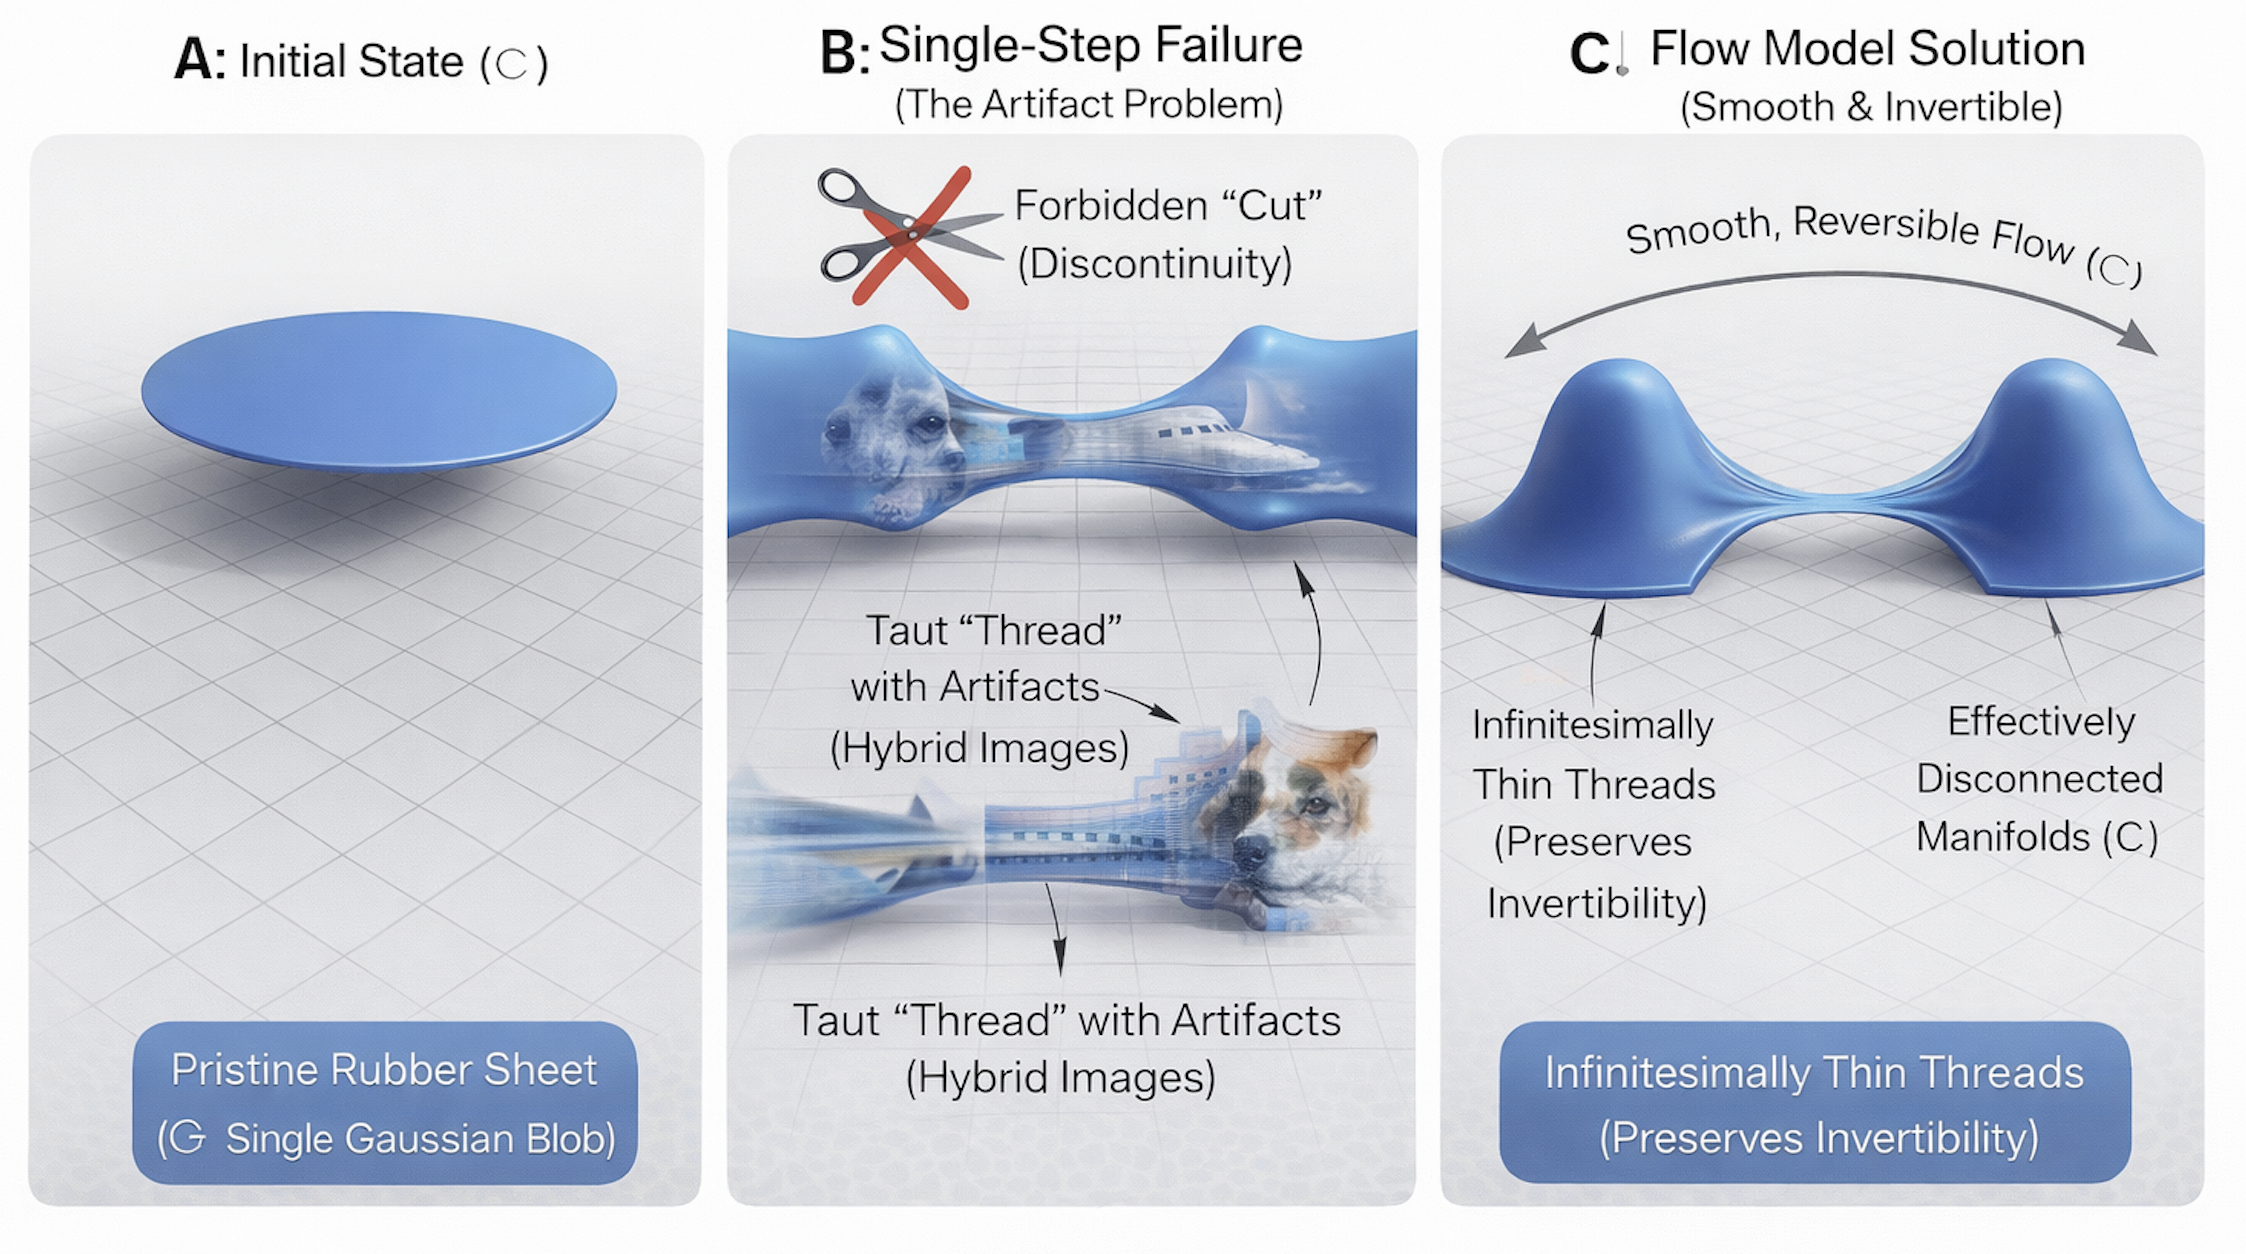
\includegraphics[width=0.7\textwidth]{images/rubber-sheet-analogy.png}
    \caption{ The Rubber Sheet Analogy. (A) Initial state. (B) A single-step model cannot 'cut' to form islands, creating artifact-filled rubber bands. (C) A flow model smoothly stretches the sheet over time into effectively disconnected manifolds connected by infinitesimally thin, invertible rubber bands.}
    \label{fig:topology_rubber_sheet}
\end{figure}

\subsection{Probability Density vs. Probability Mass}
Before proceeding further, we must understand the distinction between probability density and probability mass. In continuous spaces like $\mathbb{R}^d$, the probability of sampling exactly a specific data point $x$ is counter-intuitively exactly \textit{zero}. Wait, what? Yes, this is true, and the reason is very simple. In continuous space $\mathbb{R}^d$, there are infinitely many data points, and if the probability mass assigned to each of the data points was some non-zero value, no matter how small, summing up their probability mass would give us infinity, whereas, we know that the probability mass of a given space must always sum up to $1$. To get around this challenge, we use two distinct concepts:

\begin{itemize}
    \item \textbf{Probability Density $p(x)$:} Represents density—probability per unit volume. It tells us how concentrated probability is near $x$.
    \item \textbf{Probability Mass:} To get actual probability, we must multiply density by volume. For a small region $R$ around $x$, $P(R) \approx p(x) \cdot \text{Volume}(R)$. So,  while probability mass assigned to $x$ is always zero, probability mass within a volume $R$ around $x$ maybe non-zero.
\end{itemize}

In high dimensions, volumes are counterintuitively small. A hypercube with side length $0.1$ in 3 million dimensions has a volume of effectively zero ($0.1^{3,000,000}$). If probability mass flows into the small region $R$ around $x$, the probability density $p(x)$ rises, increasing the probability of sampling a data point around $x$. Conversely, if mass flows out, $p(x)$ falls. 

\subsection{Defining the Fields}
Flow models are concerned with the flow of probability mass. To understand the math underlying this flow, we need to define two fundamental mathematical formulations:

\textbf{1. The Probability Density Field $p_t(x)$:}
A scalar field $p_t: \mathbb{R}^d \times [0, 1] \to \mathbb{R}_{\geq 0}$. The scalar $p_t(x)$ represents how concentrated probability mass is near location $x \in \mathbb{R}^d$ at time $t \in [0,1]$. 

\textbf{2. The Velocity Vector Field $u_t(x)$:}
A vector field $u_t: \mathbb{R}^d \times [0, 1] \to \mathbb{R}^d$. The vector $u_t(x)$ points in the direction probability mass would move if it were located at position $x \in \mathbb{R}^d$ at time $t \in [0,1]$.

\begin{figure}[t]
    \centering
    \includegraphics[width=\textwidth]{images/eulerian_lagrangian_probability_flow.png}
    \caption{Eulerian vs.\ Lagrangian views of probability mass flow.
    }
    \label{fig:eulerian-lagrangian-probability}
\end{figure}

\subsection{Eulerian vs. Lagrangian View}
Having defined the density and velocity fields, we now establish the mathematical framework for tracking how probability mass moves through  $\mathbb{R}^d$ space. In fluid dynamics, there are two distinct ways to observe this motion, distinguished by how they treat the control volume containing the mass:

\begin{itemize}
    \item \textbf{The Eulerian View (The Fixed Volume):}
    In this perspective, we stand still and observe a specific, fixed point $x$ in $\mathbb{R}^d$ space. Imagine a tiny, fixed hyperspherical volume centered at $x$. We watch probability mass flow \textit{through} this fixed volume.
    If the velocity field $u_t(x)$ directs more mass into the hypersphere than flows out, the density $p_t(x)$ inside the hypersphere increases. If more flows out, the density decreases. This view focuses on the rate of change of probability density at a fixed point $x$ in $\mathbb{R}^d$ space.

    \item \textbf{The Lagrangian View (The Moving Volume):}
    In this perspective, we attach ourselves to a specific hyperspherical "blob" of probability mass and ride along with it as it flows through the $\mathbb{R}^d$ space. Imagine the blob is located at some point $x_0$ at time $t=0$. As time $t$ evolves from $t=0$ toward $t=1$, we do not stay at the point $x_0$; we move with the flow, guided by the vector field $u_t(x)$.

    
    Crucially, the blob we are attached to does not remain a hypersphere. As it moves through the complex velocity field $u_t(x)$, the blob deforms—stretching and compressing into new shapes—as it bumps into other moving blobs of probability mass. The total amount of probability mass inside the blob remains constant throughout the journey. However, the probability density $p_t(x)$ at a point $x$ inside the blob at time $t$ rises as the blob volume compresses, and falls as the blob volume expands.
\end{itemize}

For reasons that will become clear later, for training flow models, we prefer the Eulerian perspective, and for inference, we prefer the Lagrangian perspective. However, it is important to keep in mind that the two perspectives are describing the same phenomena.

\section{The Eulerian Perspective}

\subsection{The Cosmic Nebula}

To intuitively understand the Eulerian perspective and prepare for the upcoming mathematical formulations, consider the following analogy. Imagine our vector space $\mathbb{R}^d$ is a vast, static region of outer space (Figure \ref{fig:cosmic_nebula}).


\begin{figure}[h]
    \centering
    \includegraphics[width=0.7\textwidth]{images/cosmic-nebula.png}
   \caption{The Cosmic Nebula Analogy for Flow Matching. (1) The initial state is a uniform, shapeless mist of probability mass ($p_{init}$). (2) The target state is a structured "galaxy" of dense data points ($p_{data}$), such as stars. (3) Instead of learning the complex global dynamics directly, we model the flow as the superposition of simple "gravitational pulls" toward individual stars (conditional vector fields). (4) The complex global vector field $u_t(x)$ naturally emerges from the sum of these simple conditional fields, successfully transporting the shapeless mist into the target galaxy structure.}
    \label{fig:cosmic_nebula}
\end{figure}


\textbf{1. The Fluid (The Gas Cloud):}
Initially, this region is filled with a thin, uniform mist of hydrogen gas ($p_{init}$). This represents our probability mass. It is shapeless and spread everywhere.

\textbf{2. The Goal (The Galaxy):}
We want this shapeless mist to collapse and concentrate into specific, dense pockets—stars and planets—that form a galaxy ($p_{data}$). Each star or planet in the galaxy  represents a valid data sample $z$ in our data distribution, similar to an image in a data distribution of images.

\textbf{3. The Mechanism (The Gravity Field):}
We cannot touch the gas directly to move it. We can only manipulate the gravitational forces in the region. At every point $x$ in space, we define a "pull" vector ($u_t$). The gas simply obeys this field and moves according to it.

\textbf{Flux Superposition (The Key Insight):}
How do we determine the complex gravitational field needed to form a whole galaxy from the uniform mist? Imagine that every future star or planet ($z$) exerts its own simple, independent pull.
\begin{itemize}
    \item Star A pulls gas toward itself.
    \item Star B pulls gas toward itself.
\end{itemize}
At any point $x$ in the empty space, the total "flow" of gas is simply the weighted sum of the flows caused by Star A and Star B. If we want to train a "Gravitational Field" (our Neural Network), we don't need to teach it the complex global gravitational field of the galaxy. We simply teach it: "If you are here, and you want to form Star A, pull this way." By learning these simple, conditional pulls, the network implicitly learns the complex global field needed to sculpt the nebula. This insight—that the complex global field is just the superposition of simple conditional fields—is the key concept underlying all the math in this chapter. Now, let us boldly go into the mathematical formulations needed to understand flow models, starting with the Continuity Equation.

\subsection{The Continuity Equation}

\begin{figure}[t]
\centering
\includegraphics[width=0.7\textwidth]{images/continuity-equation.png}
\caption{Visualizing the Continuity Equation. The equation links the change in density at a fixed point to the geometry of the flow. Left: When flux converges (negative divergence), mass accumulates, and density rises. Right: When flux diverges (positive divergence), mass vacates the region, and density falls. This mechanism conserves total probability mass.}
\label{fig:continuity_eq_viz}
\end{figure}

The flow of probability mass at a point $x$ at time $t$ is governed by the Continuity Equation (Figure \ref{fig:continuity_eq_viz}), which ensures conservation of probability mass:

\begin{equation} \label{eq:continuity}
\frac{\partial p_t(x)}{\partial t} + \nabla \cdot (p_t(x) u_t(x)) = 0
\end{equation}


Let us unpack the terms:
\begin{itemize}
    \item $\frac{\partial p_t(x)}{\partial t}$: The rate of change of probability density at a fixed point $x$.
    \item $p_t(x) u_t(x)$: The \textbf{flux}, representing the rate of probability mass flow. To understand why this product represents flow, consider the physical dimensions:
\[
\underbrace{p_t(x)}_{\frac{\text{Mass}}{\text{Volume}}} \times \underbrace{u_t(x)}_{\frac{\text{Distance}}{\text{Time}}} = \underbrace{\text{Flux}}_{\frac{\text{Mass}}{\text{Area} \cdot \text{Time}}}
\]
Intuitively, density tells us \textit{how crowded} the probability mass is, and velocity tells us \textit{how fast} it is moving. Multiplying them yields the amount of probability mass passing through a unit surface at $x$ per unit of time.
    \item $\nabla \cdot (\dots)$: The \textbf{divergence} operator, measuring the net outflow of flux from a region.
\end{itemize}

The Continuity Equation (Figure \ref{fig:continuity_eq_viz}) states: \textit{The rate at which probability density increases at a point equals the negative of the net outflow of flux.} Mathematically, divergence is the sum of partial derivatives:
\begin{equation}
\nabla \cdot F(x) = \sum_{i=1}^d \frac{\partial F_i}{\partial x_i}
\end{equation}

If divergence is positive, probability mass is spreading out (leaving the region), causing probability density to drop. If divergence is negative, probability mass is converging (entering the region), causing the probability density to rise. This mechanism allows the velocity field to "sculpt" the probability density, transporting probability mass from the initial noise distribution to the target data distribution without ever creating or destroying probability.


\section{Flow Matching: Learning to Transport Probability}

With the continuity equation established, we now address the central question of flow-based generative modeling: how do we learn a velocity field that transports the initial distribution $p_{\text{init}}$ to the data distribution $p_{\text{data}}$? Flow matching provides an elegant answer.

The key insight of flow matching is that we do not need to learn the complete, global velocity field (the complex gravitational field of the whole galaxy) directly. Instead, we decompose the problem into learning many simple, conditional velocity fields (the independent pull of a single star) and show that their superposition automatically yields the correct marginal (global) velocity field.

\subsection{Probability Density Decomposition}

We begin with the observation that the probability density distribution $p_t(x)$ can be written as an integral over conditional probability density distributions. To visualize this, we introduce the concept of \textbf{Probability Cones}.
Let $z$ denote a specific sample (a target star, or an image) from the data distribution, so $z \sim p_{\text{data}}(z)$.
Consider the conditional distribution $p_t(x|z)$. At $t=0$, this distribution is wide and diffuse (the uniform mist, or meaningless images with static). As $t \to 1$, this distribution must concentrate entirely onto the specific target $z$ (a star, or a valid image). Geometrically, we can visualize $p_t(x|z)$ as a \textit{cone of probability mass} in spacetime:
\begin{itemize}
    \item \textbf{The Base ($t=0$):} The cone is wide, representing the uncertainty of the initial noise state.
    \item \textbf{The Tip ($t=1$):} The cone narrows to a sharp point exactly at $z$.
\end{itemize}

The marginal density $p_t(x)$ is simply the superposition (mixture) of all these overlapping cones. Mathematically:

\begin{equation} \label{eq:marginal_density}
p_t(x) = \int p_t(x|z) \, p_{\text{data}}(z) \, dz
\end{equation}

This decomposition is a standard marginalization: to get the total probability density at any point $x$ and time $t$, we sum the contributions from every "probability cone" passing through that point. If $x$ is located where many cones overlap, the marginal density $p_t(x)$ will be high. If $x$ is in a region traversed by few cones, the density will be low.

\begin{figure}[h]
    \centering
        \includegraphics[width=0.7\textwidth]{images/prob-cone.png}
    \caption{Visualizing Marginal Probability Density Decomposition. Each target data point $z$ defines a "cone" of conditional probability $p_t(x|z)$ that focuses mass from the noise distribution ($t=0$) to the target ($t=1$). The global marginal density $p_t(x)$ is the sum of these overlapping cones.}
    \label{fig:probability_cones}
\end{figure}

\subsection{Deriving the Vector Field}

The power of this decomposition becomes apparent when we consider velocity fields. For each conditional path $p_t(x|z)$, we assume there exists a corresponding conditional velocity field $u_t(x|z)$ that satisfies the continuity equation locally:

\begin{equation} \label{eq:conditional_continuity}
\frac{\partial p_t(x|z)}{\partial t} + \nabla \cdot (p_t(x|z) u_t(x|z)) = 0
\end{equation}

This equation states that for each fixed target $z$, the probability mass flowing toward $z$ evolves according to its own velocity field $u_t(x|z)$. The crucial question is: what velocity field governs the evolution of the marginal density $p_t(x)$?

To answer this, we take the time derivative of the marginal density equation (\ref{eq:marginal_density}). Since $p_{\text{data}}(z)$ does not depend on time, we can bring the derivative inside the integral using the Leibniz integral rule:

\begin{equation}
\frac{\partial p_t(x)}{\partial t} = \frac{\partial}{\partial t} \int p_t(x|z) \, p_{\text{data}}(z) \, dz = \int \frac{\partial p_t(x|z)}{\partial t} \, p_{\text{data}}(z) \, dz
\end{equation}

Now we substitute the conditional continuity equation (\ref{eq:conditional_continuity}) for $\frac{\partial p_t(x|z)}{\partial t}$:

\begin{equation}
\frac{\partial p_t(x)}{\partial t} = \int \left( -\nabla \cdot (p_t(x|z) u_t(x|z)) \right) p_{\text{data}}(z) \, dz
\end{equation}

The divergence operator is linear, meaning $\nabla \cdot (aF + bG) = a(\nabla \cdot F) + b(\nabla \cdot G)$. This allows us to bring the divergence outside the integral:

\begin{equation}
\frac{\partial p_t(x)}{\partial t} = -\nabla \cdot \left( \int p_t(x|z) u_t(x|z) p_{\text{data}}(z) \, dz \right)
\end{equation}

Comparing this result with the marginal continuity equation \ref{eq:continuity}, we identify that the marginal flux must equal the integrated conditional flux. Dividing both sides by $p_t(x)$ yields the fundamental result of flow matching:

\begin{equation} \label{eq:marginal_velocity}
u_t(x) = \frac{1}{p_t(x)} \int u_t(x|z) \, p_t(x|z) \, p_{\text{data}}(z) \, dz
\end{equation}

Using Bayes' rule, we can rewrite this as a posterior expectation. The probability that a sample at $x$ belongs to a trajectory targeting $z$ is:

\begin{equation}
p_{\text{data}}(z|x, t) = \frac{p_t(x|z) p_{\text{data}}(z)}{p_t(x)}
\end{equation}

Thus:

\begin{equation}
u_t(x) = \mathbb{E}_{z \sim p_{\text{data}}(\cdot|x,t)} [u_t(x|z)]
\end{equation}

This interpretation connects to our nebula analogy: the global velocity at a point is the average of the specific pulls from all possible stars, weighted by the likelihood that the mass at that point is destined for each star.

\subsection{The Flow Matching Objective}

Equation (\ref{eq:marginal_velocity}) defines the target field $u_t(x)$, but computing it requires an intractable integral over the entire dataset. To train a neural network $v_\theta(x, t)$ to approximate this field, we ideally want to minimize the global error:

\begin{equation} \label{eq:loss_fm_ideal}
\mathcal{L}_{\text{FM}}(\theta) = \mathbb{E}_{t \sim \mathcal{U}(0,1)} \mathbb{E}_{x \sim p_t(x)} \left[ \| v_\theta(x, t) - u_t(x) \|^2 \right]
\end{equation}

Since $u_t(x)$ is intractable, we define a simpler objective called \textbf{Conditional Flow Matching} (CFM). Instead of matching the aggregated marginal field, we match the simple conditional fields individually:

\begin{equation} \label{eq:loss_cfm}
\mathcal{L}_{\text{CFM}}(\theta) = \mathbb{E}_{t \sim \mathcal{U}(0,1)} \mathbb{E}_{z \sim p_{\text{data}}} \mathbb{E}_{x \sim p_t(x|z)} \left[ \| v_\theta(x, t) - u_t(x|z) \|^2 \right]
\end{equation}

Crucially, all terms in $\mathcal{L}_{\text{CFM}}$ are tractable and easy to sample. We now prove that these two objectives are equivalent for optimization.

\subsection{Theorem: Objective Equivalence}

We now prove that minimizing the tractable conditional loss $\mathcal{L}_{\text{CFM}}$ is equivalent to minimizing the intractable marginal loss $\mathcal{L}_{\text{FM}}$.

\begin{theorem}[Flow Matching Objective Equivalence]
The gradients of the marginal flow matching objective $\mathcal{L}_{\text{FM}}(\theta)$ and the conditional flow matching objective $\mathcal{L}_{\text{CFM}}(\theta)$ with respect to the parameters $\theta$ are equal:
\begin{equation}
\nabla_\theta \mathcal{L}_{\text{FM}}(\theta) = \nabla_\theta \mathcal{L}_{\text{CFM}}(\theta)
\end{equation}
\end{theorem}

\begin{proof}
We begin by writing the marginal objective $\mathcal{L}_{\text{FM}}$ in its explicit integral form, expanding the expectation over time and space:
\begin{equation}
\mathcal{L}_{\text{FM}}(\theta) = \int_0^1 \int_{\mathbb{R}^d} p_t(x) \| v_\theta(x, t) - u_t(x) \|^2 \, dx \, dt
\end{equation}

\textbf{Step 1: Expand the Marginal Loss} \\
We expand the squared norm $\|a - b\|^2 = \|a\|^2 - 2\langle a, b \rangle + \|b\|^2$, where $\langle a, b \rangle$ is the familiar dot product between $a$ and $b$:
\begin{equation}
\mathcal{L}_{\text{FM}}(\theta) = \int_0^1 \int_{\mathbb{R}^d} p_t(x) \left( \| v_\theta(x, t) \|^2 - 2 \langle v_\theta(x, t), u_t(x) \rangle + \| u_t(x) \|^2 \right) \, dx \, dt
\end{equation}
Since we are computing the gradient with respect to $\theta$, the term $\| u_t(x) \|^2$ is constant and vanishes. Thus:
\begin{equation} \label{eq:grad_fm_start}
\nabla_\theta \mathcal{L}_{\text{FM}}(\theta) = \nabla_\theta \int_0^1 \underbrace{\int_{\mathbb{R}^d} p_t(x) \| v_\theta(x, t) \|^2 \, dx}_{\text{Term 1}} - \nabla_\theta \int_0^1 \underbrace{2 \int_{\mathbb{R}^d} p_t(x) \langle v_\theta(x, t), u_t(x) \rangle \, dx}_{\text{Term 2}} \, dt
\end{equation}

\textbf{Step 2: Analyze the Cross-Term (Term 2)} \\
We substitute the definition of the marginal vector field $u_t(x)$ from Eq. (\ref{eq:marginal_velocity}) into the inner integral of Term 2:
\begin{equation}
u_t(x) = \frac{1}{p_t(x)} \int p_t(x|z) p_{\text{data}}(z) u_t(x|z) \, dz
\end{equation}
The integral becomes:
\begin{align}
\int_{\mathbb{R}^d} p_t(x) \langle v_\theta(x, t), u_t(x) \rangle \, dx &= \int_{\mathbb{R}^d} p_t(x) \left\langle v_\theta(x, t), \frac{1}{p_t(x)} \int p_t(x|z) p_{\text{data}}(z) u_t(x|z) \, dz \right\rangle dx
\end{align}
The $p_t(x)$ terms cancel out. By the linearity of the inner product and Fubini's theorem (swapping the order of integration), we get:
\begin{align}
&= \int_{\mathbb{R}^d} \int \langle v_\theta(x, t), u_t(x|z) \rangle p_t(x|z) p_{\text{data}}(z) \, dz \, dx \\
&= \int \int_{\mathbb{R}^d} p_t(x|z) p_{\text{data}}(z) \langle v_\theta(x, t), u_t(x|z) \rangle \, dx \, dz \label{eq:fm_term2_final}
\end{align}

\textbf{Step 3: Analyze the Squared Term (Term 1)} \\
We use the marginalization identity $p_t(x) = \int p_t(x|z) p_{\text{data}}(z) \, dz$ to rewrite the first term:
\begin{align}
\int_{\mathbb{R}^d} p_t(x) \| v_\theta(x, t) \|^2 \, dx &= \int_{\mathbb{R}^d} \left( \int p_t(x|z) p_{\text{data}}(z) \, dz \right) \| v_\theta(x, t) \|^2 \, dx \\
&= \int \int_{\mathbb{R}^d} p_t(x|z) p_{\text{data}}(z) \| v_\theta(x, t) \|^2 \, dx \, dz \label{eq:fm_term1_final}
\end{align}

\textbf{Step 4: Compare with Conditional Loss} \\
Now, let us write the explicit integral form of the Conditional Flow Matching loss $\mathcal{L}_{\text{CFM}}$:
\begin{align}
\mathcal{L}_{\text{CFM}}(\theta) &= \int_0^1 \int \int_{\mathbb{R}^d} p_t(x|z) p_{\text{data}}(z) \| v_\theta(x, t) - u_t(x|z) \|^2 \, dx \, dz \, dt \\
&= \int_0^1 \int \int_{\mathbb{R}^d} p_t(x|z) p_{\text{data}}(z) \left( \| v_\theta \|^2 - 2 \langle v_\theta, u_t(x|z) \rangle + \| u_t(x|z) \|^2 \right) dx \, dz \, dt
\end{align}
Comparing Eq. (\ref{eq:fm_term1_final}) and Eq. (\ref{eq:fm_term2_final}) with this expansion, we see that the terms dependent on $\theta$ are identical. Specifically:
\begin{itemize}
    \item The $\| v_\theta \|^2$ term in $\mathcal{L}_{\text{CFM}}$ integrates to exactly Term 1 of $\mathcal{L}_{\text{FM}}$.
    \item The cross-term in $\mathcal{L}_{\text{CFM}}$ integrates to exactly Term 2 of $\mathcal{L}_{\text{FM}}$.
\end{itemize}
Since the remaining term $\| u_t(x|z) \|^2$ does not depend on $\theta$, the gradients are identical.
\end{proof}

\subsection{The Training Algorithm}

The equivalence theorem allows us to implement a highly efficient training loop. We simply sample random data points, random times, and random points along the conditional paths, then optimize the network to match the conditional velocity. The beauty of this algorithm is its simplicity. Each step involves a trivial regression task: "given that I am here and want to go there, what is my velocity?" Yet, the aggregate result of this training is a network that solves the complex, global transport problem defined by the nebula analogy.

\begin{algorithm}
\caption{Conditional Flow Matching Training Loop}
\label{alg:cfm_training}
\begin{algorithmic}[1]
\Require Training dataset $\mathcal{D}$ (samples from $p_{\text{data}}$)
\Require Neural network $v_\theta(x, t)$
\Require Conditional path sampler returning $x \sim p_t(x|z)$ and target $u_t(x|z)$
\Require Learning rate $\eta$

\While{not converged}
    \State Sample batch of data points $z \sim \mathcal{D}$
    \State Sample batch of times $t \sim \mathcal{U}(0, 1)$
    \State Sample $x_0 \sim p_{\text{init}}$

    \State \textbf{Compute Location and Target:}
    \State $x \leftarrow \text{SampleLocation}(z, t, x_0)$ \Comment{e.g., $(1-t)x_0 + tz$}
    \State $u \leftarrow \text{ComputeConditionalVelocity}(z, t, x)$ \Comment{e.g., $z - x_0$}

    \State \textbf{Forward Pass:}
    \State $\hat{v} \leftarrow v_\theta(x, t)$

    \State \textbf{Optimization:}
    \State $\mathcal{L} \leftarrow \| \hat{v} - u \|^2$ \Comment{Mean Squared Error}
    \State $\theta \leftarrow \theta - \eta \nabla_\theta \mathcal{L}$ \Comment{Gradient Descent Update}
\EndWhile
\end{algorithmic}
\end{algorithm}


\subsection{Conditional Flow Matching}

In the Flow Matching framework, we define a time-dependent probability path $p_t$ that continuously transforms a source distribution $p_0$ (e.g., standard Gaussian noise) to a target distribution $p_1$ (e.g., data).

We construct this path using a simple linear interpolation (displacement map). For a source sample $x_0 \sim p_0$ and a target data point $x_1 \sim p_1$, we define the intermediate state $x_t$ at time $t \in [0, 1]$ as:

\begin{equation} \label{eq:fm_path}
x_t = \psi_t(x_0, x_1) = (1 - t) x_0 + t x_1
\end{equation}

This parameterization ensures that at $t=0$, we have $x_0$ (noise), and at $t=1$, we reach $x_1$ (data). The trajectory is a straight line connecting the source and target.

\subsubsection*{Deriving the Target Vector Field}
The objective of Flow Matching is to learn a velocity field $u_t(x)$ that generates this path. The target velocity $u_t$ for a specific pair $(x_0, x_1)$ is simply the time derivative of the trajectory defined in Equation (\ref{eq:fm_path}).

Differentiating $x_t$ with respect to time $t$:

\begin{equation} \label{eq:time_derivative}
\frac{dx_t}{dt} = \frac{d}{dt} \left[ (1 - t) x_0 + t x_1 \right]
\end{equation}

Since $x_0$ and $x_1$ are constant with respect to time for a given trajectory, the derivative simplifies to:

\begin{equation}
\frac{dx_t}{dt} = -x_0 + x_1
\end{equation}

Thus, the conditional vector field is constant in time:

\begin{equation} \label{eq:fm_velocity}
u_t(x|x_0, x_1) = x_1 - x_0
\end{equation}

\subsubsection*{Training Objective}
The neural network $v_\theta(t, x)$ approximates this vector field. Since the model does not know which specific $x_0$ and $x_1$ generated the current point $x$, it learns the expected velocity conditioned on the current location. This is achieved by minimizing the Conditional Flow Matching loss:

\begin{equation}
\mathcal{L}_{CFM}(\theta) = \mathbb{E}_{t \sim [0,1], x_0 \sim p_0, x_1 \sim p_1} \left[ \| v_\theta(t, x_t) - (x_1 - x_0) \|^2 \right]
\end{equation}

where $x_t$ is sampled according to Equation (\ref{eq:fm_path}).

\subsection{From Independent Couplings to Optimal Transport}

While the linear conditional path defined above ($x_t = (1-t)x_0 + t x_1$) provides a mathematically simple objective for Flow Matching, its efficiency depends heavily on how the source samples $x_0$ and target samples $x_1$ are paired.

\subsubsection*{Advantages of the Linear Path}
The primary advantage of this formulation is its simplicity and stability.
\begin{itemize}
    \item \textbf{Analytic Vector Fields:} The target velocity $u_t = x_1 - x_0$ is constant for each trajectory, requiring no complex ODE or SDE solvers during training.
    \item \textbf{Straight Trajectories:} Straight paths are the shortest distance between two points, theoretically minimizing the integration error during sampling compared to curved diffusion paths.
\end{itemize}

\subsubsection*{The Problem of Arbitrary Couplings}
However, the standard formulation assumes an \textit{independent coupling} between the source and target distributions. We sample $x_0 \sim p_0$ and $x_1 \sim p_1$ independently, meaning any noise sample can be paired with any data sample.

This randomness leads to significant inefficiencies:
\begin{itemize}
    \item \textbf{Crossing Paths:} Since the pairing is random, trajectories frequently cross each other. For example, a noise sample in the top-left quadrant might be mapped to a data point in the bottom-right, while a nearby noise sample maps to the top-left.
    \item \textbf{High-Variance Vector Fields:} The neural network $v_\theta(t, x)$ attempts to learn the marginal vector field. When paths cross at a point $x$, the network receives conflicting gradient signals (e.g., one path says "go right," another says "go left"). This forces the network to learn the average of these conflicts, resulting in a turbulent, harder-to-learn vector field.
    \item \textbf{Wasted Kinetic Energy:} The total distance traveled by the probability mass is far higher than necessary. The system expends "energy" moving mass across the entire domain rather than mapping it to the nearest valid data point.
\end{itemize}

\subsubsection*{Motivation for Optimal Transport}
To resolve these issues, we need to replace the random independent coupling with an \textit{optimal coupling}. Instead of sampling $x_0$ and $x_1$ independently, we seek a joint distribution $\pi(x_0, x_1)$ that minimizes the total transport cost:

\begin{equation}
\mathcal{C}(\pi) = \int \| x_1 - x_0 \|^2 d\pi(x_0, x_1)
\end{equation}

This is the Monge-Kantorovich Optimal Transport problem. By aligning $x_0$ and $x_1$ such that the total squared distance is minimized, we ensure that trajectories are straight and, crucially, do not cross.



\subsubsection*{Why Trajectories Do Not Cross: Cyclical Monotonicity}

The non-crossing property is not merely an aesthetic preference; it is a fundamental geometric consequence of cost minimization. Consider the simplest case of two source points $x_a, x_b$ and two target points $y_a, y_b$.

If we pair $(x_a \to y_b)$ and $(x_b \to y_a)$ such that their paths intersect, we can almost always reduce the total transport distance by swapping the targets to $(x_a \to y_a)$ and $(x_b \to y_b)$. This "uncrossing" operation reduces the global cost. Since Optimal Transport seeks the \textit{minimum} possible global cost, the resulting paths must be free of such crossings.

Mathematically, this is formalized as \textbf{Cyclical Monotonicity}. A transport map $T$ is cyclically monotonic if, for any sequence of points $(x_1, y_1), \dots, (x_k, y_k)$ in the transport plan, permuting the targets cannot lower the cost:

\begin{equation}
\sum_{i=1}^k \| x_i - y_i \|^2 \leq \sum_{i=1}^k \| x_i - y_{i+1} \|^2
\end{equation}

where $y_{k+1} = y_1$.

\subsection{Optimal Transport: The Monge-Kantorovich Problem}

Optimal transport addresses a fundamental question: given two probability distributions $\mu$ (the source) and $\nu$ (the target), what is the most efficient way to transform one into the other? Here, "efficient" is measured by a cost function $c(x, y)$ that quantifies the penalty or effort required to move a unit of probability mass from location $x$ to location $y$.

\subsubsection{The Monge Formulation (Deterministic Transport)}
The classical formulation, proposed by Gaspard Monge in 1781 \cite{monge1781memoire}, frames this as a deterministic mapping problem. We seek a transport map function $T: \mathbb{R}^d \to \mathbb{R}^d$ that moves every particle from the source probability distribution $\mu$ to a specific location in the target probability distribution $\nu$ such that the total transport cost is minimized.

The objective function is:
\begin{equation}
\min_{T} \int c(x, T(x)) \, d\mu(x) \quad \text{subject to} \quad T_\# \mu = \nu
\end{equation}

\textbf{Understanding the Objective}:
The integral represents the \textit{total global cost}. For every infinitesimal unit of probability mass located at $x$ in the source distribution, we pay a cost $c(x, T(x))$ to move it to its destination $T(x)$. By integrating over the entire source domain, we sum up the costs for moving all probability mass. The ``min'' operator seeks the specific function $T$ that yields the lowest possible sum.

\textbf{Understanding the Pushforward Constraint} ($T_\# \mu = \nu$):
The notation $T_\# \mu = \nu$ is the formal constraint ensuring that the map $T$ actually reconstructs the target distribution. It is defined by the requirement that for any measurable region (set) $A$ in the target space:
\begin{equation}
\nu(A) = \mu(T^{-1}(A))
\end{equation}
Let us unpack this definition:
\begin{itemize}
    \item \textbf{The Set $A$}: Imagine $A$ is a specific region in the target space (e.g., a set of images). The value $\nu(A)$ represents the total probability mass that must end up inside this set.
    \item \textbf{The Pre-image} $T^{-1}(A)$: This represents the set of all starting locations $x$ that the map $T$ sends into the set $A$.
    \item \textbf{Conservation of Mass}: The equation states that the total mass arriving in region $A$ ($\nu(A)$) must exactly equal the total mass that started in the source region $T^{-1}(A)$ ($\mu(T^{-1}(A))$).
\end{itemize}
In simple terms, the map $T$ must rearrange the mass such that the shape of the probability cloud changes from $\mu$ to $\nu$ without creating or destroying any probability mass.

\subsubsection{The Kantorovich Relaxation (Probabilistic Transport)}
The Monge formulation has a critical flaw: it forbids splitting probability mass. If the source is a single pile of probability mass (a Dirac delta probability distribution) and the target is two smaller piles, no function $T$ can map the single pile to two different target piles simultaneously.

Leonid Kantorovich solved this in 1942 \cite{kantorovich1942translocation} by relaxing the problem. Instead of a deterministic map $T(x)$, we solve for a \textbf{transport plan} (or coupling) $\pi(x, y)$. This is a joint probability distribution where $\pi(x, y)$ represents the amount of mass moved from $x$ to $y$.

The optimization problem becomes:
\begin{equation}
\min_{\pi \in \Pi(\mu, \nu)} \int c(x, y) \, d\pi(x, y)
\end{equation}

Here, $\Pi(\mu, \nu)$ is the set of all valid joint distributions where the marginals sum to $\mu$ and $\nu$ respectively.
\begin{itemize}
    \item \textbf{What is being minimized?} We integrate the cost $c(x, y)$ weighted by the amount of mass $\pi(x, y)$ moving between those points. We search for the plan $\pi$ that results in the lowest expected cost.
    \item \textbf{Why is this better?} A transport plan allows "mass splitting." One unit of mass at $x$ can be sent partially to $y_1$ and partially to $y_2$, enabling solutions where Monge's formulation fails.
\end{itemize}

\subsubsection{The Wasserstein Distance and the Earth Mover's Analogy}
When the cost function is the squared Euclidean distance $c(x, y) = \|x - y\|^2$, the minimum value of the objective function defines a metric known as the \textbf{Wasserstein-2 Distance} ($W_2$):

\begin{equation}
W_2(\mu, \nu) = \left( \inf_{\pi \in \Pi(\mu, \nu)} \int \|x - y\|^2 \, d\pi(x, y) \right)^{1/2}
\end{equation}



\textbf{Deconstructing the Equation}:
To understand this definition, let us break it down term by term:
\begin{itemize}
    \item \textbf{The Cost Integral} ($\int \|x - y\|^2 d\pi$): This term calculates the \textit{expected squared distance} mass travels under a specific transport plan $\pi$. It represents the total "effort" for that specific strategy.
    \item \textbf{The Infimum} ($\inf$): "inf" stands for \textbf{infimum}, which is the mathematical generalization of "minimum." It tells us to search through \textit{every possible valid transport plan} $\pi$ in the set $\Pi(\mu, \nu)$ and find the one that results in the lowest possible cost. We are not interested in just any plan; we want the \textit{optimal} one.
    \item \textbf{The Square Root} $(\dots)^{1/2}$: Finally, we take the square root of the minimum cost. This is analogous to taking the square root of variance to get standard deviation; it ensures the "units" of the Wasserstein distance match the units of the data space (e.g., pixel intensity) rather than the squared units.
\end{itemize}

\textbf{Distance Between Distributions}:
In standard geometry, we measure the distance between two points. The Wasserstein distance generalizes this concept to measure the ``distance'' between two probability distributions (entire shapes). If $\mu$ and $\nu$ are identical, the cost is zero (mass stays put). If they are disjoint, the distance is determined by how far the mass must travel to transform one into the other.

\textbf{The Earth Mover's Analogy}:
This metric is frequently called the Earth Mover's Distance because of a vivid physical intuition:
\begin{itemize}
    \item \textbf{The Setup}: Imagine the source distribution $\mu$ is a pile of earth (dirt) of a certain shape, and the target distribution $\nu$ is a hole (trench) of a different shape but equal volume.
    \item \textbf{The Task}: You must shovel the earth into the hole.
    \item \textbf{The Cost}: The effort required to move a shovel-load of earth is proportional to the squared distance it is moved.
    \item \textbf{The Metric}: The Earth Mover's Distance is the \textit{minimum possible total work} required to completely fill the hole with the pile.
\end{itemize}

Unlike other metrics (like \textbf{KL-divergence}) which look at pointwise overlap, the \textbf{Wasserstein distance} respects the underlying geometry of the space. Even if two distributions have zero overlap, if they are close to each other in space, the Earth Mover's Distance will be small, whereas \textbf{KL-divergence} would be infinite. This geometric awareness is why Optimal Transport is so powerful for generative modeling.

Our interest in optimal transport stems from its connection to probability flows. Rather than viewing transport as an instantaneous relocation, we can frame it as a dynamical problem: find a time-dependent velocity field that moves probability mass from $\mu$ to $\nu$ while minimizing kinetic energy. This is the Benamou-Brenier formulation \cite{benamou2000computational}, which we now develop in detail.

\subsection{The Benamou-Brenier Formulation}

The Benamou-Brenier formulation \cite{benamou2000computational} recasts Optimal Transport from a static coupling problem into a dynamic fluid mechanics problem. Instead of simply asking "which point maps to which?", we ask: "how does the probability mass move over time to minimize cost?" We seek a time-dependent probability density $p_t(x)$ and a velocity field $u_t(x)$ for $t \in [0, 1]$ that satisfy the following conditions:
\begin{itemize}
    \item \textbf{Boundary Conditions:} $p_0 = p_{\text{init}}$ (Source) and $p_1 = p_{\text{data}}$ (Target).
    \item \textbf{Mass Conservation:} The density evolves according to the continuity equation:
    \begin{equation}
    \frac{\partial p_t(x)}{\partial t} + \nabla \cdot (p_t(x) u_t(x)) = 0
    \end{equation}
    \item \textbf{Cost Minimization:} The total kinetic energy of the flow is minimized.
\end{itemize}

The kinetic energy functional $\mathcal{E}$ measures the total "cost" of the transport:
\begin{equation}
\mathcal{E}[p, u] = \int_0^1 \int_{\mathbb{R}^d} \frac{1}{2} p_t(x) \|u_t(x)\|^2 \, dx \, dt
\end{equation}
Physically, the term $\frac{1}{2} p_t(x) \|u_t(x)\|^2$ represents the kinetic energy density at a specific point $x$ and time $t$. We integrate this over all space and all time.

\subsubsection{Deriving the Optimal Velocity Field}
To determine the properties of the optimal velocity field, we employ the \textbf{Calculus of Variations}, a field of mathematical analysis that deals with maximizing or minimizing functionals (integrals).

\paragraph{Primer: The Method of Lagrange Multipliers}
To understand how we derive the optimal velocity field using the Calculus of Variations, we must first master the intuition behind the Method of Lagrange Multipliers.

Suppose we want to find the minimum value of a cost function $f(x)$ (e.g., minimizing energy) subject to a hard constraint $g(x) = c$ (e.g., staying on a specific path). We cannot simply find where the derivative of $f(x)$ is zero (the unconstrained minimum), because that optimal point might lie somewhere forbidden, outside the region defined by our constraint.

To solve this, we must think geometrically.

\begin{figure}[h]
    \centering
     \includegraphics[width=0.7\textwidth]{images/level_curves_gradient.png}
    \caption{Visualizing a scalar cost function $f$ using level curves. Each curve connects points of equal value. The gradient vectors $\nabla f$ (arrows) always point in the direction of steepest ascent and are everywhere perpendicular to the level curves.}
    \label{fig:level_curves_gradients}
\end{figure}

\textbf{Step 1: The Landscape (Level Curves)}
Imagine $f(x)$ represents the altitude of a terrain. We can visualize this terrain using \textbf{level curves} (or contour lines). A level curve is a line connecting all points with the same height. If you walk along a level curve, your elevation does not change.


\textbf{Step 2: The Path (The Constraint)}
The constraint equation $g(x) = c$ defines a specific path through this terrain. We are forced to walk only along this path. Our goal is to find the lowest point (point $x$ where $f(x)$ value is minimum) or the highest point (point $x$ where $f(x)$ value is maximum) that lies on this specific path.

\textbf{Step 3: The "Kissing" Condition}
Imagine walking along the path $g(x)=c$.
\begin{itemize}
    \item If the path crosses a level curve of $f$, you are moving from a higher elevation to a lower one (or vice versa). This means you have not reached the minimum yet; you can keep walking in that direction to lower your cost.
    \item You stop lowering your cost only when the path stops crossing level curves and instead runs \textit{along} one.
\end{itemize}
This occurs exactly where the constraint curve $g(x)=c$ just touches—or \textbf{"kisses"}—a level curve of $f(x)$. At this precise point of tangency, the path and the level curve share a \textbf{common tangent line}.


\textbf{Step 4: From Tangents to Gradients}
How do we express "common tangents" mathematically? We use gradients.
Recall a fundamental property of the gradient vector $\nabla f$: \textit{The gradient is always perpendicular (normal) to the level curve.}
\begin{itemize}
    \item If the level curve of $f$ and the constraint curve $g$ are tangent (share a line), then their perpendicular vectors (normals) must be parallel.
    \item Therefore, at the optimal point, the gradient of the cost $\nabla f$ must be parallel to the gradient of the constraint $\nabla g$.
\end{itemize}

We can express "parallel vectors" by stating that one is a scalar multiple of the other:
\begin{equation}
\nabla f(x) = \lambda \cdot \nabla g(x)
\end{equation}
The scalar $\lambda$ is the \textbf{Lagrange Multiplier}. It represents the ratio of the "forces" between the cost and the constraint.

\textbf{Step 5: The Lagrangian}
We can bundle this entire geometric argument into a single equation. We define the \textbf{Lagrangian} $\mathcal{L}$:
\begin{equation}
\mathcal{L}(x, \lambda) = f(x) - \lambda \cdot (g(x) - c)
\end{equation}
If we take the derivative of $\mathcal{L}$ with respect to $x$ and set it to zero, we get $\nabla f - \lambda \nabla g = 0$, which recovers our parallel gradient condition. If we differentiate with respect to $\lambda$, we recover the constraint $g(x) = c$. Thus, minimizing $\mathcal{L}$ solves the constrained problem.

\begin{figure}[t]
    \centering
    \includegraphics[width=0.85\linewidth]{images/lagrange_multipliers.png}
    \caption{
    Geometric interpretation of the Method of Lagrange Multipliers.
    Shown are level curves of the objective function $f(x)$, labeled
    $f = c_1, c_2, c_3$, with decreasing values toward the center, together
    with a constraint curve $g(x) = c$.
    The constrained optimum $x^\ast$ occurs at the point where the constraint
    curve is tangent to a level curve of $f$.
    At this point, the gradients $\nabla f(x^\ast)$ and $\nabla g(x^\ast)$ are
    parallel, illustrating the necessary optimality condition
    $\nabla f(x^\ast) = \lambda \nabla g(x^\ast)$.
    }
    \label{fig:lagrange-multipliers-geometry}
\end{figure}
\paragraph{Extension to Fields (Calculus of Variations)}
In our optimal transport problem, we apply this same logic, but we scale it up from finding a single point $x$ to finding entire functions.

\textbf{1. From Points to Fields}
In standard calculus, our variable $x$ is a vector in $\mathbb{R}^d$. In Optimal Transport, our "variables" are the density field $p_t(x)$ and velocity field $u_t(x)$ defined over all space and time. We are optimizing the "shape" of these functions.

\textbf{2. From One Constraint to Infinite Constraints}
In the simple primer, we had one constraint equation $g(x) = c$. In our flow problem, the constraint is the \textbf{Continuity Equation}:
\begin{equation}
\frac{\partial p_t(x)}{\partial t} + \nabla \cdot (p_t(x) u_t(x)) = 0
\end{equation}
Crucially, this equation must hold \textit{at every single point} in space $x$ and every moment in time $t$. This is effectively an infinite number of constraints—one for every coordinate $(x, t)$ in the $\mathbb{R}^d \times [0,1]$ space-time.

\textbf{3. The Multiplier becomes a Field}
Since we have a distinct constraint for every point in space-time, we need a distinct Lagrange multiplier for every point in space-time.
\begin{itemize}
    \item Just as a single constraint $g(x)=0$ gets a single scalar $\lambda$...
    \item ...a constraint defined everywhere $g(x,t)=0$ gets a \textbf{multiplier function} $\phi_t(x)$.
\end{itemize}

We call this function $\phi_t(x)$ the \textbf{potential field}. Intuitively, you can think of $\phi_t(x)$ as a "variable pressure" field. Just as physical pressure arises in a fluid to enforce the constraint that water cannot be compressed, the potential $\phi_t(x)$ arises in our optimization to enforce the constraint that probability mass is conserved. It pushes and pulls on the velocity field $u_t(x)$ locally to ensure the continuity equation is never violated.

\textbf{Step 1: Construct the Lagrangian} \\
We define the Lagrangian functional $\mathcal{L}$ by adding the constraint term to the energy objective. We multiply the constraint equation (which should equal zero) by our multiplier field $\phi_t(x)$ and integrate the result over the entire domain. This sums up the "penalties" for violating the constraint across all space and time:
\begin{equation}
\mathcal{L}[p, u, \phi] = \underbrace{\int_0^1 \int_{\mathbb{R}^d} \frac{1}{2} p_t(x) \|u_t(x)\|^2 \, dx \, dt}_{\text{Objective (Kinetic Energy)}} - \underbrace{\int_0^1 \int_{\mathbb{R}^d} \phi_t(x) \left( \frac{\partial p_t(x)}{\partial t} + \nabla \cdot (p_t(x) u_t(x)) \right) \, dx \, dt}_{\text{Constraint terms}}
\end{equation}

\textbf{Step 2: Integration by Parts (The Divergence Theorem)} \\
We want to find the velocity field $u_t$ that minimizes $\mathcal{L}$. To do this, we need to take the functional derivative with respect to $u_t(x)$. However, $u_t(x)$ is currently "trapped" inside the divergence operator $\nabla \cdot (p_t(x) u_t(x))$. To isolate it, we use \textbf{Integration by Parts} in high dimensions, which is a direct application of the \textbf{Divergence Theorem}.

\begin{figure}[t]
    \centering
    \includegraphics[width=0.85\textwidth]{images/divergence-theorem.png}
    \caption{
    Visualization of the Divergence Theorem for a vector field weighted by a scalar field.
    A smooth, closed volume $V$ with boundary $\partial V$ is shown as a semi-transparent
    three-dimensional domain. Inside $V$, a vector field $F(x)$ is depicted by sparse arrows,
    modulated by a scalar field $\phi(x)$ indicated through gentle color variation.
    The interior annotation $\nabla \cdot (\phi F)$ represents the volumetric divergence.
    On the boundary $\partial V$, outward-pointing unit normal vectors $n$ are shown, along with
    surface flux vectors corresponding to $(\phi F)\cdot n\, dS$.
    This illustration emphasizes the equivalence between the volume integral of the divergence
    and the total outward flux across the boundary.
    }
    \label{fig:divergence-theorem-phiF}
\end{figure}

\textit{Theorem (Integration by Parts for Divergence):}
For a scalar field $\phi$ and a vector field $F$, the product rule for divergence states: $\nabla \cdot (\phi F) = \phi (\nabla \cdot F) + F \cdot \nabla \phi$. Integrating this over a volume $V$ gives:
\begin{equation}
\int_V \phi (\nabla \cdot F) \, dx = \int_V \nabla \cdot (\phi F) \, dx - \int_V F \cdot \nabla \phi \, dx
\end{equation}
By the Divergence Theorem, the first term on the right becomes a surface integral over the boundary $\partial V$:
\begin{equation}
\int_V \nabla \cdot (\phi F) \, dx = \oint_{\partial V} (\phi F) \cdot n \, dS
\end{equation}
In our case, the domain is all of $\mathbb{R}^d$. We assume the density $p_t$ (and thus the flux $F = p_t(x) u_t(x)$) vanishes at infinity. Therefore, the boundary surface integral is zero. This leaves us with the fundamental identity:
\begin{equation} \label{eq:ibp_identity}
\int_{\mathbb{R}^d} \phi_t(x) (\nabla \cdot (p_t(x) u_t(x))) \, dx = - \int_{\mathbb{R}^d} (p_t(x) u_t(x)) \cdot \nabla \phi_t(x) \, dx
\end{equation}

Substituting (\ref{eq:ibp_identity}) back into our Lagrangian, we effectively "move" the derivative operator $\nabla$ from the velocity $u_t(x)$ onto the potential $\phi_t(x)$. The relevant part of the Lagrangian depending on $u_t(x)$ becomes:
\begin{equation}
\mathcal{L}_{\text{part}} = \int_0^1 \int_{\mathbb{R}^d} \left( \frac{1}{2} p_t(x) \|u_t(x)\|^2 + p_t(x) u_t(x) \cdot \nabla \phi_t(x) \right) dx \, dt
\end{equation}
Note the sign change: the minus sign from the original Lagrangian cancels with the minus sign from the integration by parts, resulting in a positive term.

\textbf{Step 3: Taking the Variation} \\
Now that $u_t(x)$ is algebraically exposed (no longer inside a differential operator), we can take the variation. We treat the integrand as a function $F(u_t(x)) = \frac{1}{2}p_t(x) \|u_t(x)\|^2 + p_t(x) u_t(x) \cdot \nabla \phi_t(x)$ and compute the gradient with respect to $u_t(x)$:
\begin{itemize}
    \item The derivative of $\frac{1}{2} p_t(x) \|u_t(x)\|^2$ is $p_t(x) u_t(x)$.
    \item The derivative of $p_t(x) u_t(x) \cdot \nabla \phi_t(x)$ is $p_t(x) \nabla \phi_t(x)$.
\end{itemize}
Setting the variation to zero to find the stationary point:
\begin{equation}
\frac{\delta \mathcal{L}}{\delta u_t(x)} = p_t(x) u_t(x) + p_t(x) \nabla \phi_t(x) = 0
\end{equation}

\textbf{Step 4: The Result} \\
Factoring out the density $p_t(x)$ (and assuming $p_t(x) > 0$ along the path where mass is present), we obtain the defining condition of optimal transport:
\begin{equation}
u_t(x) = -\nabla \phi_t(x)
\end{equation}
This proves that the optimal velocity field is a \textbf{Gradient Field}. It is irrotational ($\nabla \times u_t(x) = 0$) and determined entirely by the scalar potential function $\phi_t(x)$.

\paragraph{Interpreting the Potential Function}
It is crucial to understand what $\phi_t(x)$ represents and how it differs from the probability density $p_t(x)$.

\begin{itemize}
    \item \textbf{Probability Density $p_t(x)$ is the "Stuff":}
    The density $p_t(x)$ tells us \textit{how much} probability mass is located at point $x$. 

    \item \textbf{Potential Function $\phi_t(x)$ is the "Guide":}
    The potential $\phi_t(x)$ is strictly distinct from the density. It does not represent mass; rather, it represents the \textbf{geometry of the transport}. You can think of $\phi_t(x)$ as a terrain overlaid on the space.
    \begin{itemize}
        \item The equation $u_t(x) = -\nabla \phi_t(x)$ implies that particles move in the direction of steepest descent on this potential terrain surface.
        \item The \textit{slope} of $\phi_t(x)$ determines the speed of the flow. Steeper slopes create faster velocities.
    \end{itemize}
\end{itemize}

\textbf{The Relationship:} While $\phi_t(x)$ is not the density itself, the two are intimately coupled through the optimization. The potential field effectively acts as a "pressure" field that arises to satisfy the continuity constraint.
\begin{itemize}
    \item If probability mass $p_t(x)$ is piling up where it shouldn't, the optimization adjusts the potential $\phi_t(x)$ to create a "slope" that drains the excess mass away.
    \item Thus, $\phi_t(x)$ is the "navigation map" that the density $p_t(x)$ follows to reach the target distribution $p_{\text{data}}$ with minimal effort.
\end{itemize}
\begin{figure}[t]
    \centering
    \includegraphics[width=0.95\linewidth]{images/optimal_transport_gradient_flow.png}
    \caption{
    Optimal transport as a gradient flow.
    A continuous spatial domain is shown together with a smooth scalar potential
    $\phi_t(x)$, visualized as a gently undulating surface whose geometry encodes
    the potential landscape.
    The probability density $p_t(x)$ is represented as a semi-transparent mass
    distributed over the domain and evolving smoothly in time.
    The velocity field $u_t(x)$ is depicted by arrows tangent to the domain,
    pointing in the direction of steepest descent of the potential, illustrating
    the gradient-flow structure
    $u_t(x) = -\nabla \phi_t(x)$.
    Regions of higher density coincide with steeper slopes of the potential,
    visually conveying the coupling between mass transport and the underlying
    potential in optimal transport dynamics.
    }
    \label{fig:optimal-transport-gradient-flow}
\end{figure}


\subsubsection{Implications: The Geometry of Transport}
The result $u_t(x) = -\nabla \phi_t(x)$ is physically profound. It implies that \textbf{Optimal Transport is Irrotational}.
\begin{itemize}
    \item The optimal velocity field has zero curl ($\nabla \times u_t(x) = 0$). There are no swirls or eddies in an optimal flow; mass moves directly toward its destination.
    \item The particles follow the "gradient descent" of the potential field $\phi_t(x)$.
\end{itemize}

This result tells us that the optimal velocity field is not arbitrary; it is the gradient of a scalar potential. This corresponds to the concept of geodesics (shortest paths) in the Wasserstein space. In Euclidean space, minimizing kinetic energy (constant velocity) results in straight lines.

\begin{figure}[h]
\centering
\includegraphics[width=0.7\textwidth]{images/optimal-transport.png}
\caption{Comparison of Gaussian linear interpolation paths (left) versus optimal transport paths (right). Gaussian paths follow straight lines regardless of the density landscape, potentially crossing low-probability regions. Optimal transport paths minimize kinetic energy, bending to follow high-density geodesics through the data manifold.}
\label{fig:path_comparison}
\end{figure}


\subsubsection{The Bridge to Rectified Flows}
We have established that optimal transport minimizes kinetic energy. A fundamental result in mechanics is that the path which minimizes kinetic energy for a free particle is a \textbf{straight line} traversed at \textbf{constant velocity}.

If we could construct a flow where every particle moves in a perfectly straight line from its starting noise coordinate $x_0$ to its data coordinate $x_1$, we would achieve the lowest possible transport cost (minimal kinetic energy). The vector field for such a flow would be trivial: $u_t(x_t) = x_1 - x_0$.

However, we do not know the pairing $(x_0, x_1)$ a priori. The standard Flow Matching objective we derived previously ensures the boundary conditions are met, but it results in curved, non-optimal paths.
This raises a tantalizing question: \textit{Can we take a learned, curved flow and iteratively "straighten" it to approach the optimal transport solution?}

This motivation leads directly to the concept of \textbf{Rectified Flows}, which we explore in the next section.

\subsection{Rectified Flows}

A recent innovation called rectified flow \cite{liu2023flow} provides a practical way to approximate optimal transport paths through iterative refinement. The key insight is that applying flow matching to an existing flow model produces a new model with straighter trajectories. By repeatedly applying this procedure, trajectories progressively straighten, approaching optimal transport paths.

\begin{figure}[h]
\centering
\includegraphics[width=0.7\textwidth]{images/rectified-flow.png}
\caption{Rectified flow progressively straightens trajectories through iterative retraining. Each iteration generates coupled samples $(x_0, x_1)$ from the current model, then trains a new model on straight-line interpolations between these pairs. After several iterations, trajectories approach optimal transport geodesics, enabling fast single-step inference.}
\label{fig:rectified_flow}
\end{figure}

The rectification procedure works as follows. Suppose we have trained a flow model with velocity field $v_\theta$. We can use this model to generate pairs $(x_0, x_1)$ by sampling $x_0 \sim p_{\text{init}}$ and integrating the learned flow to obtain $x_1$. These pairs define a coupling between the initial and data distributions.

We then train a new flow model using straight-line paths connecting each pair:
\begin{equation}
x_t = (1 - t) x_0 + t x_1
\end{equation}

The conditional velocity for this path is simply:
\begin{equation}
u_t(x|x_0, x_1) = x_1 - x_0
\end{equation}

Training a model to match these constant-velocity trajectories yields a new flow with straighter paths than the original. Iterating this process—train a model, generate pairs, retrain on straight lines connecting the pairs—progressively rectifies the flow.

The theoretical justification comes from optimal transport theory. Each iteration reduces the expected kinetic energy of the flow, moving closer to the optimal transport solution. After sufficient iterations, the trajectories become nearly straight, allowing for extremely fast inference—often requiring only a single integration step rather than the typical tens of steps.

Rectified flows bridge the gap between simple Gaussian paths and optimal transport. We can train an initial model using Gaussian paths (which are computationally cheap), then rectify it to obtain near-optimal transport with minimal additional cost. This strategy has proven effective in state-of-the-art image generation models.


\section{The Lagrangian Connection: From Fields to Trajectories}

Throughout this chapter, we have worked in the Eulerian frame—observing density and velocity fields at fixed locations in space. This perspective naturally leads to the flow matching training objective and provides the mathematical foundation for learning probability transport. However, when we wish to actually generate samples using a trained flow model, we must shift perspectives. Generation requires following individual trajectories through space, which is fundamentally a Lagrangian view. This section bridges the two perspectives, showing how the velocity fields we learn in the Eulerian frame give rise to the sample paths we integrate during inference.

\subsection{The Ordinary Differential Equation}

Given a learned velocity field $v_\theta(x, t)$, we can generate a sample by solving an initial value problem. We start with a random initial condition $x_0 \sim p_{\text{init}}$ and evolve it forward according to the ordinary differential equation (ODE):

\begin{equation} \label{eq:flow_ode}
\frac{dx_t}{dt} = v_\theta(x_t, t), \quad x_0 \sim p_{\text{init}}
\end{equation}

This ODE describes a deterministic trajectory through space. At each instant $t$, the position $x_t$ determines the velocity $v_\theta(x_t, t)$, which in turn determines how the position changes. Integrating from $t = 0$ to $t = 1$ produces a sample $x_1$ from the (approximately) data distribution.

\subsubsection{The Eulerian-Lagrangian Duality}

The connection between the particle-based (Lagrangian) view and the density-based (Eulerian) view is profound. To understand it, imagine a vast swarm of massless dust particles (probability mass) floating in space.

\begin{itemize}
    \item \textbf{The Lagrangian View (The Particle):}
    Equation (\ref{eq:flow_ode}) tracks the path of a \textit{single} dust particle. If we solve this ODE for every single particle in the swarm, we know exactly where every particle is at any time $t$.

    \item \textbf{The Eulerian View (The Cloud):}
    Instead of tracking individuals, we track the \textit{density} of the cloud itself. If we look at a fixed region of space, the density $p_t(x)$ tells us how crowded the particles are in that region.
\end{itemize}

These two views are linked by the principle of \textbf{Conservation of Mass}. If the velocity field $v_\theta(x,t)$ causes the particles to spread out (diverge) in a certain region, the density in that region must decrease. Conversely, if the velocity field forces particles to clump together (converge), the density must increase.

This physical intuition is formalized by the \textbf{Continuity Equation}. If the initial particle positions $x_0$ are distributed according to $p_0$, and every particle evolves according to the velocity field $v_\theta(x,t)$, then the resulting density field $p_t(x)$ \textit{must} satisfy:

\begin{equation}
\underbrace{\frac{\partial p_t(x)}{\partial t}}_{\text{Rate of Density Change}} + \underbrace{\nabla \cdot (p_t(x) v_\theta(x, t))}_{\text{Net Outflow of Flux}} = 0
\end{equation}

Thus, we have a precise duality:
\begin{enumerate}
    \item \textbf{Solving the ODE} (moving samples along trajectories) is equivalent to \textbf{simulating the PDE} (evolving the probability density).
    \item The \textbf{velocity field} $v_\theta(x,t)$ is the bridge that connects the flow of probability mass (trajectories of dust particles) to the change in probability density (density of dust particles).
\end{enumerate}

\subsection{Numerical Integration Methods}

In practice, we cannot solve the ODE analytically. Instead, we use numerical integration methods that approximate the solution through discrete time steps. The simplest approach is the Euler method, which discretizes time into steps of size $\Delta t$ and uses the current velocity to step forward:

\begin{equation}
x_{t + \Delta t} = x_t + \Delta t \cdot v_\theta(x_t, t)
\end{equation}

Starting from $x_0$ and repeatedly applying this update for $N$ steps with $\Delta t = 1/N$ produces an approximate solution $x_1$. The Euler method is a \textbf{first-order method}: while the local error introduced at each step is $\mathcal{O}(\Delta t^2)$, these errors accumulate over the trajectory, resulting in a \textbf{global error} of $\mathcal{O}(\Delta t)$. This implies that to halve the final error, we must double the number of steps, which can be computationally expensive.

More sophisticated methods offer better accuracy for the same computational cost. The second-order Runge-Kutta method (also called the midpoint method) evaluates the velocity at an intermediate point:

\begin{equation}
\begin{aligned}
x_{t + \Delta t/2} &= x_t + \frac{\Delta t}{2} v_\theta(x_t, t) \\
x_{t + \Delta t} &= x_t + \Delta t \cdot v_\theta(x_{t + \Delta t/2}, t + \Delta t/2)
\end{aligned}
\end{equation}

This is a \textbf{second-order method} with a global error of $\mathcal{O}(\Delta t^2)$, providing significantly better accuracy than Euler for the same number of function evaluations (two per step instead of one, but much larger step sizes are possible). The fourth-order Runge-Kutta (RK4) method further improves accuracy by using four velocity evaluations per step:

\begin{equation}
\begin{aligned}
k_1 &= v_\theta(x_t, t) \\
k_2 &= v_\theta(x_t + \frac{\Delta t}{2} k_1, t + \frac{\Delta t}{2}) \\
k_3 &= v_\theta(x_t + \frac{\Delta t}{2} k_2, t + \frac{\Delta t}{2}) \\
k_4 &= v_\theta(x_t + \Delta t \cdot k_3, t + \Delta t) \\
x_{t + \Delta t} &= x_t + \frac{\Delta t}{6}(k_1 + 2k_2 + 2k_3 + k_4)
\end{aligned}
\end{equation}

RK4 is a \textbf{fourth-order method} with a global error of $\mathcal{O}(\Delta t^4)$. This high degree of accuracy makes it the standard choice for many applications. In practice, flow models often use between 10 and 100 integration steps, with higher-order methods like RK4 enabling fewer steps for the same quality.

\subsection{The Inference Algorithm}

With numerical integration methods in hand, we can now specify the complete inference procedure for generating samples from a trained flow model.

\begin{algorithm}
\caption{Flow Model Sampling}
\label{alg:flow_sampling}
\begin{algorithmic}[1]
\Require Trained velocity network $v_\theta(x, t)$
\Require Number of integration steps $N$
\Require ODE solver (Euler, RK4, etc.)

\State Sample initial noise: $x_0 \sim \mathcal{N}(0, I)$
\State Set step size: $\Delta t = 1 / N$

\For{$i = 0$ to $N - 1$}
    \State $t = i \cdot \Delta t$
    \State $x_{t + \Delta t} = \text{ODESolve}(x_t, t, \Delta t, v_\theta)$
\EndFor

\State \Return $x_1$ (generated sample)
\end{algorithmic}
\end{algorithm}

The ODESolve function implements the chosen numerical integration method. For Euler, it simply computes $x_t + \Delta t \cdot v_\theta(x_t, t)$. For higher-order methods, it performs the multi-stage updates described above.

One important consideration is that the velocity network $v_\theta$ must be evaluated many times during inference—once per step for Euler, or multiple times per step for methods like RK4. This makes network evaluation speed critical for fast generation.

\subsection{Connecting Training and Inference}

The beauty of the flow matching framework is that training and inference use the same underlying mathematical object—the velocity field—but view it from different perspectives. During training, we work in the Eulerian frame:

\begin{itemize}
\item Sample points $(t, z, x)$ from the time distribution, data distribution, and conditional path
\item Evaluate the network $v_\theta(x, t)$ at these points
\item Compare to the conditional velocity $u_t(x|z)$ and minimize squared error
\item Update network parameters via backpropagation
\end{itemize}

During inference, we work in the Lagrangian frame:

\begin{itemize}
\item Sample initial condition $x_0$ from the noise distribution
\item Follow the trajectory dictated by $v_\theta$ using ODE integration
\item Each integration step evaluates $v_\theta(x_t, t)$ at the current position
\item The final position $x_1$ is the generated sample
\end{itemize}

The Eulerian training learns a velocity field that satisfies the continuity equation, ensuring proper density transport. The Lagrangian inference integrates this field to produce samples. The mathematical consistency between these views—guaranteed by the flow matching theorem—ensures that the generated samples have the correct distribution (approximately $p_{\text{data}}$) despite never explicitly computing densities during inference.

This connection also explains why flow models are efficient compared to diffusion models. Diffusion models require many steps because they slowly remove noise through a stochastic process. Flow models are deterministic and can use numerical integration methods to achieve accurate transport in fewer steps. Modern flow models with rectified paths can sometimes generate high-quality samples in a single integration step, making them orders of magnitude faster than diffusion-based alternatives. This is the key reason we are not covering diffusion based models in this book.

\section{Conclusion}

We have established the complete theoretical foundation for flow-based generative modeling. Beginning with the geometric view of high-dimensional data, we adopted the Eulerian perspective of probability as a fluid. The continuity equation provided the framework for describing density evolution, while the flow matching theorem demonstrated that complex global fields can be learned through simple conditional paths.

Our exploration covered the spectrum of probability paths, from Gaussian interpolations to optimal transport geodesics. We utilized the Benamou-Brenier formulation to connect discrete optimal transport with continuous dynamics, offering a rigorous justification for learning optimal flows. Crucially, we reconciled the Eulerian and Lagrangian perspectives, showing how observing fixed-point field evolution during training enables the generation of individual trajectories during inference.

This framework applies universally across data modalities, whether for images, video, or molecular structures. The core principle remains identical: probability transport through learned velocity fields. By grounding these models in the continuity equation and ODE integration, we ensure that the resulting algorithms are not only theoretically sound but capable of transforming shapeless noise into highly structured data.

% --- References Section ---

\begin{thebibliography}{9}

\bibitem{mcculloch1943logical}
W.~S. McCulloch and W.~Pitts, ``A logical calculus of the ideas immanent in nervous activity,'' \textit{The Bulletin of Mathematical Biophysics}, vol.~5, no.~4, pp.~115--133, 1943.

\bibitem{rosenblatt1958perceptron}
F.~Rosenblatt, ``The perceptron: A probabilistic model for information storage and organization in the brain,'' \textit{Psychological Review}, vol.~65, no.~6, p.~386, 1958.

\bibitem{minsky1969perceptrons}
M.~Minsky and S.~Papert, \textit{Perceptrons: An Introduction to Computational Geometry}. MIT Press, 1969.

\bibitem{rumelhart1986learning}
D.~E. Rumelhart, G.~E. Hinton, and R.~J. Williams, ``Learning representations by back-propagating errors,'' \textit{Nature}, vol.~323, no.~6088, pp.~533--536, 1986.

\bibitem{krizhevsky2012imagenet}
A.~Krizhevsky, I.~Sutskever, and G.~E. Hinton, ``ImageNet classification with deep convolutional neural networks,'' in \textit{Advances in Neural Information Processing Systems}, vol.~25, 2012.

\bibitem{vaswani2017attention}
A.~Vaswani et al., ``Attention is all you need,'' in \textit{Advances in Neural Information Processing Systems}, vol.~30, 2017.

\bibitem{liang2022helm}
P.~Liang et al., ``Holistic evaluation of language models,'' \textit{arXiv preprint arXiv:2211.09110}, 2022.

\bibitem{lin2021truthfulqa}
S.~Lin, J.~Hilton, and O.~Evans, ``TruthfulQA: Measuring how models mimic human falsehoods,'' in \textit{Proceedings of the 59th Annual Meeting of the Association for Computational Linguistics}, pp.~3214--3252, 2021.

\bibitem{ouyang2022training}
L.~Ouyang et al., ``Training language models to follow instructions with human feedback,'' in \textit{Advances in Neural Information Processing Systems (NeurIPS)}, vol.~35, pp.~27730--27744, 2022.

\bibitem{heusel2017gans}
M.~Heusel, H.~Ramsauer, T.~Unterthiner, B.~Nessler, and S.~Hochreiter, ``GANs trained by a two time-scale update rule converge to a local Nash equilibrium,'' in \textit{Advances in Neural Information Processing Systems (NIPS)}, vol.~30, 2017.

\bibitem{hessel2021clipscore}
J.~Hessel, A.~Holtzman, M.~Forbes, R.~L.~Bras, and Y.~Choi, ``CLIPScore: A reference-free evaluation metric for image captioning,'' in \textit{Proceedings of the 2021 Conference on Empirical Methods in Natural Language Processing}, pp.~7514--7528, 2021.

\bibitem{gomez2018automatic}
R.~G\'{o}mez-Bombarelli et al., ``Automatic chemical design using a data-driven continuous representation of molecules,'' \textit{ACS Central Science}, vol.~4, no.~2, pp.~268--276, 2018.

\bibitem{brown2019guacamol}
N.~Brown, M.~Fiscato, M.~H.~S.~Segler, and A.~C.~Vaucher, ``GuacaMol: Benchmarking models for de novo molecular design,'' \textit{Journal of Chemical Information and Modeling}, vol.~59, no.~3, pp.~1096--1108, 2019.

\bibitem{fedus2022switch}
W.~Fedus, B.~Zoph, and N.~Shazeer, ``Switch Transformers: Scaling to Trillion Parameter Models with Simple and Efficient Sparsity,'' \textit{Journal of Machine Learning Research}, vol.~23, no.~120, pp.~1--39, 2022.

\bibitem{jiang2024mixtral}
A.~Q. Jiang et al., ``Mixtral of Experts,'' \textit{arXiv preprint arXiv:2401.04088}, 2024.

\bibitem{su2024roformer}
J.~Su, Y.~Lu, S.~Pan, A.~Murtadha, B.~Wen, and Y.~Liu, ``RoFormer: Enhanced Transformer with Rotary Position Embedding,'' \textit{Neurocomputing}, vol.~568, p.~127063, 2024.

\bibitem{peng2023yarn}
B.~Peng, J.~Quesnelle, H.~Fan, and E.~Shi, ``YaRN: Efficient Context Window Extension of Large Language Models,'' \textit{arXiv preprint arXiv:2309.00071}, 2023.

\bibitem{ainslie2023gqa}
J.~Ainslie et al., ``GQA: Training Generalized Multi-Query Transformer Models from Multi-Head Checkpoints,'' \textit{arXiv preprint arXiv:2305.13245}, 2023.

\bibitem{dao2022flashattention}
T.~Dao, D.~Y. Fu, S.~Ermon, A.~Rudra, and C.~R\'{e}, ``FlashAttention: Fast and Memory-Efficient Exact Attention with IO-Awareness,'' in \textit{Advances in Neural Information Processing Systems (NeurIPS)}, vol.~35, pp.~16344--16359, 2022.

\bibitem{dao2023flashattention2}
T.~Dao, ``FlashAttention-2: Faster Attention with Better Parallelism and Work Partitioning,'' in \textit{International Conference on Learning Representations (ICLR)}, 2024.

\bibitem{rajbhandari2020zero}
S.~Rajbhandari, J.~Rasley, O.~Ruwase, and Y.~He, ``ZeRO: Memory optimizations toward training trillion parameter models,'' in \textit{Proceedings of the International Conference for High Performance Computing, Networking, Storage and Analysis (SC '20)}, 2020.

\bibitem{zhao2023pytorch}
Y.~Zhao et al., ``PyTorch FSDP: Experiences on scaling fully sharded data parallel,'' \textit{Proceedings of the VLDB Endowment}, vol.~16, no.~12, pp.~3848--3860, 2023.

\bibitem{kaplan2020scaling}
Kaplan, J., McCandlish, S., Henighan, T., Brown, T. B., Chess, B., Child, R., ... \& Amodei, D. (2020). 
Scaling Laws for Neural Language Models. 
\textit{arXiv preprint arXiv:2001.08361}.

\bibitem{hoffmann2022training}
Hoffmann, J., Borgeaud, S., Mensch, A., Buchatskaya, E., Cai, T., Rutherford, E., ... \& Sifre, L. (2022). 
Training Compute-Optimal Large Language Models. 
\textit{arXiv preprint arXiv:2203.15556}. 

\bibitem{chowdhery2023palm}
A.~Chowdhery et al., ``PaLM: Scaling Language Modeling with Pathways,'' \textit{Journal of Machine Learning Research (JMLR)}, vol.~24, no.~240, pp.~1--113, 2023.

\bibitem{hu2021lora}
E.~J. Hu et al., ``LoRA: Low-Rank Adaptation of Large Language Models,'' in \textit{International Conference on Learning Representations (ICLR)}, 2022.

\bibitem{leviathan2023fast}
Y.~Leviathan, M.~Kalman, and Y.~Matias, ``Fast Inference from Transformers via Speculative Decoding,'' in \textit{Proceedings of the 40th International Conference on Machine Learning (ICML)}, vol.~202, pp.~19274--19286, 2023.

\bibitem{christiano2017}
Christiano, P., Leike, J., Brown, T. B., Martic, M., Legg, S., \& Amodei, D. (2017). 
Deep reinforcement learning from human preferences. 
\textit{Advances in Neural Information Processing Systems}, 30.

\bibitem{stiennon2020}
Stiennon, N., Ouyang, L., middle, J., Ziegler, D. M., Lowe, R., Voss, C., ... \& Christiano, P. (2020).
Learning to summarize from human feedback.
\textit{Advances in Neural Information Processing Systems}, 33, 3008-3021.

\bibitem{bai2022}
Bai, Y., Jones, A., Ndousse, K., Askell, A., Chen, A., DasSarma, N., ... \& Kaplan, J. (2022).
Training a helpful and harmless assistant with reinforcement learning from human feedback.
\textit{arXiv preprint arXiv:2204.05862}.

\bibitem{rafailov2023}
Rafailov, R., Sharma, A., Mitchell, E., Ermon, S., Manning, C. D., \& Finn, C. (2023).
Direct preference optimization: Your language model is secretly a reward model.
\textit{arXiv preprint arXiv:2305.18290}.

\bibitem{schulman2017}
Schulman, J., Wolski, F., Dhariwal, P., Radford, A., \& Klimov, O. (2017).
Proximal policy optimization algorithms.
\textit{arXiv preprint arXiv:1707.06347}.

\bibitem{schulman2016}
Schulman, J., Moritz, P., Levine, S., Jordan, M., \& Abbeel, P. (2016).
High-dimensional continuous control using generalized advantage estimation.
\textit{International Conference on Learning Representations}.

\bibitem{monge1781memoire}
G.~Monge, ``M{\'e}moire sur la th{\'e}orie des d{\'e}blais et des remblais,'' \textit{Histoire de l'Acad{\'e}mie Royale des Sciences}, pp.~666--704, 1781.

\bibitem{kantorovich1942translocation}
L.~V. Kantorovich, ``On the translocation of masses,'' \textit{Doklady Akademii Nauk SSSR}, vol.~37, no.~7--8, pp.~199--201, 1942.

\bibitem{benamou2000computational}
J.-D. Benamou and Y.~Brenier, ``A computational fluid mechanics solution to the Monge-Kantorovich mass transfer problem,'' \textit{Numerische Mathematik}, vol.~84, no.~3, pp.~375--393, 2000.

\bibitem{liu2023flow}
X.~Liu, C.~Gong, and Q.~Liu, ``Flow Straight and Fast: Learning to Generate and Transfer Data with Rectified Flow,'' in \textit{International Conference on Learning Representations (ICLR)}, 2023.

\end{thebibliography}

\end{document}
\newpage

\end{document}